% Expanded explanatory companion to the frozen 48-page journal manuscript.
% Separate source/output tree. Build and source preservation: README.md.
\documentclass[pdflatex,sn-mathphys-num]{sn-jnl}
\usepackage{graphicx}
\usepackage{tikz}
\usepackage{amsmath,amssymb,amsfonts}
\usepackage{booktabs}
\usepackage{url}
\theoremstyle{thmstyleone}
\newtheorem{theorem}{Theorem}[section]
\newtheorem{lemma}[theorem]{Lemma}
\newtheorem{proposition}[theorem]{Proposition}
\newtheorem{corollary}[theorem]{Corollary}
\theoremstyle{thmstyletwo}
\newtheorem{remark}[theorem]{Remark}
\newtheorem{definition}[theorem]{Definition}
\hypersetup{bookmarksdepth=2,
 pdftitle={The Padua Lebesgue constant: an expanded explanatory companion},
 pdfauthor={Andrey Chesnokov}}
\raggedbottom
\begin{document}
\title[Padua Lebesgue constants: expanded companion]{Sharp asymptotics and exact maximizers of the Padua Lebesgue constant: an expanded explanatory companion}
\author*{\fnm{Andrey} \sur{Chesnokov}}
\email{andrey.chesnokov@ntnu.no}
\affil{\orgdiv{Department of Mathematical Sciences},
 \orgname{Norwegian University of Science and Technology},
 \orgaddress{\postcode{7491} \city{Trondheim}, \country{Norway}}}
\abstract{This companion develops the Padua interpolation argument for readers
with university analysis, explaining its polynomial and trigonometric tools
as they arise. The Lebesgue constant measures how errors in sampled values
can be amplified by polynomial interpolation.
For the Padua points of total degree $n$ on the square, we determine its
maximizers and obtain a sharp asymptotic expansion. The maximum is attained
exactly at the two corners outside the interpolation set, for every $n\geq2$.
Writing $N=n+1/2$ and $d=\gamma+\log(8/\pi)$, where $\gamma$ is Euler's constant, the expansion is
$\Lambda_n=(4/\pi^2)(\log N+d)^2+\kappa-1/N+O(\log N/N^2)$,
where $\kappa$ is given by a convergent integral. The corner expansion
is analytic: two harmonic sums give the leading square, while a coupled
correction accounts for the constant and the reciprocal term. The global
maximizer proof retains the cancellation lost by a periodic majorant.
It combines quantitative localization for $n\geq320$ with rigorous finite
certificates below that threshold. We describe the certificate implications,
arithmetic dependencies and reproducibility boundary separately from the
analytic asymptotic argument.}
\keywords{Padua points, Lebesgue constant, bivariate interpolation, asymptotic expansion, computer-assisted proof}
\pacs[MSC Classification]{41A05, 41A63, 41A60, 65D05}
\maketitle
\noindent\textbf{Expanded companion, 7 November 2026.}\par
This version follows the section, theorem and equation numbering of the
48-page research article and supplies explanations for a reader with
university analysis. Additional derivations are unnumbered.\par
\noindent\textbf{Development draft.}
Final human review, publication preparation and a permanent code/data
release remain to be completed.

% CA requires numerical references in alphabetical author order.
% The publisher's sn-mathphys-num style defaults to citation order.
\nocite{MorrowPatterson2026,BialasCiezDeMarchiSuder2026,Mesh2024,BosCaliariDeMarchiVianelloXu2006,BosDeMarchiVianelloXu2007,CaliariDeMarchiSommarivaVianello2008poster,CaliariDeMarchiVianello2005,Computational2008,DeMarchi2022,KolomoitsevLomako2021,LaguardiaRusso2022,LandonCardinalGoviaClerk2018,VanBarelChesnokov2010}
\section{Introduction}\label{sec:introduction}
\noindent\textbf{The problem in ordinary terms.}
Suppose that a continuous real function $f$ is available only through its
values at a prescribed collection of points in the square $Q=[-1,1]^2$.
We seek a polynomial that agrees with these values and can then be
evaluated elsewhere. Throughout this paper $\Pi_n$ denotes the vector
space of real polynomials in two variables whose total degree is at most
$n$. Here $n$ is a positive integer; the main theorems concern $n\geq2$.
Thus a monomial $x^py^q$ belongs to this space when $p,q$ are
nonnegative integers with $p+q\leq n$. For example,
\[
 \Pi_2=\operatorname{span}\{1,x,y,x^2,xy,y^2\}.
\]
The word ``total'' refers to the sum of the two exponents. Its triangular
index condition will also govern the frequency sums appearing later.
Counting the monomials by total degree gives
\[
 \dim\Pi_n=1+2+\cdots+(n+1)=\frac{(n+1)(n+2)}2.
\]
A choice of this many sample points gives a square system of linear
equations for the polynomial coefficients. The geometric placement of
the points determines whether that system has a unique solution.

For a function $g$ on $Q$, the notation $\|g\|_\infty$ means
$\max_{z\in Q}|g(z)|$ whenever $g$ is continuous. The space of all such
functions is written $C(Q)$. An interpolation operator $I_n$ maps $f$ to
the polynomial with the prescribed sampled values. Once uniqueness is
established, this operator is linear and reproduces every $p\in\Pi_n$:
$I_np=p$. Its norm is
\[
 \|I_n\|=\sup\{\|I_nf\|_\infty:f\in C(Q),\ \|f\|_\infty\leq1\}.
\]
This definition asks for the largest possible output size when the input
function has size at most one. Since interpolation uses only sampled
values, it also measures how those values can combine between nodes.

Polynomial interpolation replaces data at finitely many points by a polynomial.
Its usefulness depends on two questions: how well can polynomials approximate
the function, and how much can interpolation magnify errors in the data?
The Lebesgue constant measures the second effect. If $I_n$ denotes an
interpolation operator and $\Lambda_n=\|I_n\|$, then
\begin{equation}\label{eq:lebesgue-inequality}
 \|f-I_nf\|_\infty\leq (1+\Lambda_n)
       \inf_{p\in\Pi_n}\|f-p\|_\infty.
\end{equation}
\noindent\textbf{Why this estimate links approximation and stability.}
Fix any $p\in\Pi_n$. Reproduction and linearity give
\[
 f-I_nf=(f-p)-I_n(f-p),
 \qquad
 \|f-I_nf\|_\infty\leq(1+\|I_n\|)\|f-p\|_\infty.
\]
Taking the infimum over $p$ proves
\eqref{eq:lebesgue-inequality}. The infimum is the best error that the
chosen polynomial space could achieve for this particular $f$. The
factor $1+\Lambda_n$ is the price paid for selecting a polynomial by
interpolation. No smoothness beyond continuity is required for this
inequality; assumptions on derivatives would enter through a separate
estimate for the best approximation error.

For example, suppose some approximation argument supplies
$\inf_{p\in\Pi_n}\|f-p\|_\infty\leq A n^{-s}$ with $s>0$.
If $\Lambda_n$ grows at most as a constant times $\log^2 n$, the
interpolation error is bounded by a constant times
$n^{-s}(1+\log^2 n)$. The polynomial decay persists, with a logarithmic
factor in the bound. This substitution explains why the growth
rate of the Lebesgue constant is useful even before one knows its exact
value or the points where its maximum occurs.

The same constant bounds the amplification of uniformly bounded perturbations
of the sampled values. Thus its size has a direct interpretation in both
approximation and numerical stability.

To see the perturbation interpretation directly, let $e_B$ be the error
in the observation at a node $B$, with $|e_B|\leq\varepsilon$. If $L_B$
is the polynomial that equals one at $B$ and zero at all the other nodes,
the error in the interpolated output is
\[
 \sum_B e_B L_B(z),\qquad
 \left|\sum_B e_B L_B(z)\right|
       \leq\varepsilon\sum_B|L_B(z)|.
\]
The bound concerns arbitrary errors with a known uniform size. It is
therefore directly applicable to deterministic measurement errors and
to bounded errors in supplied data. The later identification of the
maximum says exactly where the largest possible amplification takes
place in the square.

The Padua points are a particularly effective interpolation set on the square.
They contain exactly as many points as the dimension of the space of
polynomials of total degree at most $n$, yet their Lebesgue constants grow
only like the square of a logarithm. The $O(\log^2 n)$ upper bound was proved in
\cite{BosCaliariDeMarchiVianelloXu2006}, following the numerical discovery
in \cite{CaliariDeMarchiVianello2005}. Their construction, interpolation
formulas and computational properties have been studied extensively;
see \cite{CaliariDeMarchiVianello2005,BosCaliariDeMarchiVianelloXu2006,
BosDeMarchiVianelloXu2007,Computational2008,DeMarchi2022}.

Padua sampling has also been used in computations of discrete bivariate
orthogonal polynomials and least-squares approximations
\cite{VanBarelChesnokov2010}, in Nystr\"om and collocation methods for
two-dimensional Fredholm integral equations \cite{LaguardiaRusso2022}, and in
continuous-variable quantum tomography \cite{LandonCardinalGoviaClerk2018}.
These applications motivate a precise understanding of the associated
interpolation operator and its sensitivity to errors in the sampled data.

We consider the following orientation of the points:
\begin{equation}\label{eq:nodes}
 \mathcal P_n=\left\{\left(\cos\frac{j\pi}{n},
                   \cos\frac{k\pi}{n+1}\right):
 0\leq j\leq n,\quad 0\leq k\leq n+1,\quad j+k\ \hbox{even}\right\}.
\end{equation}
Giving the coordinates explicitly avoids differences in the naming of the
Padua families. All statements below refer to \eqref{eq:nodes}.

\noindent\textbf{How to read the point set.}
Begin with two equally spaced angle grids, one with mesh $\pi/n$ and
the other with mesh $\pi/(n+1)$. Apply cosine separately to the two
coordinates. The points become more closely spaced near $-1$ and $1$,
because the derivative of cosine vanishes at the ends of $[0,\pi]$.
From the resulting rectangular array keep the indices with $j+k$ even.
On an ordinary chessboard these are the squares of one color, which
explains the term \emph{checkerboard}. The angular grids have different
mesh widths, and keeping that distinction is essential in the formulas.

For $n=2$ the permitted pairs of indices are
\[
 (0,0),(0,2),(1,1),(1,3),(2,0),(2,2),
\]
and the physical points are
\[
 (1,1),(1,-\tfrac12),(0,\tfrac12),(0,-1),
 (-1,1),(-1,-\tfrac12).
\]
There are six points, matching the six monomials in $\Pi_2$.
This agreement of counts holds for every $n$. Indeed, the full array has
$(n+1)(n+2)$ entries. One of its two side lengths is even, so in each row
or column along that side precisely half the entries have the required
parity. The retained number is $(n+1)(n+2)/2$.

For perspective, interpolation in the space with separate degree at
most $n$ in each variable would have $(n+1)^2$ coefficients. The present
space uses the constraint $p+q\leq n$ and hence has fewer coefficients.
The checkerboard geometry is adapted to that triangular constraint.
Section~\ref{sec:preliminaries} proves that the associated linear system
is invertible, thereby completing the existence and uniqueness argument
suggested by the count.

The corner $(-1,-1)$ corresponds to $(j,k)=(n,n+1)$, whose index sum
is odd. It is therefore always outside the interpolation set. For even
$n$, the corner $(1,-1)$ is outside as well; for odd $n$, the other such
corner is $(-1,1)$. The remaining two corners are interpolation nodes.
Thus the parity distinction in the main theorem can already be read
from the definition of the grid.


\begin{figure}[t]
\centering
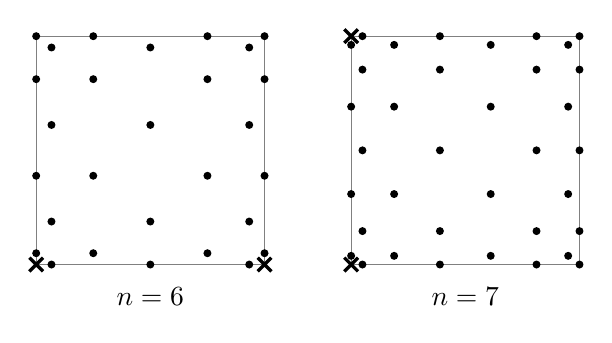
\begin{tikzpicture}[x=1.45cm,y=1.45cm]
\foreach \nn/\mm/\dx in {6/7/0,7/8/4} {
 \begin{scope}[xshift=\dx cm]
  \draw[gray] (-1,-1) rectangle (1,1);
  \foreach \jj in {0,...,\nn} {
   \foreach \kk in {0,...,\mm} {
    \pgfmathtruncatemacro{\parity}{mod(\jj+\kk,2)}
    \ifnum\parity=0
     \fill ({cos(180*\jj/\nn)},{cos(180*\kk/\mm)}) circle (0.035);
    \fi
   }
  }
  \draw[very thick] (-1.06,-1.06)--(-0.94,-0.94)
                    (-1.06,-0.94)--(-0.94,-1.06);
  \ifnum\nn=6
   \draw[very thick] (0.94,-1.06)--(1.06,-0.94)
                     (0.94,-0.94)--(1.06,-1.06);
  \else
   \draw[very thick] (-1.06,0.94)--(-0.94,1.06)
                     (-1.06,1.06)--(-0.94,0.94);
  \fi
  \node[below] at (0,-1.12) {$n=\nn$};
 \end{scope}
}
\end{tikzpicture}
\caption{The Padua points for two consecutive degrees. Dots are interpolation
points; crosses mark the two corners where the Lebesgue function attains
its maximum. The change of orientation depends only on parity.}
\label{fig:padua-nodes}
\end{figure}

Let $L_B$ be the cardinal polynomial associated with $B\in\mathcal P_n$.
Here \emph{cardinal polynomial} means the unique element of $\Pi_n$
whose value at $B$ is one and whose value at every other interpolation
node is zero. The collection of these polynomials is a basis adapted to
sampled values: a polynomial $p\in\Pi_n$ is reconstructed as
$p(z)=\sum_B p(B)L_B(z)$. In particular,
\[
 \sum_{B\in\mathcal P_n}L_B(z)=1,
\]
because the constant polynomial one is reproduced. Individual $L_B(z)$
can have either sign. The sum of their absolute values records how
large an arbitrary signed combination of the nodal data can become.
The Lebesgue function and its maximum are
\[
 \lambda_n(z)=\sum_{B\in\mathcal P_n}|L_B(z)|,
 \qquad \Lambda_n=\max_{z\in[-1,1]^2}\lambda_n(z).
\]
The function $\lambda_n$ is continuous, since it is a finite sum of
absolute values of polynomials. The square is compact, so the displayed
maximum exists. The identity $\sum_B L_B=1$ and the triangle inequality
give $\lambda_n(z)\geq1$ everywhere. At a node only one cardinal term
is nonzero, so there the lower bound is attained. This makes the values
between nodes especially relevant for stability.

For a real number $u$, the sign $\operatorname{sgn}u$ is $1$ when
$u>0$, $-1$ when $u<0$, and $0$ when $u=0$. At a fixed location
$z$, prescribe the data $e_B=\operatorname{sgn}L_B(z)$, choosing any
value of size at most one when a cardinal value is zero.
The corresponding interpolated value at $z$ is then exactly
$\sum_B|L_B(z)|$. Thus the absolute-value sum is the actual worst case
for bounded nodal data at that point. The sign choice can depend on $z$;
the Lebesgue function describes the worst case separately at each
location. Section~\ref{sec:preliminaries} also explains why these nodal
values may be extended to a continuous function of norm at most one,
which identifies $\Lambda_n$ with the operator norm on $C(Q)$.

At an interpolation point the Lebesgue function is exactly one. Away from
the points, its individual cardinal terms can reinforce each other.
For Padua interpolation the largest reinforcement occurs at the two corners
that are not interpolation points. This location was conjectured in
\cite{CaliariDeMarchiSommarivaVianello2008poster} and recorded among the
open problems in \cite[Section~3.3]{DeMarchi2022}.
Our first result identifies these maximizers exactly.

\begin{theorem}[Location of the maximum]\label{thm:main-location}
For every integer $n\geq2$, the maximum of $\lambda_n$ on the closed square
is attained exactly at
\[
 \begin{cases}
 \{(-1,-1),(1,-1)\},&n\text{ even},\\
 \{(-1,-1),(-1,1)\},&n\text{ odd}.
 \end{cases}
\]
In particular, $\Lambda_n=\Lambda_c(n)$, where
$\Lambda_c(n):=\lambda_n(-1,-1)$.
\end{theorem}

\noindent\textbf{The strength of the location assertion.}
An upper bound for $\Lambda_n$ would estimate the height of the graph
of $\lambda_n$. The theorem also determines all the locations reaching
that height. The word ``exactly'' includes the interior, all four edges,
the sampled points and every other corner: each point outside the
displayed pair has a strictly smaller value. This explains the need for
strict inequalities in the global argument. A dense plot can suggest
the two corners very convincingly, but the proof must control each
point of a continuum and must preserve equality information.

The equality between the values at the two listed corners comes from
a symmetry of the node set. For even $n$ the square can be reflected
in the vertical axis while preserving the nodes. For odd $n$ the
corresponding symmetry is reflection in the horizontal axis. Uniqueness
of interpolation transfers that geometric symmetry to $\lambda_n$.
The substantive global issue is the strict comparison with every other
point. Once it is resolved, a single scalar value
$\Lambda_c(n)=\lambda_n(-1,-1)$ determines the full norm.

The location proof is computer-assisted. Analytic estimates give the result
for $n\geq512$; rigorous finite certificates cover the remaining degrees.
The certificates bound the function on regions covering the square.
Sections~\ref{sec:argmax} and~\ref{sec:certificates} give these arguments
and their arithmetic assumptions.

Knowing the location reduces the Lebesgue constant to a single corner
value. Our second result describes that value much more precisely than
its leading growth rate. Here Euler's constant is
$\gamma=\lim_{R\to\infty}(H_R-\log R)$, where
$H_R=\sum_{r=1}^R r^{-1}$. Write
\begin{equation}\label{eq:main-constants}
 a=\frac2\pi,\qquad d=\gamma+\log\frac8\pi,\qquad
 c_1=ad,\qquad b=2ac_1,\qquad c=c_1^2+\kappa,
\end{equation}
with
\begin{equation}\label{eq:main-kappa}
 \kappa=\frac8\pi\int_0^1 t^2\cot\frac{\pi t}{2}
       \sum_{\substack{\ell\geq1\\\ell\text{ odd}}}
       \frac{1}{\ell(\ell^2-t^2)}\,dt.
\end{equation}
The apparent singularity at $t=1$ is canceled by the cotangent factor;
we justify convergence below.

\noindent\textbf{Reading the constants and the integral.}
The logarithms in this paper are natural logarithms. With $N=n+1/2$,
the letters in \eqref{eq:main-constants} package the coefficients of a square:
\[
 a^2\log^2N+b\log N+c
      =(a\log N+c_1)^2+\kappa
      =\frac4{\pi^2}(\log N+d)^2+\kappa.
\]
This identity is useful when tracing the two harmonic sums in the
corner calculation. Each has a logarithmic leading term and a constant
term. Multiplying them produces the squared logarithm, a single
logarithm and a constant. The coupled part of the calculation supplies
the additional constant $\kappa$.

The sum in \eqref{eq:main-kappa} runs over the positive odd integers
$1,3,5,\ldots$. The $\ell=1$ term deserves separate attention near
$t=1$. For every $0\leq t\leq1$ and integer $\ell\geq3$,
\[
 \ell^2-t^2\geq\ell^2-1\geq\frac89\ell^2,
 \qquad
 0\leq\frac1{\ell(\ell^2-t^2)}\leq\frac9{8\ell^3}.
\]
The last bound has a convergent sum: for example,
$\sum_{\ell=L}^{\infty}\ell^{-3}$ is at most
$L^{-3}+\int_L^{\infty}x^{-3}\,dx=L^{-3}+1/(2L^2)$.
It follows that the tail of the series over odd $\ell\geq3$ is
bounded by a quantity tending to zero independently of $t$. This is
uniform convergence on $[0,1]$. Each summand is continuous there, so
this part of the sum is a bounded continuous function, including both
endpoints. The remaining term, $\ell=1$, is handled separately.
Near $t=0$,
$\cot(\pi t/2)$ is of size $1/t$, so the factor $t^2$ makes the
complete integrand of size $t$. Near $t=1$ the potentially singular
term contains
\[
 \frac{t^2\cot(\pi t/2)}{1-t^2},
 \qquad
 \lim_{t\uparrow1}
 \frac{t^2\cot(\pi t/2)}{1-t^2}=\frac\pi4.
\]
Indeed, $\cot(\pi t/2)=\tan(\pi(1-t)/2)$ and
$1-t^2=(1-t)(1+t)$. These elementary endpoint checks already explain
why the integral specifies a finite real number. The later proof gives
the precise estimates needed for its use in the asymptotic expansion.

\begin{theorem}[Sharp corner expansion]\label{thm:main-expansion}
Let $N=n+\tfrac12$. For the points \eqref{eq:nodes}, as $n\to\infty$,
\begin{equation}\label{eq:main-expansion}
 \Lambda_c(n)=\frac4{\pi^2}\log^2N+b\log N+c-\frac1N
            +O\!\left(\frac{\log N}{N^2}\right).
\end{equation}
The constants and the remainder estimate are the same for both parities.
More precisely, a finite constant $C$, independent of $n$, bounds the
absolute remainder by $C\log N/N^2$ for every integer $n\geq2$.
Consequently \eqref{eq:main-expansion} also holds for $\Lambda_n$.
\end{theorem}

\noindent\textbf{What the error term says.}
If $\mathcal{R}_n$ denotes the difference between $\Lambda_c(n)$ and the four
explicit terms in \eqref{eq:main-expansion}, the statement is
\[
 |\mathcal{R}_n|\leq C\frac{\log(n+1/2)}{(n+1/2)^2}
 \quad(n\geq2)
\]
for one finite constant $C$ that works for every degree and both
parities. In particular $N \mathcal{R}_n\to0$. The remainder is smaller than $1/N$, so the coefficient of
the reciprocal term $-1/N$ is determined. A leading
$O(\log n)$ estimate leaves the constant and reciprocal terms
undetermined. The content of the sharp expansion lies in keeping
track of contributions small enough to affect those terms.

The change from $n$ to $N=n+1/2$ also matters at this accuracy. For
example, elementary Taylor expansion gives
\[
 \log(n+\tfrac12)=\log n+\frac1{2n}+O(n^{-2}),
 \qquad
 \log^2(n+\tfrac12)=\log^2n+\frac{\log n}{n}
                         +O\!\left(\frac{\log n}{n^2}\right).
\]
The correction $(\log n)/n$ is larger than the final remainder in the
theorem. A shift of scale therefore changes the lower-order bookkeeping.
The scale $N$ absorbs the logarithmic reciprocal term, leaving the pure
$-1/N$ correction. Both parities share one formula at each of the scales
$n$, $m=n+1$ and $N=n+1/2$.

An asymptotic expansion describes the behavior along arbitrarily large
degrees. The theorem additionally states a uniform bound for every
$n\geq2$. As usual, once the tail estimate is proved, finitely many
remaining degrees can be absorbed by increasing a finite constant.
That observation concerns the remainder bound for the corner value;
the separate global location theorem still has its own pointwise proof.

The corner expansion is proved analytically. Its transfer to $\Lambda_n$
as $n\to\infty$ uses only the analytic $n\geq512$ part of
Theorem~\ref{thm:main-location}. The finite certificates also identify the
maximum in the remaining degrees; the same remainder constant can therefore
be chosen for all $n\geq2$.

The leading growth
$\Lambda_n=(4/\pi^2)\log^2n+O(\log n)$ is due to
Kolomoitsev and Lomako~\cite[Theorem~2.1 and the following Padua consequence]{KolomoitsevLomako2021}.
Their proof uses pointwise rhombic Lebesgue-function asymptotics of
Kuznetsova~\cite[Theorem~1]{Kuznetsova1995}; Pimenova's earlier equal-parameter
result concerns the corresponding odd periodic grid
\cite[Theorem~1]{Pimenova1979}. These periodic results form the background
for the leading Padua asymptotics.

The lower-order sizes had also been anticipated numerically. De Marchi's
empirical model was $((2/\pi)\log(n+1)+1.1)^2$
\cite[Section~1.1, pp.~3--5]{DeMarchi2005NearOptimal}.
Here the explicit constants are
$b\approx1.225522125742$, $c\approx1.846160310424$, and
$\kappa\approx0.919710118388$. Theorem~\ref{thm:main-expansion}
identifies their exact expressions and resolves the lower terms through
an error smaller than $1/n$. Its square
comes from two harmonic sums; $\kappa$ measures their coupling, and the
half-integer scale exposes the reciprocal correction.

Both proofs begin with the same corrected interpolation kernel. At the
corner its signs give an exact positive sum. Away from the corner, reflection
writes the Lebesgue function as a periodic envelope minus the cancellation
lost in taking absolute values. A single comparison with a completed model
then controls that envelope and the competing reflection defects. Near an
actual maximizing corner, a positive interpolation argument proves strict
quadratic descent. The finite certificates use that same interpolation
principle. This organization separates the two ideas that matter: computing
the corner value and showing why no other point can exceed it.

Here the \emph{envelope} is an explicit upper-bound function obtained
by taking absolute values of reflected kernel terms before combining
them. It is periodic in angular coordinates. A \emph{reflection defect}
is the amount by which that upper bound exceeds the value after the
signed terms have been combined; it measures the cancellation lost in
the triangle inequality. The \emph{completed model} is an auxiliary
comparison expression, defined in the global argument, that allows us
to estimate the finite envelope by isolating its common large-degree
behavior and controlling the remaining error.

A \emph{positive interpolation argument} uses nonnegative interpolation
weights to carry bounds on finitely many values over an entire region,
with a proved remainder bound when the interpolation is approximate.
For example, a convex combination of four vertex values cannot exceed
their largest value. This positivity belongs to the interpolation
weights in the comparison argument; the Padua cardinal polynomials
introduced above can have either sign. Finally, \emph{quadratic descent}
means that sufficiently near a maximizing corner the loss from the
corner value is bounded below by a positive constant times squared
angular displacement. Such a bound is strictly positive at every
nearby point with nonzero displacement and vanishes at the corner.

The Padua construction and its generating-curve and ideal descriptions
are classical~\cite{BosCaliariDeMarchiVianelloXu2006,BosDeMarchiVianelloXu2007}.
Related numerical geometry of local maxima is studied in
\cite{BialasCiezDeMarchiSuder2026}. Rigorous norm approximation by polynomial
meshes, including Padua examples, was developed in~\cite{Mesh2024}; our
certificates add strict exclusion near the maximizing corners, identifying
the equality set.
For the distinct Morrow--Patterson family,
\cite{MorrowPatterson2026} proves an $O(n^2)$ upper bound.

We derive the corner expansion in Section~\ref{sec:corner}, then establish
one comparison theorem and apply it to the global location in
Section~\ref{sec:argmax}. Section~\ref{sec:certificates} completes the finite
range and states the arithmetic and evidence dependencies.


\noindent\textbf{A route through the proof.}
The normalization section begins with finite-dimensional linear algebra.
It proves that the node values uniquely determine a polynomial and
derives the cardinal polynomials from a weighted scalar product. This
step fixes the coefficient of one exceptional highest-frequency term;
all subsequent numerical constants refer to that normalization.
The angular variables then turn the polynomial kernel into finite cosine
sums. Geometric-series identities and elementary trigonometry are the
basic tools for making those sums explicit.

The corner section evaluates those sums where their signs can be
organized exactly. It isolates the harmonic growth, the coupled integral
and the endpoint corrections. Keeping endpoint terms matters because
their total contribution can be of order $1/n$, the scale resolved by
the second theorem. The global comparison section instead studies
points throughout the square. There absolute values hide some of the
signed cancellation, so the proof measures that cancellation explicitly
and compares it with the available envelope bound. The finite-row
estimates quantify the comparison uniformly across the required regions.

Finally, the certificate section explains how polynomial bounds on
closed regions yield global strict inequalities. Closed regions may
overlap along their boundaries; including those boundaries makes the
cover complete. Regions containing a maximizing corner require an
equality-aware argument, since the upper bound is attained there.
The proof has two obligations: evaluate the corner value and exclude
every competing point. The corner expansion and the global comparison
address these two obligations.

The explanations below develop each construction when it is first
needed. The numbered statements and formulas retain the same roles
throughout: they specify the quantitative results to be proved, while
the intervening derivations explain the linear algebra, trigonometric
identities and estimates on which those results depend.

\section{The interpolation operator and its normalization}\label{sec:preliminaries}
Put $Q=[-1,1]^2$ and let $\Pi_n$ be the real polynomials of total degree
at most $n$.

\noindent\textbf{Existence and uniqueness as a linear algebra question.}
A finite set of points is called \emph{unisolvent for $\Pi_n$} when
every assignment of one real value to each point is realized by exactly
one polynomial in $\Pi_n$. Equivalently, the evaluation map
\[
 \mathcal E:\Pi_n\longrightarrow\mathbb R^{\mathcal P_n},
 \qquad \mathcal E(p)=(p(B))_{B\in\mathcal P_n},
\]
is a bijection. The notation on the right means a real vector whose
coordinates are indexed by the nodes. Here the domain and target have
the same finite dimension. Consequently it suffices to prove that a
polynomial vanishing at every node must be the zero polynomial. Indeed,
that condition makes the linear map injective; a square injective
linear map is also surjective.

The standard unit vector associated with a node $B$ has entry one at
$B$ and entry zero at every other node. The cardinal polynomial $L_B$
is its inverse image under the evaluation map. Thus existence of all
the cardinal polynomials,
uniqueness of interpolation and invertibility of the evaluation matrix
are equivalent descriptions of the same fact. Lemma~\ref{lem:cardinal-kernel}
will establish that fact by computing a weighted sum of products of
basis values. The weights are positive, which will turn a vanishing
vector of values into a vanishing vector of coefficients.

The cardinal polynomials satisfy $L_B(A)=\delta_{AB}$ for
$A,B\in\mathcal P_n$, and
\[
 I_nf(z)=\sum_{B\in\mathcal P_n} f(B)L_B(z).
\]
The triangle inequality gives $\|I_n\|\leq\max_Q\lambda_n$; equality
follows by prescribing at the nodes the signs of the cardinal values
at a maximizing point and extending these finitely many values
continuously to $Q$. This proves the operator-norm interpretation used
in \eqref{eq:lebesgue-inequality}.

Here $\delta_{AB}$ is the Kronecker delta: it is one if $A=B$ and zero
otherwise. To give the norm argument in full, fix $z\in Q$. Then
\[
 |I_nf(z)|\leq\sum_B|f(B)|\,|L_B(z)|
       \leq\|f\|_\infty\lambda_n(z).
\]
Taking the maximum in $z$ gives the upper bound. For the reverse bound,
choose a point $z_*$ maximizing $\lambda_n$ and prescribe
$s_B=\operatorname{sgn}L_B(z_*)$. Recall that the sign of a positive
number is one, the sign of a negative number is minus one, and the sign
of zero is zero. The finite collection of distinct nodes has a positive minimum
separation. Choose $\rho>0$ so small that the closed balls of radius
$\rho$ around distinct nodes are disjoint, and put
\[
 \mathsf{h}_B(z)=\max\{0,1-|z-B|/\rho\},\qquad
 f_*(z)=\sum_B s_B\mathsf{h}_B(z),\qquad z\in Q.
\]
The norm $|z-B|$ here is Euclidean distance. Each $\mathsf{h}_B$ is continuous,
equals one at its own node and vanishes at the others. At any location
at most one summand is nonzero, so $|f_*(z)|\leq1$. Thus $f_*\in C(Q)$,
$f_*(B)=s_B$, and
\[
 I_nf_*(z_*)=\sum_B\operatorname{sgn}L_B(z_*)L_B(z_*)
              =\lambda_n(z_*).
\]
This constructs an admissible input attaining the bound. It also shows
why allowing continuous inputs supplies every bounded vector of nodal
values needed in the operator-norm argument.

\noindent\textbf{Why cosine polynomials are a convenient basis.}
The Chebyshev identity below specifies an ordinary algebraic polynomial
in $x=\cos t$. The first examples are
\[
 T_0(x)=1,\quad T_1(x)=x,\quad T_2(x)=2x^2-1,
 \quad T_3(x)=4x^3-3x.
\]
The cosine addition formula yields
$T_{r+1}(x)=2xT_r(x)-T_{r-1}(x)$, starting with $T_0,T_1$.
It follows inductively that $T_r$ has degree $r$ with nonzero leading
coefficient. Hence $T_0,\ldots,T_n$ form a basis for one-variable
polynomials of degree at most $n$. In two variables the products
$T_p(x)T_q(y)$ with $p+q\leq n$ form a basis for $\Pi_n$:
their leading monomials are nonzero multiples of $x^py^q$, and the
remaining terms have lower total degree. Successive elimination by
degree therefore changes between this basis and the monomial basis.
We call $(p,q)$ a \emph{mode index}; it records the two cosine
frequencies after the change to angular variables.

We use the Chebyshev polynomials $T_r(\cos t)=\cos(rt)$. Write
$\theta_j=j\pi/n$, $\phi_k=k\pi/(n+1)$ and
\[
 \varepsilon_j=\begin{cases}1/2,&j=0,n,\\1,&\text{otherwise},\end{cases}
 \qquad
 \eta_k=\begin{cases}1/2,&k=0,n+1,\\1,&\text{otherwise},\end{cases}
 \qquad w_{jk}=\frac{2\varepsilon_j\eta_k}{n(n+1)}.
\]
The endpoint factors are the half weights familiar from the trapezoidal
rule. Here they give an exact finite identity. A point interior to both angular grids has
weight $2/[n(n+1)]$; a point on one side has half that weight; a retained
corner has one quarter of that interior weight. All these numbers are
strictly positive.

The factor two compensates for retaining one color of the array. More
precisely, the \emph{checkerboard scalar product} is the weighted sum
\[
 \langle f,g\rangle_{\mathcal P_n}
   :=\sum_{\substack{0\leq j\leq n,\ 0\leq k\leq n+1\\j+k\ \mathrm{even}}}
        w_{jk}f(\cos\theta_j,\cos\phi_k)
               g(\cos\theta_j,\cos\phi_k).
\]
The expression is bilinear: holding one input fixed, it is linear in
the other input. For example,
\[
 \langle af_1+bf_2,g\rangle_{\mathcal P_n}
 =a\langle f_1,g\rangle_{\mathcal P_n}
   +b\langle f_2,g\rangle_{\mathcal P_n}
\]
for all real $a,b$. It is symmetric because exchanging $f$ and $g$
leaves every summand unchanged. It is initially positive semidefinite
on polynomials:
$\langle p,p\rangle_{\mathcal P_n}$ is a sum of nonnegative terms,
and it vanishes exactly when $p$ vanishes at every node. The lemma will
show that this form is positive definite on $\Pi_n$, meaning that it is
strictly positive for every nonzero element of that space. This is the
promised route to unisolvence. For arbitrary functions on the node set,
it is already the usual weighted Euclidean scalar product of their
vectors of values.

For the kernel formula below, set $\nu_0=1$ and $\nu_r=2$ for $r>0$;
these are the mode multiplicities. Write $z=(z_1,z_2)$ and
$B=(B_1,B_2)$ for physical points. In a sum with condition $p+q\leq n$,
both indices are nonnegative integers. If
$B=(\cos\theta_j,\cos\phi_k)$ is a node, the abbreviated notation
$w_B$ means $w_{jk}$. Define
\[
 K_n(z,B)=\sum_{p+q\leq n}\nu_p\nu_q
 T_p(z_1)T_p(B_1)T_q(z_2)T_q(B_2).
\]

The word \emph{kernel} here refers to a function of two points, formed
by summing products of matching basis functions. It is a finite
polynomial sum in $z$ and $B$. A \emph{reproducing kernel} for a scalar
product has the additional property that its scalar product with a
polynomial returns that polynomial's value at the other point. We
derive that property explicitly in the proof. The displayed $K_n$ has
the familiar coefficients $1$ for a zero frequency and $2$ for a
positive frequency in each coordinate. The grid gives one endpoint
mode a different squared norm, requiring the correction in the lemma.

One can anticipate the usual coefficients from the elementary integral
\[
 \frac1\pi\int_0^\pi\cos(pt)\cos(rt)\,dt
  =\begin{cases}1,&p=r=0,\\1/2,&p=r>0,\\0,&p\ne r.\end{cases}
\]
For a nonzero integer $k$, an antiderivative gives
\[
 \int_0^\pi\cos(kt)\,dt
   =\frac{\sin(k\pi)-\sin0}{k}=0.
\]
To obtain the displayed scalar products, use
\[
 \cos(pt)\cos(rt)
   =\tfrac12\cos((p-r)t)+\tfrac12\cos((p+r)t).
\]
When $p\ne r$, both cosine frequencies are nonzero and both integrals
vanish. When $p=r>0$, the first cosine is the constant one and the
second has nonzero frequency, giving $1/2$ after division by $\pi$.
When $p=r=0$, the integrand itself is one. The factors $\nu_r$ are
the reciprocals of these continuous squared norms. Sampling on an angular grid preserves this orthogonality for
the required indices but changes the highest available frequency in
the first coordinate. Since the two grids have sizes $n$ and $n+1$,
that change occurs asymmetrically. The proof computes it using finite
sums, so it also verifies exactly which continuous normalization survives
in the sampled setting.

The phrase \emph{cardinal kernel} in the lemma means that the corrected
kernel, with the weight of its second node attached, produces the
cardinal polynomial for that node. More explicitly, write temporarily
\[
 \widetilde K_n(z,B):=K_n(z,B)-T_n(z_1)T_n(B_1).
\]
The proof will show both that $\widetilde K_n$ reproduces $\Pi_n$ in the
checkerboard scalar product and that $w_B \widetilde K_n(A,B)=\delta_{AB}$ at
nodes. The weight belongs to the sampled variable $B$, just as a
quadrature weight belongs to the variable being summed. Later we
express this same $\widetilde K_n$ using angle sums and differences. The angular
kernel $G_n$ introduced after the proof is the two-angle trigonometric
sum from which those reflected copies of $\widetilde K_n$ are assembled. Thus
cardinal values, reproduction and the angular formula are linked by
explicit finite identities.

\begin{lemma}[Cardinal kernel]\label{lem:cardinal-kernel}
The set $\mathcal P_n$ is unisolvent for $\Pi_n$, and for
$B=(\cos\theta_j,\cos\phi_k)\in\mathcal P_n$,
\begin{equation}\label{eq:cardinal-kernel}
 L_B(z)=w_{jk}\bigl[K_n(z,B)-T_n(z_1)T_n(B_1)\bigr].
\end{equation}
In particular the coefficient of the highest first-coordinate mode is
one.
\end{lemma}
\begin{proof}
We first compute a one-dimensional weighted cosine sum. We then use
the parity condition to transfer that computation to the two-dimensional
node set. Finally we translate orthogonality into the inverse of the
interpolation system. All sums in this proof are finite.

\noindent\textbf{The endpoint-weighted geometric sum.}
For $M\geq1$ let
\[
 Q_M(g)=\frac1M\sum_{j=0}^M{}'g(j\pi/M),
\]
where the prime gives weight $1/2$ to each endpoint. The symbol $g$
denotes a function of the angle $t$. Thus $Q_M(\cos rt)$ means that
$g(t)=\cos(rt)$. The total of the weights before division by $M$ is
$M$, so $Q_M(1)=1$.

Recall the finite geometric-series identity
\[
 \sum_{j=0}^M z^j=\frac{1-z^{M+1}}{1-z}\quad(z\ne1).
\]
It follows by multiplying the sum by $1-z$: all middle powers cancel.
We use elementary complex-number notation to evaluate this sum.
A complex number is written $a+ib$, where $a,b$ are real and $i^2=-1$;
its real part is $\operatorname{Re}(a+ib)=a$. We use
$e^{i\alpha}=\cos\alpha+i\sin\alpha$ for real $\alpha$. The angle
addition formulas give $e^{i\alpha}e^{i\beta}=e^{i(\alpha+\beta)}$,
so $(e^{i\alpha})^j=e^{ij\alpha}$ and its real part is
$\cos(j\alpha)$. Only these finite algebraic identities are required
here.

To evaluate the cosine sum, let $r$ be an integer with
$1\leq r\leq2M-1$, set $z=e^{ir\pi/M}$, and write
$\sigma=z^M=(-1)^r$. In this range $z\ne1$. Half weighting the two
endpoints subtracts $(1+z^M)/2$ from the full geometric sum. Thus
\[
 \sum_{j=0}^M{}'z^j
 =\frac{1-\sigma z}{1-z}-\frac{1+\sigma}2
 =\frac{(1-\sigma)(1+z)}{2(1-z)}.
\]
For even $r$, $\sigma=1$ and this expression is zero. For odd $r$,
the quotient $(1+z)/(1-z)$ is purely imaginary. Writing
$z=e^{i\alpha}$ gives
\[
 \frac{1+e^{i\alpha}}{1-e^{i\alpha}}
   =i\cot\frac\alpha2.
\]
Indeed, factoring $e^{i\alpha/2}$ out of numerator and denominator
gives
\[
 \frac{2e^{i\alpha/2}\cos(\alpha/2)}
      {-2ie^{i\alpha/2}\sin(\alpha/2)}
 =i\frac{\cos(\alpha/2)}{\sin(\alpha/2)}.
\]
Here $1/i=-i$ follows from $i^2=-1$, and the denominator is nonzero
because $e^{i\alpha}\ne1$. The cotangent is real for these real
angles, so the expression has real part zero. Taking real parts in
the weighted geometric sum gives zero in both parity cases. Since
$\operatorname{Re}z^j=\cos(rj\pi/M)$, the weighted cosine average
vanishes. For $r=2M$ every cosine value is one, so its average is one.
This explains why the upper frequency $2M$ has to be kept separate
from the preceding vanishing range. We have proved
$Q_M(\cos rt)=0$ for $1\leq r\leq2M-1$ and
$Q_M(1)=Q_M(\cos2Mt)=1$.

Using $\cos(-t)=\cos t$, the same values apply to negative integer
frequencies. For $0\leq p,r\leq M$ the product identity
\[
 \cos(pt)\cos(rt)=\tfrac12\cos((p-r)t)
                         +\tfrac12\cos((p+r)t)
\]
now computes the scalar products. If $p\ne r$, both frequencies have
absolute value between $1$ and $2M-1$, so both averages vanish. If
$p=r$ with $0<p<M$, the constant frequency contributes $1/2$ and
the frequency $2p$ contributes zero. At $p=r=0$ both contributions
are constant, and at $p=r=M$ the frequencies are $0$ and $2M$;
the answer is one in both endpoint cases. Consequently
\[
 Q_M(\cos pt\cos rt)=\delta_{pr}h_p^{(M)},\qquad
 h_p^{(M)}=\begin{cases}1,&p=0,M,\\1/2,&0<p<M.\end{cases}
\]
Thus $h_p^{(M)}$ is the squared length of the $p$th cosine mode in this
discrete scalar product. At the highest mode, the sampled values are
$\cos(Mj\pi/M)=(-1)^j$, whose square is one at every grid point.
This gives a direct explanation of $h_M^{(M)}=1$.

\noindent\textbf{What selecting the checkerboard does.}
Put $e_{pq}(x,y)=T_p(x)T_q(y)$, where $p+q\leq n$.
The \emph{Gram matrix} is the matrix whose entry indexed by $(p,q)$
and $(r,s)$ is $\langle e_{pq},e_{rs}\rangle_{\mathcal P_n}$.
A Gram matrix records all pairwise scalar products of a chosen basis.
Its diagonal entries are the squared lengths of the basis vectors, and
an off-diagonal zero expresses orthogonality. We compute each entry
with the parity restriction included.

The indicator of an even index sum satisfies
\[
 2\mathbf1_{j+k\,\mathrm{even}}=1+(-1)^j(-1)^k.
\]
An indicator is one when its subscripted condition holds and zero
otherwise. Inserting this identity into the weighted sum extends it to
the full rectangular array and splits it into two products of
one-dimensional sums. Explicitly, the entry is
\begin{align*}
 &Q_n(\cos(pt)\cos(rt))\,
       Q_{n+1}(\cos(qt)\cos(st))\\
 &\quad+
 \left(\frac1n\sum_{j=0}^n{}'(-1)^j
                    \cos(p\theta_j)\cos(r\theta_j)\right)
 \left(\frac1{n+1}\sum_{k=0}^{n+1}{}'(-1)^k
                    \cos(q\phi_k)\cos(s\phi_k)\right).
\end{align*}
The first line is the tensor product part: ``tensor product'' here
means the product of an independent sum in each coordinate. The
second line is the alternating part caused by the choice of color.

At the grid angles $t_j=j\pi/M$, the identity
\[
 \cos((M-p)t_j)
 =\cos(Mt_j)\cos(pt_j)+\sin(Mt_j)\sin(pt_j)
 =(-1)^j\cos(pt_j)
\]
holds because $\sin(j\pi)=0$. Thus multiplication by $(-1)^j$
sends mode $p$ to mode $M-p$ on the grid. The first alternating factor
is $Q_n(\cos((n-p)t)\cos(rt))$, which can be nonzero only if
$r=n-p$. The second factor can be nonzero only if $s=n+1-q$.
All these indices lie in the one-dimensional orthogonality ranges
already proved. In particular $q,s\leq n<n+1$.

For the product to survive, both necessary equalities must hold at once.
They would imply
\[
 p+r=n,\qquad q+s=n+1,\qquad p+r+q+s=2n+1.
\]
But the two mode indices are admissible, so
$(p+q)+(r+s)\leq2n$. This contradiction makes the alternating part
zero. It is exactly here that the triangular mode constraint and the
two consecutive grid sizes work together. The tensor product part is
computed by the one-dimensional identity. Therefore
\[
 \langle e_{pq},e_{rs}\rangle_{\mathcal P_n}
 =\delta_{pr}\delta_{qs}h_p^{(n)}h_q^{(n+1)}.
\]
The Gram matrix is diagonal and positive, with diagonal
$h_p^{(n)}h_q^{(n+1)}$. In particular the $(0,0)$ entry equals one,
so the nodal weights sum to one.

\noindent\textbf{Positive Gram matrix and interpolation.}
Expand a polynomial as $P=\sum_{p+q\leq n}c_{pq}e_{pq}$.
The orthogonality identity gives
\[
 \langle P,P\rangle_{\mathcal P_n}
  =\sum_{p+q\leq n}c_{pq}^2h_p^{(n)}h_q^{(n+1)}.
\]
Each factor on the right is positive. If $P$ vanishes at every node,
the left side is zero. Each coefficient must therefore vanish, proving
injectivity of the evaluation map. There are $(n+1)(n+2)/2$
checkerboard points, the same number as the modes, so the evaluation
map is also surjective. This proves unisolvence.

In matrix notation, choose any fixed ordering of the nodes and mode
indices, and let
\[
 E_{B,(p,q)}=e_{pq}(B),\qquad
 W=\operatorname{diag}(w_B),\qquad
 D=\operatorname{diag}(h_p^{(n)}h_q^{(n+1)}).
\]
Here $\operatorname{diag}$ denotes the matrix with the listed entries
on its diagonal and zeros elsewhere; $w_B$ is $w_{jk}$ at node $B$.
The transpose $E^{\mathsf T}$ exchanges row and column indices.
Matrix multiplication sums products over the shared index. Since $W$
is diagonal, the entry of the product indexed by the two modes is
\begin{align*}
 (E^{\mathsf T}WE)_{(p,q),(r,s)}
 &=\sum_{B\in\mathcal P_n}
       E_{B,(p,q)}w_BE_{B,(r,s)}\\
 &=\sum_{B\in\mathcal P_n}w_B e_{pq}(B)e_{rs}(B)
   =\langle e_{pq},e_{rs}\rangle_{\mathcal P_n}.
\end{align*}
Our orthogonality calculation makes this entry zero for distinct modes
and $h_p^{(n)}h_q^{(n+1)}$ for identical modes. These are exactly the
entries of $D$, proving $E^{\mathsf T}WE=D$. To see explicitly why
this implies independent columns, suppose a coefficient vector $c$
satisfies $Ec=0$. Then
\[
 c^{\mathsf T}Dc=(Ec)^{\mathsf T}W(Ec)=0.
\]
The left side is a sum of strictly positive diagonal factors times the
squares of the entries of $c$. Consequently all those entries vanish,
which is precisely column independence. Since $E$ is square, it is invertible. This matrix
expression also tracks the kernel normalization.

For $q\leq n$, the inverse of $h_q^{(n+1)}$ is $\nu_q$. In the
first coordinate the inverse of $h_p^{(n)}$ is $\nu_p$ for $p<n$,
while the inverse at $p=n$ is one. The only admissible mode with $p=n$
has $q=0$. Thus the inverse Gram coefficients are $\nu_p\nu_q$ except
at $(p,q)=(n,0)$, where the coefficient is one. Precisely one product
coefficient differs from the continuous normalization described above.

\noindent\textbf{Why a reproducing kernel yields the cardinal values.}
Define the kernel with these inverse coefficients by
\[
 \widetilde K_n(z,B)=\sum_{p+q\leq n}
   \frac{e_{pq}(z)e_{pq}(B)}{h_p^{(n)}h_q^{(n+1)}}
        =K_n(z,B)-T_n(z_1)T_n(B_1).
\]
For a fixed $z$, take its scalar product in the $B$ variable with
$P(B)=\sum_{r+s\leq n}c_{rs}e_{rs}(B)$. Substituting both finite
expansions and interchanging finite sums gives
\begin{align*}
 &\sum_{B\in\mathcal P_n}w_B \widetilde K_n(z,B)P(B)\\
 &\quad=\sum_{p+q\leq n}\sum_{r+s\leq n}
    \frac{e_{pq}(z)c_{rs}}{h_p^{(n)}h_q^{(n+1)}}
       \sum_{B\in\mathcal P_n}w_Be_{pq}(B)e_{rs}(B)\\
 &\quad=\sum_{p+q\leq n}\sum_{r+s\leq n}
    \frac{e_{pq}(z)c_{rs}}{h_p^{(n)}h_q^{(n+1)}}
          \langle e_{pq},e_{rs}\rangle_{\mathcal P_n}.
\end{align*}
The inner scalar product is zero unless $r=p$ and $s=q$. For those
surviving indices its value is $h_p^{(n)}h_q^{(n+1)}$, exactly
canceling the denominator. Hence the double sum reduces to the single
basis expansion and yields
\[
 \sum_{B\in\mathcal P_n}w_B \widetilde K_n(z,B)P(B)
      =\sum_{p+q\leq n}c_{pq}e_{pq}(z)=P(z).
\]
This is the reproducing property: the weighted scalar product with
$\widetilde K_n(z,\cdot)$ returns evaluation at $z$ for every $P\in\Pi_n$.

To see the nodal delta values directly, let $F$ be the matrix with
entries $F_{A,B}=w_B \widetilde K_n(A,B)$. To obtain its matrix formula, compute
one entry of the proposed product:
\begin{align*}
 (ED^{-1}E^{\mathsf T}W)_{A,B}
 &=w_B\sum_{p+q\leq n}
       \frac{e_{pq}(A)e_{pq}(B)}{h_p^{(n)}h_q^{(n+1)}}\\
 &=w_B\widetilde K_n(A,B)=F_{A,B}.
\end{align*}
The equality of all entries proves the formula for $F$. Associating
matrix factors and then using $E^{\mathsf T}WE=D$ gives
\[
 F=ED^{-1}E^{\mathsf T}W,
 \qquad FE=ED^{-1}(E^{\mathsf T}WE)=E.
\]
Multiplying $FE=E$ on the right by $E^{-1}$ gives $F$ equal to the
identity matrix. Hence $w_B \widetilde K_n(A,B)=\delta_{AB}$. For fixed $B$,
the function $w_B \widetilde K_n(z,B)$ lies in $\Pi_n$ and has precisely the
prescribed cardinal values. Uniqueness identifies it with $L_B$ and
proves \eqref{eq:cardinal-kernel}. The exceptional coefficient in $K_n$
was $\nu_n\nu_0=2$; subtracting one copy of its product leaves
coefficient one, as claimed.
\end{proof}

\noindent\textbf{A complete small example of the normalization.}
The case $n=1$ provides a short illustration of the kernel construction.
Although the main location theorem is stated from degree two onward,
the interpolation identities in this section already apply at degree
one. The nodes are
\[
 B_1=(1,1),\qquad B_2=(1,-1),\qquad B_3=(-1,0),
\]
with respective weights $1/4,1/4,1/2$. In the basis $1,x,y$, the
weighted Gram matrix is diagonal with entries $1,1,1/2$. For instance,
\[
 \langle1,x\rangle_{\mathcal P_1}
       =\tfrac14+\tfrac14-\tfrac12=0,
 \qquad
 \langle x,x\rangle_{\mathcal P_1}=1,
 \qquad
 \langle y,y\rangle_{\mathcal P_1}=\tfrac12.
\]
The distinction between the last two squared norms reflects the two
unequal grids.

For $z=(x,y)$ and $B=(\xi,\eta)$, the uncorrected sum and the
corrected sum are
\[
 K_1(z,B)=1+2x\xi+2y\eta,\qquad
 R_1(z,B)=1+x\xi+2y\eta.
\]
Multiplying the corrected expression by each nodal weight gives
\[
 L_{B_1}(x,y)=\frac{1+x+2y}{4},\qquad
 L_{B_2}(x,y)=\frac{1+x-2y}{4},\qquad
 L_{B_3}(x,y)=\frac{1-x}{2}.
\]
Substituting the three node coordinates verifies all nine cardinal
values directly. Summing the formulas gives one. The exceptional
$x\xi$ coefficient is visibly one: replacing it by two would alter
the nodal values and the interpolating polynomial. This example shows
how a single normalization coefficient affects the entire construction.

It also illustrates the absolute values in the Lebesgue function.
For real $a,b$,
\[
 |a+b|+|a-b|=2\max(|a|,|b|).
\]
To prove this, first suppose $|a|\geq|b|$. If $a\geq0$, then both
$a+b$ and $a-b$ are nonnegative and their absolute values sum to
$2a=2|a|$. If $a<0$, both are nonpositive and the sum is $-2a=2|a|$.
In the other case, $|b|\geq|a|$, exchange $a$ and $b$ in that
argument; the left side is unchanged because $|b-a|=|a-b|$, and the
answer is $2|b|$. This includes equality and zero cases.

For the first two cardinal polynomials, apply the identity with
$a=1+x$ and $b=2y$ and divide by four. On $Q$, $1+x$ and $1-x$ are
nonnegative, so the third cardinal polynomial already has nonnegative
value. Therefore
\[
 \lambda_1(x,y)
 =\max\left(\frac{1+x}{2},|y|\right)+\frac{1-x}{2}
 =\max\left(1,|y|+\frac{1-x}{2}\right).
\]
For every $(x,y)\in Q$, both $|y|\leq1$ and $(1-x)/2\leq1$,
so the second entry in this maximum is at most two. It equals two
precisely when both bounds are equalities: $|y|=1$ and $x=-1$.
The first entry is one and cannot reach two. Thus the largest value
is two, attained exactly at $(-1,1)$ and $(-1,-1)$.
All of this follows from the displayed affine polynomials. For larger
$n$ there are many more changing signs; the kernel representation
organizes those signs in a way suited to the later proofs.

\noindent\textbf{Passing from physical coordinates to angles.}
Every $z=(x,y)\in Q$ can be written uniquely as
$z=(\cos\theta,\cos\phi)$ with $\theta,\phi\in[0,\pi]$.
In these variables every $T_p(x)T_q(y)$ becomes
$\cos(p\theta)\cos(q\phi)$. A polynomial kernel of two physical
points therefore becomes a trigonometric expression involving four
angles. The \emph{angular kernel} is the finite sum in two free angle
variables $u,v$ that lets us express the four-angle kernel as an average
of reflected copies. Its definition below includes the same exceptional
mode correction already determined by the scalar product.

The same correction appears in the angular kernel
\begin{equation}\label{eq:angular-kernel}
 G_n(u,v)=\sum_{p+q\leq n}\nu_p\nu_q\cos(pu)\cos(qv)-\cos(nu).
\end{equation}
At a corner it gives the exact signed row sums; in the interior its
reflections give the cancellation comparison. Thus the two arguments
start from one normalized kernel.

To spell out the relation, write $B=(\cos\alpha,\cos\beta)$ and
$z=(\cos\theta,\cos\phi)$. The product-to-sum identity gives
\[
 \cos(p\theta)\cos(p\alpha)
    =\tfrac12\{\cos(p(\theta-\alpha))+
                         \cos(p(\theta+\alpha))\}.
\]
Applying it in both coordinates, including the corrected term, yields
\[
 \widetilde K_n(z,B)=\frac14\sum_{\sigma\in\{-1,1\}}
                    \sum_{\tau\in\{-1,1\}}
         G_n(\theta+\sigma\alpha,\phi+\tau\beta).
\]
The correction $-\cos(nu)$ in $G_n$ contributes
$-\cos(n\theta)\cos(n\alpha)$ to this average, because the sum in
$\tau$ simply supplies two equal copies. Thus it reproduces exactly
the correction in $\widetilde K_n$. Substituting node angles $\alpha=\theta_j$
and $\beta=\phi_k$ and multiplying by $w_{jk}$ recovers $L_B(z)$.

The function $G_n$ is a trigonometric polynomial: a finite linear
combination of products of sine or cosine functions, here consisting
only of cosine products. It is even in each angle and $2\pi$-periodic
in each angle. These properties justify reducing angle expressions
modulo $2\pi$ and reflecting them when convenient. Such reductions
apply to the angle arguments of $G_n$; the two different grid mesh
widths remain fixed throughout.

This representation explains why both angle sums and angle differences
appear in later formulas. They arise from multiplying a mode evaluated
at $z$ by the same mode evaluated at $B$. At a corner, $\theta$ and
$\phi$ are each either zero or $\pi$, so cosine values simplify to
signs and the two reflected contributions in a coordinate are closely
related. At an interior point their relative signs carry additional
information. For real numbers $a_1,\ldots,a_m$ the nonnegative quantity
\[
 \sum_{r=1}^m|a_r|-\left|\sum_{r=1}^m a_r\right|
\]
measures the cancellation lost if the absolute value is moved inside
the sum. Applying the triangle inequality to the four reflected copies
of $G_n$ produces precisely this kind of loss. Later comparisons retain
and estimate that loss, because its size helps distinguish a corner
from a competing point.

\noindent\textbf{Why the surviving reflections preserve interpolation.}



The two nonnode corners in Theorem~\ref{thm:main-location} have equal
Lebesgue values by symmetry. For even $n$, reflection in the first
coordinate sends $j$ to $n-j$ and preserves the checkerboard. For odd
$n$, reflection in the second coordinate sends $k$ to $n+1-k$ and
preserves it. Uniqueness of interpolation carries these symmetries to
the cardinal polynomials and hence to $\lambda_n$.

Here is the uniqueness argument explicitly. Let $S$ denote the relevant
coordinate reflection, so $S$ permutes $\mathcal P_n$ and $S^2$ is the
identity map. Composition with $S$ preserves total degree. At any node
$A$,
\[
 L_{SB}(SA)=\delta_{SA,SB}=\delta_{A,B}.
\]
Thus the polynomial $z\mapsto L_{SB}(Sz)$ has the same cardinal data
as $L_B(z)$ and belongs to the same space. Unisolvence gives
$L_{SB}(Sz)=L_B(z)$ for every $z\in Q$. Reindexing the sum of absolute
values by the node permutation $B\mapsto SB$ proves
\[
 \lambda_n(Sz)=\sum_{B\in\mathcal P_n}|L_{SB}(Sz)|
              =\sum_{B\in\mathcal P_n}|L_B(z)|=\lambda_n(z).
\]
For even $n$, the map $(j,k)\mapsto(n-j,k)$ changes $j+k$ by an even
integer and corresponds to $(x,y)\mapsto(-x,y)$. For odd $n$, the map
$(j,k)\mapsto(j,n+1-k)$ has the same parity property and corresponds
to $(x,y)\mapsto(x,-y)$. These maps exchange the two nonnode corners
listed in Theorem~\ref{thm:main-location}. This proves their equality
of value before the later strict global comparison is undertaken.

\noindent\textbf{Continuous values at quotient formulas.}
Finite cosine sums are continuous at every real angle. When a geometric
sum is written as a trigonometric quotient, its denominator can vanish
at some angles even though the original finite sum is perfectly
well-defined. A simple example is
\[
 \sum_{r=0}^{M-1}e^{irt}
    =e^{i(M-1)t/2}\frac{\sin(Mt/2)}{\sin(t/2)}
      \quad(t\notin2\pi\mathbb Z).
\]
At $t=0$ the left side equals $M$, and the quotient on the right has
that same limit. The polynomial or finite trigonometric expression
specifies the value at the exceptional angle. This convention applies
in particular when an evaluation angle meets a node angle, or when a
sum or difference of angles reaches an endpoint. Such events are called
\emph{collisions} below. They are included in every closed domain on
which a bound is asserted.


\begin{remark}
All formulas involving trigonometric quotients are interpreted by their
continuous polynomial limits at removable singularities. The maximization
and certificate domains include all nodes, edges and collisions of angular
coordinates.
\end{remark}

\section{The corner value: from exact rows to the first correction}
\label{sec:corner}

This section calculates the corner value of the Lebesgue function. Recall that the Lebesgue
function at a point is the sum of the absolute values of all cardinal
polynomials at that point. Its corner value is denoted by
$\Lambda_c(n)$. The calculation has three stages. First we turn the
finite sum into an exact sum of one-dimensional rows. Next we compare
with an equal-mesh problem to identify the limiting constant. Finally
we estimate the exact rows finely enough to find the term of size
$1/n$. Each stage uses a different feature of the same finite sum.

Two elementary ideas organize the calculation. A singular expression
can be easier to sum after its poles, meaning reciprocal singular
terms such as $c/(x-x_0)$, have been written explicitly;
what remains then has bounded derivatives. Also, a displacement of
size $1/n$ in a mesh can produce a constant change in a sum when the
summands are large near a diagonal. We shall see both effects. The
singularities in intermediate trigonometric quotients require care,
but the underlying cardinal polynomials are finite everywhere.

A Cauchy sum here means a sum containing reciprocal distances
$|x-y|^{-1}$. At a corner the absolute cardinal kernel becomes a positive Cauchy sum.
Its two meshes have sizes $n$ and $n+1$. The equal-mesh reference gives
the leading square; the mesh displacement supplies the constant defect
and the first correction. We retain that displacement throughout the proof.
Put $m=n+1$ and, for the rest of this section, write
\[
 \theta_j=j\pi/n,\quad \phi_k=k\pi/m,\qquad
 \varepsilon_j=\begin{cases}1/2,&j=0,n,\\1,&0<j<n,\end{cases}
 \quad \eta_k=\begin{cases}1/2,&k=0,m,\\1,&0<k<m.\end{cases}
\]
Every unspecified constant below is independent of $n\geq2$ and of the
row indices in their stated ranges. Set $A(z)=a(\log z+d)$, with the
constants in \eqref{eq:main-constants}.

Here and below $\log$ is the natural logarithm, $a=2/\pi$ and
$d=\gamma+\log(8/\pi)$. Thus $A(z)^2$ is an explicitly known
quadratic polynomial in $\log z$. The notation $O(E_n)$ means that
the absolute value of the omitted quantity is at most $CE_n$ for
some fixed finite constant $C$. A statement uniform in a row index
means that the same $C$ works for every row in the stated range.
This distinction will matter: an estimate proved with $r$ fixed as
$n$ grows does not automatically control the sum over $1\leq r\leq n$.

The weights $\varepsilon_j$ and $\eta_k$ are endpoint weights.
They implement the trapezoidal convention on the two angular grids:
an interior sample has weight one, and an endpoint sample has weight
one half. Their occurrence is also a consequence of reflection.
An interior angle has two representatives on a full period, whereas
an endpoint is fixed by reflection. The meshes differ by one in their
denominators throughout this section; in particular $\phi_n<\pi$,
while $\phi_m=\pi$.

\subsection{An exact row formula}

The first task is to understand the absolute values in the corner
sum. In its Cauchy denominators the coordinates are
$x_j=\cos\theta_j$ and $y_k=\cos\phi_k$.
These denominators become small when the angles
are close. The useful fact is that their signs, before taking absolute
values, change at a single position in each row. That allows an
absolute row to be reconstructed from its signed sum and its positive
part.

We begin with the exact kernel so that the endpoint contribution is
kept visible. The function $f$ below is used only when its two cosine
arguments are distinct. At an actual collision the original
trigonometric polynomial supplies the value; a quotient formula alone
cannot decide that value.
For $u\ne v$ let $f(u,v)=(1+\cos v)/|\cos u-\cos v|$. We first obtain
\begin{equation}\label{cu:positive}
 \Lambda_c(n)=\frac4{nm}
 \sum_{\substack{0\leq j,k\leq n\\j+k\text{ odd}}}
       \varepsilon_j\eta_k f(\theta_j,\phi_k)+\frac1m.
\end{equation}
To see this directly from \eqref{eq:cardinal-kernel}, define
$D_n(u,v)=\sum_{|p|+|q|\leq n}e^{i(pu+qv)}$. Grouping signs identifies
this with the product Chebyshev sum at a corner.

For clarity, the Chebyshev identity being used is
$T_p(\cos u)=\cos(pu)$. Combining the positive and negative
frequencies gives
\[
 \sum_{p=-P}^{P}e^{ipu}=1+2\sum_{p=1}^{P}\cos(pu).
\]
Applying this grouping in both coordinates shows that the diamond
sum $D_n$ has precisely the multiplicities $\nu_p\nu_q$ in the
kernel $K_n$, with total degree condition $p+q\leq n$.
At $(1,1)$ all the factors $T_p(1)$ equal one. At another corner,
$T_p(-1)=(-1)^p$ changes phases or reflects the node indices.
The separate correction $T_n(z_1)T_n(B_1)$ in the cardinal formula
remains essential after this grouping: it is the term that later
appears as $(-1)^j$. With
$S=(u+v)/2$, $T=(v-u)/2$, finite geometric sums give
\[
 D_n(u,v)=\frac{\sin((n+1)S)\sin((n+1)T)+\sin(nS)\sin(nT)}
                  {\sin S\sin T}.
\]
Indeed $(p,q)\mapsto(p+q,q-p)$ takes the diamond into the square
$[-n,n]^2$ with equal coordinate parity; summing its two parity classes
gives the displayed product.

The change of variables can be checked directly. If
$A=p+q$ and $B=q-p$, then
$p=(A-B)/2$, $q=(A+B)/2$, and
\[
 |p|+|q|=\max(|A|,|B|),\qquad pu+qv=AS+BT.
\]
The inverse indices are integers exactly when $A$ and $B$ have the
same parity. Thus the diamond is the union of an even-even and an
odd-odd rectangular grid in $(A,B)$. For a step-two progression,
\[
 \sum_{h=0}^{M}e^{i(-M+2h)z}
       =\frac{\sin((M+1)z)}{\sin z}.
\]
The two parity classes have progression lengths $n+1$ and $n$.
Multiplying their one-dimensional sums gives the two products of
sines in the formula for $D_n$. This derivation also explains why
the apparent singularities are removable: each sine quotient was
obtained from a finite sum of exponentials. Quotients at zero denominators have their
continuous polynomial values. Reflection of node indices about either
nonnode corner turns the checkerboard odd and leaves its weights unchanged.
The corresponding Lebesgue sum is therefore
$\sum_{j+k\text{ odd}}2\varepsilon_j\eta_k
 |D_n(\theta_j,\phi_k)-(-1)^j|/(nm)$.
Here the mesh identities are
$n\theta_j=j\pi$ and $m\phi_k=k\pi$. For example,
$\sin(m\theta_j)=(-1)^j\sin\theta_j$ and
$\sin(n\phi_k)=(-1)^{k+1}\sin\phi_k$.
Together with $j+k$ odd, these identities reduce the numerator of
$D_n$ to the expression below. The conversion from products of sines
to cosine differences uses
\[
 \cos u-\cos v
       =2\sin\frac{u+v}{2}\sin\frac{v-u}{2}.
\]
Once the correction is subtracted, the numerator simplifies further:
\[
 \frac{2+\cos u+\cos v}{\cos u-\cos v}-1
       =\frac{2(1+\cos v)}{\cos u-\cos v}.
\]
Since $1+\cos v\geq0$ on $[0,\pi]$, taking absolute values now
produces exactly the positive summand $2f(u,v)$.
\[
 D_n(\theta_j,\phi_k)=(-1)^j
       \frac{2+\cos\theta_j+\cos\phi_k}{\cos\theta_j-\cos\phi_k},
 \qquad |D_n(\theta_j,\phi_k)-(-1)^j|=2f(\theta_j,\phi_k).
\]
Coprimality of $n,m$ leaves only the collisions $(0,0)$ and $(n,m)$.
The odd checkerboard excludes the first. At the second,
$D_n(\pi,\pi)=(-1)^n(2n+1)$, so the corrected absolute value $2n$
with weight $1/(2nm)$ contributes $1/m$. The other entries with $k=m$
vanish. This proves \eqref{cu:positive} and the equality of the two
nonnode corner values. The node corners have value one by cardinality.

There are two small points in this reduction worth checking. First,
$\cos u=\cos v$ with $u,v\in[0,\pi]$ implies $u=v$,
because cosine is strictly decreasing there. Hence a collision of
the two meshes requires $jm=kn$. Since consecutive integers are
coprime, $j=0,k=0$ or $j=n,k=m$ are the only possibilities.
Second, the corner $k=m$ is absent from the double sum in
\eqref{cu:positive}. For $j<n$ its numerator is zero and its
contribution vanishes. At $j=n$ the quotient would be $0/0$,
so we evaluate the polynomial instead. Its endpoint weights give
$2\varepsilon_n\eta_m/(nm)=1/(2nm)$; multiplying by the
corrected absolute value $2n$ gives the displayed $1/m$.

A removable singularity is a point at which a formula is undefined
although the function it represents has a finite continuous extension.
The sine-quotient representation of the finite polynomial $D_n$
has this property. The function $f$ is used only at distinct sampled
angles; it has no joint continuous extension at $(\pi,\pi)$.
Neighboring unequal-mesh entries can be large. We keep their Cauchy denominators
because their size creates the logarithmic growth and the limiting
mesh defect.

The sign change within each row makes \eqref{cu:positive} effectively
one dimensional. We call a function analytic at a point when it is
represented there by a convergent power series on a neighborhood.
For an endpoint this neighborhood extends across the endpoint. Introduce
\begin{equation}\label{cu:wB}
 w(x)=\cot(\pi x/2),\qquad
 B(x)=\cot(\pi x)-\frac1{\pi x}+\frac1{\pi(1-x)}.
\end{equation}
Both poles have been removed from $B$; it is analytic across $[0,1]$,
with $B(0)=1/\pi$, $B(1)=-1/\pi$.

The subtraction in $B$ removes a pole at each end. Indeed, as
$x\to0$,
\[
 \cot(\pi x)=\frac1{\pi x}-\frac{\pi x}{3}+O(x^3),
 \qquad \frac1{\pi(1-x)}=\frac1\pi+O(x).
\]
This gives $B(0)=1/\pi$. At the other end put $y=1-x$ and use
$\cot(\pi(1-y))=-\cot(\pi y)$ to obtain $B(1)=-1/\pi$.
The same convergent power series give the asserted analytic
extensions. In particular
$B$ and all derivatives needed below are bounded on the closed
interval. The function $w$ has only the left endpoint pole:
\[
 w(x)=\frac{a}{x}+O(x)\quad(x\downarrow0),\qquad
 w(1-y)=\frac{\pi y}{2}+O(y^3)\quad(y\downarrow0).
\]
Its zero at the right endpoint will compensate for several large
row terms there. For $1\leq r<m$ put
$x=r/m$, $s=m-r$, $\alpha=(1-x)/2$ and
\[
 T_{n,r}=\sum_{\ell=0}^{r-1}\cot\frac{\pi(\ell+\alpha)}n,
 \qquad V_n=\sum_{r=1}^{m-1}w(r/m)
                    \sum_{\ell=0}^{r-1}B((\ell+\alpha)/n).
\]
We use a convergent difference of reciprocal sums to define $\psi$.
For fixed $z>0$, its $k$th summand is
$(z-1)/((k+1)(k+z))=O((k+1)^{-2})$, so the series converges
absolutely. For the moment define $\psi$ by its convergent harmonic series,
\begin{equation}\label{cu:psi}
 \psi(z)=-\gamma+\sum_{k=0}^\infty
          \left(\frac1{k+1}-\frac1{k+z}\right),\qquad z>0,
\end{equation}
and set
\begin{equation}\label{cu:D}
 D_{m,r}=\psi(r+\alpha)+\psi(s-\alpha)-\psi(m-\alpha)-\psi(\alpha),
 \qquad \mathcal H_m=\frac4{\pi m}\sum_{r=1}^{m-1}w(r/m)D_{m,r}.
\end{equation}
We claim the exact identities
\begin{equation}\label{cu:exact}
 \Lambda_c(n)=1-\frac{2n}{m}+\frac4{nm}\sum_{r=1}^{m-1}w(r/m)T_{n,r}
       =-1+\frac2m+\mathcal H_m+\frac{4V_n}{nm}.
\end{equation}
The complete cotangent sum used in this bookkeeping has an elementary
product proof. Up to a nonzero constant independent of $z$,
\[
 \sin(nz)=C_n\prod_{\ell=0}^{n-1}\sin(z+\ell\pi/n).
\]
One way to verify the proportionality is to write each sine in terms
of $e^{iz}$; the product then factors $e^{2inz}-1$ into its $n$
roots. On an interval avoiding zeros, divide the derivative of each
side by the side itself. This operation is called a logarithmic
derivative and gives
\[
 n\cot(nz)=\sum_{\ell=0}^{n-1}\cot(z+\ell\pi/n).
\]
The product identity is global, so this differentiated equality holds
wherever its denominators are nonzero. Differentiation once more yields
\[
 \sum_{\ell=0}^{n-1}\csc^2(z+\ell\pi/n)
                    =n^2\csc^2(nz).
\]
In particular $z=\pi/(2n)$ gives the half-step $n^2$ sum used
for the endpoint row.

For an interior row the sampled indices are $j=1-r+2\ell$.
The two cotangent sums arising from $F_r$ each reduce to
$n\tan(v/2)$. For example, the initial argument of the plus
sum, multiplied by $n$, is
\[
 \frac{nv}{2}+\frac{(1-r)\pi}{2}
      =\frac\pi2-\frac v2,
 \qquad v=\frac{r\pi}{m},
\]
so its cotangent is $\tan(v/2)$. For the minus sum the
corresponding argument differs from $-\pi/2-v/2$ by an
integer multiple of $\pi$, giving the same value. Multiplication
by $w(r/m)/2$ leaves the signed row sum $n$ because
$w(r/m)\tan(v/2)=1$.

Here is the endpoint bookkeeping behind them. Extend a row periodically
and sample its $n$ indices $j\equiv1-r\pmod2$ modulo $2n$. For
$v=r\pi/m$ its signed entries satisfy
\[
 F_r(u):=\frac{1+\cos v}{\cos u-\cos v}
   =\frac{w(r/m)}2\left(\cot\frac{v-u}{2}+\cot\frac{v+u}{2}\right),
 \qquad \sum_jF_r(j\pi/n)=n.
\]
The last equality follows from
$\sum_{\ell=0}^{n-1}\cot(z+\ell\pi/n)=n\cot(nz)$, the logarithmic
derivative of the finite sine product; its right hand cotangent here is
$\tan(v/2)$. The positive samples have representatives
$j=-r+1,-r+3,\ldots,r-1$, since $r-1<nr/m<r$.
Their sum is $P_r=w(r/m)T_{n,r}$, by symmetry and the substitution
$j=r-1-2\ell$. Thus the absolute periodic row is $2P_r-n$.
Folding back to $0\leq j\leq n$ divides by two and produces exactly
$\varepsilon_j$. For $r=0$ the periodic row is $n^2$, since the derivative
of the same cotangent identity gives
$\sum_{\ell=0}^{n-1}\csc^2((\ell+1/2)\pi/n)=n^2$.
Its weight $\eta_0=1/2$, together with the exceptional $1/m$, yields
$\Lambda_c=1/m+n/m+2\sum_{r=1}^{m-1}(2P_r-n)/(nm)$.
This is the first identity in \eqref{cu:exact}. Finally, removing both
poles in each cotangent and using $\psi(z+1)-\psi(z)=1/z$ gives
$T_{n,r}=nD_{m,r}/\pi+\sum_{\ell<r}B((\ell+\alpha)/n)$,
which proves the second identity.

We can spell out both pieces of this row calculation. For a fixed
$r$, the period consists of the $n$ indices of the required parity
modulo $2n$. The evenness and periodicity of cosine pair $j$ with
$2n-j$. An interior index in $\{1,\ldots,n-1\}$ therefore occurs
twice in the periodic sum, while $0$ and $n$, when present in that
parity class, occur once. Consequently
\[
 \frac12\sum_{\substack{j\bmod 2n\\j\equiv1-r\ (2)}}
        |F_r(j\pi/n)|
 =\sum_{\substack{0\leq j\leq n\\j+r\text{ odd}}}
        \varepsilon_j|F_r(\theta_j)|.
\]
This is the precise meaning of folding a periodic row. It covers
both parities of $n$ with the same weights.

The positive indices can be identified directly.
On a symmetric period, $F_r(u)>0$ exactly when $|u|<v$.
For an index this condition is $|j|<nv/\pi=nr/m$.
Since $nr/m=r-r/m$ lies strictly between $r-1$ and $r$,
the parity-compatible indices in that interval are exactly the
listed ones. There are $r$ of them. Substitute $j=r-1-2\ell$:
\[
 \frac{v-j\pi/n}{2}
 =\frac\pi n\left(\ell+\frac{1-r/m}{2}\right).
\]
The other cotangent term in $F_r$ runs through the same $r$
arguments in reverse order. Its prefactor $w/2$ consequently leaves
$wT_{n,r}$ as the positive sum. If $P$ is a positive sum and $Q$
is the magnitude of the negative sum, the signed total is $P-Q=n$,
while the absolute total is $P+Q=2P-n$. This accounts for the
subtraction in \eqref{cu:exact}.

The endpoint $r=0$ can also be evaluated without a limiting row
argument. Here
\[
 F_0(u)=\frac2{\cos u-1}=-\csc^2(u/2).
\]
The parity indices are odd, so its absolute periodic sum is the
$csc^2$ sum stated above. For example, when $n=2$ the two periodic
angles are $\pi/2$ and $3\pi/2$, each giving absolute value $2$.
Their periodic sum is $4=n^2$, and folding divides it by two.
Multiplication by the outer endpoint weight supplies $n/m$ in the
Lebesgue sum. Adding this, the exceptional $1/m$, and the $m-1=n$
interior rows gives
\[
 \frac1m+\frac nm-\frac{2(m-1)}m
       +\frac4{nm}\sum_{r=1}^{m-1}P_r
   =1-\frac{2n}{m}+\frac4{nm}\sum_{r=1}^{m-1}P_r.
\]
Thus even the scalar term in the exact formula records endpoint
information.

Finally, the two-pole decomposition is an exact equality term by
term:
\[
 \cot\frac{\pi(\ell+\alpha)}n
 =\frac n\pi\left(\frac1{\ell+\alpha}
                   -\frac1{n-\ell-\alpha}\right)
      +B((\ell+\alpha)/n).
\]
The recurrence for $\psi$ follows by shifting its convergent series:
$\psi(z+1)-\psi(z)=1/z$. Telescoping gives
\[
 \begin{aligned}
 \sum_{\ell=0}^{r-1}\frac1{\ell+\alpha}
       &=\psi(r+\alpha)-\psi(\alpha),\\
 \sum_{\ell=0}^{r-1}\frac1{n-\ell-\alpha}
       &=\psi(n+1-\alpha)-\psi(n-r+1-\alpha)\\
       &=\psi(m-\alpha)-\psi(s-\alpha).
 \end{aligned}
\]
Their difference is $D_{m,r}$. Thus $\psi$ is simply convenient
notation for the finite reciprocal sums; no special-function theory
is assumed in obtaining the exact identity.

\subsection{The square reference and its mesh defect}

The equal-mesh reference replaces $\phi_k=k\pi/(n+1)$ by
$\theta_k=k\pi/n$. This artificial reference is useful because it
factorizes exactly. The checkerboard condition keeps $j\ne k$,
so there are no diagonal collisions in its Cauchy sum. Its square
structure will determine the coefficient of $\log^2 n$ and the
coefficient of $\log n$ with little calculation. The true problem
retains a finite difference from that square.

The comparison is used here only to identify a limit. It will not
supply an error small enough for the final $1/n$ term. For that term
we shall return to the exact unequal-mesh row formula. Separating
these two jobs makes the later constant identification transparent.
The constant in the answer can be identified before calculating any
first corrections. Define
\[
 L_n=\frac2n\sum_{\substack{1\leq r\leq n\\r\text{ odd}}}
 d_r\csc\frac{r\pi}{2n},\qquad d_r=\begin{cases}1/2,&r=n,\\1,&r<n.\end{cases}
\]
The equal-mesh corner sum is exactly a square:
\begin{equation}\label{cu:square}
 \frac4{n^2}\sum_{\substack{0\leq j,k\leq n\\j+k\text{ odd}}}
 \varepsilon_j\varepsilon_k f(\theta_j,\theta_k)=L_n^2.
\end{equation}
Simultaneous reflection of $j,k$ replaces the numerator by $1-\cos\theta_k$,
so averaging replaces it by one. For $j>k$, put $s=j-k$, $r=j+k$ and
$c_r=\csc(r\pi/(2n))$. Both indices are odd and the denominator is
$2/(c_rc_s)$. The two orders cancel the factor two. For fixed $s<n$,
the values $r=s,2n-s$ have half weight and the intervening values weight
one; their sum after reflection $c_{2n-r}=c_r$ is
$c_s+2\sum_{s<r<n,\ r\text{ odd}}c_r+\boldsymbol1_{n\text{ odd}}c_n$.
The sole pair for $s=n$, when present, has weight $1/4$.
These are precisely the terms in $(\sum_{r\text{ odd}}d_rc_r)^2$,
proving \eqref{cu:square} including its endpoint.

Here is the geometry behind this factorization. After averaging
the simultaneous reflection, the denominator can be written as
\[
 |\cos\theta_j-\cos\theta_k|
 =2\sin\frac{(j+k)\pi}{2n}
       \sin\frac{|j-k|\pi}{2n}.
\]
On the half $j>k$, both sine factors are nonnegative. The variables
$s=j-k$ and $r=j+k$ have odd parity because $j+k$ is odd, and
$j=(r+s)/2$, $k=(r-s)/2$. Thus the new indices run through a
triangular region with $s\leq r\leq2n-s$. The reflection
$r\mapsto2n-r$ reduces this to the triangular part of a square.
The diagonal of that square is represented by the two half-weight
boundary samples, and the off-diagonal entries appear twice.
This is exactly the expansion
\[
 \left(\sum d_rc_r\right)^2
     =\sum d_r^2c_r^2+2\sum_{s<r}d_sd_rc_sc_r.
\]
If $n$ is odd, the final index $r=n$ has $d_n=1/2$, so its
square coefficient is $1/4$. This is why the final endpoint pair
must be retained in the original finite sum.

For a concrete check take $n=2$. The odd reference index is $r=1$,
so $L_2=\csc(\pi/4)=\sqrt2$. The four allowed ordered grid
pairs $(0,1),(1,0),(1,2),(2,1)$ give weighted summands with total
$2$ after the prefactor $4/n^2=1$. Thus the square is $L_2^2=2$.
The example illustrates the endpoint weights in a setting where
every term can be inspected directly.

Pairing the midpoints $y_r=(2r-1)\pi/(4n)$ gives, by
$\cot y+\tan y=2\csc(2y)$,
\[
 \begin{aligned}
 L_n&=\frac1n\sum_{r=1}^n\cot y_r\\
    &=a(2H_{2n}-H_n)+a\log(2/\pi)+O(n^{-2})=A(n)+O(n^{-2}),
 \end{aligned}
\]
Here $H_k=\sum_{j=1}^k j^{-1}$. For the second equality, $\cot y-1/y$
is smooth on $[0,\pi/2]$,
its integral is $\log(2/\pi)$, and the midpoint error is $O(n^{-2})$.
The last equality uses $H_k=\log k+\gamma+1/(2k)+O(k^{-2})$;
the reciprocal terms in $2H_{2n}-H_n$ cancel.

To see how the harmonic sum enters, pair the midpoint angles
$y_r$ and $\pi/2-y_r$. The identity
$\cot y+\tan y=2\csc(2y)$ turns the $n$ cotangents into the
odd cosecants defining $L_n$. When $n$ is odd there is one central
midpoint $y=\pi/4$; the half weight in $L_n$ handles precisely this
unpaired term.

Now separate the pole of cotangent. Since
$y_r=\pi(r-1/2)/(2n)$,
\[
 \frac1n\sum_{r=1}^n\frac1{y_r}
 =a\sum_{r=1}^n\frac1{r-1/2}
 =a(2H_{2n}-H_n).
\]
The remaining function $q(y)=\cot y-1/y$ is smooth at zero.
Its normalized midpoint sum tends to
\[
 \frac2\pi\int_0^{\pi/2}q(y)\,dy
 =a\left[\log\frac{\sin y}{y}\right]_{0}^{\pi/2}
 =a\log(2/\pi).
\]
The midpoint estimate gives an error of order $n^{-2}$ because
$q''$ is bounded on the full closed interval. Substituting the
harmonic expansion gives explicitly
\[
 2H_{2n}-H_n
 =\log n+\gamma+2\log2+O(n^{-2});
\]
the two terms $2/(4n)$ and $-1/(2n)$ cancel. Combining constants,
$2\log2+\log(2/\pi)=\log(8/\pi)$, yields $A(n)$.
In particular
\[
 L_n^2-A(n)^2=(L_n-A(n))(L_n+A(n))
                   =O(\log n/n^2).
\]
The square reference therefore introduces no constant defect and no
term of order $1/n$ on its own.

A small mesh displacement is amplified near $j=k$.
For an offset $|j-k|=\ell$, the angular distance in the reference
is $\ell\pi/n$, so a Cauchy denominator is of size $\ell/n$
away from the angular endpoints. Changing the second angle by
order $1/n$ changes its reciprocal by order $n/\ell^2$.
There are order $n$ pairs of a fixed offset, and the normalization
is order $n^{-2}$. Hence a single fixed offset can leave a nonzero
constant in the limit. The summability of $\ell^{-2}$ suggests
how to control all offsets at once.

This heuristic must also work near $0$ and $\pi$, where cosine
itself has zero derivative. The following exact comparison supplies
that missing uniformity.

We next justify the limiting defect, including the endpoint rows. A
uniform comparison, with $\ell=|j-k|$ odd, is
\begin{equation}\label{cu:deform}
 |f(\theta_j,\phi_k)-f(\theta_j,\theta_k)|
                    \leq\frac{\pi^2n}{2\ell^2}.
\end{equation}
This bound follows from an exact difference. The cases $k=0$ or $j=n$ have zero
difference. Otherwise put $u=\theta_j$, $v_0=\theta_k$, $v_1=\phi_k$,
$\delta=v_0-v_1$, $V=(v_0+v_1)/2$, $S_i=(u+v_i)/2$ and
$Q_i=|u-v_i|/2$. The order of $u,v_i$ is unchanged. Exact subtraction gives
\[
 |f(u,v_1)-f(u,v_0)|=
 \frac{\cos^2(u/2)\sin V\sin(\delta/2)}
      {\sin S_0\sin S_1\sin Q_0\sin Q_1}.
\]
Since $\sin S_i\geq\cos(u/2)\sin(v_i/2)$, the quotient preceding
$\sin(\delta/2)$ and the $Q_i$ factors is at most
$\cot(v_0/2)+\cot(v_1/2)\leq\pi(m-k)/k$.
Here $\sin z\geq2z/\pi$ and $\cos z\leq\pi/2-z$ on $[0,\pi/2]$
suffice. Multiplying by $\sin(\delta/2)\leq\pi k/(2nm)$ gives
$\pi^2(m-k)/(2nm)$. If $k<j$, both $\sin Q_i\geq\ell/n$.
If $k>j$, put $h=n-j$; then
$\sin Q_0\geq\ell/n$, $\sin Q_1\geq[n(\ell-1)+h]/(nm)$ and
$m-k\leq h$. The resulting bound is
$\pi^2nh/[2\ell\{n(\ell-1)+h\}]\leq\pi^2n/(2\ell^2)$,
since $h\leq n$. This proves \eqref{cu:deform}.

The separate case $k>j$ is the place where unequal meshes come
closest to a new collision. Indeed,
\[
 \phi_k-\theta_j
 =\frac\pi{nm}(nk-mj)
 =\frac\pi{nm}\{n(\ell-1)+(n-j)\}.
\]
For $\ell=1$, the braces reduce to $h=n-j$, which may be as
small as one. An estimate replacing this distance by a fixed
multiple of $\ell/n$ would fail. The numerator bound contains
the compensating factor $m-k\leq h$. Keeping that factor until
the division is what gives a uniform result even in the final row.

For completeness, the final algebraic comparison is equivalent to
\[
 h\ell\leq n(\ell-1)+h
       \quad\Longleftrightarrow\quad
       (\ell-1)h\leq(\ell-1)n.
\]
It follows from $h\leq n$, including the equality case $\ell=1$.
When $k<j$, moving $v_0$ toward zero increases its distance from
$u$, so both distance factors already admit the simpler lower bound.
The exact difference and these two cases establish the same
$C n/\ell^2$ estimate everywhere, including the angular endpoints.
This is the estimate needed for exchanging a limit and an infinite
sum of offsets.

Let $\Delta_n$ be $4/(nm)$ times the weighted sum of the differences in
\eqref{cu:deform}. The $k=n$ reference row is zero, so changing its weight
from $\eta_n$ to $\varepsilon_n$ has no effect. Equations
\eqref{cu:positive} and \eqref{cu:square} consequently give
\[
 \Lambda_c(n)-L_n^2=\Delta_n+(1-L_n^2)/m.
\]
The second term tends to zero.

The extra scalar term in this equation comes from normalization,
not from the local mesh displacement. The reference sum is normalized
by $4/n^2$, while the true sum has $4/(nm)$. The latter coefficient
is $n/m$ times the former. Thus the exact relation is
$\Lambda_c=(n/m)L_n^2+\Delta_n+1/m$, which gives the displayed
difference after subtracting $L_n^2$. Since $L_n=O(\log n)$,
$(1-L_n^2)/m=O(\log^2 n/n)$ and hence tends to zero.
For a constant limit this error is harmless. For a first reciprocal
correction it is too large, which is another reason to use the row
formula again later. For fixed odd $\ell$ and $\sigma=\pm1$,
write $k=j+\sigma\ell$, $t=j/n$. On compact subintervals of $(0,1)$,
the cosine difference factors give uniformly
\[
 \frac{f(\theta_j,\phi_k)-f(\theta_j,\theta_k)}n
 \longrightarrow h_{\sigma,\ell}(t)
 =\frac{w(t)}\pi\left(\frac1{|\sigma\ell-t|}-\frac1\ell\right),
\]
because $\phi_k-\theta_j=\pi(\sigma\ell-t)/m$.

For the local limit, keep $\ell$ fixed and let $j/n=t$ stay in
a compact subinterval $[\delta,1-\delta]$. On this interval
$\sin(\pi t)$ is bounded away from zero. Taylor's formula in the
second angle then gives
\[
 |\cos\theta_j-\cos\phi_k|
  =\sin(\pi t)\,\frac{\pi|\sigma\ell-t|}{m}
       +O(m^{-2}),\qquad
 1+\cos\phi_k=1+\cos(\pi t)+O(m^{-1}).
\]
The ratio $(1+\cos(\pi t))/\sin(\pi t)$ is $w(t)$.
For the reference angle, the same calculation replaces
$|\sigma\ell-t|$ by $\ell$ and $m$ by $n$.
After division by $n$, the difference is the stated function
$h_{\sigma,\ell}$. This argument is uniform on the compact
interval, and the limiting factors $|\sigma\ell-t|$ remain bounded away
from zero there for each fixed odd $\ell$.

The normalization explains the factor in the final integral. A fixed
orientation contributes
\[
 \frac4{nm}\sum_j
   \{f(\theta_j,\phi_{j+\sigma\ell})
             -f(\theta_j,\theta_{j+\sigma\ell})\}
 \longrightarrow4\int_0^1h_{\sigma,\ell}(t)\,dt.
\]
The endpoint weights alter only finitely many entries for this fixed
offset, and their normalized contributions vanish. The two
orientations are both present for every positive odd offset. Bound
\eqref{cu:deform} controls each normalized summand by $C/\ell^2$.
For fixed $\ell$, the rows with $t$ outside $[\delta,1-\delta]$ therefore
contribute at most $C(\delta+1/n)/\ell^2$; the same bound controls the
omitted limiting integrals. Interior Riemann sums, followed by
$\delta\downarrow0$, give the limit for that offset. The tails over
$\ell>M$ are uniformly bounded by $C\sum_{\ell>M}\ell^{-2}$, so they
may then be removed. Pairing orientations leaves
$1/(\ell-t)+1/(\ell+t)-2/\ell=2t^2/[\ell(\ell^2-t^2)]$.
Thus, on the full integer sequence,
\begin{equation}\label{cu:kappa}
 \Lambda_c(n)-A(n)^2\longrightarrow\kappa
\end{equation}
with exactly the integral \eqref{eq:main-kappa}. Its terms with $\ell\geq3$
converge uniformly up to both endpoints; for $\ell=1$ the zero of $w$ at
one cancels the pole. At zero $t^2w(t)\to0$. This also proves the claimed
continuous extension of the integrand.

The passage from local limits to the complete sum has a definite
order. First fix an offset cutoff $M$ and an endpoint width
$\delta>0$. On $[\delta,1-\delta]$ ordinary Riemann sums converge
for the finitely many offsets $\ell\leq M$. The uniform estimate
\eqref{cu:deform} bounds the omitted endpoint strips by a constant
multiple of $\delta+1/n$ for each such offset. We may therefore
let $n$ tend to infinity and then let $\delta$ tend to zero.
Finally the same estimate bounds the offset tail, before and after
the limit, by $C\sum_{\ell>M}\ell^{-2}$, which tends to zero.
This three-step procedure proves convergence of the entire sequence;
it does not rely on separate even and odd subsequences.

Pairing orientations is an algebraic cancellation with a useful
interpretation. Each orientation has a displacement of opposite sign,
so their linear effects cancel. Their combined denominator satisfies
\[
 \frac1{\ell-t}+\frac1{\ell+t}-\frac2\ell
 =\frac{2t^2}{\ell(\ell^2-t^2)}.
\]
Multiplying by $4w(t)/\pi$ gives precisely the integrand and
coefficient in $\kappa$. Thus $\kappa$ measures the surviving
coupled effect of the two meshes. It is not an arbitrary additive
constant fitted after the leading square is found.

The endpoint cancellation can be checked numerically in scale,
without evaluating the integral. For $\ell=1$, as $t\uparrow1$,
\[
 \frac{t^2w(t)}{1-t^2}
   =\frac{t^2\tan(\pi(1-t)/2)}{(1-t)(1+t)}
       \longrightarrow\frac\pi4.
\]
All terms with $\ell\geq3$ tend to zero there after multiplication
by $w(t)$. Hence the full integrand, including the prefactor
$8/\pi$, tends to $2$ at the right endpoint. At zero,
$t^2w(t)=at+O(t^3)$ and the offset series is bounded, so the
integrand tends to zero. The terms are nonnegative in the open
interval; in particular the mesh defect is a positive constant.
These facts establish finiteness and continuity without requiring
a numerical value of $\kappa$.

\subsection{Uniform summation and the first correction}\label{sec:asym}
To obtain the first correction, we return to \eqref{cu:exact}, keeping
the harmonic and smooth parts together.
One elementary quadrature rule will control all remainders.

Quadrature means approximating an integral by a weighted finite sum
of function values. The familiar trapezoidal rule has error
$O(m^{-2})$ when a function has a bounded second derivative.
Some functions below have the milder endpoint behavior $x\log x$
or $(1-x)\log(1-x)$. They are continuous, but their second
derivatives behave like $1/x$ or $1/(1-x)$. Summing the local
trapezoidal errors then produces one logarithm, giving
$O(\log m/m^2)$. The next lemma states exactly this version.

The endpoint term in the lemma also fixes a convention. The sum is
over interior points only. The full trapezoidal approximation would
add $(g(0)+g(1))/(2m)$ to that sum. Solving for the interior sum
therefore gives a minus sign in front of the endpoint correction.
That sign will enter the coefficient of $1/n$.

\begin{lemma}[Quadrature with endpoint logarithms]\label{cu:quadrature}
Suppose $g$ is continuous on $[0,1]$, twice continuously differentiable
inside, with $|g''(x)|\leq C(x^{-1}+(1-x)^{-1})$ there, and, for
$0<x\leq1/2$,
\[
 |g(x)-g(0)|+|g(1-x)-g(1)|\leq Cx(1+|\log x|).
\]
Then
\[
 \frac1m\sum_{r=1}^{m-1}g(r/m)=\int_0^1g(x)\,dx
       -\frac{g(0)+g(1)}{2m}+O(\log m/m^2).
\]
For $g\in C^2[0,1]$ the error is $O(m^{-2})$; its composite midpoint
rule has the same order.
\end{lemma}
\begin{proof}
To track the sign and scale of the cell error, set
$K(t)=(t-u)(u+h-t)/2$. This function vanishes at the two ends of
the cell, has $K'(u)=h/2$, $K'(u+h)=-h/2$, and $K''=-1$.
Integrating $Kg''$ by parts twice gives the formula below.
The factor $K$ has size at most $h^2/8$, which makes it especially
well suited to integrable bounds for $g''$. On a cell $[u,u+h]$
we therefore have
\[
 \frac h2\{g(u)+g(u+h)\}-\int_u^{u+h}g
 =\frac12\int_u^{u+h}(t-u)(u+h-t)g''(t)\,dt.
\]
For $h=1/m$ the two endpoint cells cost $O(h^2(1+|\log h|))$ by
the assumed moduli. On the others the kernel is at most $h^2/8$,
and $\int_h^{1-h}|g''|=O(\log m)$. For bounded second derivative,
the local error is at most $h^3\|g''\|_\infty/12$. Taylor's formula
at the midpoint gives the corresponding bound $h^3\|g''\|_\infty/24$.
\end{proof}

The endpoint-cell estimate does not require evaluating $g'$ or
$g''$ at an endpoint. On the first cell, subtract the constant
$g(0)$. Both its integral and its trapezoidal sum cancel exactly.
The remaining absolute values are bounded by
\[
 C\left(h\,h(1+|\log h|)
       +\int_0^h x(1+|\log x|)\,dx\right)
       =O(h^2(1+|\log h|)).
\]
The last cell is identical after replacing $x$ by $1-x$.
On the interior cells,
\[
 \int_h^{1-h}\left(\frac1x+\frac1{1-x}\right)dx
                 =O(\log m).
\]
Multiplying this by the kernel bound proves the asserted total error.
The model function $g(x)=x\log x$, extended by $g(0)=0$, illustrates
the assumptions: $g''(x)=1/x$ and the endpoint variation has exactly
the stated logarithmic size. Thus the lemma allows the actual
functions needed below, without assuming bounded endpoint derivatives.

We also record the elementary estimates used below.

The function $\psi$ enters the proof through finite reciprocal
sums, but its derivatives give an efficient way to control the
changes in their arguments. The defining series is differentiable
on every compact interval $[c,C]\subset(0,\infty)$ because the
series of derivatives is dominated by a convergent reciprocal-square
series. Differentiating again is justified by the same argument
with reciprocal cubes. Such convergence is called local uniform
convergence: it is uniform whenever the variable stays a positive
distance from the pole at zero.

For example, integral comparison gives
\[
 \sum_{k=0}^\infty(z+k)^{-3}
 \leq z^{-3}+\int_0^\infty(z+t)^{-3}\,dt
 =z^{-3}+\frac1{2z^2},
\]
which proves the stated bound on $\psi''$. This explicit bound
will turn Taylor's formula into an estimate valid even in the first
and last rows. Differentiating
\eqref{cu:psi} on compact subsets of $z>0$ gives
\[
 \psi'(z)=\sum_{k\geq0}(z+k)^{-2},\quad
 \psi''(z)=-2\sum_{k\geq0}(z+k)^{-3},\quad
 |\psi''(z)|\leq z^{-2}+2z^{-3}.
\]
The unit-cell trapezoid identity applied to $(z+t)^{-1}$ and integral
comparison for $(z+t)^{-2}$ imply, uniformly for $z\geq1$,
\begin{equation}\label{cu:psi-est}
 \psi(z)=\log z-\frac1{2z}+O(z^{-2}),\qquad
 \psi'(z)=z^{-1}+O(z^{-2}).
\end{equation}
Indeed $\psi(z)=\lim_{K\to\infty}(\log K-\sum_{k<K}(z+k)^{-1})$,
and the trapezoid error is bounded by $\tfrac18\int_0^\infty
2(z+t)^{-3}dt$. This also proves the harmonic estimate used above.
The same series gives
$\psi(1/2)=-\gamma-2\log2$, $\psi'(1/2)=\pi^2/2$.
For the latter value, the classical paired partial fraction
$\pi\cot(\pi z)=z^{-1}+\sum_{k\geq1}((z-k)^{-1}+(z+k)^{-1})$
gives $\sum k^{-2}=\pi^2/6$ by its linear term at zero; removing even
indices gives $4\sum_{k\text{ odd}}k^{-2}=\pi^2/2$.
One short derivation of the partial fraction is the cosine series of
$\cos(zs)$ on $[0,\pi]$: its constant coefficient is
$2\sin(\pi z)/(\pi z)$ and its $k$th coefficient is
$2(-1)^kz\sin(\pi z)/(\pi(z^2-k^2))$. The coefficients are absolutely
summable; evaluating at $s=\pi$ gives the identity. All differentiated
series used here converge locally uniformly away from their poles.

For completeness, a cosine-series coefficient of a function $h$
on $[0,\pi]$ means
$a_k=(2/\pi)\int_0^\pi h(s)\cos(ks)\,ds$, with constant
term $a_0/2$. For $h(s)=\cos(zs)$, product to sum and integration
give precisely the coefficients above. For noninteger $z$ their
absolute values are $O(k^{-2})$. The series therefore converges
absolutely and uniformly; the Fourier convergence theorem for a
continuous piecewise smooth even periodic function identifies it
with $h$, also at the endpoints. Evaluating at $s=\pi$ gives
\[
 \pi\cot(\pi z)=\frac1z+
             2z\sum_{k=1}^{\infty}\frac1{z^2-k^2}.
\]
Near zero the right side is
$1/z-2z\sum_{k\geq1}k^{-2}+O(z^3)$; the uniform bound for
$|z|\leq1/2$ justifies taking this coefficient term by term.
The elementary sine and cosine expansions give
$\pi\cot(\pi z)=1/z-\pi^2z/3+O(z^3)$ on the left.
Equating coefficients yields $\sum k^{-2}=\pi^2/6$.
This supplies the one reciprocal-square value used in the proof.

The large-$z$ expansion can also be viewed directly through
quadrature. The series defining $\psi$ is equivalent to
\[
 \psi(z)=\lim_{K\to\infty}
       \left(\log K-\sum_{k=0}^{K-1}\frac1{z+k}\right),
\]
because $H_K-\log K\to\gamma$. Applying trapezoids to
$f(t)=1/(z+t)$ gives
\[
 \sum_{k=0}^{K-1}f(k)
 =\int_0^K f(t)\,dt+\frac{f(0)-f(K)}2+O(z^{-2}),
\]
where the bound is independent of $K$. Since
$\int_0^K f=\log(z+K)-\log z$, passage to the limit yields
$\log z-1/(2z)+O(z^{-2})$ for $\psi(z)$.
For $\psi'$, the integral of $(z+t)^{-2}$ is $1/z$, and the
difference between the series and the integral is $O(z^{-2})$.
These are the two estimates in \eqref{cu:psi-est}.

At half integers, the same formulas have simple exact constants.
The recurrence gives
\[
 \psi(R+1/2)=\psi(1/2)+2H_{2R}-H_R.
\]
Comparing its large-$R$ limit with $\log R$ shows
$\psi(1/2)=-\gamma-2\log2$. Also
\[
 \psi'(1/2)=4\sum_{k=0}^\infty\frac1{(2k+1)^2}
 =4\left(1-\frac14\right)\sum_{k=1}^\infty\frac1{k^2}
 =\frac{\pi^2}{2}.
\]
The partial-fraction argument above supplies the reciprocal-square
sum, so both half-integer values follow from the series and elementary
Fourier coefficients. No table of special-function values is needed.

Define the finite, endpoint-regular integrals
\[
 I_1=\int_0^1\left(\frac{w(x)}{1-x}-\frac ax\right)dx,
 \qquad I_2=\int_0^1xw(x)\,dx,\qquad I_B=\int_0^1xw(x)B(x)\,dx.
\]
The next proposition contains the only aggregate calculation needed.
\begin{proposition}\label{cu:aggregate}
There are constants $C_H,C_B$, independent of the degree, such that
\begin{align}
 \mathcal H_m&=A(m)^2+C_H+
       \frac{-a^2\log m+\beta_H}{m}+O(\log m/m^2),\label{cu:H}\\
 \frac{4V_n}{nm}&=C_B+\frac{\beta_B}{n}+O(n^{-2}),\label{cu:V}\\
 \beta_H&=-2-a^2(\gamma+2\log2)-a(I_1+I_2),\notag\\
 C_B&=4\int_0^1w(t)\int_0^tB(x)\,dx\,dt,
 \qquad \beta_B=-a^2+2I_B+aI_2.\notag
\end{align}
\end{proposition}

The two constants $C_H$ and $C_B$ collect terms independent of the
degree. We will identify their required combination by the already
proved limit $\kappa$, so it is unnecessary to evaluate them
separately. Their reciprocal corrections are different: the harmonic
part has $(-a^2\log m+\beta_H)/m$, while the smooth part has
$\beta_B/n$. The smooth part therefore contributes to the first
correction even though its summands have no poles. The proof keeps
that term and the endpoint sequence from the harmonic part until
they can be combined exactly.
\begin{proof}
We now derive the harmonic contribution in several steps. The
important point is to choose expansion centers that remain useful
when $r$ or $s=m-r$ is small. Replacing every occurrence of $\psi$
by a large-argument formula would be invalid at those ends. Instead,
we retain $\psi(\alpha)$ exactly, center the other arguments at
$r+1/2$, $s$, and $m$, and isolate two convergent sequences from
the small-$r$ end.

First center the harmonic row at its exact integer and half integer
arguments, before expanding. Taylor's formula gives, uniformly for
$r+s=m$, $x=r/m$, $\alpha=(1-x)/2$,
\begin{equation}\label{cu:center}
 \begin{split}
 D_{m,r}={}&\psi(r+1/2)+\psi(s)-\psi(\alpha)-\psi(m)\\
 &-\frac{r\psi'(r+1/2)+s\psi'(s)-s\psi'(m)}{2m}+O(m^{-2}).
 \end{split}
\end{equation}
In fact the three shifts are respectively $r/(2m),s/(2m),s/(2m)$.
For a shift $h$ at $z$ the error is at most
$h^2\{(z-h)^{-2}+2(z-h)^{-3}\}/2$.
The lower arguments are at least $r$, $3s/4$, $3m/4$, respectively;
hence each error is $O(m^{-2})$, even for $r=1$ or $s=1$.

More explicitly, $\alpha=s/(2m)$, so the exact arguments are
\[
 r+\alpha=r+\frac12-\frac{r}{2m},\qquad
 s-\alpha=s-\frac{s}{2m},\qquad
 m-\alpha=m-\frac{s}{2m}.
\]
For the first argument the shift is proportional to $r$, for the
second to $s$. Taylor's second-order remainder is therefore small
uniformly: the square of the shift contains the same square of
the row index that occurs in the denominator of $\psi''$.
For example,
\[
 \left(\frac{r}{2m}\right)^2
       \left(\frac1{r^2}+\frac2{r^3}\right)
 \leq\frac{3}{4m^2}\qquad(r\geq1).
\]
The corresponding estimates at $s$ and $m$ differ only by fixed
factors from the lower-argument bounds in the text.

There is a sign to keep in the third Taylor expansion.
The original term is $-\psi(m-s/(2m))$, so its first derivative
contribution is positive. This explains the subtraction of
$s\psi'(m)$ inside the bracket in \eqref{cu:center}. Keeping
this sign is necessary for the later constant cancellation.
Since $w(r/m)\leq am/r$, its weighted normalized error is
$O(\log m/m^2)$.

Two summable endpoint sequences must still be retained. Put
$e_r=\psi(r+1/2)-\log r$, $u_r=r\psi'(r+1/2)-1$.
The midpoint rule for $t^{-2}$ on $[r,\infty)$ gives
$\psi'(r+1/2)=1/r+O(r^{-3})$: the local errors sum as
$O(\sum_{k\geq0}(r+k)^{-4})$. Integration from infinity, using
\eqref{cu:psi-est}, then gives $e_r=O(r^{-2})$ as well as
$u_r=O(r^{-2})$. Thus $S_e=\sum e_r/r$ and $S_u=\sum u_r/r$ converge.

Here the improved $O(r^{-2})$ errors are stronger than the generic
large-argument estimates in \eqref{cu:psi-est}. They come from
centering at a half integer. The values
$\psi'(r+1/2)=\sum_{k\geq0}(r+k+1/2)^{-2}$ are midpoint
samples of $t^{-2}$ on $[r,\infty)$. The integral is $1/r$,
and the sum of the midpoint errors is $O(r^{-3})$.
Consequently
\[
 \frac{d}{dr}\{\psi(r+1/2)-\log r\}=O(r^{-3})
\]
when $r$ is regarded temporarily as a real variable. The expression
in braces tends to zero by \eqref{cu:psi-est}, so integration from
$r$ to infinity gives $e_r=O(r^{-2})$. Multiplying the derivative
estimate by $r$ gives $u_r=O(r^{-2})$.

These two sequences encode finite endpoint effects. Although each
term decays quickly, the factor $w(r/m)\sim am/r$ makes their
weighted sums tend to nonzero constants. The sequence $e_r$
contributes to the constant term, and $u_r$, which is already
multiplied by $1/m$, contributes to the first correction. Discarding
all fixed-index terms as negligible would lose these contributions.
Finite recurrence summation gives
\[
 \sum_{r=1}^R\psi'(r+1/2)
 =(R+1/2)\psi'(R+1/2)+\psi(R+1/2)
               -\psi(1/2)-\tfrac12\psi'(1/2).
\]
This follows by summing
$\psi'(r+1/2)=\psi'(1/2)-\sum_{k<r}(k+1/2)^{-2}$ and writing
$k=(k+1/2)-1/2$ in the finite triangle. Subtracting $H_R$ and passing
to the limit gives $S_u=1+2\log2-\pi^2/4$.

The finite recurrence identity can be verified without rearranging
an infinite double sum. Write $p_k=\psi'(k+1/2)$. Differentiating
the recurrence for $\psi$ gives
$p_k-p_{k+1}=(k+1/2)^{-2}$. An immediate finite telescoping identity is
\[
 \sum_{r=1}^R p_r
 =(R+1/2)p_R+\psi(R+1/2)
       -\psi(1/2)-\tfrac12p_0.
\]
For example, its difference between $R$ and $R-1$ equals $p_R$,
and at $R=1$ it follows directly from the recurrence.
Since $u_r/r=p_r-1/r$, subtracting $H_R$ from the left gives
the partial sum of $S_u$. On the right,
$(R+1/2)p_R\to1$ and
$\psi(R+1/2)-H_R\to-\gamma$. The half-integer values then give
\[
 S_u=1-\gamma-(-\gamma-2\log2)-\frac{\pi^2}{4}
       =1+2\log2-\frac{\pi^2}{4}.
\]
This calculation retains the finite derivative contribution rather
than hiding it in an unspecified error constant.

Let $d_0=\gamma+2\log2$, $q_0=\pi^2/4-1$ and
$F(x)=\log x+\log(1-x)-\psi((1-x)/2)$. Substitution of
\eqref{cu:psi-est} into \eqref{cu:center}, keeping $e_r,u_r$ intact, yields
\begin{equation}\label{cu:row-expand}
 D_{m,r}=\log m+F(x)+e_r-\frac1{2m(1-x)}-\frac{x+u_r}{2m}+Q_{m,r},
 \quad |Q_{m,r}|\leq C\{s^{-2}+(ms)^{-1}+m^{-2}\}.
\end{equation}
Indeed $\psi(s)-\psi(m)$ contributes
$\log(s/m)-1/(2s)+1/(2m)$, whereas the derivative bracket is
$1+x+u_r+O(1/s+1/m)$; its constant cancels $1/(2m)$.

To see each term of the row expansion, start with
$\psi(r+1/2)=\log r+e_r$ and
$r\psi'(r+1/2)=1+u_r$. The two large integer arguments give
\[
 \begin{aligned}
 \psi(s)-\psi(m)
   &=\log(1-x)-\frac1{2s}+\frac1{2m}
                         +O(s^{-2}+m^{-2}),\\
 s\psi'(s)&=1+O(s^{-1}),\\
 s\psi'(m)&=1-x+O(m^{-1}).
 \end{aligned}
\]
Hence the derivative bracket in \eqref{cu:center} is
$1+x+u_r+O(s^{-1}+m^{-1})$. Its $-1/(2m)$ cancels the
$+1/(2m)$ from the integer-argument difference. Also
$\log r=\log m+\log x$. These substitutions leave precisely
$F(x)$ and the two displayed reciprocal corrections in
\eqref{cu:row-expand}.

The error bound is deliberately allowed to be large when $s$ is
small. It includes $s^{-2}$, which is order one in the last row.
This is acceptable because $w(r/m)$ vanishes at that end.
A uniform aggregate estimate uses the product of the row error and
its actual weight, rather than demanding that the row error alone
be small everywhere.
To sum the remainder, use $w(r/m)\leq am/r$ on the first half and
$w(r/m)\leq Cs/m$ on $r\geq m/2$. They give respectively bounds
$C/(m^2r)$ and $C/(m^2s)$ after normalization by $1/m$.
Consequently $m^{-1}\sum w|Q|=O(\log m/m^2)$.

Here is the split in detail. If $r\leq m/2$, then $s\geq m/2$,
so $|Q_{m,r}|\leq C/m^2$ and
\[
 \frac1m w(r/m)|Q_{m,r}|\leq\frac{C}{m^2r}.
\]
If $r\geq m/2$, then $w(r/m)\leq Cs/m$ and
\[
 \frac1m w(r/m)|Q_{m,r}|
 \leq \frac{Cs}{m^2}
       \left(\frac1{s^2}+\frac1{ms}+\frac1{m^2}\right)
 \leq\frac{C}{m^2s}.
\]
Summing either bound produces a harmonic sum, at most a constant
multiple of $1+\log m$. Thus the endpoint rows are included in
the error estimate. This is a concrete example of uniform
summation: a row estimate is chosen together with the weights that
will actually be used when summing it.

Write $v(x)=w(x)-a/x$, smoothly extended by $v(0)=0$; $|v(x)|\leq Cx$.
The sequence bounds and their $O(m^{-2})$ tails show
$m^{-1}\sum_{r<m}w(r/m)e_r=aS_e+O(\log m/m^2)$,
and the same assertion holds with $u_r,S_u$. Each $v$ contribution is
bounded by $Cm^{-2}\sum_{r<m}r^{-1}$.

For instance, decompose $w(r/m)=am/r+v(r/m)$. The main part gives
\[
 \frac1m\sum_{r<m}\frac{am}{r}e_r
   =aS_e-a\sum_{r\geq m}\frac{e_r}{r}
   =aS_e+O(m^{-2}),
\]
because $e_r/r=O(r^{-3})$. The smooth remainder obeys
\[
 \frac1m\sum_{r<m}|v(r/m)e_r|
 \leq\frac{C}{m^2}\sum_{r<m}\frac1r
       =O(\log m/m^2).
\]
The identical argument works for $u_r$. This explains why the
infinite constants $S_e$ and $S_u$ may replace their finite sums
at exactly the required precision.

The two ordinary quadrature functions are regular at both endpoints.
Near zero,
\[
 \frac{w(x)}{1-x}-\frac ax
   =a+O(x),\qquad xw(x)=a+O(x^2).
\]
Near one, the zero of $w$ cancels the denominator $1-x$.
Thus their trapezoidal errors have no endpoint logarithm.
The only harmonic singularity in the first sum below is the
explicit $a/x$ part, whose grid sum is $aH_{m-1}$. Ordinary trapezoid estimates for
the smooth functions $w/(1-x)-a/x$ and $xw$ also give
\[
 \frac1m\sum_{r<m}\frac{w(r/m)}{1-r/m}
     =a\log m+a\gamma+I_1+O(m^{-1}),\qquad
 \frac1m\sum_{r<m}(r/m)w(r/m)=I_2+O(m^{-1}).
\]
Thus, for $M_m=m^{-1}\sum_{r<m}w(r/m)\{\log m+F(r/m)\}$,
\begin{equation}\label{cu:H-to-M}
 \mathcal H_m=2a\left\{M_m+aS_e-
    \frac{a\log m+a\gamma+I_1+I_2+aS_u}{2m}\right\}
                      +O(\log m/m^2).
\end{equation}

The quantity $M_m$ contains the logarithmic square. Its singular
part is explicit enough to sum with harmonic sums; its remainder
is continuous but has logarithmic derivatives at the endpoints.
The aim is to isolate these two pieces before applying quadrature.
This avoids using an integral approximation directly on
$\log x/x$, whose integral diverges at zero.

It remains to compute the endpoint correction of $M_m$. Subtract its
explicit singularity:
$R(x)=w(x)F(x)-a(\log x+d_0)/x$.
Near zero $J(x)=\log(1-x)-\psi((1-x)/2)$ is analytic, with
$J(0)=d_0$, $J'(0)=q_0$, and
\[
 R(x)=a\frac{J(x)-d_0}{x}+v(x)\{\log x+J(x)\}.
\]
Near one, write $y=1-x$ and use
$\psi(y/2)=-2/y+\psi(1+y/2)$, $w(1-y)=\tan(\pi y/2)$.
These analytic factors prove
$R(0)=aq_0$, $R(1)=\pi-ad_0$ and exactly the derivative and endpoint
modulus bounds of Lemma~\ref{cu:quadrature}. Its conclusion applies.

We can verify the endpoint hypotheses explicitly. At zero,
write $J(x)=d_0+q_0x+O(x^2)$ and $v(x)=O(x)$.
The first term of $R$ is analytic, while the second contains
only a possible $x\log x$ term. Hence
\[
 R(x)=aq_0+O(x(1+|\log x|)),\qquad
 |R''(x)|\leq C/x
\]
near zero. To compute $q_0$, differentiate $J$:
\[
 J'(x)=-\frac1{1-x}+\frac12\psi'((1-x)/2),
 \qquad J'(0)=-1+\frac{\pi^2}{4}.
\]
At the other endpoint put $y=1-x$. The recurrence gives
\[
 F(1-y)=\log(1-y)+\log y+\frac2y-\psi(1+y/2).
\]
Multiplication by $w(1-y)=\tan(\pi y/2)$ makes the pole
$2/y$ tend to $\pi$. The only nonsmooth surviving factor is
of size $y\log y$. The explicitly subtracted term tends to
$ad_0$, so
\[
 R(1-y)=\pi-ad_0+O(y(1+|\log y|)),\qquad
 |R''(1-y)|\leq C/y.
\]
On any closed interior interval the derivatives are bounded.
Combining the three regions gives precisely the hypotheses of
Lemma~\ref{cu:quadrature} on all of $(0,1)$. Its correction is
therefore $-(aq_0+\pi-ad_0)/(2m)$.

The integral $\int v$ is also elementary. With a lower cutoff
$\epsilon>0$,
\[
 \int_\epsilon^1\left(w(x)-\frac ax\right)dx
 =\left[a\log\sin(\pi x/2)-a\log x\right]_\epsilon^1.
\]
As $\epsilon\downarrow0$, the ratio
$\sin(\pi\epsilon/2)/\epsilon$ tends to $\pi/2$,
so the integral is $a\log(2/\pi)$. This value and
$v(0)=0$, $v(1)=-a$ determine the smooth weight sum.
Also $v(1)=-a$, $\int_0^1v=a\log(2/\pi)$, so smooth quadrature gives
\begin{equation}\label{cu:w-sum}
 \frac1m\sum_{r<m}w(r/m)=a\{\log m+\gamma+\log(2/\pi)\}+O(m^{-2}).
\end{equation}
The $-a/(2m)$ from $aH_{m-1}$ cancels the endpoint correction for $v$.

Indeed the decomposition gives
\[
 \frac1m\sum_{r<m}w(r/m)
 =aH_{m-1}+\frac1m\sum_{r<m}v(r/m).
\]
The first term has reciprocal coefficient $-a/(2m)$.
For the second, trapezoids give
$\int v-(v(0)+v(1))/(2m)+O(m^{-2})
=a\log(2/\pi)+a/(2m)+O(m^{-2})$.
The sum has no reciprocal term. Consequently multiplying this
weight sum by $\log m$ introduces an error of only
$O(\log m/m^2)$, which is the accuracy needed for $M_m$.
Finally, unit-cell trapezoids for $\log t/t$ give a real constant $C_K$ with
\[
 H_{m-1}=\log m+\gamma-\frac1{2m}+O(m^{-2}),\qquad
 \sum_{r<m}\frac{\log r}{r}=\tfrac12\log^2m+C_K
                   -\frac{\log m}{2m}+O(\log m/m^2).
\]
For the second formula the local errors have a convergent sum because
$(\log t/t)''=(2\log t-3)/t^3$; the tail is $O(\log m/m^2)$.
Express $M_m$ as $\log m$ times \eqref{cu:w-sum}, plus
$a\sum_{r<m}(\log r)/r+a(d_0-\log m)H_{m-1}$, plus $m^{-1}\sum R$.
For an explicit check of the reciprocal-term cancellation, abbreviate
$L=\log m$ and $c_v=\log(2/\pi)$. The three singular pieces
of $M_m$ expand as
\[
 \begin{aligned}
 L\frac1m\sum_{r<m}w(r/m)
    &=aL^2+a(\gamma+c_v)L+O(L/m^2),\\
 a\sum_{r<m}\frac{\log r}{r}
    &=\frac a2L^2+aC_K-\frac{aL}{2m}+O(L/m^2),\\
 a(d_0-L)H_{m-1}
    &=-aL^2+a(d_0-\gamma)L+ad_0\gamma
         -\frac{ad_0}{2m}+\frac{aL}{2m}+O(L/m^2).
 \end{aligned}
\]
The $L/m$ terms cancel. The $L$ coefficient is
$a(c_v+d_0)=ad$. The remaining quadrature piece has reciprocal
coefficient $-(aq_0+\pi-ad_0)/(2m)$, which cancels the
$-ad_0/(2m)$ above except for the indicated $\pi+aq_0$.
All constant terms, including $\int R$, may now be collected in
one degree-independent number $C_M$. Thus the resulting formula is
\[
 M_m=\tfrac a2\log^2m+ad\log m+C_M
          -\frac{\pi+aq_0}{2m}+O(\log m/m^2)
\]
for a constant $C_M$. Inserting this into \eqref{cu:H-to-M} and using
$q_0+S_u=2\log2$ proves \eqref{cu:H} and its stated $\beta_H$;
all degree-independent terms are absorbed into $C_H$.

The last simplification can be checked independently of those
constant terms. Multiplying the reciprocal coefficient of $M_m$
by $2a$ gives $-a\pi-a^2q_0$. The bracket in
\eqref{cu:H-to-M} contributes
$-a^2\log m-a^2\gamma-a(I_1+I_2)-a^2S_u$.
Since $a\pi=2$ and
\[
 q_0+S_u
   =\left(\frac{\pi^2}{4}-1\right)
      +\left(1+2\log2-\frac{\pi^2}{4}\right)
   =2\log2,
\]
the constant reciprocal coefficient is exactly
$-2-a^2(\gamma+2\log2)-a(I_1+I_2)=\beta_H$.
The leading terms are $a^2\log^2m+2a^2d\log m$;
adding or subtracting the fixed quantity $a^2d^2$ only changes
$C_H$, so they may be written as $A(m)^2+C_H$.
This proves both the leading square and the full harmonic correction.

For the smooth part, the geometry of the cells supplies the correction.
Put $t=r/m$. The points $(\ell+\alpha)/n$, $0\leq\ell<r$,
are cell midpoints. We compute their cell endpoints explicitly. A cell centered at
$(\ell+\alpha)/n$ has endpoints
$(\ell+\alpha-1/2)/n$ and $(\ell+\alpha+1/2)/n$.
Since $\alpha=(1-t)/2$, the first left endpoint is $-t/(2n)$,
and the last right endpoint is
\[
 \frac{r+\alpha-1/2}{n}
 =\frac{r-t/2}{n}=t+\frac{t}{2n},
\]
using $r=mt=(n+1)t$. Their union is exactly
$[-t/(2n),t+t/(2n)]$.
On $[-1/4,5/4]$ the function $B$ and its first two derivatives are bounded.
The midpoint error in the sum is $O(r/n^2)=O(t/n)$.
The integrated extensions have length $t/(2n)$ on each side.
Taylor's formula for $B$ at $0$ and at $t$ gives
\[
 \begin{aligned}
 \int_{-t/(2n)}^0B(x)\,dx
    &=\frac{t}{2n}B(0)+O(t^2/n^2),\\
 \int_t^{t+t/(2n)}B(x)\,dx
    &=\frac{t}{2n}B(t)+O(t^2/n^2).
 \end{aligned}
\]
The midpoint error for the integral is $O(r/n^3)$, so its
error after multiplying by $n$ is $O(r/n^2)=O(t/n)$.
The extension errors after the same multiplication are
$O(t^2/n)\leq O(t/n)$. Combining all three estimates gives
\[
 \sum_{\ell<r}B((\ell+\alpha)/n)
   =nI(t)+\tfrac t2\{B(t)+B(0)\}+O(t/n),\qquad I(t)=\int_0^tB(x)\,dx.
\]
Put $W(t)=tw(t)$, smoothly extended by $W(0)=a$.
The functions $F_B(t)=w(t)I(t)=W(t)\int_0^1B(st)\,ds$ and
$G_B(t)=W(t)\{B(t)+1/\pi\}$ are smooth on $[0,1]$.
Their endpoint values are $F_B(0)=a^2/2$, $G_B(0)=a^2$,
$F_B(1)=G_B(1)=0$. Weighting the row expansion, using boundedness
of $W$, and applying smooth quadrature yields
\[
 \begin{aligned}
 \frac{4V_n}{nm}
 &=\frac4m\sum_{r<m}F_B(r/m)+\frac2{nm}\sum_{r<m}G_B(r/m)+O(n^{-2})\\
 &=4\int_0^1F_B-\frac{a^2}{m}
       +\frac2n\int_0^1G_B-\frac{a^2}{nm}+O(n^{-2}).
 \end{aligned}
\]
Since $1/m+1/(nm)=1/n$ and $\int G_B=I_B+I_2/\pi$, this is
\eqref{cu:V}, with its stated constants. The calculation keeps the last
row as well as both outer endpoint corrections.

The normalization in this final smooth calculation is worth
following once. The leading row term $nI(t)$ becomes
$4m^{-1}\sum F_B(t)$ after multiplication by $4/(nm)$.
Its quadrature endpoint correction is
$-2(F_B(0)+F_B(1))/m=-a^2/m$.
The extension term $t(B(t)+B(0))/2$ becomes
$2(nm)^{-1}\sum G_B(t)$, whose leading integral is
$2n^{-1}\int G_B$ and whose endpoint correction is
$-a^2/(nm)$.

The residual $O(t/n)$ in each row contributes at most
\[
 \frac{C}{n^2m}\sum_{r<m}w(r/m)(r/m)=O(n^{-2}),
\]
because $tw(t)$ is bounded and there are $m-1$ rows.
Thus all stated error estimates have the same constant across the
whole row range. The identity
\[
 \frac1m+\frac1{nm}=\frac{n+1}{nm}=\frac1n
\]
then combines the two endpoint corrections to $-a^2/n$.
Together with $\int G_B=I_B+I_2/\pi$, it gives
$\beta_B=-a^2+2I_B+aI_2$. This explains how a completely
smooth remainder still supplies a nonzero reciprocal correction.
\end{proof}

\begin{proof}[Proof of Theorem~\ref{thm:main-expansion}]
We now combine the two aggregate formulas with the exact scalar
$-1+2/m$. At this stage the objects $I_1,I_2,I_B$ are finite
ordinary integrals, so their algebraic combination is legitimate.
It is helpful to combine their integrands before integrating:
individual intermediate terms such as $w$ and $1/x$ would have
divergent integrals if separated. The displayed identity evaluates
a combination in which those endpoint divergences cancel.

Only one integral identity is needed to combine the two corrections:
\begin{equation}\label{cu:cancel}
 2I_B-aI_1=a^2-1+a^2\log(\pi/2).
\end{equation}
The double-angle identity $\cot(\pi x)=(w-w^{-1})/2$ makes its
combined integrand $x(w^2-1)-2aw+a^2/x$.
Since $w'=-(1+w^2)/a$, this equals
$-a(xw)'-a(w-a/x)-2x$. Integration gives \eqref{cu:cancel}, using
$\lim_{x\downarrow0}xw(x)=a$, $w(1)=0$ and
$\int_0^1(w-a/x)=a\log(2/\pi)$.

To verify the combined integrand, write
\[
 B(x)=\frac{w(x)-w(x)^{-1}}2-\frac{a}{2x}
                                      +\frac{a}{2(1-x)}.
\]
Multiplication by $2xw$ and subtraction of
$a\{w/(1-x)-a/x\}$ gives
\[
 x(w^2-1)-aw+\frac{a(x-1)w}{1-x}+\frac{a^2}{x}
     =x(w^2-1)-2aw+\frac{a^2}{x}.
\]
Differentiating cotangent gives $aw'=-(1+w^2)$.
Therefore
\[
 -a(xw)'-a(w-a/x)-2x
 =-2aw+x(1+w^2)+a^2/x-2x,
\]
which is the same expression. Integrate over $[\epsilon,1]$
and then let $\epsilon$ decrease to zero. The three resulting
terms are respectively
\[
 a^2,\qquad -a^2\log(2/\pi),\qquad -1.
\]
Their sum is $a^2-1+a^2\log(\pi/2)$, proving
\eqref{cu:cancel} while retaining the endpoint boundary value.

Replacing $\beta_B/n$ by $\beta_B/m$ costs $O(m^{-2})$.
The scalar $2/m$ in \eqref{cu:exact} now combines with the two
corrections as
\[
 2+\beta_H+\beta_B
 =-a^2-a^2(\gamma+2\log2)+2I_B-aI_1=-1-a^2d.
\]
Consequently, for a constant $C=-1+C_H+C_B$,
\[
 \Lambda_c(n)=A(m)^2+C-
       \frac{a^2\log m+1+a^2d}{m}+O(\log m/m^2).
\]
The limit \eqref{cu:kappa}, and $A(m)^2-A(n)^2\to0$, identify $C=\kappa$.

Here the roles of the two parts of the proof meet. The row
calculation has produced a degree-independent $C$ but has not
computed it. Subtract $A(n)^2$ from its result. Since
\[
 A(m)^2-A(n)^2
  =a^2\log(m/n)\{\log m+\log n+2d\}
                         =O(\log n/n),
\]
and the remaining reciprocal terms tend to zero, that difference
tends to $C$. The earlier independent mesh comparison proves that
the same difference tends to $\kappa$. Uniqueness of a real limit
therefore gives $C=\kappa$. This identification uses no numerical
approximation to the constant and does not assume the final
expansion.
The half-step variable $N=n+1/2$ is now forced by the logarithmic
reciprocal term. If $P(z)=A(z)^2$, then
\[
 P'(z)=\frac{2a^2(\log z+d)}{z},\qquad
 P''(z)=\frac{2a^2(1-\log z-d)}{z^2}.
\]
Taylor expansion from $m$ to $m-1/2$ subtracts
$P'(m)/2=(a^2\log m+a^2d)/m$ from the square. Its remainder
is $O(\log m/m^2)$ because $|P''(z)|$ has that bound on
$[m-1/2,m]$. Thus the shifted square absorbs exactly the
logarithmic reciprocal term and its associated constant. Applying
this calculation gives
\[
 A(N)^2=A(m)^2-\frac{a^2\log m+a^2d}{m}+O(\log m/m^2),
 \qquad N^{-1}=m^{-1}+O(m^{-2}).
\]
This proves $\Lambda_c(n)=A(N)^2+\kappa-N^{-1}+O(\log N/N^2)$.
Expanding the square gives \eqref{eq:main-expansion} with precisely the
constants \eqref{eq:main-constants}. Every bound holds for all $n\geq2$,
so the remainder is uniform across both parities. The corner proof is
entirely analytic; its application to $\Lambda_n$ uses
Theorem~\ref{thm:main-location}.

To make the final coefficient visible, write the preceding result
as
\[
 \Lambda_c(n)=A(N)^2+\kappa-\frac1N
                   +O(\log N/N^2).
\]
Expanding $A(N)^2$ gives
\[
 a^2\log^2N+2a^2d\log N+a^2d^2.
\]
The definitions $c_1=ad$, $b=2ac_1$, and $c=c_1^2+\kappa$
therefore yield the constants stated in the theorem. The correction
$-1/N$ is what remains after combining the exact endpoint scalar,
the harmonic endpoint sequence, the two smooth quadrature endpoints,
and the half-step shift. None of those pieces can be ignored when
computing this coefficient.

All errors have been bounded after their relevant weighted sums.
The small-$r$ and small-$s$ rows were explicitly included, and no
step selected a parity subsequence. Because $N$ and $m$ differ by
a fixed half unit and $m\geq3$, the functions
$\log m/m^2$ and $\log N/N^2$ bound one another up to fixed
factors. Thus there is one finite remainder constant for every
integer $n\geq2$. In particular the theorem also implies the
scaled limit
\[
 N\{\Lambda_c(n)-A(N)^2-\kappa\}\longrightarrow-1,
\]
since $\log N/N$ tends to zero. This limit describes the first
correction analytically. Passing from this corner value to the
maximum over the square uses the separate location theorem.
\end{proof}

\section{Reflection cancellation and global localization}
\label{sec:argmax}

The previous section computed a value at a particular corner.  The
question here is global: how can that value be compared with the sum of
absolute cardinal polynomials at every point of the square?  The
absolute values make a direct maximization difficult, because the signs
of individual cardinal polynomials change from cell to cell.  Our first
step replaces the cell-dependent expression by a periodic sum whose
dependence on position is described by two small phase variables.  The
price of this replacement is measurable.  Keeping track of that price
will supply the strict inequality away from the two maximizing corners.

Here is the organization of the argument.  First we express every
cardinal polynomial as a sum of four reflected kernel values.  Taking
the four absolute values separately produces the periodic majorant
$S_n$.  The difference between this majorant and the Lebesgue function
is a nonnegative cancellation loss $\Delta_{JK}$.  Next we estimate the
possible excess of $S_n$ over the corner value using the comparison
model developed below.  Near a mesh vertex in the interior of at least
one coordinate, selected pairs of reflected terms give a positive lower
bound for $\Delta_{JK}$.  This lower bound absorbs the possible excess
of $S_n$.  Farther from the vertex, the majorant itself falls below the
corner value.  Finally we treat actual corners by a local interpolation
argument in the squares of the inward angular displacements.

Two kinds of coordinates occur throughout.  The physical point is
$(\cos\theta,\cos\phi)$, with $0\leq\theta,\phi\leq\pi$.
The local phase variables are mesh-scaled angular displacements.  A
phase of size $\pi$ is one mesh step; a phase of size one corresponds
to an angle of size $1/n$ or $1/m$ in the respective coordinate.
A region of fixed phase
size shrinks in the physical square as the degree grows.  Uniform
estimates in these phase coordinates are what allow a single argument
to cover all sufficiently large degrees.

The proof of Theorem~\ref{thm:main-location} compares every point with
the exact corner value $\Lambda_c(n)=\lambda_n(-1,-1)$.  A periodic
majorant provides one common comparison for all mesh cells.  Its
triangle-inequality loss distinguishes an interior mesh vertex from an
actual corner.  This loss compensates the growth of the majorant near the origin.

Put $m=n+1$ and $\mathsf N=nm$, and recall the finite angular kernel
$G_n$ from \eqref{eq:angular-kernel}, whose highest first-coordinate
coefficient is one.  Write
$a_j=j\pi/n$, $b_k=k\pi/m$, and let $e_j,f_k$ equal one at interior
indices and $1/2$ at endpoints.  Product to sum in the cardinal formula gives
\begin{equation}\label{ul:cardinal-reflection}
 L_{jk}(\cos\theta,\cos\phi)=\frac{w_{jk}}4
   \sum_{\sigma,\eta=\pm1}G_n(\theta+\sigma a_j,\phi+\eta b_k),
 \qquad w_{jk}=\frac{2e_jf_k}{\mathsf N}.
\end{equation}
The four terms correspond to the independent choices of sign in the
two angular coordinates.  They arise from the elementary identity
$2\cos u\cos v=\cos(u+v)+\cos(u-v)$, applied in each coordinate
of the cardinal formula.  This is useful because the same kernel
$G_n$ now appears at every node.  The geometry of the node enters only
through its reflected angular shifts and its weight.

The factors $e_j$ and $f_k$ keep the endpoints correctly weighted.
An interior angle has two distinct reflected representatives on the
circle, whereas zero and the angle $\pi$ identify their two reflected
representatives.  A factor $1/2$ at an endpoint compensates for this
identification.  For example, the two choices $+0$ and $-0$ coincide,
and their two half weights add to one.  This simple observation is also
responsible for the exact normalization of the periodic sum below.

For evaluation, with $P_n=T_{n+1}+T_n$, one may equivalently use
$G_n(u,v)=[P_n(\cos u)-P_n(\cos v)]/(\cos u-\cos v)-\cos(nu)$.
At a collision this means the polynomial divided difference, including
$P_n'(\cos u)$ at equality.  Every formula below includes these values.

The word ``collision'' refers to $\cos u=\cos v$.  The quotient in
the evaluation formula may look singular there, but it is a divided
difference of a polynomial.  For a polynomial $P$, the difference
$P(X)-P(Y)$ is divisible by $X-Y$; the quotient is therefore a
polynomial in $X,Y$ and has a well-defined value on the diagonal.
Its diagonal value is $P'(X)$.  Consequently $G_n$ remains a finite,
continuous function at every collision.  This fact permits us to work
on closed regions, including their boundary curves, throughout the
argument.

The centers of the local charts are the angular mesh vertices with
odd index sum.  Calling a vertex odd refers only to this index parity.
It distinguishes the complementary mesh vertices from the even
vertices used by the interpolation nodes.  A chart consists of all
physical points whose sum of scaled distances from its center is at
most $\pi$:

Use odd mesh charts
\begin{equation}\label{ul:charts}
 \theta=(J\pi+\alpha)/n,\quad \phi=(K\pi+\beta)/m,
 \quad J+K\text{ odd},\quad |\alpha|+|\beta|\leq\pi,
 \quad (\theta,\phi)\in[0,\pi]^2,
\end{equation}
where $0\leq J\leq n$, $0\leq K\leq m$.  These cover the closed
square: in each angular mesh rectangle, the distances in mesh-index units to its
two odd vertices sum to two, so one is at most one; multiplying by
$\pi$ gives the phase radius in \eqref{ul:charts}.  A point on a tie belongs to every chart it satisfies.
To see the covering assertion explicitly, take a mesh rectangle and
write the position inside it in fractional coordinates $t,v\in[0,1]$.
The two odd vertices are opposite vertices of this rectangle.  If they
are $(0,0)$ and $(1,1)$ in these fractional coordinates, their sums of
coordinate distances are $t+v$ and $2-t-v$.  If they are $(1,0)$ and
$(0,1)$, those sums are $1-t+v$ and $1+t-v$.  In both cases the two
sums add to two, so at least one is at most one.  Multiplication by
$\pi$ turns this statement into the phase inequality in
\eqref{ul:charts}.

The boundary of a chart has the shape of a diamond in the
$(\alpha,\beta)$ plane.  A point on the line of equal distances can
belong to both neighboring charts.  Keeping both choices makes the
cover closed and avoids any need to assign such a point to a preferred
cell.  At an edge of the physical square, the additional condition
$(\theta,\phi)\in[0,\pi]^2$ simply removes the part of the diamond
that points out of the square.  In particular, the phases at a corner
point inward.

The indices in the next sum are periodic: $r$ is read modulo $2n$
and $s$ modulo $2m$.  The set $\Gamma^-$ selects one of the two
parity classes in this periodic rectangle.  The superscript records
that odd parity class.  These indices describe kernel arguments, so
they can run round a full angular circle even though the physical
angles stay in $[0,\pi]$.

Set $\Gamma^-=\{(r,s):0\leq r<2n,\ 0\leq s<2m,\ r+s\text{ odd}\}$ and
\begin{equation}\label{ul:primitive}
 H_{rs}=G_n((r\pi+\alpha)/n,(s\pi+\beta)/m),\qquad
 S_n(\alpha,\beta)=\frac1{2\mathsf N}\sum_{\Gamma^-}|H_{rs}|.
\end{equation}
The usefulness of $S_n$ is that its expression depends on the phases
and degree alone.  Changing the chart center merely relabels the
periodic indices.  Indeed a reflected term from a physical node has
indices $r=J+\sigma j$ and $s=K+\eta k$.  Since $j+k$ is even
and $J+K$ is odd, their sum is odd.  Thus all four reflected values
land in the parity class $\Gamma^-$.  Conversely, the reflected
physical indices, with their endpoint weights, account for the entire
periodic class with precisely the multiplicity used in
\eqref{ul:primitive}.

The endpoint identity
$\sum_{\sigma=\pm1}\sum_{0\leq j\leq n,\,\sigma j\equiv r\ (2n)}e_j=1$
and its $m$ counterpart give total weight one at every periodic
index: the two endpoint preimages have half weights, while an interior
index has one preimage of weight one. The two-coordinate weights
factorize, and their parity is $j+k$ even exactly when $r+s$ is odd
in the shifted odd chart. Thus summing the four absolute reflected
terms in \eqref{ul:cardinal-reflection} gives exactly $S_n$.
Consequently, with $g_{\sigma\eta}=G_n(\theta+\sigma a_j,\phi+\eta b_k)$,
\begin{equation}\label{ul:defect}
 \lambda_n=S_n-\Delta_{JK},\qquad
 \Delta_{JK}=\sum_{j+k\,\mathrm{even}}\frac{w_{jk}}4
 \left(\sum_{\sigma,\eta}|g_{\sigma\eta}|
             -\left|\sum_{\sigma,\eta}g_{\sigma\eta}\right|\right)\geq0.
\end{equation}
This identity isolates the effect of signs.  For four real numbers
$g_1,\ldots,g_4$, their sum of absolute values can exceed the absolute
value of their sum only because positive and negative contributions
cancel.  If $P$ is the sum of the positive contributions and $N$ is
the sum of the magnitudes of the negative contributions, the excess is

\[
 P+N-|P-N|=2\min(P,N).
\]

For example, the terms $3,-2,1,-1$ have sum of magnitudes seven and
absolute sum one, giving loss six.  If all four terms have the same
sign, the loss is zero.  The weighted sum in \eqref{ul:defect}
measures this excess separately at every physical node.  Since all
weights are nonnegative, losses from different nodes add without any
further cancellation.

It is helpful to keep the comparison we ultimately need in the form

\[
 \Lambda_c-\lambda_n
   =\bigl(\Lambda_c-S_n\bigr)+\Delta_{JK}.
\]

The first term can be slightly negative near a chart center.  A
strictly positive second term can still make the total positive.
This is why a good approximation to $S_n$ becomes useful for locating
the maximum only when it is coupled to a lower bound for the loss.
At actual nonnode corners the second term vanishes, which explains
the separate local argument at the end of this section.

The two projections retain only part of the cancellation, by pairing
reflections in one coordinate at a time.  The elementary pair defect
$\mathfrak d$ has a particularly transparent form: it is zero for
numbers of the same sign and equals twice the smaller magnitude for
numbers of opposite signs.  Its definition also makes sense when
either number is zero.

For $\mathfrak d(z,w)=|z|+|w|-|z+w|$, periodic indices give the two projections
\begin{equation}\label{ul:projections}
 Q_v(K)=\frac1{4\mathsf N}\sum_{\Gamma^-}\mathfrak d(H_{rs},H_{r,2K-s}),
 \qquad
 Q_h(J)=\frac1{4\mathsf N}\sum_{\Gamma^-}\mathfrak d(H_{rs},H_{2J-r,s}).
\end{equation}
Pairing first in either coordinate proves
$\Delta_{JK}\geq\max(Q_h,Q_v)$.
Here is the inequality behind this reduction.  For four real numbers
$a,b,c,d$, insert and subtract $|a+b|+|c+d|$ in their total defect.
The result is

\[
 \begin{split}
 |a|+|b|+|c|+|d|-|a+b+c+d|
 ={}&\mathfrak d(a,b)+\mathfrak d(c,d)\\
 &+\mathfrak d(a+b,c+d).
 \end{split}
\]

Every term on the right is nonnegative.  Dropping the last one gives
a lower bound from one pairing, and pairing the four values in the
other coordinate gives the second lower bound.  The reflected indices
$2K-s$ and $2J-r$ in \eqref{ul:projections} implement exactly these
two pairings after the physical indices have been unfolded to the
periodic grid.  Their parity stays odd because reflection changes an
index by an even integer.

We use the larger of the two projection bounds.  Each bound comes
from a lower estimate for the same total defect, and the two pairings
can share contributions.  Taking their maximum uses each inequality
in its stated direction.  In applications it is enough to choose a coordinate whose
center is an interior physical mesh index.  This choice will provide
the geometric room needed to put a periodic cosine between two
reflected physical cosines.

At an actual nonnode corner all four reflected values coincide, so
$\Delta=0$ and $S_n(0,0)=\Lambda_c(n)$.
Separate phase reflections and translations by the even lattice preserve
$S_n$.  Reducing each phase modulo $2\pi$ and, if necessary, using
$(x,y)\mapsto(\pi-x,\pi-y)$ reduces its global real-phase norm to
$x,y\geq0$, $x+y\leq\pi$.  Throughout, $x$ refers to the $n$-mesh and $y$ to the $m$-mesh.

These symmetries can be checked directly on the summation indices.
Because $G_n$ is even in each angular argument, replacing $\alpha$
by $-\alpha$ uses $r\mapsto-r$ modulo $2n$; replacing $\beta$
by $-\beta$ uses $s\mapsto-s$ modulo $2m$.  Both preserve odd
total parity.  Adding $2\pi$ to a phase shifts its index by two,
again preserving parity.  Thus each phase can first be represented
in $[-\pi,\pi]$ and then reflected into $[0,\pi]$.  If their
sum exceeds $\pi$, use the simultaneous transformation
$(x,y)\mapsto(\pi-x,\pi-y)$.  In the first coordinate its index
change is $r\mapsto-r-1$, and in the second it is
$s\mapsto-s-1$, after using evenness.  Each individual parity
changes, so their sum stays odd.  The transformed sum of phases
is $2\pi-x-y<\pi$.  Every transformation is a bijective
relabeling of the finite periodic sum, which proves the norm
reduction including its boundary cases.

The vanishing loss at a corner follows directly from reflection.
When a physical evaluation angle is an endpoint, the two angular reflections
in that coordinate differ by a period or by an even reflection of
$G_n$.  At a physical corner both coordinate pairs therefore coincide.
Their four equal values have zero triangle-inequality loss.  At the
nonnode corner with zero phases the periodic sum consequently agrees
with the exact corner value.

The symmetries used to simplify $S_n$ concern its periodic phase
arguments.  In particular, they allow the model calculation to take
$x=|\alpha|$, $y=|\beta|$ in the closed triangle $x+y\leq\pi$.
The two coordinate mesh sizes remain $n$ and $n+1$.  This distinction
matters when the selected-pair construction below is turned from a
vertical construction into a horizontal one, and when a derivative
bound near a corner introduces the ratio $n/m$.

We now develop the comparison model for this common periodic sum.
Once that model is available, the rest of the section combines its
upper bounds with explicit lower bounds for the cancellation loss.
The model estimates depend only on phases; the loss estimates also
remember which odd chart center was chosen.


The organizing identity is
\[
 \lambda_n-\Lambda_c=(S_n-S_n(0))-\Delta_{JK}.
\]
The model comparison bounds the first bracket; selected reflected
pairs give a positive lower bound for the second. After the comparison
theorem, two scalar gates and one corner lemma complete the analytic
argument. Their roles are:
\[
\begin{array}{llll}
\text{phase region}&\text{center}&\text{comparison}&\text{degree}\\
\rho\leq1/2&\text{noncorner}&\lambda_n<\Lambda_c-9/1000&n\geq512\\
1/2\leq\rho\leq1&\text{all}&S_n<\Lambda_c-1/7&n\geq512\\
1\leq\rho\leq\pi&\text{all}&S_n<\Lambda_c-1/2&n\geq512\\
0\leq A,B\leq\pi/4&\text{corner}&
 \lambda_n\leq\Lambda_c-(A^2+B^2)/30&n\geq256.
\end{array}
\]
The earlier far-region instance $n\geq192$, $\rho\geq\pi/2$ is
used only by the finite certificates in Section~\ref{sec:certificates}.

\begin{figure}[ht]
\centering
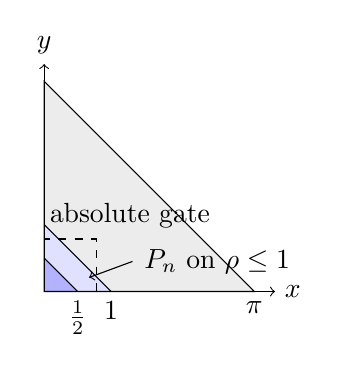
\begin{tikzpicture}[scale=0.85]
 \fill[gray!15] (0,1)--(1,0)--(3.14,0)--(0,3.14)--cycle;
 \fill[blue!12] (0,.5)--(.5,0)--(1,0)--(0,1)--cycle;
 \fill[blue!30] (0,0)--(.5,0)--(0,.5)--cycle;
 \draw (0,0)--(3.14,0)--(0,3.14)--cycle;
 \draw (.5,0)--(0,.5) (1,0)--(0,1);
 \draw[dashed] (0,0) rectangle (.7854,.7854);
 \draw[->] (0,0)--(3.45,0) node[right] {$x$};
 \draw[->] (0,0)--(0,3.4) node[above] {$y$};
 \node[below] at (.5,0) {$\frac12$};
 \node[below] at (1,0) {$1$};
 \node[below] at (3.14,0) {$\pi$};
 \node at (1.28,1.14) {absolute gate};
 \node[anchor=west] at (1.35,.45) {$P_n$ on $\rho\leq1$};
 \draw[->] (1.32,.45)--(.67,.21);
\end{tikzpicture}
\caption{The folded phase triangle. On the darkest triangle a
noncorner chart uses $\Delta>1/20$ together with $P_n$.
On $1/2\leq\rho\leq1$, $P_n<0$ suffices; the absolute gate covers
$\rho\geq1$. In a corner chart the dashed $\pi/4$ square has a
separate descent estimate.}
\label{fig:phase-regions}
\end{figure}

\subsection{A completed comparison model}
\label{uc:model}

\paragraph{The task of the comparison model.}
The quantity to be estimated is a finite sum of absolute values of a
polynomial kernel. Its individual rows have two large cotangent peaks.
The height of each peak changes with the phase, and the overlap between
the peaks changes too. A useful approximation must keep both pieces of
information: the sizes of the peaks and the cancellation between them.
This subsection constructs such an approximation, denoted $M_\infty$.
Its coefficients come from completed infinite sums and integrals; its
degree dependence enters through $L=\log n$.

The next subsection compares this approximation with the actual finite
sum. We first estimate the model on the whole closed phase triangle,
including its edges. We then estimate the discrepancy using the actual
rows of the finite board. The final corner comparison will use a loss
of size $uL^2$, a smaller possible gain of size $uL$, and finite errors.
Keeping this hierarchy in view explains the many constants below.

A phase is an angular displacement within a mesh cell. After folding
signs, its coordinates are $x,y\geq0$. They retain different meanings
because the mesh sizes are $n$ and $m=n+1$. Increasing $x$ moves the
samples along a row, whereas increasing $y$ moves the row itself. The
region $x+y\leq\pi$ is a triangle in the $(x,y)$ plane. Its origin
corresponds to the exact corner value used for comparison.

Throughout the comparison argument $m=n+1$, $L=\log n$, $H=1+L$,
$H_n=\sum_{j=1}^n j^{-1}$, and
\[
 \begin{gathered}
 x=|\alpha|,\quad y=|\beta|,\quad \rho=x+y\leq\pi,\quad
 c_e=\cos(\rho/2),\quad c_d=\cos((x-y)/2),\\
 a=c_ec_d,\quad u=1-a,\quad z=(1-c_e)(1-c_d).
 \end{gathered}
\]
Also put $p=\sin x$, $q=\sin y$, $P=p+q$, and $d_+=(q-p)_+$.
Thus $a=(\cos x+\cos y)/2\geq0$ and $2-c_e-c_d=u+z$.

The identity for $a$ follows from
$2\cos A\cos B=\cos(A+B)+\cos(A-B)$ with
$A=(x+y)/2$, $B=(x-y)/2$. Thus $0\leq a\leq1$, $u\geq0$,
and both $c_e,c_d$ lie in $[0,1]$, so $z\geq0$. The relation involving
$z$ is the exact multiplication
\[
 (1-c_e)(1-c_d)=1-c_e-c_d+c_ec_d.
\]
It retains the connection between the two cosine losses. Taylor's
formula near zero gives the useful size guide
\[
 u=\frac{x^2+y^2}{4}+O(\rho^4),\qquad
 z=\frac{(x+y)^2(x-y)^2}{64}+O(\rho^6).
\]
The proof below uses exact inequalities.
Also $P=p+q\leq x+y=\rho$ by $\sin t\leq t$. The notation
$d_+=(q-p)_+$ means $\max(q-p,0)$; it identifies the surviving
central logarithmic coefficient.
The two mesh directions retain their original roles throughout.
For real $C,D$ and $0<e<\pi$, define the complete cancellation
\begin{align}\label{uc:cancellation}
 I(C,D,e)&=\int_0^\pi
 \{|C\cot t+D\cot(t+e)|-|C\cot t|-|D\cot(t+e)|\}\,dt,\notag\\
 J(v,s,e)&=I((v-s)/2,(v+s)/2,e).
\end{align}
Write $g(C,D;t)$ for this integrand, with the separation understood.
We integrate the combined integrand, whose pole limits are finite.
It is invariant under simultaneous coefficient reversal, exchange of
channels, and reflection of the separation.

\paragraph{What is being cancelled.}
For real $A,B$ the elementary identity
\[
 |A+B|-|A|-|B|=
 \begin{cases}0,&AB\geq0,\\-2\min(|A|,|B|),&AB<0\end{cases}
\]
explains the name cancellation. When the channels have opposite signs,
the smaller magnitude is lost from both sides of the triangle
inequality. For values $5$ and $-2$, for example, the cancellation is
$3-5-2=-4$. In particular $g\leq0$ everywhere it is defined.

Each separate integral of $|\cot t|$ through a pole diverges. The
combined expression behaves differently. Near $t=0$, if $C\ne0$, the
channel $C\cot t$ dominates the bounded channel $D\cot(t+e)$. On
each side the displayed identity reduces $g$ to either zero or
$-2|D\cot(t+e)|$, with finite one-sided limits. The argument at the
other pole is the same; if a coefficient vanishes, the complete
cancellation is zero. Thus $I$ integrates the combined locally bounded
expression. Splitting at its finitely many transitions gives ordinary
improper integrals with finite limits.

The coordinates $v,s$ express $C+D=v$ and $D-C=s$. For nonnegative
$v,s$ with $s\leq v$, the coefficients in $J$ have the same sign; for $s>v$ they have
opposite signs. A root below means an equality point of their channel
magnitudes. These points delimit the intervals on which one particular
cotangent supplies the smaller magnitude.

\begin{lemma}[Cancellation and root formulas]\label{uc:cancellation-lemma}
For $v,s\geq0$, $0<e\leq\pi/2$, write
\[
 J(v,s,e)=2(s-v)_+\log\sin e+R(v,s,e).
\]
Then $R\leq0$,
\begin{align}\label{uc:R-bounds}
 |R|&\leq\max(2v,s+v)\log2,
 &|R_s|&\leq\log\frac{v+s}{|v-s|},\\
 R_e&=\frac{2\{v\cos e-\sqrt{(v^2-s^2\sin^2e)_+}\}}{\sin e}
 &&(s>v),\qquad R_e=0\quad(s\leq v).\notag
\end{align}
The derivative in $s$ is used as a locally integrable bound at $s=v$.
If
\begin{equation}\label{uc:root-Z}
 E(v,s,e)=J(v,s,e)-2s\log\sin e,\qquad
 Z(v,s,e)=2\int_e^{\pi/2}
       \frac{\sqrt{(v^2-s^2\sin^2t)_+}}{\sin t}\,dt,
\end{equation}
then $E\leq Z$, with equality for $s\geq v$.
All complete formulas extend continuously through zero coefficients
and moving equality roots.
\end{lemma}
\begin{proof}
On a sign interval the integrand is $-2$ times the smaller absolute
channel, and its primitive is a linear combination of logarithms of
sines. For $s\leq v$, with $c=(v-s)/2$, $b=(v+s)/2$, this gives
$J=2\{c\log(c/v)+b\log(b/v)\}$. Logarithms appear because $(\log|\sin t|)'=\cot t$. On an interval
where the two channel signs and the identity of the smaller magnitude
are fixed, the cancellation is a fixed multiple of one cotangent. Its
primitive is therefore explicit. Adding these interval integrals gives
the displayed formulas.

For $v>0$ and $0\leq s\leq v$, set $r=c/v$. The expression just obtained becomes
\[
 J=2v\{r\log r+(1-r)\log(1-r)\},\qquad 0\leq r\leq\tfrac12.
\]
The bracket ranges from $-\log2$ to zero, as follows by differentiating
it twice or by elementary convexity. This proves the sign and the
$2v\log2$ bound in this regime. The limit $r\log r\to0$ at zero
supplies the coefficient-zero convention. At $v=s=0$ the complete
cancellation is zero directly, in agreement with continuity.

For $s>v$, put
$c=(s-v)/2$, $b=(s+v)/2$. If $s\sin e\geq v$, integration gives
$J=2s\log\sin e$. Otherwise the equality roots satisfy
$\sin(2t+e)=s\sin e/v$. With
$t_1=(\arcsin(s\sin e/v)-e)/2$, the result is
\[
 J=2s\log\sin e+2\left\{
 b\log\frac{\cos t_1}{\sin(t_1+e)}
 -c\log\frac{\cos(t_1+e)}{\sin t_1}\right\}.
\]
For opposite signs an equality on the relevant sign interval reads
$c\cot t=b\cot(t+e)$. Multiplication by the sine factors and the
addition formulas give
\[
 (b-c)\sin(2t+e)=(b+c)\sin e.
\]
Here $b-c=v$ and $b+c=s$, yielding the stated root equation. Its
right side can be reached only when $s\sin e\leq v$. At strict
inequality there are two equality roots; at equality they merge; beyond
that threshold the extra root interval disappears. The square root in
$R_e$ arises from the cosine of the angle in this equation.

The explicit term $2(s-v)_+\log\sin e$ carries the singular behavior
as the separation shrinks. The remainder $R$ stays bounded in terms of
the coefficient sizes. Individual logarithms in the root formula may
look singular as a root or coefficient tends to zero. Their multiplying
coefficients make the complete expressions converge.

\paragraph{The actual integration intervals.}
Here is a way to reproduce the formulas without guessing a primitive
for the absolute value. Assume first $0<s<v$, put
$\theta=\arcsin((s/v)\sin e)$, and set
$y_0=(e-\theta)/2$, $y_1=(e+\theta)/2$. The cotangents have
opposite signs only on $(\pi/2-e,\pi/2)$ and $(\pi-e,\pi)$.
Use $t=\pi/2-u$ in the first and $t=\pi-r$ in the second.
The positive quantity whose integral is multiplied by $-2$ is
\[
\begin{array}{c|c|c}
 \text{variable}&\text{range}&\text{smaller channel magnitude}\\ \hline
 u&0<u<y_1&c\tan u\\
 u&y_1<u<e&b\tan(e-u)\\
 r&0<r<y_0&b\cot(e-r)\\
 r&y_0<r<e&c\cot r.
\end{array}
\]
The first crossing solves $c\tan u=b\tan(e-u)$ and the second
$c\cot r=b\cot(e-r)$. The addition formulas give precisely $y_1$
and $y_0$. Since $\int\tan u\,du=-\log\cos u$, adding the four
integrals gives
\[
 J=-2v\log\sin e+
 2c\log(\sin y_0\cos y_1)+2b\log(\sin y_1\cos y_0).
\]
Now
$\sin y_0\cos y_1=(\sin e-\sin\theta)/2=c\sin e/v$ and
$\sin y_1\cos y_0=b\sin e/v$. Substitution cancels the logarithms
of $\sin e$, leaving the entropy formula. The cases $s=0$ and $s=v$
follow by taking the stated continuous limits.

For $s>v$, the coefficients are $(-c,b)$. Cancellation occurs on
$(0,\pi/2-e)$ and $(\pi/2,\pi-e)$, where the cotangents have the
same sign. On the second interval the smaller magnitude is always
$c|\cot t|$, and its contribution to $J$ is $2c\log\sin e$.
On the first interval the smaller magnitude is $b\cot(t+e)$ unless
there are equality roots. If there are none, its contribution is
$2b\log\sin e$, proving $J=2s\log\sin e$. If there are roots,
write $t_2=(\pi-\theta-e)/2$ with
$\theta=\arcsin(s\sin e/v)$; then
\[
 -\tfrac12 J_{\rm first}
 =b\int_0^{t_1}\cot(t+e)dt
  +c\int_{t_1}^{t_2}\cot t\,dt
  +b\int_{t_2}^{\pi/2-e}\cot(t+e)dt.
\]
Evaluating each integral at its two endpoints and using
$t_2=\pi/2-t_1-e$ gives the root formula above. This also identifies
the intervals that disappear when the roots merge.

\paragraph{Differentiating the remainder explicitly.}
Put $D_*=(v^2-s^2\sin^2e)_+^{1/2}$. For $s<v$ the entropy
formula gives
\[
 R_s=\log\frac{v+s}{v-s},\qquad R_e=0.
\]
For $s>v$, differentiation of the three definite integrals just written
cancels their moving-boundary terms. In the root regime the remaining
terms simplify to
\[
 R_s=\log\frac{s\cos e-D_*}{s\cos e+D_*},\qquad
 R_e=\frac{2(v\cos e-D_*)}{\sin e}.
\]
In the regime $s\sin e\geq v$, the explicit formula instead gives
$R=2v\log\sin e$, so $R_s=0$ and $R_e=2v\cot e$. For $s>v$,
$0\leq D_*\leq v\cos e$; consequently the root-regime quotient
lies between $(s-v)/(s+v)$ and one. This proves the stated bound for
$|R_s|$ and also $0\leq R_e\leq2v\cot e$.

For the size bound, the endpoint value for $s>v$ has $b=c+v$ and
can be written
\[
 R(v,s,0)=2b\left\{\frac cb\log\frac cb+
                         \frac vb\log\frac vb\right\}.
\]
The bracket is between $-\log2$ and zero. Monotonicity in $e$ and
the value zero at $\pi/2$ thus give $-(s+v)\log2\leq R\leq0$.
For $s\leq v$ the earlier entropy calculation gives
$-2v\log2\leq R\leq0$. These are exactly the two parts of the
single bound in the lemma.

These expressions have matching limits at every threshold, using
$0\log0=0$. Differentiation gives \eqref{uc:R-bounds}; the moving
endpoint terms cancel because the channel magnitudes agree there.
The endpoint cancellation under differentiation can be checked with
the Leibniz rule. If two integrands $h_1,h_2$ meet at a moving root
$r(\lambda)$, their endpoint contributions have sum
\[
 \{h_1(r(\lambda),\lambda)-h_2(r(\lambda),\lambda)\}r'(\lambda)=0.
\]
The equality defining the root is precisely what makes the bracket zero.
The logarithmic bound for $R_s$ is locally integrable at $s=v$, since
$\int_0^\eta|\log t|dt=\eta(1-\log\eta)$ for $\eta<1$.
Later parameter estimates integrate this locally integrable bound over
a range of $s$.

For $s>v$, $R$ increases from
$2(c\log c+v\log v-b\log b)$ at $e=0$ to zero at $e=\pi/2$.
These endpoints, and the entropy expression for $s\leq v$, give its
sign and size bounds. Subtracting $2s\log\sin e$ gives derivative
$-2\sqrt{(v^2-s^2\sin^2e)_+}/\sin e$ in the root regime and zero
beyond its threshold. Integration from that threshold proves $E=Z$
for $s\geq v$. For $s<v$, $J\leq0$ and
$\sqrt{v^2-s^2\sin^2t}\geq s\cos t$, whence
$Z\geq-2s\log\sin e\geq E$. The case $v=0$ is direct.

The advantage of $Z$ is its nonnegative integrand and explicit
support:
\[
 \sqrt{(v^2-s^2\sin^2t)_+}>0\quad\Longleftrightarrow\quad s\sin t<v.
\]
For $s\geq v$, integrating the derivative from the threshold where
both sides vanish proves $E=Z$. For $s<v$, the comparison in the
proof uses $v^2-s^2\sin^2t\geq s^2\cos^2t$, and hence
\[
 Z\geq2s\int_e^{\pi/2}\cot t\,dt=-2s\log\sin e\geq E.
\]
Nonnegative root integrals can be reordered by Tonelli's theorem: a
nonnegative double integral has the same value in either order, even
before its finiteness is established. That fact will let us estimate two
central root contributions together.
\end{proof}

\paragraph{From reciprocal sums to a scalar profile.}
Near a pole an absolute cotangent behaves like the reciprocal of its
distance. A mesh samples both sides of the pole. The parameter
$t\in(0,1)$ gives its fractional position between consecutive samples,
with distances $t,1-t,1+t,2-t,\ldots$. Pairing these distances and
subtracting their common harmonic growth leaves $\mathcal C$. For
fixed $t$,
\[
 \frac1{k+t}+\frac1{k+1-t}-\frac2k=O(k^{-2}),
\]
so the series converges. At $t=0$ or $1$ a reciprocal term diverges,
but the sine factor in $\Phi$ removes this pole:
$\sin(\pi t)/(\pi t)\to1$. The weighted profile fits the polynomial
rows because the corresponding cotangent coefficient contains the same
sine factor. Periodic extension joins its finite endpoint values.
Centering at $t=1/2$ gives the even function $f$; its joined endpoint
$w=\pi$ modulo $2\pi$ is the cusp, where its left and right slopes
differ.

The scalar reciprocal pair and its continuous periodic profile are
\begin{align}\label{uc:scalar-definitions}
 \mathcal C(t)&=2\gamma+\frac1t+\frac1{1-t}
 +\sum_{k\geq1}\left\{\frac1{k+t}+\frac1{k+1-t}-\frac2k\right\},
 \notag\\
 C_0&=\mathcal C(1/2)=2\gamma+4\log2,\notag\\
 \Phi(t)&=\frac{\sin\pi t}{\pi}\{\mathcal C(t)-2\log\pi\},
 \quad\Phi(0)=\Phi(1)=1,\notag\\
 f(w)=\Phi(1/2+w/(2\pi)).
\end{align}
Extend $\Phi$ with period one. Then $f$ is even with period $2\pi$.
We use $\psi(t)=-\gamma+\sum_{k\geq0}\{(k+1)^{-1}-(k+t)^{-1}\}$,
so $\mathcal C(t)=-\psi(t)-\psi(1-t)$.

\paragraph{A derivative measure and a finite part.}
A Lipschitz function satisfies $|f(w)-f(v)|\leq K|w-v|$. Its first
derivative can still jump. Here its ordinary second derivative is $g$
away from the cusp, and $f'$ has a downward jump of size $J_0$ at the
joined endpoint. The notation $df'=g(w)\,dw-J_0\delta_\pi$ includes
both changes. Integrating this measure over an interval gives the
change of $f'$ across that interval; the point mass $\delta_\pi$
contributes one if the cusp lies inside. Total variation adds the
absolute sizes of all changes. On a circle the joined endpoint must
be counted once.

The kernel $1/(2\sin(t/2))$ has reciprocal singularities at both
ends of $[0,2\pi]$. Its integral against $f(w+t)$ diverges like
$-2f(w)\log\epsilon$. The counterterm in $H$ subtracts that known
divergence, keeping a finite constant. This prescription is called a
finite part. A Cauchy principal value, by comparison, takes matched
cutoffs on opposite sides to cancel signed singularities. Here the
explicit logarithmic counterterm and its normalization by $\pi$
define the value completely. They must be carried together when the
constant is compared at different phases.

In the series estimates, $\zeta(s)=\sum_{k\geq1}k^{-s}$ for $s>1$
denotes the convergent reciprocal-power sum.

\begin{lemma}[The scalar maximum, including its cusp]\label{uc:scalar-maximum}
The function $f$ is Lipschitz, $f'$ has bounded variation on the circle,
and, for its ordinary second derivative $g$ on $(-\pi,\pi)$,
\begin{equation}\label{uc:scalar-bounds}
 \begin{gathered}
 \frac12<f\leq1,\quad \operatorname{Lip}(f)<2,\quad
 |g|<1,\quad |f'''|<13/20,\quad
 \operatorname{Var}_{\rm per}f'<4,\\
 df'=g(w)\,dw-J_0\delta_\pi\leq\frac3{\pi^2}\,dw,
 \quad J_0=\frac{2(\log\pi-\gamma)}\pi>\frac1\pi.
 \end{gathered}
\end{equation}
The endpoint atom is counted once. The finite part
\begin{equation}\label{uc:H}
 H(w)=\frac1\pi\lim_{\epsilon\downarrow0}
 \left\{\int_\epsilon^{2\pi-\epsilon}
 \frac{f(w+t)}{2\sin(t/2)}\,dt+2f(w)\log\frac\epsilon\pi\right\}
\end{equation}
satisfies $H(w)\leq H_0:=H(0)$ for all real $w$.
\end{lemma}
\begin{proof}
On $0<t\leq1/2$ the defining series becomes
\[
 \mathcal C(t)=t^{-1}+2\gamma+Q(t),\qquad
 Q(t)=2\sum_{j\geq1}\zeta(2j+1)t^{2j}.
\]
The expansion of $Q$ follows by geometric series. For example,
\[
 \frac1{k+t}+\frac1{k-t}-\frac2k
 =\frac{2t^2}{k(k^2-t^2)}
 =2\sum_{j\geq1}\frac{t^{2j}}{k^{2j+1}}.
\]
For $t\leq1/2$, uniform geometric majorants justify summing and
differentiating the needed series. Summing over $k$ gives the zeta
values. Integral comparison bounds a decreasing positive sum by
integrals over adjacent unit intervals. This supplies simple rational
bounds for the zeta values and their tails. The constants used here
are deliberately broad enough to make subsequent error estimates easy
to check.

Integral comparison gives $\zeta(3)<5/4$, hence
$Q\leq4t^2$, $Q'\leq5t/(1-t^2)^2\leq(32/3)t$, and
$Q''\leq Q''(1/2)=28\zeta(3)-16<19$
(the weaker absolute bound $608/27$ is also convenient).
With $k=2\gamma-2\log\pi$,
\[
 \Phi(t)=\frac{\sin\pi t}{\pi t}
             +k\frac{\sin\pi t}\pi+Q(t)\frac{\sin\pi t}\pi.
\]
Since $k+Q<0$, this is at most one. For the lower bound, put
$k_0=C_0-2\log\pi$ and $c_s=\cos(\pi s/2)$. Reciprocal pairing gives
\begin{equation}\label{uc:f-series}
 f(w)=\frac{\cos(w/2)}\pi
 \left\{k_0+4w^2\sum_{\ell\geq1,\ \ell\ {\rm odd}}
       \frac1{\ell(\ell^2\pi^2-w^2)}\right\},\quad |w|<\pi.
\end{equation}
The inequality $c_s\geq(3/4)(1-s^2)$ follows by differentiating
$\sin(\pi r/2)-(3/4)r(2-r)$, $r=1-s$: its second derivative
changes sign once, and its first derivative ends at zero. Keeping
$\ell=1$ in \eqref{uc:f-series}, and using
$1-c_s\leq\pi^2s^2/8$, $k_0<2$, $\pi^2<10$, gives
$\pi f(\pi s)\geq c_sk_0+4c_ss^2/(1-s^2)\geq k_0$.
The elementary bounds $\gamma>23/40$, $\log2>69/100$,
$\log\pi<23/20$ give $k_0>161/100>\pi/2$.

The centered reciprocal series also explains the lower bound. Its
$\ell=1$ term is positive and becomes large near the endpoint, while
the prefactor $c_s=\cos(\pi s/2)$ removes its pole. In detail,
\[
 c_sk_0+\frac{4c_ss^2}{1-s^2}-k_0
 \geq-\frac{k_0\pi^2s^2}{8}+3s^2\geq0,
\]
using $c_s\geq(3/4)(1-s^2)$, $k_0<2$, and $\pi^2<10$.
Thus $f(w)\geq k_0/\pi>1/2$, with endpoint values supplied by
continuity. The upper bound comes from the endpoint representation of
$\Phi$. Positivity will matter when weighted reciprocal estimates
are multiplied later.

\paragraph{A table for the scalar derivative bounds.}
The reciprocal formula for $Q$ and its first two derivatives is
\[
 \begin{aligned}
 Q(t)&=2t^2\sum_{k\geq1}\frac1{k(k^2-t^2)},\\
 Q'(t)&=4t\sum_{k\geq1}\frac{k}{(k^2-t^2)^2},\\
 Q''(t)&=4\sum_{k\geq1}\frac{k}{(k^2-t^2)^2}
           +16t^2\sum_{k\geq1}\frac{k}{(k^2-t^2)^3}.
 \end{aligned}
\]
On $t\leq1/2$, $k^2-t^2\geq3k^2/4$. Using
$\sum k^{-3}<3/2$ and $\sum k^{-5}<5/4$ in the last line gives
$Q''\leq32/3+320/27=608/27$. The sharper endpoint value follows
by differentiating the reciprocal pair twice:
$\mathcal C''(1/2)=4\sum_{k\geq0}(k+1/2)^{-3}=28\zeta(3)$.
The second derivative of $1/t$ there is $16$, so subtracting it gives
$Q''(1/2)=28\zeta(3)-16$. Positivity of the power-series coefficients
makes $Q''$ increasing. For a fully rational estimate,
\[
 \zeta(3)\leq1+\frac18+\frac1{27}+\int_3^\infty r^{-3}dr<\frac54.
\]
Summing the geometric series then gives
$Q\leq(5/2)t^2/(1-t^2)\leq4t^2$ and
$Q'\leq5t/(1-t^2)^2\leq16/3$. Also $k<-1$, from
$\gamma<3/5$, $\log\pi>11/10$, while $Q\leq1$; hence $k+Q<0$
as used for the upper bound on $\Phi$.

Let $T(t)=\sin(\pi t)/(\pi t)=\int_0^1\cos(\pi tr)dr$.
Differentiating this integral bounds $|T'|$ by $\pi/2<2$ and
$|T''|$ by $\pi^2/3<10/3$. The other differentiated terms of
$\Phi=T+k\sin(\pi t)/\pi+Q\sin(\pi t)/\pi$ give
\[
\begin{array}{c|c}
 \text{term in }\Phi''&\text{absolute upper bound}\\ \hline
 T''&10/3\\
 -k\pi\sin(\pi t)&10\\
 Q''\sin(\pi t)/\pi&608/81\\
 2Q'\cos(\pi t)&32/3\\
 -\pi Q\sin(\pi t)&10/3.
\end{array}
\]
Their sum is $2822/81<35$. Similarly the first derivatives of the
three summands are bounded respectively by $2$, $5$, and $4$:
for the last use $Q'/\pi+Q<16/9+1<4$. The factor $1/(2\pi)$
in a $w$ derivative then gives the claimed Lipschitz constant.

For the upper curvature bound retain signs. The sinc integral and
$\cos r\geq1-r^2/2$ give
\[
 T''\leq-\pi^2\left(\frac13-\frac{\pi^2}{40}\right).
\]
Moreover $\cos\pi t\leq\pi(1/2-t)$, and
\[
 3+34t^2+3t^4-20t
 \geq34(t-5/17)^2+1/17>0.
\]
Thus $2Q'\cos\pi t\leq3\pi/4$. Dropping the nonpositive last
term in the table and using $-k<5/4$ yields
$\Phi''\leq-\pi^2/12+2\pi+19/\pi<12$.
The earlier sine comparison can likewise be checked explicitly:
for $h(r)=\sin(\pi r/2)-(3/4)r(2-r)$, $h(0)=0$, $h'(1)=0$,
and $h''$ decreases through zero once. Therefore $h'$ first increases
and then decreases to zero, staying positive, and $h\geq0$.

Differentiating the three terms of $\Phi$ bounds their first
 derivatives by $2,5,4$, respectively. Their five second-derivative
contributions have absolute bounds
$10/3,10,608/81,32/3,10/3$, whose sum is less than $35$.
Thus $\operatorname{Lip}(f)<6/\pi<2$ and $|g|<35/(4\pi^2)<1$.
For the one-sided bound use
\[
 \left(\frac{\sin\pi t}{\pi t}\right)''
 \leq-\pi^2(1/3-\pi^2/40)\leq-\pi^2/12,
 \quad \frac{t(1/2-t)}{(1-t^2)^2}\leq\frac3{40}.
\]
The latter follows from $3+34t^2+3t^4-20t>0$.
Since $-k<5/4$, differentiation gives
$\Phi''\leq-\pi^2/12+2\pi+19/\pi<12$.
The absolute second-derivative bound and the upper curvature bound
serve different purposes. The absolute bound controls ordinary changes;
the upper bound retains favorable negative terms. The scaling
$t=1/2+w/(2\pi)$ divides second derivatives by $4\pi^2$, so
$\Phi''<12$ gives $g<3/\pi^2$. A downward jump only strengthens
this upper bound. Concretely, for a nonnegative continuous periodic
function $\chi$ the measure inequality says
\[
 \int\chi\,df'\leq\frac3{\pi^2}\int\chi(w)\,dw.
\]
The total change of a periodic derivative is zero. Its positive and
negative masses therefore have equal magnitudes, so bounding its
positive mass bounds its total variation by twice that amount.

At an integer $\Phi'$ has jump $2k<0$; reflection matches its
ordinary derivative at the half integer. Scaling proves the measure
bound in \eqref{uc:scalar-bounds}, including the stated atom.
The positive mass of $df'$ is at most $6/\pi$, its total mass is
zero, and therefore its variation is at most $12/\pi<4$.

For the remaining derivative facts an endpoint-cancelled formula is
useful:
\begin{equation}\label{uc:f-integral}
 f(w)=f(0)\cos(w/2)+2\int_0^{1/2}
       \frac{\cos(wt)-\cos(w/2)}{\cos\pi t}\,dt,\qquad |w|\leq\pi.
\end{equation}
At $t=1/2$ the numerator in this integral vanishes along with
$\cos\pi t$. The mean value theorem bounds
$|\cos(wt)-\cos(w/2)|$ by $|w|(1/2-t)$, while
$\cos\pi t\geq2(1/2-t)$. The quotient is consequently bounded.
Each of its first three differentiated numerators in $w$ still
vanishes at $t=1/2$. The same argument, on the compact range
$|w|\leq\pi$, supplies integrable majorants for those derivatives.

The factors $r^{2j+1}$ below first make the trigonometric series
absolutely convergent for $r<1$. The sum may then be integrated term
by term. Taking $r\uparrow1$ is justified by the displayed common
majorant and dominated convergence: pointwise convergence under one
integrable bound permits passage to the limit in the integral. This
proves the formula at the joined endpoints as well as in the interior.

To derive it, integrate the numerator against $\cos((2j+1)\pi t)$;
the result is
$(-1)^j\cos(w/2)w^2/[(2j+1)\pi((2j+1)^2\pi^2-w^2)]$.
The Abel sum of the kernels is
\[
 \sum_{j\geq0}(-1)^jr^{2j+1}\cos((2j+1)\pi t)
 =\frac{r(1+r^2)\cos\pi t}{(1-r^2)^2+4r^2\cos^2\pi t}
 \longrightarrow\frac1{2\cos\pi t}.
\]
For $r\geq1/2$ it is bounded by $5/(8\cos\pi t)$, while the
numerator is $O(1/2-t)$ and $\cos\pi t\geq2(1/2-t)$.
Dominated convergence proves \eqref{uc:f-integral}, including its
endpoints, and permits three derivatives because each differentiated
numerator also vanishes at $t=1/2$. In particular
\[
 f'''(w)=\frac{f(0)}8\sin(w/2)
 +2\int_0^{1/2}\frac{t^3\sin(tw)-\sin(w/2)/8}{\cos\pi t}\,dt.
\]
The numerator's $t$ derivative has magnitude at most
$3/4+\pi/8<23/20$, giving $|f'''|<23/40+3/40=13/20$.
For $0<w\leq\pi$, monotonicity of $r\cot r$ gives
$\sin(tw)/\sin(w/2)\leq\sin\pi t$. Since $f(0)<3/5$, split
$[0,1/2]$ at $1/4,3/8$, use respectively $\sin\pi t\leq(22/7)t$
and $t^3\sin\pi t\leq27/512$, and discard the negative last part.
This yields
\[
 \frac{f'''(w)}{\sin(w/2)}
 <\frac3{40}+\frac{44}{35\cdot1024}-\frac1{16}-\frac{37}{2048}
 =-\frac{311}{71680}<0.
\]
Consequently $g$ is even and decreases radially.

The sine-ratio step follows from ordinary differentiation. For fixed
$0<t<1/2$ set $R_t(w)=\sin(tw)/\sin(w/2)$. On $0<w<\pi$,
\[
 (\log R_t)'=t\cot(tw)-\tfrac12\cot(w/2)>0,
\]
because $(r\cot r)'=(\sin r\cos r-r)/\sin^2r<0$ for
$0<r\leq\pi/2$. Hence $R_t(w)\leq R_t(\pi)=\sin\pi t$.
After this substitution the integral bounding
$f'''(w)/\sin(w/2)$ has negative numerator
$t^3\sin\pi t-1/8$. Dividing by $\cos\pi t\leq1$ makes that
negative number smaller. Thus the first two interval contributions are
\[
 \begin{aligned}
 2\int_0^{1/4}\frac{t^3\sin\pi t-1/8}{\cos\pi t}dt
 &\leq2\int_0^{1/4}\left(\frac{22}{7}t^4-\frac18\right)dt
 =\frac{44}{35\cdot1024}-\frac1{16},\\
 2\int_{1/4}^{3/8}\frac{t^3\sin\pi t-1/8}{\cos\pi t}dt
 &\leq2\left(\frac38-\frac14\right)
                    \left(\frac{27}{512}-\frac18\right)
 =-\frac{37}{2048}.
 \end{aligned}
\]
The last interval contributes a negative amount, which may be dropped
for an upper bound. Together with $f(0)/8<3/40$, these evaluated
integrals give exactly the rational negative coefficient above.

The sign of the third derivative says that $g=f''$ decreases as
$|w|$ increases from zero to $\pi$. This is the meaning of radially
decreasing on the circle. It is the order property needed for the
finite-part maximum. Pairing the endpoints removes the logarithmic
divergence directly: the Lipschitz bound gives
\[
 |f(w+t)+f(w-t)-2f(w)|\leq2\operatorname{Lip}(f)t,
\]
and $2\sin(t/2)$ is comparable to $t$ on $[0,\pi]$. Thus the next
quotient is integrable, including at a cusp. At an ordinary smooth
point its numerator is even $O(t^2)$, but the weaker uniform estimate
is sufficient.

Pairing endpoints in \eqref{uc:H} gives the absolutely convergent
formula
\[
 H(w)=\lambda_0f(w)+\frac1\pi\int_0^\pi
 \frac{f(w+t)+f(w-t)-2f(w)}{2\sin(t/2)}\,dt,
 \qquad \lambda_0=\frac2\pi\log\frac4\pi<\frac1{2\pi}.
\]
The bound follows from $\pi>25/8$ and $e^{1/4}>32/25$.
Set $W(t)=\int_{|t|}^\pi\log\cot(s/4)\,ds$ on the circle.
It is bounded, nonnegative and radially decreasing. Integrating the
triangular-kernel representation of the second difference against
$df'$ gives
\[
 H(w)=\lambda_0f(w)+\frac1\pi\int_{-\pi}^{\pi}W(t)g(w+t)\,dt
                  -\frac{J_0}\pi W(\pi-|w|),\quad |w|\leq\pi.
\]
For a smooth function the second-difference identity is
\[
 f(w+t)+f(w-t)-2f(w)
 =\int_{-t}^{t}(t-|s|)f''(w+s)\,ds.
\]
It follows by integrating the derivative twice. For a derivative of
bounded variation the same identity holds with its finite measure
$df'$ in place of $f''\,ds$; the triangular weight is continuous.
Integrating this identity against the reciprocal-sine kernel gives
$W$. Its boundedness and the finite total variation justify the
interchange of the two integrals. The ordinary curvature yields the
convolution term; the cusp yields the separate negative term.

The layer-cake argument can be expressed using indicator functions:
$h(t)=\int_0^\infty\mathbf1_{h(t)>r}dr$ for $h\geq0$.
For an even radially decreasing function each superlevel set is a
centered arc. A product integral becomes an integral of lengths of
intersections of two arcs. Each intersection is at most the length of
the smaller arc, and equal centers attain that value. Translation can
therefore only decrease the centered convolution. Subtracting the
minimum of $g$ makes it nonnegative without changing which translate
maximizes its convolution with $W$.

Fubini is valid against the finite variation measure; $W(\pi)=0$
counts the atom only once. Subtract the minimum of $g$ to make it
nonnegative. Layer cake reduces its convolution with $W$ to lengths
of intersections of two centered circular arcs; a translate cannot
increase such a length. The convolution is therefore largest at zero.
The measure bound implies $f(w)-f(0)\leq3w^2/(2\pi^2)$, and
$W(\pi-|w|)\geq w^2/4$, since the derivative of
$\log\cot((\pi-s)/4)$ is $1/(2\cos(s/2))\geq1/2$.
Thus $H(w)-H_0\leq-(\pi-3)w^2/(4\pi^3)\leq0$.
Continuity and periodicity include the closed endpoints.

The final quadratic comparison also follows by integration. Since
$f'(0)=0$, the upper measure bound gives
$f(w)-f(0)\leq3w^2/(2\pi^2)$. The estimate for $W$ is
\[
 W(\pi-w)=\int_0^w\log\cot((\pi-s)/4)\,ds\geq w^2/4,
 \qquad 0\leq w\leq\pi.
\]
With $\lambda_0<1/(2\pi)$ and $J_0>1/\pi$, these yield the
negative coefficient $(3-\pi)/(4\pi^3)$ in $H(w)-H_0$.
This explains how the finite part $H$ is largest at zero although
$f$ itself reaches its largest value at the joined endpoint: curvature
and the cusp contribution enter the finite part as well.

The weight $W$ can be obtained explicitly from the triangular
identity. For a curvature contribution at displacement $s\geq0$,
its integrated weight is
\[
 K(s)=\int_s^\pi\frac{t-s}{2\sin(t/2)}dt.
\]
Differentiating in $s$ gives
$K'(s)=-\int_s^\pi dt/(2\sin(t/2))=-\log\cot(s/4)$,
and $K(\pi)=0$. Therefore
$K(s)=\int_s^\pi\log\cot(t/4)dt=W(s)$. This evaluates the
kernel produced by the change of integration order and explains the
specific logarithm in the convolution formula.
\end{proof}

\paragraph{The row profile.}
The variable $v$ gives the angular position of a row. The coefficients
$C(v),D(v)$ are its two cotangent amplitudes. Near an endpoint they
contain a term proportional to $a/v$. Averaging a cotangent peak along
one mesh produces a logarithm, and summing such row averages over the
other mesh produces another logarithm. This accounts for the leading
$L^2$ term of the completed model.

The coefficient $A(v)$ records the $L$ part of a single-row average.
Its constant part $\mathcal B(v)$ combines the two weighted scalar
pole profiles with their complete cancellation. An approximation is
called completed here because it includes the full infinite endpoint
reference and a specified subtracted integral for the constant. This
fixes the constant term as well as the leading growth. A bounded but
unspecified constant error would be too large for the strict corner
comparison later in the argument.

For $0<v<2\pi$ define the row coefficients and profile
\begin{align}\label{uc:row-profile}
 C(v)&=(p-q-2a\cot(v/2))/4,\quad D(v)=(p+q+2a\cot(v/2))/4,\notag\\
 \eta_-(v)&=\tfrac12+(x-y+v)/(2\pi),\quad
 \eta_+(v)=\tfrac12+(x+y-v)/(2\pi),\notag\\
 A(v)&=2(|C(v)|+|D(v)|)/\pi,\notag\\
 \mathcal B(v)&=\frac{c_e\Phi(\eta_-(v))+c_d\Phi(\eta_+(v))}
                         {2\sin(v/2)}+\frac{I(C(v),D(v),v)}\pi.
\end{align}
Write $\mathcal H(L,v)=A(v)L+\mathcal B(v)$ and
$U_0=c_ef(x-y)+c_df(x+y)$, $B_0=4a/\pi^2$,
$D_0=U_0/\pi+B_0\log\pi$. The completed model is
\begin{equation}\label{uc:completed-model}
 \begin{gathered}
 M_\infty(x,y,L)=\frac{4a}{\pi^2}L^2+b_{\rm full}L+C_\infty,\quad
 b_{\rm full}=\frac{2U_0}\pi+
 \frac{8a\log2+4a\log a+2(xp+yq)}{\pi^2},\\
 E_\infty=\frac a3+
 \frac{a}{\pi^2}\mathcal C(1/2+(x-y)/(2\pi))
                         \mathcal C(1/2+(x+y)/(2\pi)),\\
 C_\infty=E_\infty+\lim_{\epsilon\downarrow0}
 \left\{B_0\log^2\frac\epsilon\pi+2D_0\log\frac\epsilon\pi
            +\frac1\pi\int_\epsilon^{2\pi-\epsilon}\mathcal B(v)\,dv\right\}.
 \end{gathered}
\end{equation}
Weighted endpoint products and $a\log a$ have their continuous values.

The endpoint convention is visible in one variable:
$\mathcal C(t)\sim1/t$ and $\sin\pi t\sim\pi t$ as $t\downarrow0$,
so the weighted product tends to $\pi$. In $E_\infty$ the factor
$a=c_ec_d$ supplies the two needed cosine weights. The complete
product stays finite on an edge where an unweighted reciprocal factor
diverges. Similarly $a\log a\to0$ as $a\downarrow0$.

Two counterterms occur because the endpoint profile has both a
reciprocal and a logarithmic-reciprocal part. On each folded side its
leading expression is
\[
 \frac{U_0}{t}+\frac{4a}{\pi}\frac{\log t}{t},
\]
whose primitives are $U_0\log t$ and $(2a/\pi)\log^2t$.
There are two sides, and the integral has an outer factor $1/\pi$.
This gives the coefficients $B_0$ and $2D_0$ after changing the
normalization from $\log\epsilon$ to $\log(\epsilon/\pi)$.
In particular $B_0\log\pi$ inside $D_0$ is the cross term from
this change. The pieces of the finite part must be kept together
because this normalization fixes its constant.

At the origin, $a=c_e=c_d=1$, $p=q=0$, and
$U_0=2f(0)=2k_0/\pi$. Substitution in the model's linear coefficient
gives
\[
 b_{\rm full}(0)=\frac{4k_0+8\log2}{\pi^2}
 =\frac{8\{\gamma+\log(8/\pi)\}}{\pi^2}=b_c.
\]
This check ties the completed row normalization to the corner
normalization used later.

The limit exists uniformly on the closed phase triangle. We give an
explicit envelope, also needed for the finite mesh. For either folded
side $v_L(t)=t$, $v_R(t)=2\pi-t$, $0<t\leq\pi/4$,
\begin{equation}\label{uc:endpoint-envelope}
 \left|\mathcal B(v_s(t))-
       \frac{U_0+(4a/\pi)\log t}{t}\right|
 \leq7+\frac P\pi\left(3+2\log\frac{4\pi}{t}\right).
\end{equation}
\paragraph{Uniform control near an endpoint.}
A limit is uniform in phase if one cutoff works for every point of
the closed triangle. This is needed because a maximizing phase may
move with $n$ or approach an edge. The envelope just displayed gives
this control after the explicit endpoint singularity is removed. Its
right side is integrable, since
\[
 \int_0^\eta\log(A/t)\,dt=\eta\{1+\log(A/\eta)\}\longrightarrow0.
\]
The omitted short intervals therefore have contributions tending to
zero uniformly in phase. This proves that the completed constants
are uniformly Cauchy and later bounds the mesh intervals that contain
no retained sample.

The reference coefficients $(-w,w)$ preserve the large endpoint
amplitudes. Their cancellation is explicitly integrable. The phase
adds coefficient displacements of size at most $P/4$. Integrating a
bound involving the absolute cotangents over the whole interval would
lose finiteness at their poles. The proof first uses channel dominance
on short pole arcs and then uses the ordinary Lipschitz inequality for
absolute values on their complement.

To prove this, compare $I(C,D,t)$ with $I(-w,w,t)$, where
$w=a\cot(t/2)/2$ and each coefficient displacement is at most $P/4$.
For general displacements at most $\varepsilon$, remove pole arcs of
radius $t/8$. If $w\geq4\varepsilon$, the own channel dominates there
and the two cancellations differ by at most $8\varepsilon/7$ in
integral. If $w<4\varepsilon$, both complete cancellations are bounded
by twice the other channel, costing at most $72\varepsilon/7$.
On the complement their difference is at most
$2\varepsilon(|\cot z|+|\cot(z+t)|)$, whose integral is at most
$8\varepsilon\log(4\pi/t)$. Thus
\[
 |I(C,D,t)-I(-w,w,t)|\leq\varepsilon[11+8\log(4\pi/t)],
 \qquad I(-w,w,t)=4w\log\sin t.
\]
On the complement, changing each coefficient by at most $\varepsilon$
changes the complete cancellation by at most
$2\varepsilon(|\cot z|+|\cot(z+t)|)$, by two applications of
$||A|-|B||\leq|A-B|$. Deleting arcs of radius $t/8$ leaves a
logarithmic cotangent integral. On an arc, either the reference
coefficient is large enough to dominate the bounded other channel,
or all coefficients have size comparable to $\varepsilon$. This
explains the two cases $w\geq4\varepsilon$ and $w<4\varepsilon$
and their finite costs proportional to $\varepsilon$.

For the reference, the first lemma with $v=0$, $s=2w$ gives
$I(-w,w,t)=4w\log\sin t$. Replacing it by its singular part uses
$\cot(t/2)-2/t=O(t)$ and $\log(\sin t/t)=O(t^2)$.
Multiplication by the remaining reciprocal factor leaves integrable
errors of size $O(t(1+|\log t|))$. The numerator estimate below uses
the global Lipschitz bound for $f$, so it also works when a shifted
scalar argument crosses its cusp.

For the pole numerator $N_s$, $|N_s(t)-U_0|\leq12t/\pi$,
$|N_s|\leq8$. The sine chord gives a pole remainder at most
$6+\pi t/6$. Finally
$|2a\cot(t/2)\log\sin t-(4a/t)\log t|
\leq at(1+|\log t|)$. These estimates give \eqref{uc:endpoint-envelope}.
Its integrable right side makes the finite parts uniformly Cauchy.
The cancellation lemma bounds all central root transitions by an
integrable multiple of $1+|\log\sin t|$; hence their limits are
continuous in phase, including the axes and vertices.

On any truncated interval the complete cancellation depends
continuously on phase, including when equality roots merge. The first
lemma supplies continuous formulas and a common integrable bound.
Dominated convergence gives continuity there. The endpoint envelope
makes the rest uniformly small, proving continuity of the completed
constant on the closed triangle.

The next calculation independently checks the logarithmic coefficient.
The absolute coefficient sum is a piecewise maximum. Its transition
points can be found before integrating, and each piece has an elementary
primitive. Using $X=\max(x,y)$ and $Y=\min(x,y)$ organizes this scalar
calculation; the row roles of $x$ and $y$ are still retained in the
finite argument. At $a=0$ individual logarithmic primitives can look
singular, but the resulting expression has the specified continuous
$a\log a$ value. The integrable subtracted maximum provides the
justification for passage to that edge.

For clarity the logarithmic coefficient can be checked independently.
Put $X=\max(x,y)$, $Y=\min(x,y)$ and $T_t=2a\cot(t/2)$. Then
$\pi(A(t)+A(2\pi-t))$ is respectively
$2T_t$, $T_t+p+q$, $2\sin X$ on the intervals cut by
$\pi-X-Y$ and $\pi-X+Y$. Integrating with
$\int T_t\,dt=4a\log\sin(t/2)$ gives
\[
 \int_0^\pi\{A(t)+A(2\pi-t)-8a/(\pi t)\}\,dt
 =\{8a\log(2/\pi)+4a\log a+2(xp+yq)\}/\pi.
\]
Here is the piecewise integration. The identity
$|p-h|+|p+h|=2\max(p,|h|)$ gives
\[
 \pi A(t)=\max(p,q+T_t),\qquad
 \pi A(2\pi-t)=\max(p,|q-T_t|).
\]
Also $\sin X\geq\sin Y$, because
$\sin X-\sin Y=2\cos((X+Y)/2)\sin((X-Y)/2)\geq0$.
The changes of branch occur when $T_t=p+q$ and $T_t=|p-q|$.
The addition formulas put these respectively at
$t_1=\pi-X-Y$ and $t_2=\pi-X+Y$. First take $x+y<\pi$ and
$0<\epsilon<t_1$. Then, before subtracting
the reciprocal integral, the sum of the three pieces on $[\epsilon,\pi]$
is
\[
 \begin{aligned}
 &\pi\int_\epsilon^\pi\{A(t)+A(2\pi-t)\}dt\\
 &=2\int_\epsilon^{t_1}T_tdt+\int_{t_1}^{t_2}T_tdt\\
 &\quad +(p+q)(t_2-t_1)+2\sin X(\pi-t_2)\\
 &=4a\log a-8a\log\sin(\epsilon/2)+2(xp+yq).
 \end{aligned}
\]
Here $\sin(t_1/2)=c_e$, $\sin(t_2/2)=c_d$, and
$(p+q)2Y+2\sin X(X-Y)=2(xp+yq)$. Subtract
$8a\int_\epsilon^\pi dt/t$, then let $\epsilon\downarrow0$ using
$\sin(\epsilon/2)/\epsilon\to1/2$. This gives the displayed
integral and its logarithmic coefficient.

This proves the coefficient in \eqref{uc:completed-model}.
The max formulas bound each subtracted integrand by one, so dominated
convergence includes $a=0$.

\paragraph{Keeping phase losses together.}
The leading coefficient $4a/\pi^2$ is largest at the origin. The
other coefficients may increase away from zero, so the useful question
is how much they can increase at the same phase. The first estimate
in the next lemma bounds the linear increase by $3u/\pi^2$. The
quadratic and linear terms together therefore lose at least
\[
 \frac{4uL^2-3uL}{\pi^2}=uT.
\]
The constant adds a further loss $ju$, with either a possible sine gain
or the explicitly isolated central term $E_c$.

These bounds are called correlated because $a,c_e,c_d,p,q$ all come
from the same two phases. Their separate largest possible values need
not occur together. Retaining their exact relations gives losses that
would disappear if each factor were bounded separately. The
nonnegative quantity $z$ stores one such additional loss.

\begin{lemma}[Correlated model bounds]\label{uc:master}
Put
\[
 \begin{gathered}
 b_*=C_0-7/2,\quad B=C_0^2/\pi^2,\quad d_0=C_0b_*/\pi^2,
 \quad v_0=7b_*/(2\pi^2),\\
 g_0=4(\log^2\pi-\log^22)/\pi^2,\quad
 j=H_0+d_0-g_0,\quad t_0=2\log2/\pi.
 \end{gathered}
\]
With $C_*=C_\infty(0,0)$ and $b_c=8(\gamma+\log(8/\pi))/\pi^2$,
\begin{align}\label{uc:model-loss}
 b_{\rm full}-b_c&\leq3u/\pi^2,& b_{\rm full}&<79/(5\pi^2),\notag\\
 C_\infty-C_*&\leq-ju+t_0p-(H_0+v_0)z\leq-ju+t_0p,
 &C_\infty&<9/4.
\end{align}
On $\rho\leq\pi/2$ there is the exact decomposition
\begin{equation}\label{uc:central-decomposition}
 C_\infty=E_\infty+c_eH(x-y)+c_dH(x+y)-(1/3+g_0)a+E_c,
\end{equation}
where
\begin{equation}\label{uc:Ec}
 \begin{aligned}
 E_c=\frac1{\pi^2}\int_0^{\pi/2}
 \bigl\{&J(p/2,a\tan(t/2)+q/2,t)\\
 &+J(p/2,|a\tan(t/2)-q/2|,t)-4a\tan(t/2)\log\sin t\bigr\}\,dt.
 \end{aligned}
\end{equation}
Consequently
\begin{equation}\label{uc:regular-loss}
 (C_\infty-E_c)-C_*\leq-ju-(H_0+v_0)z\leq0.
\end{equation}
\end{lemma}
\begin{proof}
First the reciprocal-pair series implies, for $|\theta|\leq\pi$,
\begin{equation}\label{uc:weighted-C}
 \cos(\theta/2)\mathcal C(1/2+\theta/(2\pi))
       \leq C_0-b_*\{1-\cos(\theta/2)\}.
\end{equation}
\paragraph{Obtaining the infinite cotangent formula from a finite identity.}
We give the series justification used in this proof and in the residual
bounds below. The finite sine product is proportional to $\sin z$:
\[
 \prod_{k=0}^{N-1}\sin((z+k\pi)/N)=c_N\sin z,
 \qquad c_N\ne0\ \text{independent of }z.
\]
To check proportionality, write each sine using
$\sin u=(e^{\mathrm i u}-e^{-\mathrm i u})/(2\mathrm i)$.
With $w=e^{2\mathrm iz/N}$ and $\zeta=e^{2\pi\mathrm i/N}$,
the finite polynomial identity
$\prod_{k=0}^{N-1}(1-w\zeta^k)=1-w^N$ leaves a constant times
$e^{-\mathrm iz}(e^{2\mathrm iz}-1)$, which is a constant times
$\sin z$. The polynomial identity follows because both sides have
the same $N$ roots and the same constant term. Here
$\mathrm i^2=-1$; this finite algebra is the only use of complex
exponentials in the argument. Differentiating the logarithm of the
absolute product on any real interval avoiding its zeros gives
\[
 \cot z=\frac1N\sum_{k=0}^{N-1}\cot((z+k\pi)/N).
\]
Take odd $N=2M+1$. Pair the residues $k$ and $N-k$, using cotangent's
period $\pi$, to write
\[
 \cot z=\frac1N\cot(z/N)
   +\frac1N\sum_{k=1}^M
       \{\cot((z+k\pi)/N)+\cot((z-k\pi)/N)\}.
\]
For fixed $k$, the paired term tends to
$1/(z+k\pi)+1/(z-k\pi)$. To control the whole tail, fix
$|z|\leq R<\pi$. For $1\leq k\leq M$, the absolute sine
arguments $(k\pi\pm z)/N$ lie between zero and $2\pi/3$.
The chord bound $\sin u\geq u/\pi$ on that interval gives
\[
 \begin{aligned}
 \left|\frac1N\{\cot((z+k\pi)/N)+\cot((z-k\pi)/N)\}\right|
 &=\frac{|\sin(2z/N)|}
       {N|\sin((z+k\pi)/N)\sin((z-k\pi)/N)|}\\
 &\leq\frac{2\pi^2R}{k^2\pi^2-R^2}\leq\frac{C_R}{k^2}.
 \end{aligned}
\]
The constant $C_R=2\pi^2R/(\pi^2-R^2)$ is independent of $N,k$.
Thus the tail after $K$ is at most $C_R\sum_{k>K}k^{-2}\leq C_R/K$.
Pass first $N\to\infty$ in the finite initial part, then
$K\to\infty$ in this uniform tail bound. This proves
\[
 \cot z=\frac1z+\sum_{k\geq1}
       \left(\frac1{z+k\pi}+\frac1{z-k\pi}\right)
 =\frac1z-2z\sum_{k\geq1}\frac1{\pi^2k^2-z^2},\qquad |z|<\pi.
\]
After subtracting $1/z$ the formula also has its continuous value at
zero. On compact subintervals the rational series and its needed
derivatives have summable bounds, which justify differentiation.
For example, on $|z|\leq\pi/2$, each denominator is at least
$3\pi^2k^2/4$. Comparing the coefficient of $z$ at zero with
$\cot z=1/z-z/3+O(z^3)$ also gives
$\sum_{k\geq1}k^{-2}=\pi^2/6$. Thus the series identities here
are consequences of finite products and elementary tail estimates.

Here is a direct verification with its endpoint normalization.
For $0<s<1$, $c=\cos(\pi s/2)$, the tangent partial fraction gives
\[
 \frac{d}{ds}\log\frac{1-s^2}{c}
 =\sum_{\ell\geq3,\ \ell\ {\rm odd}}\frac{2s}{\ell^2-s^2}
 \geq2s(\pi^2/8-1).
\]
For clarity, the partial fraction used here is
\[
 \frac\pi2\tan\frac{\pi s}{2}
 =\sum_{\ell\geq1,\ \ell\ \mathrm{odd}}\frac{2s}{\ell^2-s^2}.
\]
It follows by substituting the cotangent partial fraction in
$\tan z=\cot z-2\cot(2z)$; the remaining series is absolutely
convergent on compact subsets of $|s|<1$. Differentiating at zero
gives $\sum_{\ell\ \mathrm{odd}}\ell^{-2}=\pi^2/8$.
Put $Q_*(s)=(1-s^2)/c$ and $k_*'=\pi^2/8-1>0$. Integrating
$(\log Q_*)'\geq2k_*'s$ gives $Q_*\geq e^{k_*'s^2}\geq1+k_*'s^2$.
Equivalently
\[
 1-c\geq\frac{(1+k_*')s^2}{1+k_*'s^2},\qquad
 \frac{cs^2}{(1-c)(1-s^2)}\leq\frac1{1+k_*'}=\frac8{\pi^2}.
\]
Explicitly,
\[
 \frac{cs^2}{(1-c)(1-s^2)}
 =\frac{s^2}{Q_*-1+s^2}\leq\frac1{1+k_*'}.
\]
The denominator is positive for $s>0$. This supplies the
rearrangement behind the short integration step.

Integration yields $cs^2/[(1-c)(1-s^2)]\leq8/\pi^2$.
Also $\sum_{\ell\geq3,\ \ell\ {\rm odd}}1/[\ell(\ell^2-1)]
=3/4-\log2$, by partial fractions. Therefore

The summand identity is
\[
 \frac1{\ell(\ell^2-1)}
 =\frac12\left(\frac1{\ell-1}+\frac1{\ell+1}\right)-\frac1\ell.
\]
Summing for $\ell=3,5,\ldots,2N+1$ and using
$H_{2N}-H_N\to\log2$ gives $3/4-\log2$. In the reciprocal
increment the $\ell=1$ term is $1/(1-s^2)$, while all remaining
terms are at most this constant sum. The just-proved cosine inequality
bounds their weighted prefactor by $8/\pi^2$; hence
\[
 \frac{c\{\mathcal C(1/2+s/2)-C_0\}}{1-c}
 \leq\frac{32}{\pi^2}\{1+3/4-\log2\}.
\]
This displays separately the endpoint pole and its convergent tail.
This gives the following displayed estimate.
\[
 \frac{c\{\mathcal C(1/2+s/2)-C_0\}}{1-c}
 \leq\frac{32}{\pi^2}(7/4-\log2)<7/2.
\]
The endpoint weighted increment tends to $\pi<7/2$; symmetry and
continuity prove \eqref{uc:weighted-C} on the closed interval.
Here is the multiplication explicitly. Put $h_e=1-c_e$ and
$h_d=1-c_d$. The positive weighted reciprocal factors are bounded by
$C_0-b_*h_e$ and $C_0-b_*h_d$. Their product divided by $\pi^2$
is
\[
 B-d_0(h_e+h_d)+\frac{b_*^2}{\pi^2}h_eh_d.
\]
Use $h_e+h_d=u+z$, $h_eh_d=z$, and $C_0-b_*=7/2$. The coefficient
of $z$ becomes $-b_*(C_0-b_*)/\pi^2=-v_0$. Adding $a/3$
yields the next bound. Keeping the product before simplifying is what
preserves this negative $z$ term.

Multiplication of its positive factors gives
\begin{equation}\label{uc:endpoint-loss}
 E_\infty\leq a/3+B-d_0u-v_0z.
\end{equation}
If $D=\mathcal C(1/2+(x+y)/(2\pi))+
\mathcal C(1/2+(x-y)/(2\pi))-2C_0$, then $aD\leq(7/2)u$.
Substitution in $b_{\rm full}$ gives exactly
\[
 b_{\rm full}-b_c=\frac2{\pi^2}
 \{aD+2a\log a+xp+yq-4(\gamma+\log(8/\pi))u\}.
\]
The logarithm estimates can be obtained from an elementary positive
series. For $|r|<1$ define
\[
 \operatorname{atanh}r=\frac12\log\frac{1+r}{1-r}
 =\sum_{k\geq0}\frac{r^{2k+1}}{2k+1}.
\]
The equality follows by integrating the geometric series for
$1/(1-r^2)$ from zero to $r$. With $r=17/39$ the logarithm is
$\log(28/11)$, so retaining its first two positive terms gives the
lower bound invoked below. With $r=1/3$ the same formula gives
$\log2$, and three terms give $\log2>69/100$.

Use $xp+yq\leq4u$, $a\log a\leq0$, and
$3/2<\gamma+\log(8/\pi)<8/5$. For the lower bound the first two
terms of $2\operatorname{atanh}(17/39)$ give
$\log(28/11)>37/40$; the remaining constants follow from
$23/40<\gamma<3/5$, $3<\pi<22/7$. This proves both coefficient bounds.

The bound $xp+yq\leq4u$ also has a direct trigonometric proof.
For $0\leq t\leq\pi$,
\[
 t\sin t\leq2(1-\cos t),
\]
because after factoring $2\sin(t/2)$ it becomes
$t\cos(t/2)\leq2\sin(t/2)$, which follows from
$\tan(t/2)\geq t/2$. Summing for $x,y$ gives $xp+yq\leq4u$.
Consequently the linear coefficient is bounded by a loss quadratic
near zero. In its exact difference formula, the bounds
$aD\leq(7/2)u$, $xp+yq\leq4u$, $a\log a\leq0$, and
$\gamma+\log(8/\pi)>3/2$ leave at most
$(2/\pi^2)(3u/2)=3u/\pi^2$.

The primitive below uses the function
$\operatorname{Li}_2(s)=\sum_{k\geq1}s^k/k^2$ on $[0,1]$.
Differentiating its series for $0<s<1$ gives
$\operatorname{Li}_2'(s)=-\log(1-s)/s$, and its endpoint value
is $\operatorname{Li}_2(1)=\pi^2/6$. These identities will verify
the primitive and its endpoint constant.

Split the completed finite part into its scalar pole term
$c_eH(x-y)+c_dH(x+y)$ and cancellation term. The cancellation
parameters at $0<t<\pi$ are
$J(p/2,(q+T_t)/2,\epsilon)$ and
$J(p/2,|q-T_t|/2,\epsilon)$, $\epsilon=\min(t,\pi-t)$.
Since $R\leq0$, their sum is at most
\[
 4a\cot(t/2)\log\sin t+2p|\log\sin t|.
\]
Indeed their logarithmic coefficient is
$(q+T_t-p)_++(|q-T_t|-p)_+\geq2T_t-2p$.
The integral of $|\log\sin t|$ is $\pi\log2$. A primitive of the
first term is
$4a\log^2(2\sin(t/2))-4a\log^22-2a\operatorname{Li}_2(\sin^2(t/2))$.
Since $\operatorname{Li}_2(1)=\sum k^{-2}=\pi^2/6$, its endpoint
counterterm leaves $-(1/3+g_0)a$.
The sign of $\log\sin t$ is nonpositive. A lower bound on its
coefficient therefore provides an upper bound on the product. For
$T\geq0$, the positive parts used here satisfy
\[
 (q+T-p)_++(|q-T|-p)_+\geq2T-2p.
\]
Each positive part is at least its argument, and
$q+T+|q-T|\geq2T$. Together with $R\leq0$, this proves the stated
cancellation envelope. Integrating its possible gain uses
$\int_0^\pi|\log\sin t|dt=\pi\log2$.

\paragraph{A cutoff calculation for the completed constant.}
Write $I_L(t)+I_R(t)$ for the two folded cancellation integrals.
The pole-profile part of the completed integral is
$c_eH(x-y)+c_dH(x+y)$: insert the two shifted $f$ numerators in the
definition of $H$, reflect the second integration variable, and use
its periodicity. Their common endpoint value is $U_0$, so their
counterterm is $(2U_0/\pi)\log(\epsilon/\pi)$.
Subtracting this counterterm from the one in $C_\infty$ leaves
\[
 B_0\log^2(\epsilon/\pi)+2B_0\log\pi\log(\epsilon/\pi)
 =B_0(\log^2\epsilon-\log^2\pi).
\]
Thus the remaining cancellation finite part is exactly
\[
 \lim_{\epsilon\downarrow0}
 \left\{B_0(\log^2\epsilon-\log^2\pi)
     +\frac1{\pi^2}\int_\epsilon^\pi(I_L(t)+I_R(t))dt\right\}.
\]
For the explicit comparison integrand
$4a\cot(t/2)\log\sin t$, its primitive at $\pi$ is
$-a\pi^2/3$, and at $\epsilon$ is
$4a\log^2\epsilon-4a\log^22+o(1)$. Adding the counterterm
therefore leaves
\[
 -\frac a3+\frac{4a}{\pi^2}(\log^22-\log^2\pi)
 =-(1/3+g_0)a.
\]
On $\rho\leq\pi/2$ the endpoint half equals this comparison
integrand exactly. On the other half use $t\mapsto\pi-t$;
then $\cot((\pi-t)/2)=\tan(t/2)$, and the two actual coefficient
parameters become $q/2+a\tan(t/2)$ and
$|q/2-a\tan(t/2)|$. The difference from the comparison integrand
is exactly the integral defining $E_c$. This proves the central
decomposition with its prescribed finite-part normalization.

The finite-part counterterms cancel the endpoint logarithms in this
primitive, leaving $-(1/3+g_0)a$.

On $\rho\leq\pi/2$, $2a\geq p+q$, and the endpoint half is
root-free: $(2a\cot(t/2)-q)\sin t\geq2a-q\geq p$ for
$0<t\leq\pi/2$. Reflecting the central half gives exactly
\eqref{uc:central-decomposition}. The cancellation lemma bounds its
integrand by $10|\log\sin t|+4\log2$, including equality at the
closed boundary. Dominated convergence justifies all boundary limits.
Apply $H\leq H_0$ and \eqref{uc:endpoint-loss}, then use
$2-c_e-c_d=u+z$. At zero this gives
$C_*=B-g_0+2H_0$ and proves both correlated losses.

On the central phase region, the endpoint half of the cancellation
has no equality roots: its parameters satisfy the root-free inequality
displayed in the proof. Its integral is exact. Reflecting the other
half isolates all remaining root motion in $E_c$. The ordinary regular
part can then be estimated by $H\leq H_0$ and the weighted product
bound, giving
\[
 (C_\infty-E_c)-C_*
 \leq-(H_0+d_0-g_0)u-(H_0+v_0)z.
\]
This explains the definition of $j$. At zero, $p=q=0$ and
$J(0,s,t)=2s\log\sin t$, so the two terms in $E_c$ cancel its
explicit subtraction. Thus $E_c(0,0)=0$ and the origin constant is
$C_*=B-g_0+2H_0$. The identity obtained next equates it with the
independently normalized corner expansion. The finite error estimate
proved in the next subsection tends to zero and justifies this
identification; that estimate does not require the numerical bounds
for $H_0$ that are being deduced here.

The corner expansion identifies the same constant as
$C_*=4(\gamma+\log(8/\pi))^2/\pi^2+\kappa$:
at zero $S_n=\Lambda_c(n)$ and the finite error proved below tends
to zero. Hence
\begin{equation}\label{uc:origin-identity}
 H_0=\kappa/2+(2k_0/\pi^2)\log(2/\pi).
\end{equation}
The coarse certified input
\begin{equation}\label{uc:coarse-input}
 9/10<\kappa<23/25,\qquad C_*<1847/1000
\end{equation}
is needed here. We specify its finite reduction. Define
\begin{align*}
 \mathfrak a_0&=1,\qquad
 \mathfrak a_p=1-2\sum_{r=1}^p\frac{\zeta(2r)}{4^r}\quad(p\geq1),\\
 \mathfrak b_0&=7\zeta(3)/8,\\
 \mathfrak b_q&=(1-2^{-2q-3})\zeta(2q+3)
              -(1-2^{-2q-1})\zeta(2q+1)\quad(q\geq1),\\
 c_k&=\sum_{p+q=k}\mathfrak a_p\mathfrak b_q.
\end{align*}
Cancel the endpoint pole before multiplying the two power series:
\begin{equation}\label{uc:kappa-series}
 \begin{gathered}
 \frac{t^2\cot(\pi t/2)}{1-t^2}
       =\frac{2t}\pi\sum_{p\geq0}\mathfrak a_pt^{2p},\qquad
 (1-t^2)\sum_{\ell\geq1,\ \ell\text{ odd}}
       \frac1{\ell(\ell^2-t^2)}=\sum_{q\geq0}\mathfrak b_qt^{2q},\\
 \kappa=\frac8{\pi^2}\sum_{k\geq0}\frac{c_k}{k+1},\qquad
 \left|\kappa-\frac8{\pi^2}\sum_{k=0}^K\frac{c_k}{k+1}\right|
       \leq\frac8{3(K+2)4^{K+1}}.
 \end{gathered}
\end{equation}
Indeed the cotangent partial fraction
$\cot(\pi t/2)=2/(\pi t)-(4t/\pi)\sum_{j\geq1}(4j^2-t^2)^{-1}$
and $\sum_{j\geq1}(4j^2-1)^{-1}=1/2$ give the first series and
$0<\mathfrak a_p\leq4^{-p}$. Reciprocal expansion gives the second;
its $\ell=1$ pole cancels, $\mathfrak b_0<10/9$, and for $q\geq1$,
$|\mathfrak b_q|\leq9^{-(q-1)}(1/27+\int_3^\infty s^{-3}ds)<9^{-q}$.
Consequently $|c_k|\leq4^{-k}(10/9+\sum_{q\geq1}(4/9)^q)
<2\cdot4^{-k}$. These bounds give uniform absolute convergence on
$[0,1]$, so substitution into \eqref{eq:main-kappa} and termwise
integration prove \eqref{uc:kappa-series}; its tail follows by summing
the geometric majorant, using $8/\pi^2<1$.
\paragraph{Reducing the constant enclosure to a finite sum.}
The factor $1-t^2$ removes the $\ell=1$ pole before multiplying
the series. Their resulting geometric majorants give uniform absolute
convergence on $[0,1]$. Thus the product can be expanded and integrated
term by term. The denominator $k+1$ comes from integrating $t^{2k+1}$
together with the prefactors of the original integral.

For the tail, $|c_k|<2\cdot4^{-k}$. When $k\geq K+1$, replace
$1/(k+1)$ by $1/(K+2)$ and sum the geometric majorant. With
$8/\pi^2<1$, this yields the stated exact tail radius. A finite sum
computed with rigorous lower and upper arithmetic bounds, enlarged by
that radius, therefore encloses the infinite constant.

Outward arithmetic means rounding every lower endpoint downward and
every upper endpoint upward at each operation. It produces an interval
containing the exact value. The inherited certificate described next
supplies this finite arithmetic input. The series and tail explain its
mathematical reduction; this paragraph asserts no new computation.

The inherited certificate evaluates this explicit finite sum through
$K=64$ by outward Arb arithmetic at $320$ bits and adds the exact tail
radius $8/(3\cdot66\cdot4^{65})$. It also evaluates
$C_*=4(\gamma+\log(8/\pi))^2/\pi^2+\kappa$ outwardly. Its recorded
enclosures and independent verification imply \eqref{uc:coarse-input};
the reproducibility record describes the arithmetic receipt. This input
encloses the limiting constants used in the global comparison.
Using $161/100<k_0<9/5$, $\log(\pi/2)<23/50$ and
$\log(\pi/2)>\log(25/16)>18/41$ gives
\begin{equation}\label{uc:scalar-constants}
 \begin{gathered}
 7/25<H_0<1633/5125<8/25,\quad d_0>39/250,\\
 g_0<43/125,\quad j>23/250,\quad 0<t_0<221/500.
 \end{gathered}
\end{equation}
For example $H_0>9/20-828/4925>7/25$;
$C_0>39/10$, $b_*>2/5$, $\pi^2<10$ give the $d_0$ bound;
and $g_0<(80/197)((23/20)^2-(69/100)^2)<43/125$.
For the last constant use $\log2<6932/10000$, $\pi>157/50$.
The positive bound for $j$ supplies a strict regular loss. The
coefficient $t_0$ bounds the possible sine gain in the global constant
estimate, and the enclosure for $C_*$ makes the universal $9/4$ bound
quantitative. For that last maximization, Cauchy--Schwarz gives
\[
 -ju+t_0\sin x
 \leq-\frac j2+\frac j2\cos x+t_0\sin x
 \leq-\frac j2+\sqrt{j^2/4+t_0^2}.
\]
The vector $(\cos x,\sin x)$ has length one, which explains the
square root. Writing $\delta=9/4-C_*>0$, the desired inequality is
equivalent, after squaring positive quantities, to
$\delta^2+\delta j>t_0^2$. This is exactly the rational comparison
made at the end of the proof.

Finally $u\geq(1-\cos x)/2$ gives
$C_\infty\leq C_*-j/2+\sqrt{j^2/4+t_0^2}$.
With $\delta=9/4-C_*>403/1000$, one has
$\delta^2+\delta j>(403/1000)^2+(403/1000)(23/250)
>(221/500)^2$. Squaring after adding $j/2>0$ proves $C_\infty<9/4$.
\end{proof}

\paragraph{Why the central power is three halves.}
The central root threshold near zero has shape $p\approx at^2$,
because $a\tan(t/2)\sin t=a(1-\cos t)$. Root activity is therefore
confined to a region with width comparable to $\sqrt p$ and height
comparable to $p$. Their product suggests $p^{3/2}$. The next lemma
makes this precise while allowing roots to merge. It also retains the
favorable $y$ term $B_\beta$.

The number $b$ is the point where $a\tan(t/2)=q/2$. On $[0,b]$
the difference $q/2-a\tan(t/2)$ is nonnegative. Since
$-\log\sin t\geq0$, $B_\beta\geq0$. The identity at $x=0$
will show that this term is an exact boundary loss. It is particularly
useful along the $y$ axis, where the positive $p^{3/2}$ term vanishes.

\begin{lemma}[The paired central roots]\label{uc:central-pair}
On $x,y\geq0$, $\rho\leq\pi/2$, put
\[
 b=2\arctan(q/(2a)),\qquad
 B_\beta=\frac4{\pi^2}\int_0^b
       (q/2-a\tan(t/2))[-\log\sin t]\,dt.
\]
Then $0\leq b\leq\rho$, $B_\beta\geq0$, $E_c(0,y)=-B_\beta$, and
\begin{equation}\label{uc:central-pair-general}
 E_c\leq\frac{4I_4}{\pi^2}\frac{p^{3/2}}{\sqrt a}-B_\beta,
 \qquad I_4=\int_0^1\sqrt{1-t^4}\,dt<319/360.
\end{equation}
In particular
\begin{equation}\label{uc:central-pair-bounds}
 E_c\leq\begin{cases}3x^{3/2}/8-B_\beta,&\rho\leq1/2,\\
                       5x^{3/2}/12-B_\beta,&\rho\leq1.
       \end{cases}
 \qquad B_\beta\geq1679y^2/8000\quad(\rho\leq1/2).
\end{equation}
\end{lemma}
\begin{proof}
The phase identity $(\cos x+\cos y)\tan(\rho/2)=p+q$ gives
$b\leq\rho$. Using \eqref{uc:root-Z}, the exact integrand rearranges
as two $E$ terms minus $B_\beta$. Put $v=p/2$, $\delta=q/2$.
To see the subtraction, let $s_+=a\tan(e/2)+q/2$ and
$s_-=|a\tan(e/2)-q/2|$. Then
\[
 s_++s_-=2a\tan(e/2)+2(q/2-a\tan(e/2))_+.
\]
Replacing each $J(v,s_\pm,e)$ by
$E(v,s_\pm,e)+2s_\pm\log\sin e$ in $E_c$ leaves two $E$
terms and $4(q/2-a\tan(e/2))_+\log\sin e$. The integral of
the latter, divided by $\pi^2$, is $-B_\beta$. Thus $E\leq Z$
reduces the remaining task to a sum of nonnegative root integrals.

Tonelli and $w=a\tan(e/2)$ give for the sum of their $Z$ majorants
\[
 2\int_0^{\pi/2}\frac1{\sin t}\int_{\mathbb R}
 \frac{2a\,\mathbf1_{|w|\leq a\tan(t/2)}}{a^2+w^2}
        \sqrt{(v^2-(w-\delta)^2\sin^2t)_+}\,dw\,dt.
\]
The substitution $w=a\tan(e/2)$ has Jacobian
$de=2a\,dw/(a^2+w^2)$. The condition $e<t$ in the definition
of $Z$ becomes $w\leq a\tan(t/2)$. Combining the two choices
$s_\pm$ extends the $w$ integral to positive and negative values
with a translation by $\delta=q/2$. The factors are a truncated
Cauchy weight $2a/(a^2+w^2)$ and a square root with support in an
interval. Before translation both are even and decrease with $|w|$.
Their nonnegative superlevel sets are centered intervals. The same
intersection-length argument used for the circular convolution shows
that their product integral is largest when the centers coincide.
This simultaneously bounds both central roots while preserving the
subtracted $B_\beta$.

Both inner factors are even and radially decreasing. Layer cake for
interval intersections shows that translation by $\delta$ cannot
increase the integral. It is therefore at most
$2F(v,a)$, where $F(v,a)=\int_0^{\pi/2}Z(v,a\tan(e/2),e)\,de$.
For $\tau=v/a\leq1$, a second Tonelli interchange, preserving
$e<t$, gives
\[
 F=4v\tau\int_0^1\sqrt{1-r^2}\,K(\tau r)\,dr,
 \quad K(k)=\int_{\arccos(1-k)}^{\pi/2}\frac{dt}{\sin^2t+k^2}
 \leq\frac1{\sqrt{2k}}.
\]
The lower integration limit in $K$ can be checked directly. In the
unshifted root integral put $w=vr/\sin t$, $0\leq r\leq1$.
The inequality $w\leq a\tan(t/2)$ becomes
\[
 \tau r\leq\sin t\tan(t/2)=1-\cos t.
\]
Hence $t\geq\arccos(1-\tau r)$. The Jacobian and the outside
factor $1/\sin t$ combine into $\sin^2t+\tau^2r^2$ in the
denominator. This preserves the condition $e<t$ while changing the
order of integration, explaining the particular integral $K$.

Indeed $w=\cot t$ bounds $K(k)$ by
$(1-k)/\sqrt{k(2-k)}\leq1/\sqrt{2k}$, using
$2(1-k)^2\leq2-k$. Thus
$F\leq4\sqrt2 I_4v^{3/2}/\sqrt a$,
$I_4=\int_0^1\sqrt{1-r^4}\,dr<319/360$; the latter follows by
squaring $1-u/2-u^2/8\geq\sqrt{1-u}$ and integrating $u=r^4$.
The resulting bound for $E_c+B_\beta$ is
$4I_4p^{3/2}/(\pi^2\sqrt a)$.

The change $r=s^2$ gives
\[
 \int_0^1r^{-1/2}\sqrt{1-r^2}\,dr=2I_4.
\]
Also $1-u/2-u^2/8$ is nonnegative for $0\leq u\leq1$, and its
square minus $1-u$ is $u^3/8+u^4/64\geq0$. Substituting $u=s^4$
and integrating bounds $I_4$ by
$1-1/10-1/72=319/360$, strictly since the pointwise inequality is
strict on an interval. Finally $v=p/2$ converts the bound for $F$
into the coefficient stated for $E_c+B_\beta$.
For $\rho\leq1/2$, $a\geq15/16>(29/30)^2$; for $\rho\leq1$,
$a\geq49/64$. Together with $\pi^2>197/20$ these give $3/8$
and $5/12$, respectively, and $p\leq x$. Finiteness also follows
from $Z\leq2v\log(2/e)$, so zero parameters are included.
At $v=0$, $E=Z=0$ and the asserted boundary identity is exact.
Finally $2a\leq1+\cos y$ gives $b\geq y$.
Convexity of tangent implies $a\tan(t/2)\leq qt/(2b)$ on $[0,b]$.

A convex function lies below the chord joining two points of its
graph. Here those points are $(0,0)$ and $(b,q/2)$ for
$t\mapsto a\tan(t/2)$. Since $\sin t\leq t$, this gives
\[
 B_\beta\geq\frac{2q}{\pi^2}\int_0^b(1-t/b)(-\log t)dt
 =\frac{qb}{\pi^2}\{\log(1/b)+3/2\}.
\]
For the integral, set $t=br$ and use
$\int_0^1(1-r)dr=1/2$ and
$\int_0^1(1-r)(-\log r)dr=3/4$. The inequalities $b\geq y$,
$b\leq1/2$, and $q\geq(23/24)y$ on the near domain then give
the rational quadratic loss displayed in the statement.
For $b\leq1/2$,
$B_\beta\geq qb(\log(1/b)+3/2)/\pi^2
\geq(23/24)y^2(69/100+3/2)/10=1679y^2/8000$.
\end{proof}

\subsection{One finite-row telescope}
\label{uc:finite-comparison}

\paragraph{From a continuous model to the actual board.}
The model has now been defined on the closed triangle, with explicit
phase losses. We next compare it with $S_n$, the finite sum introduced
above. The comparison will use one exact decomposition and several
estimates for its terms. Every estimate has a particular purpose: row
errors measure sampling along a row, outer errors measure sampling
across rows, retained-row errors protect special endpoint and central
rows, and mesh terms record the mismatch between finite harmonic sums
and their completed values.

There are two kinds of final bound. An absolute bound on
$|S_n-M_\infty|$ is useful on the whole triangle. Near the origin,
a bound for the difference between the two finite errors is much
stronger. The same exact identity will produce both bounds. Keeping
the error terms separate preserves the stronger comparison near the origin.

The integer restriction on $n$ describes the actual board. Allowances
are also viewed as functions of a real variable $n\geq32$ so their
monotonicity can be checked by differentiation. This use of real $n$
only concerns the explicit scalar bounds, never a nonintegral board.

Hereafter $n\geq32$. All allowances are explicit scalar functions of
real $n$; the interpolation degree remains integral. Define once
\begin{align}\label{uc:constants}
 T&=(4L^2-3L)/\pi^2,\quad b_0=4/\pi^2,\quad r_0=\log(5/2)+1/18,\notag\\
 D&=\frac{(52/\pi^2)H+7}{n}+\frac{10}{n^2}+\frac{20H}{\pi n^2},\notag\\
 \mathcal M&=\frac{b_0(2L+2r_0)}n
 +\frac{4+b_0(L+1/n)}{4n^2-1}+\frac{b_0}{(2n-1)^2}\notag\\
 &\qquad+\frac{5+b_0(\log(n+1/2)+2)}{4(n-1/2)^2},\notag\\
 \bar e&=D+\mathcal M+1/n,
 \quad K_D=\frac{[6+16/(3\pi)]H+2/\pi}{n},\notag\\
 A_4&=4/n+40H/(\pi n^2),\quad C_4=A_4+20/n^2,
 \quad d_\beta=(17L+27)/n^2,\notag\\
 J_N&=((3/2)H+16/5)/n+78/n^2,
 \quad J_W=((3/2)H+6)/n+148/n^2,\notag\\
 k_{Nx}&=((19/2)H+(23/3)L+677/10)/n+82/n^2,
 \quad k_{Ny}=k_{Nx}+d_\beta,\notag\\
 k_{Wx}&=((19/2)H+(23/3)L+155/2)/n+152/n^2,
 \quad k_{Wy}=k_{Wx}+d_\beta,\notag\\
 U_N&=T-\bar e+A_4+\rho J_N+j,
 \quad U_W=T-\bar e+A_4+\rho J_W+j.
\end{align}
The constants in the first display are a list of allowances that will
be assembled at the end. Their meanings can be read in groups.
The quantity $T$ is the quadratic-logarithmic model loss. The quantity
$D$ bounds the row contribution at the origin, and $\mathcal M$
bounds its mesh correction. The added $1/n$ in $\bar e$ allows for
the remaining one-sided origin error. The term $K_DP$ accounts for
ordinary coefficient perturbations away from the symmetric reference.

The symbols $N,W$ refer to the two nested domains $\rho\leq1/2$
and $\rho\leq1$. On the smaller domain, denominators of the retained
rows stay farther from zero, giving the smaller constants $J_N$ and
$k_{Nx},k_{Ny}$. The larger domain covers phases that must later be
excluded with a different margin. The expressions $U_N,U_W$ collect
the usable quadratic phase loss after the finite corrections are paid.
No optimization problem has been replaced by these constants: they
are explicit upper or lower estimates derived below.

For the phase-dependent absolute allowance put
\begin{align}\label{uc:phase-allowance}
 D_a&=((52/\pi^2)H+7)/n+20H/(\pi n^2),\quad
 D_\phi=aD_a+10/n^2,\notag\\
 \epsilon&=3\pi/(2m),\quad \ell=-\log\sin\epsilon,\quad
 \overline s=1/2+2a/\epsilon,\quad
 \Gamma_\phi=p[1+\log(1+2\overline s/p)],\notag\\
 M_A^\phi&=\max(p,q)/\pi+4a/\pi^2,\quad V_A^\phi=2M_A^\phi,
 \quad C_B^\phi=6+(4+4a/\mathrm e)/\pi,\notag\\
 V_B^\phi&=23+\{3\Gamma_\phi+(2p+6P)\ell+26a+20+2d_+\log2\}/\pi,
 \notag\\
 G_\phi&=\frac{LV_A^\phi+V_B^\phi}{2m}+\frac{6LM_A^\phi}{m}
 +\frac4m\left\{7+\frac P\pi(5+2\log(2m))\right\}
 +\frac{4d_+\log\pi}{\pi m}+\frac{2C_B^\phi}{m},\notag\\
 C_{6,\phi}&=\frac{21+21a+2L+\{(1+48p)H+24q\}/\pi}{n}
                         +\frac{317+5/12}{n^2},\notag\\
 \overline D_\phi&=4(c_e+c_d)/\pi+ab_0\log\pi,\quad
 \overline Z_\phi=\overline D_\phi+ab_0/n,\notag\\
 \mathcal M_\phi&=\frac{ab_0(2L+2r_0)}n
 +\frac{\overline D_\phi+ab_0(L+1/n)}{4n^2-1}
 +\frac{ab_0}{(2n-1)^2}\notag\\
 &\qquad+\frac{\overline Z_\phi+ab_0(\log(n+1/2)+2)}{4(n-1/2)^2},\notag\\
 W_n&=(3\log m+\log2+2\log\pi+2)/(\pi m),\notag\\
 C_{E,\phi}&=D_\phi+G_\phi+C_{6,\phi}+\mathcal M_\phi+d_+W_n.
\end{align}
Set $\Gamma_\phi=0$ at $p=0$. For its uniform version define
\begin{equation}\label{uc:uniform-allowance}
 \begin{gathered}
 g_n=1+\log(2+8m/(3\pi)),\qquad M_A=1/\pi+4/\pi^2,\\
 G_g=\frac1m\left\{7M_A L+\frac{111}2+
 \frac{63+\log2+4\log\pi+7\log m+16\log(2m)+(3/2)g_n}\pi\right\},\\
 \overline C_E=D+G_g+(64+16L)/n+318/n^2+\mathcal M+W_n.
 \end{gathered}
\end{equation}

The phase-dependent list preserves factors such as $a,p,q$ because
their largest values are incompatible. The uniform list is simpler
and is used when only a global bound is needed. The expression
$p[1+\log(1+2\overline s/p)]$ has continuous value zero at $p=0$:
for bounded positive $A$, $p\log(1+A/p)\to0$. Its logarithm measures
an integrated parameter singularity near a moving equality root.

The proposition has three distinct outputs. The first is an absolute
approximation and a global norm bound. The second is a lower estimate
at the actual finite origin. The last compares $S_n$ with the exact
finite corner $\Lambda_c$. The lower origin estimate is used only
for $n\geq160$, which explains that restriction in the last result.
The two-radius form of the last bound keeps distinct constants on the
two domains, with tighter bounds on the smaller domain.

\begin{proposition}[Finite comparison bounds]\label{uc:finite-bounds}
On the closed phase triangle,
\begin{equation}\label{uc:global-error}
 |S_n-M_\infty|\leq C_{E,\phi}+K_DP,
 \qquad C_{E,\phi}<\overline C_E.
\end{equation}
The quantities $D_\phi,G_\phi,C_{6,\phi},\mathcal M_\phi,W_n$
and $C_{E,\phi}$ decrease at a fixed phase for real $n\geq32$.
On the closed signed phase diamond the same bounds
hold with separate absolute phases. Every complete signed board sum,
and hence every complete signed cardinal sum, is bounded by
\begin{equation}\label{uc:analytic-norm}
 M(n)=\frac{4L^2+(79/5)L}{\pi^2}+\frac94+\overline C_E+2K_D.
\end{equation}
For the actual finite origin, writing $E_n=S_n-M_\infty$,
\begin{equation}\label{uc:origin-lower}
 E_n(0)>-\bar e\qquad(n\geq160).
\end{equation}
Finally, for $n\geq160$,
\begin{equation}\label{uc:relative-comparison}
 S_n-\Lambda_c\leq
 \begin{cases}
 E_c-uU_N+C_4+k_{Nx}x+k_{Ny}y,&\rho\leq1/2,\\
 E_c-uU_W+C_4+k_{Wx}x+k_{Wy}y,&\rho\leq1.
 \end{cases}
\end{equation}
\end{proposition}

We prove these statements with one exact identity. The actual rows are
\[
 \begin{gathered}
 \delta_r=(1-r)\bmod2,\quad
 u_{rk}=(\delta_r\pi+x+2k\pi)/n,\quad v_r=(r\pi+y)/m,\\
 R_r=\sum_{k=0}^{n-1}|G_n(u_{rk},v_r)/2|,
 \qquad S_n=(nm)^{-1}\sum_{r=0}^{2m-1}R_r.
 \end{gathered}
\]
\paragraph{The two meshes and their linked collision values.}
For each row index $r$, the bit $\delta_r$ is zero or one according
to its parity. Thus the row samples are spaced by $2\pi/n$, with
the two parity classes offset by $\pi/n$. There are exactly $n$
samples per row and $2m$ rows. The normalization $(nm)^{-1}$ is the
normalization of the signed board from the preceding construction;
it must be used with these multiplicities.

A regular sample is one at which the cotangent formula has no zero
denominator. A collision occurs when an argument of a cotangent is an
integer multiple of $\pi$. The original $G_n$ is a polynomial kernel
in trigonometric coordinates, so its value there is finite. The apparent
singularity comes from rewriting that polynomial as cotangents. A
linked limit means varying the actual phase variables together and
taking the limit of the entire polynomial identity. This fixes the
value uniquely. Taking separate limits of a vanishing coefficient and
a divergent cotangent without preserving their relation could give an
incorrect sample value.

At regular samples the exact polynomial identity is
\[
 (-1)^{\delta_r}G_n(u,v_r)/2
 =C(v_r)\cot((u-v_r)/2)+D(v_r)\cot((u+v_r)/2).
\]
At collisions we use the complete polynomial continuation.
Retain
$A_6=\{0,1,2m-2,2m-1,m-1,m\}$, with
$J_6=(nm)^{-1}\sum_{r\in A_6}R_r=J_{\rm end}+J_{\rm cen}$.

The first four indices are the rows nearest the periodic endpoint,
while $m-1,m$ are the two rows nearest the center. They are retained
as finite rows throughout the argument. The endpoint rows contain the
largest peaks and their removable values. The central rows can carry
linked collisions that are too large relative to their local model to
hide in an ordinary quadrature error. Removing these six rows from
the outer sampling leaves a regular range on which centered-cell
estimates work uniformly.

The endpoint reference $C_2$ will match these four endpoint rows and
the completed harmonic tail. It is a finite expression with a prescribed
continuation at its apparent poles. The two central rows have no such
endpoint reference; they enter $E_{\rm ret}$ directly through $J_6$.
This assignment keeps every actual row in exactly one part of the
error identity.
For $t=y/\pi$, $h=\pi/m$, set
\begin{align}\label{uc:mesh-series}
 h_j(t)&=-\log(j+t-1/2)+\sum_{k=j}^\infty
 \left\{\frac1{k+t}-\log\frac{k+t+1/2}{k+t-1/2}\right\},\notag\\
 g_j(t)&=-\tfrac12\log^2(j+t-1/2)\notag\\
 &\quad+\sum_{k=j}^\infty
 \left\{\frac{\log(k+t)}{k+t}
       -\frac{\log^2(k+t+1/2)-\log^2(k+t-1/2)}2\right\}.
\end{align}
The mesh series are built from the error of replacing a sample by
the integral over its centered unit cell. For $w=k+t$,
\[
 \int_{w-1/2}^{w+1/2}\frac{ds}{s}
   =\log\frac{w+1/2}{w-1/2},\qquad
 \int_{w-1/2}^{w+1/2}\frac{\log s}{s}ds
   =\frac{\log^2(w+1/2)-\log^2(w-1/2)}2.
\]
The braces in $h_j,g_j$ are precisely the sample minus this cell
integral. The linear Taylor term integrates to zero on a centered cell;
the second derivative bounds the remaining error. For these two
functions the defects are respectively $O(w^{-3})$ and
$O((1+\log w)w^{-3})$, giving absolute convergence. The initial
logarithm terms record the lower edge of the cell union, so subtracting
two tail series recovers an exact finite sum.

We use $\operatorname{sinc}t=\sin t/t$ for $t\ne0$ and
$\operatorname{sinc}0=1$, the continuous value supplied by
$\sin t/t\to1$.

Both series converge absolutely. The four-row endpoint reference is
\[
 \begin{gathered}
 C_2=\operatorname{sinc}y+\ell_1(x,y)+\ell_1(x,-y)+\ell_2(x,-y),
 \\ \ell_r(x,b)=\frac{\sin b}{w}
   +8a\sum_{j=-r+1,-r+3,\ldots,r-1}\frac1{w^2-(j\pi+x)^2},
 \quad w=r\pi+b.
 \end{gathered}
\]
Its linked sinc continuation is specified below. Set
$\mathcal H_j=h_j(t)+h_j(1-t)$, $\mathcal Q_j=g_j(t)+g_j(1-t)$,
$E_2=C_2+D_0\mathcal H_2+B_0\mathcal Q_2$,
$\Delta_2=E_\infty-E_2$, $\epsilon_n=\log(m/n)$,
$Z_n=D_0-B_0\epsilon_n$, and
\begin{align*}
 F_s(L,z)&=\mathcal H(L,v_s(z))-
 \frac{U_0+(4a/\pi)(L+\log z)}z-\frac{d_+}\pi\log(\pi-z),\\
 Q_\tau[F]&=\frac1m\sum_{k=2}^{m-2}F(h(k+\tau))
                      -\frac1\pi\int_0^\pi F(z)\,dz,\\
  E_{\rm row}&=S_n-J_6-\frac1m\sum_{r\notin A_6}\mathcal H(L,v_r)-\Delta_2,\\
  E_{\rm out}&=Q_t[F_L]+Q_{1-t}[F_R],\quad E_{\rm ret}=J_6-C_2,\\
 R_{\rm mesh}&=-B_0\epsilon_n\mathcal H_2-Z_n\mathcal H_n
               -B_0\mathcal Q_n-B_0L^2-2D_0L,\\
 R_{\log}&=\frac1m\sum_{k=2}^{m-2}
 \{\log(\pi-h(k+t))+\log(\pi-h(k+1-t))\}-2(\log\pi-1).
\end{align*}
\paragraph{Reading the five-term decomposition.}
The function $F_s$ is the outer profile after subtracting its endpoint
reciprocal terms and its central logarithm. The operator $Q_\tau$
compares its actual finite sample average with its integral. It includes
the omitted intervals at both ends; it is not merely the error on the
union of sampled cells. The terms in the decomposition have the
following concrete roles.

The row term compares actual nonretained rows with their continuous
row profiles, with the completed endpoint-tail correction $\Delta_2$
removed. The outer term compares the regularized profiles with their
integrals. The retained term compares the six exact rows with the
four-row reference. The mesh term is the remaining explicitly summed
reciprocal and logarithmic-reciprocal contribution. Finally $R_{\log}$
keeps the central logarithm as its own finite sum. This last term has a
phase factor $d_+$ and will be charged once throughout the proof.

These definitions are identities before any bounds are applied. In
particular the finite reference $C_2$ appears once with each sign:
inside the retained-row discrepancy and inside the completed correction.
This is how the exact finite endpoint values are connected to the
constant of the model.

All subtracted integrals concern their complete expressions. Direct
subtraction of the series at indices $2$ and $n=m-1$ gives
\begin{equation}\label{uc:telescope}
 E_n=E_{\rm row}+E_{\rm out}+E_{\rm ret}+R_{\rm mesh}
                       +(d_+/\pi)R_{\log}.
\end{equation}
Indeed the singular sample is exactly
$Z_n/(k+t)+B_0\log(k+t)/(k+t)$; its cell primitives telescope.
The central logarithm is kept as its finite sum. The completed
finite part then cancels $\Delta_2$ and the two lower mesh constants.
This derivation preserves $m=n+1$ and all finite origin values.

\paragraph{Collecting the finite sums and the completed integral.}
Here is the full algebra that produces $R_{\rm mesh}$. Let
\[
 \mathcal I_F=\frac1\pi\int_0^\pi(F_L+F_R)dz,
 \qquad \mathcal L_c=2(\log\pi-1).
\]
The latter is the integral average of the two central logarithms.
By the definitions of $F_s$ and the completed finite part,
\[
 \mathcal I_F=(b_{\rm full}-2D_0)L+C_\infty-E_\infty
                         -\frac{d_+}{\pi}\mathcal L_c.
\]
For its $L$ coefficient, integrate
$A(z)+A(2\pi-z)-8a/(\pi z)$ and use the coefficient calculation
above: after division by $\pi$ its integral is
$b_{\rm full}-2U_0/\pi-8a\log\pi/\pi^2=b_{\rm full}-2D_0$.
For its constant coefficient, integrate the two subtracted singular
terms up to $\pi$. Their endpoint primitives cancel exactly the
counterterms defining $C_\infty$, leaving $C_\infty-E_\infty$.
Finally the subtracted central logarithm contributes
$-(d_+/\pi)\mathcal L_c$.

Let $B_{\rm ord}$ denote the ordinary-row profile sum in the
definition of $E_{\rm row}$. The finite harmonic recurrences give
\[
 \begin{aligned}
 B_{\rm ord}
 &=E_{\rm out}+\mathcal I_F
       +Z_n(\mathcal H_2-\mathcal H_n)
       +B_0(\mathcal Q_2-\mathcal Q_n)
       +\frac{d_+}{\pi}(R_{\log}+\mathcal L_c),\\
 S_n&=E_{\rm row}+J_6+B_{\rm ord}+E_\infty-E_2.
 \end{aligned}
\]
Insert $E_2=C_2+D_0\mathcal H_2+B_0\mathcal Q_2$ in the second
line. The $C_2$ term combines with $J_6$ into $E_{\rm ret}$;
the two lower logarithmic series cancel; the lower harmonic coefficient
is $(Z_n-D_0)\mathcal H_2=-B_0\epsilon_n\mathcal H_2$.
Moreover
\[
 E_\infty+\mathcal I_F+\frac{d_+}{\pi}\mathcal L_c
 =M_\infty-B_0L^2-2D_0L.
\]
Subtracting $M_\infty$ therefore leaves, besides the row, outer,
retained, and central-log terms, exactly
\[
 -B_0\epsilon_n\mathcal H_2-Z_n\mathcal H_n-B_0\mathcal Q_n
                                      -B_0L^2-2D_0L.
\]
This is the displayed $R_{\rm mesh}$, including both its finite upper
index and its constant normalization.
The same identity holds after applying
$\delta_aX=X(x,y)-aX(0,0)$.

\paragraph{Algebra of the telescope.}
The word telescope refers to cancellation of neighboring cell
primitives. With $z=h(k+t)=\pi(k+t)/m$, the singular sample, including
the factor $1/m$, is exactly
\[
 \frac1m\frac{U_0+(4a/\pi)(L+\log z)}z
 =\frac{D_0-B_0\log(m/n)}{k+t}
       +B_0\frac{\log(k+t)}{k+t}.
\]
This is the stated expression with $Z_n=D_0-B_0\epsilon_n$.
The identity uses $m=n+1$ in $\epsilon_n=\log(m/n)$.
For either offset the series definitions give
\[
 h_2(t)-h_n(t)=\sum_{k=2}^{n-1}\frac1{k+t},\qquad
 g_2(t)-g_n(t)=\sum_{k=2}^{n-1}\frac{\log(k+t)}{k+t}.
\]
Indeed all intermediate logarithmic cell boundaries cancel exactly.
Pairing the two offsets produces $\mathcal H_2-\mathcal H_n$ and
$\mathcal Q_2-\mathcal Q_n$. The lower terms combine with $E_2$;
the upper terms and the explicit integral counterterms produce
$R_{\rm mesh}$. The identity thus keeps the small distinction between
$\log m$ and $\log n$ as a known term.

The operator $\delta_a$ is linear for a fixed phase: it subtracts
$a$ times the origin value. Since the leading model coefficient is
also multiplied by $a$, this weighted subtraction cancels large common
terms before estimates are taken. The final conversion from this
weighted difference to an ordinary phase difference will use the
one-sided finite origin bound.

\paragraph{Pole norms and the matched endpoint reference.}
For $B_n(t)=\sum_{k=0}^{n-1}|\cot(\pi(k+t)/n)|$, $0<t<1$,
\begin{equation}\label{uc:pole-error}
 \left|\frac{B_n(t)}n-
 \frac{2L+\mathcal C(t)-2\log\pi}{\pi}\right|\leq\frac5{n^2}.
\end{equation}
\paragraph{Why a uniform pole estimate is possible.}
As the fractional offset $t$ approaches zero, the unweighted pole sum
and $\mathcal C(t)$ both diverge. Their difference nevertheless has a
uniform bound because the same reciprocal singularities have been
subtracted from each. This is a recurring principle of the comparison:
identify the singular expression explicitly, cancel it exactly, and
estimate its regular remainder.

The weighted version has a still better interpretation at an integer
offset. Multiplication by $\sin\pi t$ replaces the divergent reciprocal
sample by its removable limit. The limit one is the cardinal peak
value in this normalization. Thus the bound continues to the collision
values when the corresponding polynomial row is used.

Here is a proof uniform in the offset. Subtract $1/w+1/(\pi-w)$
from $|\cot w|$ on $(0,\pi)$. The residual $b$ has integral
$-2\log\pi$, is symmetric, and $b-|w-\pi/2|$ has Lipschitz
first derivative with second derivative bounded by two.
This follows directly by twice differentiating the cotangent partial
fraction: $|(\cot w-1/w)''|<1$ on $[0,\pi/2]$.
For a smooth function $b$ with $|b''|\leq M$, Taylor's formula
with integral remainder bounds the deviation from its linear part on
a cell by $M$ times a quadratic distance. Pairing the offsets cancels
the linear contributions because $b$ is symmetric about $\pi/2$.
The residual has one corner at $\pi/2$, represented by
$|w-\pi/2|$. For even $n$ its cell placement makes the paired error
zero; for odd $n$ its single crossing cell gives the extra explicit
allowance. Thus the error is $O(n^{-2})$ even though the original
cotangent has poles. The reciprocal part is evaluated separately
through the defining harmonic series, with an independently bounded
tail.

On each cell, pairing offsets $t,1-t$ cancels the linear term;
its error is at most $h^2/3$, $h=\pi/n$. The cusp contributes zero
for even $n$ and at most $h/(4n)$ for odd $n$. Thus the residual
average error is at most $(\pi^2/3+\pi/4)/n^2$.
The remaining harmonic-tail error is at most $1/(2\pi n^2)$:
its $k$th paired summand is bounded by $1/(3k^3)$ using the
midpoint and trapezoid errors for $(k+t)^{-1}$, and integral comparison
sums the tail. Their total is less than $5/n^2$.
\paragraph{Cell kernels and the numerical pole allowance.}
The elementary cotangent residual $c(w)=\cot w-1/w$ has
\[
 c''(w)=-4w\sum_{j\geq1}
       \frac{3\pi^2j^2+w^2}{(\pi^2j^2-w^2)^3},\qquad 0<w\leq\pi/2.
\]
This follows by differentiating the convergent partial fraction of
cotangent after its $1/w$ pole has been removed. Each positive term
in $-c''$ increases with $w$, so its maximum is attained at $\pi/2$.
Direct differentiation at that endpoint gives $-c''(\pi/2)=16/\pi^3<1$.
For $w<\pi/2$, the residual used in the pole proof is
$b(w)=c(w)-1/(\pi-w)$; hence $|b''|\leq1+16/\pi^3<2$ there.
At $\pi/2$ its slopes are $-1$ and $1$. Subtracting
$|w-\pi/2|$ removes that jump.

For a cell of width $h$ and midpoint $c_*$, Taylor's integral
remainder gives a sample error at offset distance at most $h/2$
bounded by $Mh^2/8$, and a cell-average error bounded by $Mh^2/24$
when $|F''|\leq M$. Pairing offsets $t,1-t$ removes the linear
part. Taking $M=2$ gives $h^2/3$. For odd $n$ the one cusp cell
has paired error $h(|t-1/2|-1/4)$; after averaging over $n$ cells
this costs at most $\pi/(4n^2)$. For even $n$ each cell sees a linear
cusp function and its paired error is zero.

For completeness, write $H_n^*(t)=\sum_{k=0}^{n-1}(k+t)^{-1}$.
Its paired tail identity is
\[
 H_n^*(t)+H_n^*(1-t)-2\log n-\mathcal C(t)
 =\sum_{k=n}^\infty\left\{2\log(1+1/k)-\frac1{k+t}-\frac1{k+1-t}\right\}.
\]
Convexity places the paired reciprocal values between the midpoint
pair and the endpoint pair on $[k,k+1]$. The trapezoid error is at
most $\sup|F''|/12$ and the midpoint error at most
$\sup|F''|/24$. For $F(w)=1/w$ one has
$\sup|F''|=2/k^3$, so the absolute value of the braces is at most
$1/(3k^3)$. Summing bounds it by
$1/(6n^2)+1/(3n^3)\leq1/(2n^2)$, and the pole normalization
adds the factor $1/\pi$. Thus the total coefficient is
\[
 \frac{\pi^2}{3}+\frac\pi4+\frac1{2\pi}<5,
\]
which is the allowance used in the pole estimate.

We will also use the first-order cell identity for a continuous
function of bounded variation. On a cell $[a,a+h]$ with center $c_*$,
\[
 F(c_*)-\frac1h\int_a^{a+h}F(z)dz
 =\int_a^{a+h}K(z)\,dF(z),\quad
 K(z)=\begin{cases}(z-a)/h,&z<c_*,\\(z-a-h)/h,&z>c_*.
 \end{cases}
\]
The fundamental theorem of calculus proves it first for a smooth
function; integration against its finite change measure gives the same
formula for bounded variation. Since $|K|\leq1/2$, disjoint cells
have total sample-minus-integral defect at most half the variation.
For a piecewise smooth function with jumps away from $c_*$, apply the
identity on each continuity interval and include each jump as a point
mass in $dF$. The same half-variation bound for an arbitrary assigned
sample value follows directly by splitting the cell into its two halves:
\[
 \begin{aligned}
 \left|F(c_*)-\frac1h\int_a^{a+h}F(z)dz\right|
 &\leq\tfrac12\operatorname{Var}_{[a,c_*]}F
            +\tfrac12\operatorname{Var}_{[c_*,a+h]}F\\
 &=\tfrac12\operatorname{Var}_{[a,a+h]}F.
 \end{aligned}
\]
On each half, $|F(c_*)-F(z)|$ is bounded by that half's variation;
integrating over its length $h/2$ proves the inequality. This form
also covers the finite values assigned at removable pole samples.
This concrete kernel explains all first-order BV quadrature factors
below.

Multiplication by $\sin\pi t$ gives a continuous periodic bound,
with value one and zero error at integer offsets. Since
\[
 C(v)=-\frac{c_e\sin\pi\eta_-(v)}{2\sin(v/2)},\qquad
 D(v)= \frac{c_d\sin\pi\eta_+(v)}{2\sin(v/2)},
\]
the two weighted row errors, summed and normalized, are at most
$10/n^2+20aH_n/(\pi n^2)$. Indeed
$|C|+|D|\leq1+a|\cot(v/2)|$ and the two endpoint distance
indices give $\sum|\cot(v_r/2)|\leq4mH_n/\pi$.
At a collision this calculation supplies the profile; the complete
polynomial row supplies the actual value.

\paragraph{Matching the endpoint tail.}
A half-line defect is the difference between samples and an integral
along one ray starting at an endpoint. Here it is matched cell by cell:
the sample and the integral use the same finite cutoff before a limit
is taken. This matching matters because reciprocal samples and their
integrals each have logarithmically divergent tails. Their difference
has a finite limit only after the common tail is cancelled.

For a function of bounded variation, the sum of absolute changes over
any disjoint intervals is at most its total variation. Comparing one
sample with the average over its own cell therefore bounds the
sample-minus-integral defect by that variation. Subtracting the
reciprocal channel gives the residual below, whose variation is
$4/\pi$. The reciprocal part can then be summed using the defining
series of $\psi$. This explains both the uniform constant and the
appearance of the digamma function in the matched reference.

For the cancellation reference $(-w,w)$ the half-line defect is
particularly simple. If $h_*=\pi/n$, $d=v/h_*$ and $0<v<\pi/2$,
\[
 \left|\sum_{v+h_*(k+t)<\pi/2}\cot(v+h_*(k+t))
       +\frac{\log\sin v}{h_*}
       -\frac{\log d-\psi(d+t)}{h_*}\right|\leq4/\pi.
\]
To prove it, extend $\cot(v+w)$ by zero beyond $\pi/2$ and subtract
$(v+w)^{-1}$. The residual decreases to $-2/\pi$ and increases to
zero, so its variation is at most $4/\pi$. Compare each sample with
its own cell average, first in a finite matched sum. The reciprocal
part tends to $h_*^{-1}(\log d-\psi(d+t))$ by the defining series.
Applying this matched-sum limit to the two
nonzero reference intervals gives a defect $T_0$ and
\begin{equation}\label{uc:halfline}
 \Theta=\frac{2w}{h_*}
 \{\psi(d+t_-)+\psi(d+1-t_+)-2\log d\},
 \qquad |T_0-\Theta|\leq16|w|/\pi,
\end{equation}
where $t_-,t_+$ are the actual fractional pole offsets.
In row $r$ take $w_r=a\cot(v_r/2)/2$ and
$X_{rk}=(u_{rk}-v_r)/2$. The notation $T_{0,r}$ means
$\sum_k g(-w_r,w_r;X_{rk})-(n/\pi)\int_0^\pi
g(-w_r,w_r;X)\,dX$, with separation $v_r$;
reflection also allows negative $w_r$.

We now identify the endpoint reference as $\Delta_2$. For $j\geq2$, $|s|+x/\pi\leq1$,
put $q_\pm=(1+s\pm x/\pi)/2$, $\nu=j+s$ and
\[
 B_j(s)=\psi(j+q_+)+\psi(j+q_-)-2\log\nu,\qquad
 \Xi_j(s)=\frac{2a}{\pi^2\nu}B_j(s).
\]
The temporary row index $j$ describes a farther endpoint row. Its
reference amplitude decays like $1/(j+s)$, while its remaining harmonic
bracket $B_j$ is also $O((j+s)^{-1})$. Their product $\Xi_j$ therefore
has a summable $j^{-2}$ tail. This summability is what allows a finite
endpoint reference to be matched with a completed infinite one. The
shifts $q_\pm$ still retain both phase directions.

The elementary harmonic estimate
$0\leq\log w-(2w)^{-1}-\psi(w)\leq(8w^2)^{-1}$ follows by
unit-cell trapezoid integration of $1/w$. It implies
$|B_j(s)|\leq2/\nu$, $|\Xi_j(s)|\leq4a/(\pi^2\nu^2)$.
The harmonic estimate itself is a sum of elementary trapezoid
errors. For $F(z)=1/z$, the error on $[w+k,w+k+1]$ is
\[
 \frac{F(w+k)+F(w+k+1)}2-\int_{w+k}^{w+k+1}F(z)dz
 =\int_0^1\frac{r(1-r)}2 F''(w+k+r)dr\geq0.
\]
Summing and taking the defining limit for $\psi$ gives
$\log w-(2w)^{-1}-\psi(w)$. Since $r(1-r)/2\leq1/8$,
the sum is at most $(1/8)\int_w^\infty F''=1/(8w^2)$.
For the present arguments $j+q_\pm\in[\nu,\nu+1]$;
monotonicity of $\psi$ and this estimate then give
$|\psi(j+q_\pm)-\log\nu|\leq1/\nu$, proving the asserted
$B_j$ and $\Xi_j$ bounds.

Partial fractions in the finite reference give
\[
 \ell_j(x,b)=\frac{D_0+(2a/\pi^2)
                \{\psi(j+q_-)+\psi(j+q_+)\}}{j+s},\qquad s=b/\pi.
\]
The constant follows from
$\psi(1-t)-\psi(t)=\pi\cot\pi t$, itself the cotangent partial
fraction.

To expand that partial-fraction step, for the $j$ finite reference
indices put $z_k=(-j+1+2k)\pi+x$, $0\leq k<j$. Then
\[
 \begin{gathered}
 w-z_k=2\pi(j-1-k+q_-),\qquad w+z_k=2\pi(k+q_+),\\
 \frac1{w^2-z_k^2}=\frac1{2w}\left(\frac1{w-z_k}+\frac1{w+z_k}\right).
 \end{gathered}
\]
Summation gives
\[
 \ell_j=\frac1{\pi\nu}\left[\sin b+\frac{2a}{\pi}
   \{\psi(j+q_-)+\psi(j+q_+)-\psi(q_-)-\psi(q_+)\}\right].
\]
The numerator constant is $\pi D_0$. Indeed
$D_0=a\{\mathcal C(t_d)+\mathcal C(t_e)\}/\pi^2$ follows by
inserting $f$ into $U_0$. For $b=y$, $q_-=1-t_d$, $q_+=t_e$,
so reflection reduces the difference of the proposed constants to
\[
 \frac{\sin y}{\pi}+\frac a\pi
              \{\cot(\pi t_e)-\cot(\pi t_d)\}=0.
\]
The cotangent difference is $-\sin y/a$ by the sine addition formula.
For $b=-y$ the two complementary arguments exchange roles and the
same cancellation holds. Initially these calculations use nonzero
weights; their completed products extend continuously to the boundary.

Increasing a temporary cutoff from $j$ to $j+1$ adds
$\ell_j(x,y)+\ell_{j+1}(x,-y)$ to its finite reference. At the same
time $h_j(t)-h_{j+1}(t)=1/(j+t)$ and
$g_j(t)-g_{j+1}(t)=\log(j+t)/(j+t)$. Inserting the just-derived
formula for $\ell_j$ cancels $D_0$ and the logarithmic parts, leaving
exactly $\Xi_j(t)+\Xi_{j+1}(-t)$. This proves the cutoff recurrence
before its limit is taken. The $h_j,g_j$ recurrences therefore show that increasing
the temporary cutoff $j$ adds $\Xi_j(t)+\Xi_{j+1}(-t)$.
To identify its limit, sum
\[
 \frac{H_j(q_-)+H_j(q_+)}{j+s}
 =\sum_{k+l=j-1}\frac1{(k+q_-)(l+q_+)},\qquad
 H_j(q)=\psi(j+q)-\psi(q).
\]
The finite convolution identity can be verified term by term. When
$k+l=j-1$, the denominators satisfy
$(k+q_-)+(l+q_+)=j+s$, because $q_-+q_+=1+s$.
Consequently
\[
 \frac{1/(k+q_-)+1/(l+q_+)}{j+s}
 =\frac1{(k+q_-)(l+q_+)}.
\]
Summing gives the displayed identity. Summing again over $j$ fills a
triangle of lattice indices. The product of two harmonic sums fills a
square. Their missing triangular region yields the integral described
next. This geometric distinction supplies the $\pi^2/6$ constant;
it cannot be dropped in identifying $E_\infty$.

The triangular convolution differs from the square harmonic product by
$\pi^2/6+o(1)$: after scaling, the missing triangle has integral
$\int_0^1-\log(1-w)\,dw/w=\pi^2/6$. Restricting first to both
indices at least $\eta j$ justifies ordinary Riemann sums; the omitted
sides are $O(\eta)$, since a side index $k$ has only $k+2$ partners.
The thin-side estimate in that Riemann limit can be made explicit.
Let $p_*,q_*>0$ be fixed small shifts and compare
\[
 T_R=\sum_{k+l\leq R-1}\frac1{(k+p_*)(l+q_*)}
 \quad\text{with}\quad
 H_R(p_*)H_R(q_*).
\]
In the missing upper triangle with $k\leq\eta R$, one has
$l\geq R-k-O(1)$, at most $k+2$ possible partners, and
$l+q_*\geq R(1-\eta)-O(1)$. Its contribution is bounded by
\[
 \frac{C}{R}\sum_{k\leq\eta R}\frac{k+2}{k+p_*}
 \leq C\eta+C_{p_*}\frac{1+\log R}{R}.
\]
The other thin side is identical. Away from both sides ordinary
Riemann sums apply. Letting first $R\to\infty$ and then
$\eta\downarrow0$ gives
\[
 H_R(p_*)H_R(q_*)-T_R\longrightarrow
 \int_0^1\frac{-\log(1-r)}rdr=\sum_{k\geq1}\frac1{k^2}=\frac{\pi^2}{6}.
\]
The series follows by integrating the nonnegative power series for
$-\log(1-r)$ term by term. Also
$H_R(q)=\psi(R+q)-\psi(q)=\log R-\psi(q)+O(1/R)$,
by the displayed harmonic estimate. The product error is consequently
$O(\log R/R)$ and tends to zero. Multiplying these two expressions and subtracting the
triangle constant supplies the product terms in the limit below.
The signed sine contribution is explicitly
\[
 \frac{\sin y}{y}+\frac{\sin y}{\pi}
       \sum_{r\geq1}\left(\frac1{r+y/\pi}-\frac1{r-y/\pi}\right)
 =\cos y,
\]
again by the cotangent partial fraction. This displays each constant
left after the logarithmic cutoff terms cancel.

Also $h_j=-\log j+o(1)$, $g_j=-\tfrac12\log^2j+o(1)$ by their
cell tails, and the signed sine sum including $\ell_0$ tends to
$\cos y$. If $t_d=1/2+(x-y)/(2\pi)$,
$t_e=1/2+(x+y)/(2\pi)$, the resulting limit is
\[
 \cos y+\frac{2a}{\pi^2}
 \{\psi(1-t_d)\psi(t_e)+\psi(1-t_e)\psi(t_d)-\pi^2/3\}.
\]
Reflection replaces the two products in braces by
$\{\mathcal C(t_d)\mathcal C(t_e)-\pi^2\cot(\pi t_d)
\cot(\pi t_e)\}/2$ before the last subtraction.
Since $a\cot(\pi t_d)\cot(\pi t_e)=(\cos y-\cos x)/2$,
this is exactly $E_\infty$.
The uniform $\Xi_j$ tail includes the closed boundary, since its
weighted endpoint products tend to $\pi$. Thus
\begin{equation}\label{uc:reference-match}
 \begin{gathered}
 \Delta_2=\sum_{j=2}^\infty\{\Xi_j(t)+\Xi_{j+1}(-t)\},\\
 \left|\frac1{nm}\sum_{r\notin A_6}T_{0,r}-\Delta_2\right|
 \leq\frac{[52a/\pi^2+16P/(3\pi)]H_n+7a+2P/\pi}{n}.
 \end{gathered}
\end{equation}
For completeness, the finite charges in the second assertion are as
follows. On either endpoint side $v=\pi\nu/m<\pi/2$, the actual
arguments in \eqref{uc:halfline} are
$j+q_\pm-\nu/(2m)-k_\pm$, with $k_\pm\in\{0,1\}$.
Before a wrap, $\psi'\leq2/j$ bounds the displacement and
$|\log(n/m)|\leq1/n$, giving $5/n$ in the braces.
The normalized prefactor is
$2a\tau(v/2)/(\pi^2\nu)$, $\tau(w)=w\cot w$;
$0\leq1-\tau(w)\leq w^2$ costs $a/m^2$ per row.
A wrap requires $\rho\geq\pi-v$, hence
$a=(P/2)\cot(\rho/2)\leq Pv/2$; its recurrence cost is at most
$8P/(3\pi m(j-1))$ per row. The two endpoint sums consequently
cost $[20a/\pi^2+16P/(3\pi)]H_n/n+2a/n$.
Their missing infinite tails cost $2a/n$, omitted collisions cost
$2P/(\pi n)$, and the residual in \eqref{uc:halfline} costs
$32aH_n/(\pi^2n)$. Centrally the reference variation is
$8|w\cot v|$, so centered-cell quadrature gives
$|T_0|\leq4|w|/|\sin v|=a/\sin^2(v/2)\leq2a$;
its normalized sum costs $3a/n$. These are all the terms in
\eqref{uc:reference-match}.

Their normalized sum can be checked in a short ledger:
\[
\begin{array}{c|c}
 \text{source}&\text{upper charge}\\ \hline
 \text{digamma displacement}&20aH_n/(\pi^2n)\\
 \tau\text{ prefactor}&2a/n\\
 \text{offset wraps}&16PH_n/(3\pi n)\\
 \text{missing infinite tails}&2a/n\\
 \text{omitted collision references}&2P/(\pi n)\\
 \text{half-line residual}&32aH_n/(\pi^2n)\\
 \text{central reference rows}&3a/n.
\end{array}
\]
For the displacement, $\delta=\nu/(2m)$ moves each argument by
at most $\delta$ and $\psi'\leq2/j$, while the common logarithm
moves by $2\log(m/n)\leq2/n$. This gives $5/n$ in the braces,
then $10a/(\pi^2n\nu)$ per row. The combined endpoint reciprocal sum is
at most $2H_n$. The prefactor difference uses
$1-\tau(z/2)\leq z^2/4$ and $|B_j|\leq2/\nu$, giving
$a/m^2$ per row.
For a wrap, use its actual digamma argument
$z_{\rm arg}=j+q_\pm-\nu/(2m)\geq j-1/4$. Then
$z_{\rm arg}-1\geq j-5/4\geq3(j-1)/4$, and its prefactor is
at most $P/(\pi m)$; at most two wraps give the listed harmonic
charge. The reference tail starts at $\nu\geq m/2$ and
$\Xi_j=O(a\nu^{-2})$, producing $2a/n$. Each omitted collision
reference uses the same bound together with $a\leq Pv/2$.
The half-line residual is at most $16|w|/\pi$ per row and
$w\leq am/(\pi\nu)$, producing its $32/\pi^2$ harmonic factor.
The central angular interval has length $\pi$ and row spacing
$\pi/m$, so it contains at most $m+1$ rows. Each reference error
is at most $2a$, giving $2a(m+1)/(nm)<3a/n$. Adding the ledger gives $20+32=52$ and
$2+2+3=7$, as required.

This accounting keeps the finite indexing effects visible. A wrap
means that an offset has crossed the end of its unit interval; applying
$\psi(z+1)=\psi(z)+1/z$ restores the usual representative and produces
a reciprocal correction. Such a crossing forces a phase near the
triangle edge, where the factor $a$ is small relative to $P$ and the
row distance. The displayed inequality $a\leq Pv/2$ is what makes
the correction summable. The missing infinite tails, omitted collision
values, half-line residuals, and central rows have different sources,
so each has a separate allowance before they are added. Their sum
matches the coefficient $52a/\pi^2$ and the $P$ terms in the final
row bound.

\paragraph{Controlling a perturbed cancellation by variation.}
The total variation of a function is the supremum of sums of absolute
successive changes over all finite partitions. For a piecewise monotone
function it is the sum of the rises and falls, including jumps.
A shifted sampling grid can be compared with centered cells by
integrating a bounded sawtooth weight against these changes. Its
magnitude is at most $1/2$, so the defect is at most half the variation
in the normalization used here. This is the bounded-variation
quadrature principle used repeatedly below.

The perturbation estimate must use the difference of two complete
cancellations. A separate estimate for each large reference channel
would lose the small coefficient $P$. Preserving the common reference
first lets the variation depend only on the coefficient displacement
$\varepsilon=P/4$. The finite number of equality roots and ordinary
critical points bounds the number of monotone branches.

The ordinary perturbation has the sharp coefficient needed here.

In the general variation bound let $M=\max(|C|,|D|)$. For equal
coefficient signs, cancellation occurs where the cotangents have
opposite signs. On the two supports the smaller absolute cotangent
has maximal heights $\tan(e/2)$ and $\cot(e/2)$, attained where
the two magnitudes agree. Multiplication by the coefficients can only
reduce the bound $M$ times those heights. Each nonnegative minimum
increases and then decreases, and multiplying by $-2$ gives variation
at most four times its height. Their sum is
\[
 4M\{\tan(e/2)+\cot(e/2)\}=\frac{8M}{\sin e}.
\]
For opposite coefficient signs the two same-sign cotangent supports
have monotone minima. Their endpoint heights are at most
$|D|\cot e$ and $|C|\cot e$. Including the jump to assigned value
zero gives total variation at most
$4(|C|+|D|)\cot e\leq8M/\sin e$. This proves the general bound
used before the smaller perturbation is considered.
For $g(C,D;t)$ the integrand of \eqref{uc:cancellation}, assigning
value zero at the poles,
\[
 \operatorname{Var}_{\rm per}g(C,D)\leq
       8\max(|C|,|D|)/\sin e.
\]
For equal coefficient signs, the two supports have unimodal minima
with heights at most $M\tan(e/2)$ and $M\cot(e/2)$;
$g=-2\min$ has variation at most four times these heights.
For opposite signs the two minima are monotone, with endpoint heights
$|D|\cot e,C\cot e$, giving the same bound including the pole jumps.
For $f=g(-w+c,w+d)-g(-w,w)$, $|c|,|d|\leq\varepsilon$, this implies
\begin{equation}\label{uc:ordinary-variation}
 \operatorname{Var}f\leq24\varepsilon/\sin e,
 \qquad |\hbox{shifted quadrature defect of }f|
                  \leq12\varepsilon/\sin e.
\end{equation}
If $|w|\leq\varepsilon$, apply the preceding bound twice.
Otherwise signs are preserved, $|f|\leq2\varepsilon\cot e$ on
its two supports. The equality numerator is a constant plus a sine,
with at most two zeros, and on each nonagreeing branch the derivative
has at most one zero because $\sin(t+e)/\sin t$ is monotone.
There are at most four interior cuts in total. Counting their changes
and the two pole jumps gives $12(2\varepsilon\cot e)$.
The quadrature kernel on centered cells has modulus at most $1/2$,
proving the second assertion.

The variation count can be checked without assuming the roots are
separated. Write $A=|w|>\varepsilon$, and let the perturbed positive
coefficient magnitudes be $b_1,b_2\in[A-\varepsilon,A+\varepsilon]$.
With $X=\cot t$, $Y=\cot(t+e)$, the two cancellations vanish off
\[
 I_1=(0,\pi/2-e),\qquad I_2=(\pi/2,\pi-e).
\]
On $I_1$, $X>Y>0$ and the reference selects $Y$; on $I_2$,
$Y<X<0$ and it selects $|X|$. Therefore
\[
 f=-2\{\min(b_1|X|,b_2|Y|)-A\min(|X|,|Y|)\},
 \qquad |f|\leq M_*:=2\varepsilon\cot e.
\]
Its branch equation has numerator
$[(b_1-b_2)\sin(2t+e)+(b_1+b_2)\sin e]/2$, with at most two
roots in one period. On an agreeing branch $f$ is a constant multiple
of the selected reference cotangent, hence monotone. On the other
branches the equations for a stationary point are
\[
\begin{array}{c|c|c}
 &f&\text{stationary equation}\\ \hline
 I_1&-2b_1X+2AY&[\sin(t+e)/\sin t]^2=A/b_1\\
 I_2&2b_2Y-2AX&[\sin(t+e)/\sin t]^2=b_2/A.
\end{array}
\]
The ratio has derivative $-\sin e/\sin^2t<0$, so each support has
at most one such stationary point. Altogether there are at most four
interior cuts. If $N_i$ of them lie on support $I_i$, its path runs
from zero to a finite endpoint $a_i$ with $|a_i|\leq M_*$. The
variation on that path is at most $|a_i|+2N_iM_*$; the pole jump
adds another $|a_i|$. The total is at most
$2(N_1+N_2+2)M_*\leq12M_*\leq24\varepsilon/\sin e$.
For $A\leq\varepsilon$, the separate general bounds give
$8(2A+\varepsilon)/\sin e\leq24\varepsilon/\sin e$.
At $e=\pi/2$ the sign-preserved supports disappear and $f=0$.
Thus all regimes and possible coincident cuts are covered. For physical rows take
$\varepsilon=P/4$ and sum $|\sin v_r|^{-1}\leq2mH_n$;
this gives exactly $6PH_n/n$. Together with the pole error and
\eqref{uc:reference-match}, it proves
$|E_{\rm row}|\leq D_\phi+K_DP$.

In this last combination, the reference matching contributes the
terms proportional to $a$, the ordinary perturbation contributes
$6PH_n/n$, and the weighted pole errors contribute the $n^{-2}$
terms. Replacing $H_n$ by $H=1+\log n$ uses integral comparison
$\sum_{j=2}^n1/j\leq\int_1^n dt/t$. The bound $K_DP$ therefore
has explicit linear phase size, while $D_\phi$ retains the symmetric
reference part. At zero $P=0$, so this part of the absolute argument
immediately gives the sharper origin row bound $D$.

\paragraph{Absolute charges in the same telescope.}
The remaining estimates in \eqref{uc:telescope} are
\begin{equation}\label{uc:absolute-components}
 |E_{\rm out}|\leq G_\phi,\qquad |E_{\rm ret}|\leq C_{6,\phi},
 \qquad |R_{\rm mesh}|\leq\mathcal M_\phi,
 \qquad |R_{\log}|/\pi\leq W_n.
\end{equation}
The absolute estimates are assembled without changing the exact
identity. Each term will be bounded in the normalization already used
by $S_n$. There are three different small parameters: the cell width
$h=\pi/m$, the coefficient displacement measured by $P$, and the
phase-independent reciprocal tail $1/n$. Keeping them separate
explains why some terms are $O((\log n)/n)$ and others are
$O(n^{-2})$. The final constants are deliberately explicit so that a
finite degree threshold can be checked later.

We supply their finite-row and quadrature details. The two centered
cell unions are
$[h(3/2+t),\pi-h(3/2-t)]$ and
$[h(5/2-t),\pi-h(1/2+t)]$; their initial holes total $4h$ and
central holes total $2h$. The subtracted $L$ coefficient has supremum
$M_A^\phi$ and combined variation $V_A^\phi$.
The centered cells in the two folded families do not cover all of
$[0,\pi]$. Their omitted initial intervals have total length $4h$,
and their omitted central intervals have total length $2h$. A quadrature
estimate on the cell union controls the variation term; the integrals
over these omitted intervals require separate endpoint envelopes.
For the $L$ coefficient, its bounded maximum and monotonic pieces
suffice. For the constant coefficient, root motion and the scalar cusp
also enter, producing the components in the next table.

For the constant term, the following components give its combined
variation $V_B^\phi$:
\[
\begin{array}{c|c}
\text{pole regular part}&23\\
\text{at most three monotone parameter pieces}&3\Gamma_\phi/\pi\\
\text{separation motion}&2p\ell/\pi\\
\text{logarithmic coefficient products}&6P\ell/\pi\\
\text{remaining regular terms}&(26a+20+2d_+\log2)/\pi.
\end{array}
\]
Here are derivations of these entries. For the pole numerator $N_s$,
$|N_s|\leq8$, $\operatorname{Var}N_s\leq12$ and
$\operatorname{Var}N_s'\leq47/(2\pi)$ follow from
\eqref{uc:scalar-bounds}, including its derivative jump. Writing
$P_s^0=(N_s-U_0)/z+N_s([2\sin(z/2)]^{-1}-z^{-1})$ bounds each
variation by $47/(2\pi)+20(1/2-1/\pi)$ and its supremum by six;
the sum of variations is $20+7/\pi<23$.
To see the three numerator bounds separately, each of the two scalar
channels has supremum at most four, so $|N_s|\leq2\cdot4=8$.
Each argument has derivative of magnitude $1/(2\pi)$, and
$|\Phi'|\leq12$, giving
\[
 \operatorname{Var}N_s\leq\pi\frac{2\cdot12}{2\pi}=12.
\]
Each argument traverses half a scalar period. Its ordinary curvature
contributes at most $35/2$ to the variation of $\Phi'$, and its
single possible derivative jump contributes at most six. Therefore
\[
 \operatorname{Var}N_s'\leq
    \frac{2(35/2+6)}{2\pi}=\frac{47}{2\pi}.
\]
The ordinary numerator and its derivative have bounded variation
because $f'$ does, including its one cusp jump per period. Translation
can move that jump through a cell but cannot enlarge its total size.
This is why variation estimates remain uniform in all phase shifts.
For a regularized reciprocal term $(N_s-U_0)/z$, the numerator vanishes
at zero. Its variation is controlled by integrating changes of $N_s'$
against bounded weights; the apparent extra reciprocal singularity
is removed by this vanishing.

For the regular numerator calculation, the useful exact identity is
\[
 P_s^0(z)=\int_0^1N_s'(tz)dt+N_s(z)d(z),
 \qquad d(z)=\frac1{2\sin(z/2)}-\frac1z.
\]
The first term has variation at most $\operatorname{Var}N_s'$
by integration of partition sums. The product rule for variation is
$\operatorname{Var}(AB)\leq\sup|A|\operatorname{Var}B+
\sup|B|\operatorname{Var}A$. Here $d$ increases from zero to
$1/2-1/\pi$, so the product term has variation at most
$(8+12)(1/2-1/\pi)$. This gives
\[
 \operatorname{Var}P_s^0\leq\frac{47}{2\pi}
                 +20(1/2-1/\pi)=10+\frac7{2\pi},
 \qquad
 \sup|P_s^0|\leq\frac{12}\pi+8(1/2-1/\pi)<6.
\]
Adding two sides yields $20+7/\pi<23$. The derivative jump is included
in $\operatorname{Var}N_s'$; integrating its translated positions
uses its full variation, just as for its ordinary derivative.

Integrating the $R_s$ bound in \eqref{uc:R-bounds} uses
\[
 \int_0^S\log\frac{v+s}{|v-s|}\,ds
 \leq2v\left(1+\log\frac{S+v}{v}\right),
\]
obtained by splitting at $s=v$. The three monotone pieces and the
separation derivative give the next two entries. On the initial half,
put $w=a\cot(z/2)$. The logarithmic coefficients after subtracting
$2w\log\sin z$ are $\max(q-p,-2w)$ and
$\max(-P,q-p-4w,-2w)$; their combined variation and supremum are
at most $4P$ and $2P$. The product rule gives $6P\ell$.
To evaluate the parameter integral, when $S\geq v>0$ split at $v$:
\[
 \begin{aligned}
 \int_0^S\log\frac{v+s}{|v-s|}ds
 &=(S+v)\log(S+v)-(S-v)\log(S-v)-2v\log v\\
 &=2v\log\frac{S+v}{v}
       +(S-v)\log\left(1+\frac{2v}{S-v}\right)\\
 &\leq2v\left(1+\log\frac{S+v}{v}\right).
 \end{aligned}
\]
The endpoint $S=v$ is its continuous value. At $v=0$ the whole
remainder vanishes. On the initial half, the left parameter curve is
monotone and the absolute-value right curve has at most two monotone
pieces; each costs at most this integral. Their separation derivatives
are at most $2v\cot z$, so two sides cost
$4v\int_\epsilon^{\pi/2}\cot z\,dz=2p\ell$.
The two logarithmic coefficients have summed suprema at most $2P$
and summed variations at most $4P$. The product inequality with
$\sup|\log\sin z|=\operatorname{Var}(\log\sin z)=\ell$
therefore gives $(2P+4P)\ell=6P\ell$.

Replacing $2w\log\sin z$ by $4a\log z/z$ costs $10a$ per side:
the two terms
$(2a\cot(z/2)-4a/z)\log\sin z$ and
$4a\log(\sin z/z)/z$ have variations at most $3a,7a$.
Centrally put $e=\pi-z$, $s_L=q/2+a\tan(e/2)$,
$s_R=|q/2-a\tan(e/2)|$. Their $R$ terms have total variation
less than $21/2$: parameter motion costs at most
$3(1+\log4)<15/2$, separation at most three.
For $k_s=2(s_s-p/2)_+$, $k_s(0)=d_+$,
$|k_s'|\leq2a$, $|k_s-d_+|\leq2a\tan(e/2)$.
The variation of $(k_s-d_+)\log\sin e+d_+\log(\sin e/e)$ is
less than $9/2$ per side, since
$\int_0^{\pi/2}-\log\sin e\,de=(\pi/2)\log2$ and
$\tan(e/2)\cot e\leq1/2$. Thus the central cancellation variation
is less than twenty and its supremum less than four.
The central subtraction of $4a\log z/z$ costs $3a$ per side;
subtracting $d_+\log(\pi-z)$ initially costs $d_+\log2$ per side.
This proves the table. Centered-cell BV quadrature costs half the
variation divided by $m$.

The remaining numerical entries follow by integrating their
product derivatives. If $f_a=2a\cot(z/2)-4a/z$, then
$|f_a'|\leq a$, $|f_a|\leq az$ on the initial half, whence
\[
 \operatorname{Var}(f_a\log\sin z)
 \leq a\int_0^{\pi/2}\{-\log\sin z+z\cot z\}dz<3a.
\]
For $g_a=4a\log(\sin z/z)/z$, use
$0\leq1/z-\cot z\leq\pi z/6$ and
$0\leq-\log(\sin z/z)\leq z^2/3$. Differentiation gives
$|g_a'|\leq4a(\pi/6+1/3)$ and thus
$\operatorname{Var}g_a<7a$. These give $20a$ over two sides.
On the central half, set $v=p/2$, $S=3/2$. Each parameter integral
is at most $1+\log4<5/2$, so three monotone pieces cost less than
$15/2$. Monotonicity of $R_e$ in its parameter before integration
bounds each separation contribution by $(S+v)\log2<3/2$.
Their combined remainder variation is below $21/2$.
For the explicit logarithmic part the product rule gives, per side,
\[
 \begin{aligned}
 &\int_0^{\pi/2}|k_s'|(-\log\sin e)de
 +\int_0^{\pi/2}|k_s-d_+|\cot e\,de\\
 &\qquad +d_+\log(\pi/2)\\
 &\leq a\pi\log2+a\pi/2+d_+\log(\pi/2)<9/2.
 \end{aligned}
\]
Thus the central variation is below $21/2+9<20$. The other
subtracted function has variation at most
$4a(1+\log\pi)\int_{\pi/2}^{\pi}z^{-2}dz<3a$ per side,
adding $6a$ to the initial $20a$. The two initial central-log
subtractions add $2d_+\log2$. This accounts for every term in
$26a+20+2d_+\log2$.
The central cancellation supremum is below four; subtracting
$4a\log z/z$ adds at most $4a/\mathrm e$, since
$\sup_{z>0}\log z/z=1/\mathrm e$. Together with the pole bound
six, this gives $C_B^\phi$. On the initial holes integrate
\eqref{uc:endpoint-envelope}; concavity of
$c[7+(P/\pi)(5+2\log(4\pi/c))]$ bounds the two holes by the
$4/m$ term of $G_\phi$. The initial central-log term costs
$4d_+\log\pi/(\pi m)$, the central constant supremum is $C_B^\phi$,
and the coefficient holes cost $6LM_A^\phi/m$. This proves the
outer estimate.

\paragraph{The retained endpoint rows in finite coordinates.}
The endpoint charts use distances $w=r\pi+b$ of order one and
sample coordinates $z=j\pi+x$ of order one. Their actual angles are
$v=w/m$ and $u_j=z/n$. Thus the ratio $\mu=n/m$ survives in the
exact sine arguments. It is close to one, but its difference from one
creates terms of order $1/n$ after normalization and has to be kept.
The sinc function defined above provides formulas that stay meaningful
at removable zeros.
The factor $\tau(t)=t\cot t$ likewise has value one at zero.

The reference $f_j$ below is the limit obtained by replacing the
small-angle factors by their leading values while retaining the whole
sinc numerator. Its infinite absolute sum is $\ell_r$. The exact finite
row still has exactly $n$ indices of the prescribed parity. Near
indices are compared with this reference directly; far indices and
omitted tails are then bounded by reciprocal-square summation.

For the three retained endpoint charts $(r,b)=(1,y),(1,-y),(2,-y)$,
put $w=r\pi+b$, $z=j\pi+x$, $\mu=n/m$, $v=w/m$, $u_j=z/n$.
The $n$ actual indices have parity $1-r$ and $-\pi\leq u_j<\pi$.
With $\sigma_-=(-1)^{(r-j-1)/2}$, $\sigma_+=(-1)^{(j+r-1)/2}$,
\begin{equation}\label{uc:sinc-row}
 \begin{aligned}
 \frac{F_j}{nm}=
 \frac{c_e\sigma_-\operatorname{sinc}((z-\mu w)/2)\tau((u_j-v)/2)
       +c_d\sigma_+\operatorname{sinc}((z+\mu w)/2)\tau((u_j+v)/2)}
 {2m\sin(w/(2m))},\\
 f_j=\frac{c_e\sigma_-\operatorname{sinc}((z-w)/2)
                  +c_d\sigma_+\operatorname{sinc}((z+w)/2)}w.
 \end{aligned}
\end{equation}
Here the cosine weights use $(x,b)$; their product is still $a$.

For $b=-y$ the two cosine weights exchange their symmetric roles,
but their product is unchanged. The signs $\sigma_\pm$ encode the
actual parity of each index. They are part of the exact row formula;
changing them independently would alter which terms cancel. This is
also why the reference is continued by the sinc formula as a complete
linked expression. At the particular boundary value given below, all
its mass is concentrated in one removable sample.
Partial fractions show $\sum_{j\in\mathbb Z}|f_j|=\ell_r$;
the sinc formula supplies all linked removable values, including
$f_0=1$, $f_j=0$ otherwise at $(r,b,x)=(1,-\pi,0)$.
For nearby indices, all arguments lie in a fixed bounded range.
Subtracting factors in an order avoids introducing products of errors.
For example $ABC-A_0B_0C_0$ can be written
$(A-A_0)BC+A_0(B-B_0)C+A_0B_0(C-C_0)$.
Here the chosen order is prefactor, sinc displacement, then $\tau$.
The prefactor error is quadratic in $1/m$, the displacement uses
$|\operatorname{sinc}'|\leq1/2$, and the $\tau$ error is quadratic
in its small argument. The finite sums of $z^2$ and $|z|$ below
make each resulting charge explicit.

For $|j|\leq4$, use $(c_e+c_d)/w\leq1$,
$0\leq[2m\sin(w/(2m))]^{-1}-1/w\leq w/(20m^2)$,
$|\operatorname{sinc}'|\leq1/2$, and $1-\tau(t)\leq2t^2/5$
for $|t|<1$. The even five-index sets have
$\sum z^2\leq45\pi^2$, $\sum|z|\leq13\pi$; the odd four-index
set has bounds $24\pi^2,8\pi$. Subtracting prefactor, sinc displacement,
and tau in that order costs in total $7/n+317/n^2$.
The near-index arithmetic can be displayed row by row. The prefactor
error per index is at most
$(w/(20m^2))(c_e+c_d)\leq\pi/(5m^2)<2/(3n^2)$.
The sinc arguments move by $w/(2m)$, so their contribution is at
most $(c_e+c_d)/(4m)\leq1/(2n)$ per index. Finally
\[
 E_\tau\leq\frac1{10}\sum_{\rm near}(|z|/n+v)^2.
\]
For an even five-index set, $\sum z^2\leq45\pi^2$,
$\sum|z|\leq13\pi$, and $v\leq2\pi/n$, giving
$E_\tau\leq(45+52+20)\pi^2/(10n^2)<117/n^2$.
For an odd four-index set the corresponding numbers are
$24+32+16=72$, giving $72/n^2$. Including prefactors, each of the
two even rows is bounded by $5/(2n)+121/n^2$ and the odd row by
$2/n+75/n^2$. Their sum is
\[
 2\left(\frac5{2n}+\frac{121}{n^2}\right)
       +\frac2n+\frac{75}{n^2}=\frac7n+\frac{317}{n^2}.
\]
The estimates for $\tau$ used here follow directly from
$\sin t-t\cos t=\int_0^t r\sin r\,dr\leq t^3/3$ and
$\sin t\geq5t/6$ for $0\leq t\leq1$; evenness handles negative
arguments. Also $\operatorname{sinc}'t=-\int_0^1r\sin(rt)dr$,
so its global absolute bound is $1/2$.

For the remaining indices $|z|\geq4\pi\geq2w$, put
$D_h=\mu^2w^2-z^2$, $D'=w^2-z^2$,
$K=\operatorname{sinc}((|u_j|+v)/2)\operatorname{sinc}((|u_j|-v)/2)$,
$H_h=(1+\cos v)/(2K)$. Sine chords give $K>1/6$,
$|H_h-1|\leq u_j^2$, and
\[
 \frac\mu{D_h}-\frac1{D'}
 =\frac{z^2+\mu w^2}{m(z^2-\mu^2w^2)(z^2-w^2)}
 \leq\frac{20}{9mz^2}.
\]
For far indices the separation $|z|\geq2w$ keeps both reference
and actual denominators away from zero. The displayed difference of
reciprocal factors records the effect of $\mu\ne1$ exactly; it is
bounded by a summable multiple of $1/(mz^2)$. The factor $K$ measures
the two sine chords, and $H_h$ their residual geometric correction.
A positive lower bound for $K$ permits division. The summable decay
bound controls the aggregate contribution of the far indices.

The complete numerator is
$2a(1+\cos v)-p\sin u_j+\sin b\sin v$ over
$2(\cos u_j-\cos v)$. Using
$\sum|z|^{-1}\leq2H_n/\pi$, $\sum z^{-2}\leq3/(8\pi^2)$,
$w\sum z^{-2}<1/\pi$, the three far parts cost
$18a/n+(48pH_n+24q)/(\pi n)$; their omitted reference tails cost
$3a/n$ by $|f_j|\leq81a/(20z^2)$.
The closest endpoint row has a useful signed identity. For any real
finite vector $(v_j)$,
\[
 \sum_j|v_j|=-\sum_jv_j+2\sum_j(v_j)_+.
\]
If its signed sum is known exactly and its positive samples can be
located, this can be sharper than bounding every absolute value.
The next estimates use precisely this identity: the positive part is
bounded by a harmonic sum, and the signed row is given explicitly.
Its finite continuation at the origin therefore stays in the retained
term with the correct multiplicity.

For the far sums, the worst parity denominators are
$4\pi,6\pi,8\pi,\ldots$ on each side, giving
\[
 \sum_{\rm far}z^{-2}
 \leq\frac1{2\pi^2}\sum_{k\geq2}k^{-2}
 \leq\frac1{2\pi^2}\left(\frac14+\int_2^\infty r^{-2}dr\right)
 =\frac3{8\pi^2}.
\]
The other parity starts farther away. Finite reciprocal sums on either
side are bounded by $H_n/\pi$, and $w\leq2\pi$ gives
$w\sum z^{-2}<1/\pi$. For the $a$ numerator the actual expression
is $4\mu aH_h/D_h$, compared with $4a/D'$. The geometric error
$H_h-1$ costs at most $16a/(3n^2)$ per index, hence
$16a/(3n)$ per row. The remaining displacement costs
\[
 4a\sum\left|\frac\mu{D_h}-\frac1{D'}\right|
 \leq\frac{40a}{9\pi^2m}\leq\frac{2a}{3n}.
\]
Thus three rows cost $3(16/3+2/3)a/n=18a/n$.
Since $\cos v-\cos u=(u^2-v^2)K/2\geq u^2/16$,
the sine part per index is at most
$8p/(n|z|)+8qw/(nz^2)$. Three rows and the preceding sums give
$(48pH_n+24q)/(\pi n)$.
Outside the actual $n$-index range, $|z|\geq\pi n$ and the spacing
is $2\pi$. Integral comparison bounds the two tail sums by
$2/(\pi^2n)$. Also $w^2/z^2\leq1/256$, so
$|f_j|\leq1024a/(255z^2)\leq81a/(20z^2)$.
Each omitted reference tail therefore costs less than $a/n$, giving
$3a/n$ over the three charts.

For the closest row, positive samples require $\sin u>0$, and their
positive part is at most $p/(u-y/m)$. The first positive denominator
is at least $2x/n$, the others at least $2k\pi/n$, so twice their
normalized sum is at most $(1+H_n/\pi)/m$.
The exact signed row is $q\cot(y/(2m))/(2m)-a/m$ after sign reversal.
Thus its difference from $\operatorname{sinc}y$ is at most
$(2+H_n/\pi)/m+\pi^2/(24m^2)$.
These bounds yield
\[
 |J_{\rm end}-C_2|\leq
 \frac{9+21a+\{(1+48p)H_n+24q\}/\pi}{n}
                  +\frac{317+5/12}{n^2}.
\]
The two central rows have $|v-\pi|\leq\pi/m$,
$\sin(v/2)>99/100$, $|\cot(v/2)|\leq\pi/m$.
The weighted pole bound applied before taking linked limits, with
$|C|+|D|\leq P/2+a\pi/m$, gives
$0\leq J_{\rm cen}\leq(12+2L)/n$. This proves the retained estimate.

\paragraph{Mesh tails and the uniform bound.}
The remaining mesh terms come from the two explicit cell series, so
second-derivative estimates give their tails directly. At the upper
end, two offsets appear with opposite displacements $c$. Keeping their
logarithms paired uses
$\log(1+c/n)+\log(1-c/n)=\log(1-c^2/n^2)$, which is quadratic
in $1/n$. Estimating them separately first would leave two linear
errors. The other displayed logarithmic bound handles the terms whose
coefficients prevent that pairing. These produce $\mathcal M_\phi$
with no unidentified remainder.

The reciprocal and logarithmic-reciprocal centered-cell tails in
\eqref{uc:mesh-series} are at most $1/(8w^2)$ and
$(\log w+2)/(8w^2)$; integrate the second-derivative remainder to
obtain them. At the paired upper endpoints $n\pm c$, $|c|\leq1/2$,
keep their logarithms paired before taking absolute values:
$|\log(1-c^2/n^2)|\leq(4n^2-1)^{-1}$ and
$|\log(1\pm c/n)|\leq(2n-1)^{-1}$.
The precise centered-unit-cell identity behind these tail radii is
\[
 F(x)-\int_{x-1/2}^{x+1/2}F(y)dy
 =-\frac12\int_{-1/2}^{1/2}(1/2-|r|)^2 F''(x+r)dr.
\]
The kernel is bounded by $1/8$. For $F=1/x$, summing all cells
beyond an upper endpoint $w$ bounds the tail by
$(1/8)\int_w^\infty2x^{-3}dx=1/(8w^2)$.
For $F=\log x/x$, one has
$|F''|\leq(2\log x+3)/x^3$ on $x\geq3/2$, and
\[
 \frac18\int_w^\infty\frac{2\log x+3}{x^3}dx
 =\frac{\log w+2}{8w^2}.
\]
At the paired upper endpoints put
$\eta_\pm=\log(1\pm c/n)$, $j_c=\eta_++\eta_-$, and
$\epsilon_n=\log(m/n)$. Inserting the finite cell sums in the
mesh remainder and cancelling powers of $L$ gives exactly
\[
 R_{\rm mesh}=-B_0\epsilon_n(2L+\mathcal H_2)
 +(D_0+B_0L-B_0\epsilon_n)j_c
 +\frac{B_0}{2}(\eta_+^2+\eta_-^2)+\mathrm{Tail}.
\]
The first three terms are bounded, respectively, by
\[
 \frac{B_0(2L+2r_0)}n,\qquad
 \frac{|D_0|+B_0(L+1/n)}{4n^2-1},\qquad
 \frac{B_0}{(2n-1)^2}.
\]
Both upper tails together are at most
\[
 \frac{|Z_n|+B_0\{\log(n+1/2)+2\}}{4(n-1/2)^2}.
\]
These four expressions give each line of $\mathcal M_\phi$ after
using $B_0=ab_0$ and the stated coefficient envelopes.
For $R_{\log}$, the variation of $\log(\pi-z)$ on either cell
union is at most $\log(2m)$; the two midpoint errors together are
therefore at most $\log(2m)/m$. Initial holes cost
$4\log\pi/m$. If the two central hole lengths sum to $2h$,
concavity of $r(1-\log r)$ bounds their log integrals by
$2h(1-\log h)$, hence $2(1+\log(m/\pi))/m$ after normalization.
Adding gives precisely $\pi W_n$.

Since $|\mathcal H_2|\leq2r_0$, $|D_0|\leq\overline D_\phi$,
$|Z_n|\leq\overline Z_\phi$, these are exactly $\mathcal M_\phi$.
Finally BV quadrature of $\log(\pi-z)$ costs $\log(2m)/m$;
its initial holes cost $4\log\pi/m$, central holes at most
$2(1+\log(m/\pi))/m$. This proves the last bound in
\eqref{uc:absolute-components}, and hence the first part of
\eqref{uc:global-error}.

To obtain its uniform constant, use $\Gamma_\phi\leq g_n$,
$\ell\leq\log m$, $C_B^\phi<8$ and
$\overline D_\phi<49/15<4$, $\overline Z_\phi<5$.
Termwise maximization gives the separated sum
$C_{E,{\rm sep}}=\overline C_E+3H/n$. Retain the correlations:
\[
 C_{E,{\rm sep}}-C_{E,\phi}>
 \left(\frac{52H}{\pi^2n}+\frac{28L}{\pi^2m}\right)(1-a)
                +\frac{48H}{\pi n}(1-p).
\]
The uniform bound keeps one final correlation. Replacing $a$ and
$p$ independently by one gives the separated upper sum, but the same
phase cannot have $a=1$ and $p=1$: the first requires $x=y=0$,
while the second requires $x=\pi/2$. The quantified saving uses
$1-a\geq(1-\cos x)/2$ together with $p=\sin x$. The lower bound
on $A(1-\cos x)+B(1-\sin x)$ follows from
$A\cos x+B\sin x\leq\sqrt{A^2+B^2}$. Thus the saving is
uniform over the full triangle and permits the simpler allowance
$\overline C_E$ without losing the needed margin.

Using $L>3$, $n/m\geq32/33$, $L/H>3/4$, its ratio to $H/n$
is at least $A(1-\cos x)+B(1-\sin x)$, where
$A=398/(11\pi^2)>18/5$, $B=48/\pi>15$.
The minimum is $A+B-\sqrt{A^2+B^2}>3$, since
$2(A-3)(B-3)>9$. This proves precisely the saving $3H/n$.
Each rational logarithmic term decreases for $n\geq32$;
for $p>0$, $m\Gamma_\phi'<p\leq\Gamma_\phi$, while at $p=0$
$\Gamma_\phi$ is identically zero. Together with
$m\ell'=\epsilon\cot\epsilon\leq1<\ell$, this proves the two less
immediate cases. Splitting the mesh terms into constants and logarithms
over their positive quadratic denominators proves their decrease.
The model bounds, $P\leq2$, and phase folding now give
\eqref{uc:analytic-norm}, including complete signed cardinal sums by
the finite reflection formula.

Monotonicity of the allowances is useful because a later argument
can check a lower degree and inherit the same upper bound for all
larger degrees. For a typical term $(\log n+c)/n$, differentiation
gives $(1-\log n-c)/n^2$, which is negative on the stated range.
The expressions involving $\ell$ and $\Gamma_\phi$ need the extra
derivative inequalities recorded above because their numerators also
depend on $m$. With the global model bounds, $P\leq2$ turns
$K_DP$ into $2K_D$, yielding the stated analytic norm. The signed
phase extension uses absolute phases separately, preserving the two
row directions and their finite reflection multiplicities.

\paragraph{The actual origin.}

The origin bound concerns the actual finite sum $S_n(0)$, including
its removable samples. We need a lower bound for
$E_n(0)=S_n(0)-M_\infty(0)$ because the relative comparison will
contain $-uE_n(0)$ with $u\geq0$. A lower bound for $E_n(0)$ gives
an upper bound for this contribution. This one-sided information can
be appreciably sharper than a global absolute error estimate.

Several terms simplify at zero. The coefficient perturbation vanishes,
$d_+=0$, and the four endpoint reference samples have fixed simple
coordinates. The two actual central rows have an exact positive total.
Keeping their signs and the sign of the outer quadrature error gives
a smaller origin allowance. This is why the following calculation is
made at the finite origin before any phase perturbation is estimated.
At zero, $|E_{\rm row}|\leq D$, $|R_{\rm mesh}|\leq\mathcal M$.
The four positive endpoint samples, with multiplicity, are
$(w,z)=(\pi,0),(\pi,0),(2\pi,\pi),(2\pi,-\pi)$.
The two central rows have exact total $J_{\rm cen}(0)=2/m$.
Their linked cyclic vectors below have respectively one sample $n$
and nonnegative cotangent differences. The identity
$\sum_k\cot((k\pi+\theta)/n)=n\cot\theta$ gives signed sum $n$
for the latter row as well.
Consequently
\[
 E_{\rm ret}(0)=-2/m+8\sum(\mu/D_h-1/D')
                         +8\mu\sum(H_h-1)/D_h.
\]
The two sums in this expression represent different corrections.
The first keeps the displacement $\mu=n/m$ of the actual denominator;
the second keeps the sine-chord correction $H_h-1$. At these four
samples $w>|z|$ and the denominators are positive, so the first
correction has a favorable positive sign. The exact identity below
separates its two reciprocal factors and makes this sign transparent.
The geometric correction is smaller, of order $n^{-2}$, and can be
bounded in absolute value. The resulting retained-row lower bound
therefore retains the positive term $22/(45m)$.

The exact identity
\[
 \frac\mu{D_h}-\frac1{D'}=\frac1{2m}
 \left\{\frac1{(\mu w-z)(w-z)}+
              \frac1{(\mu w+z)(w+z)}\right\}
\]
has bracket sum at least $56/(9\pi^2)$, by evaluating its decreasing
function of $\mu$ at one. At the four origin samples the reciprocal bracket can be summed
without estimating each term:
\[
 S_{\rm disp}(0)=\frac1{\pi^2}
   \left\{\frac4\mu+\frac2{2\mu-1}+\frac2{3(2\mu+1)}\right\}
 \geq\frac1{\pi^2}\left(4+2+\frac29\right)=\frac{56}{9\pi^2}.
\]
Each summand decreases with $\mu\in(1/2,1]$, proving the inequality.
The exact reciprocal identity multiplies this by $4/m$ in
$E_{\rm ret}(0)$, and the central-plus-endpoint signed constant is
$-2/m$. Since $\pi^2<10$,
$4(56/(9\pi^2))-2>22/45$. This is the source of the favorable
$22/(45m)$ before the geometric error is charged.

For these four samples
$K\geq49/50$, $|H_h-1|\leq19/n^2$, $\sum D_h^{-1}\leq25/54$;
hence the geometric error is at most $71/n^2$ and
$E_{\rm ret}(0)>22/(45m)-71/n^2$.
For the signed outer term define
\[
 \begin{gathered}
 b(z)=2\cot(z/2)-4/z,\quad d(z)=[2\sin(z/2)]^{-1}-1/z,
 \\ P_0(z)=2(f(z)-f(0))/z+2f(z)d(z),\quad
 Q_0(z)=2\cot(z/2)\log\sin z-4\log z/z,\\
 F_0=(L/\pi)b+P_0+Q_0/\pi.
 \end{gathered}
\]
The function $F_0$ is the signed outer remainder at zero. Its
components are already regularized: $b$ subtracts the reciprocal
cotangent pole, $d$ subtracts the reciprocal sine pole, $P_0$ subtracts
the scalar endpoint value, and $Q_0$ subtracts the logarithmic-reciprocal
term. Their apparent quotients have finite endpoint limits after the
subtractions. The derivative variation estimate is made on a truncated
interval because the remaining logarithmic derivatives grow near the
ends.

If a function has a derivative of bounded variation, centered-cell
quadrature gains a second power of the cell width. In usable form,
the error on a cell can be written as an integral of a continuous
quadratic kernel against the change measure of its derivative; that
kernel has magnitude at most $h^2/8$. Summing disjoint cells then
bounds the total error by $h^2/8$ times the derivative's total
variation, with the normalization of the outer integral included.
This gives the $O((\log n)/n^2)$ outer origin bound below.

On $[h/2,\pi-h/2]$,
\begin{equation}\label{uc:origin-variation}
 \operatorname{Var}F_0'\leq L/2+(25/2)\log(2m)+37/3=:V.
\end{equation}
Here are component estimates proving this bound. The cotangent
residual has $|(\cot z-1/z)''|<1$ on $[0,\pi/2]$;
$0\leq d\leq1/5$, $0\leq d'\leq1/3$, $|d''|\leq5/32$.
Thus $\operatorname{Var}(b'/\pi)\leq1/2$.
From $f'(0)=0$, $|f'|<2$, $|f''|<1$ one obtains
$|(2(f-f(0))/z)''|\leq8/z$ and
$\int_0^\pi|(2fd)''|<9$. Hence
$\operatorname{Var}P_0'\leq8\log(2m)+9$.
Initially write $Q_0=b\log\sin z+4\int_0^1(\cot(tz)-(tz)^{-1})dt$.
The second derivatives of the first and last regular factors cost one
and three; the other product terms cost $(9/2)\int dz/z$.
Centrally, $2\tan(e/2)\log\sin e$, $e=\pi-z$, costs
$4+9\int de/e$, while $-4\log z/z$ costs two.
Their derivatives match at $\pi/2$, giving
$\operatorname{Var}Q_0'\leq(27/2)\log(2m)+10$ and
\eqref{uc:origin-variation} after division by $\pi>3$.

\paragraph{Derivative calculations for the signed origin bound.}
These component bounds can be checked using ordinary derivatives.
For $c(z)=\cot z-1/z$, the preceding partial-fraction estimate gives
$|c''|<1$. Since $b(z)=2c(z/2)$ and
$d(z)=\{c(z/4)-c(z/2)\}/2$,
\[
 |b''|\leq\tfrac12,\qquad |d''|\leq\tfrac1{32}+\tfrac18=\tfrac5{32}.
\]
Also $d$ increases and $0\leq d\leq1/2-1/\pi<1/5$.
Writing $x=z/2$, direct differentiation gives
\[
 d'(z)=\frac{\sin^2x-x^2\cos x}{4x^2\sin^2x}.
\]
Its numerator is nonnegative: differentiating it gives
$-2\cos x(x-\sin x)+x^2\sin x\geq x^3(2/\pi-1/3)\geq0$,
using $x-\sin x\leq x^3/6$ and $\sin x\geq2x/\pi$.
For its upper bound use
$\sin^2x-x^2\cos x\leq x^2(1-\cos x)\leq x^4/2$ and
$\sin x\geq2x/\pi$ to get $d'\leq\pi^2/32<1/3$.

Set $r_0^*(z)=2(f(z)-f(0))/z$. Its second derivative is
\[
 (r_0^*)''=\frac{2f''}z-\frac{4f'}{z^2}
                            +\frac{4(f-f(0))}{z^3}.
\]
The inequalities $|f'|\leq z$ and $|f-f(0)|\leq z^2/2$
therefore give $|(r_0^*)''|\leq8/z$.
For the product term,
\[
 |(2fd)''|\leq2|f''|d+4|f'|d'+2|f||d''|.
\]
Its integral is bounded by
$2\pi/5+8/5+5\pi/4<9$, even using the weaker valid bound
$|f|\leq4$ in its last summand. Hence the two parts of $P_0$
give $8\log(2m)+9$.

On the initial half, write $Q_0=b\log\sin z+g$ with
$g=4\int_0^1c(tz)dt$. Thus $|g''|\leq4/3$, whose integral
is below three. The remaining second derivatives are
\[
 (b\log\sin z)''=b''\log\sin z+2b'\cot z-b\csc^2z.
\]
The first term has integral below one. Since $|b'|\leq1$,
$|b|\leq z$, $\cot z\leq1/z$, and
$\csc^2z\leq\pi^2/(4z^2)<5/(2z^2)$, the last two have
combined integral at most $(9/2)\int dz/z$.
On the central half put $e=\pi-z$, $T=2\tan(e/2)$.
In $(T\log\sin e)''$, the terms $T''\log\sin e$,
$2T'\cot e$, and $-T\csc^2e$ cost respectively less than four,
$4\int de/e$, and $5\int de/e$, using
$T\leq2e$, $T'\leq2$, $T''\leq2$. The remaining function
$-4\log z/z$ has second derivative bounded by $12/z^3$ and integral
$18/\pi^2<2$ on that half. Adding gives
$(27/2)\log(2m)+10$. Finally
\[
 \frac L2+8\log(2m)+9+
   \frac1\pi\{(27/2)\log(2m)+10\}
 \leq\frac L2+\frac{25}{2}\log(2m)+\frac{37}{3}=V.
\]
This is the complete component arithmetic of the origin derivative
variation estimate.
Centered-cell quadrature for a BV derivative has kernel at most
$h^2/8$; the two cell families therefore cost at most
$\pi V/(4m^2)$ downwards. On initial holes $z\leq5h/2$,
$d(z)<z/16$, $P_0<7z/6$, and
$F_0(z)\leq7z/6+(z/\pi)\log_+(\pi/(2nz))$.
Their total upper integral costs
$119\pi/(24m^2)+1/(8n^2)$, using
$\int_0^c z\log_+(A/z)dz\leq A^2/4$.
The omitted intervals at the initial endpoint are handled with an
upper integral bound because we need a lower bound for the
sample-minus-integral error. A positive omitted integral makes that
error more negative. The bound involving $\log_+$ restricts the
logarithm to the region where it can increase this upper integral;
here $\log_+r=\max(\log r,0)$. Its integral is elementary, and
its support shrinks like $1/n$. At the central endpoint the remainder
has the opposite sign, as checked next. Omitting a negative integral
helps the desired lower bound, so there is no need to replace it by
an absolute value.

The central holes have favorable sign: there $z\geq21\pi/22$,
$b/\pi<-7/20$, $P_0<101/100$, $Q_0\leq0$, so $F_0<-1/25$.
Thus
\[
 E_{\rm out}(0)\geq-B_{\rm out},\quad
 B_{\rm out}=\frac{\pi[L+25\log(2m)+193/3]}{8m^2}+\frac1{8n^2}.
\]
The hole constants follow from their actual lengths $3h/2,5h/2$.
The first initial envelope integrates to
\[
 \frac{7}{12\pi}\{(3h/2)^2+(5h/2)^2\}
 =\frac{119\pi}{24m^2}.
\]
The logarithmic envelope contributes at most
$2(\pi/(2n))^2/(4\pi^2)=1/(8n^2)$.
For the central sign, $v=(\pi-z)/2\leq\pi/44<1/14$ gives
$\sin(z/2)=\cos v>391/392$ and
$\cot(z/2)=\tan v<28/391<1/13$.
Since $z\geq21\pi/22$ and $\pi<22/7$,
\[
 \frac b\pi<\frac2{39}-\frac{49}{121}<-\frac7{20},
 \qquad P_0=\frac{f(z)}{\sin(z/2)}-\frac{2f(0)}z<\frac{101}{100}.
\]
Here $Q_0\leq0$ and $L>3$, so
$F_0<-21/20+101/100=-1/25$. The central omitted integrals are
therefore favorable. Combining the midpoint term with the initial holes,
\[
 \frac{\pi V}{4m^2}+\frac{119\pi}{24m^2}
 =\frac\pi{8m^2}\{L+25\log(2m)+193/3\},
\]
which explains every part of $B_{\rm out}$.

Together these prove
$E_n(0)\geq-D-\mathcal M-B_{\rm out}-[71/n^2-22/(45m)]_+$.
The bracket vanishes for $n\geq148$. Moreover $nB_{\rm out}$ decreases:
for $K=L+25\log(2m)+193/3$ its derivative is
$\pi[(1-n)K+m+25n]/(8m^3)-1/(8n^2)<0$, since $K>64$.
At $160$, $\log160,\log322<6$ gives $160B_{\rm out}<1$.
This proves \eqref{uc:origin-lower}.

The threshold $160$ has a specific arithmetic role. By that degree
the positive retained-row displacement has paid for its $71/n^2$
geometric allowance, while the signed outer contribution is less than
$1/n$. The row and mesh terms remain bounded by $D$ and
$\mathcal M$. Their sum is exactly the definition of $\bar e$.
The proof uses no assertion that the full error is positive at zero;
it gives the lower bound needed for the later weighted subtraction.

\paragraph{Relative charges and their two radii.}

We now subtract $a$ times each origin term before estimating its
change. Every exact increment $\delta_aX=X(x,y)-aX(0,0)$ vanishes
at zero. This eliminates common finite corrections that would otherwise
remain as phase-independent errors. The few remaining constants in the
table are explicit allowances for rows or tails that were estimated
more broadly; they are not new values of the exact increment.

The two domains have the same row sets but different lower bounds for
their denominators. On $\rho\leq1/2$ the retained sample distances
stay farther from their poles, giving the smaller constants. On
$\rho\leq1$ the same proof needs larger constants. Keeping these
two radii allows the later localization argument to use the sharp
near-origin comparison and still cover the surrounding region.

A charge below means an upper bound assigned to one piece of the
exact discrepancy. The absolute-value signs in the table identify
pieces estimated in both directions. The row and signed outer entries
need only upper bounds, since the objective is an upper bound for
$S_n-\Lambda_c$. In the last entry the central logarithm is included
with its original coefficient, preserving its contribution exactly once.
The same telescope, with its origin subtracted before estimation,
gives the following table. Every entry is valid for $n\geq32$;
the two columns retain their distinct finite-row denominators.
\begin{equation}\label{uc:relative-components}
\begin{array}{c|c|c}
 &\rho\leq1/2&\rho\leq1\\ \hline
\delta_aE_{\rm row}&\multicolumn{2}{c}{aA_4+20/n^2+\rho(8H+10)/n}\\
|\delta_aE_{\rm ret}|&a\rho J_N+P(7/n+4/n^2)
                         &a\rho J_W+P(11/n+4/n^2)\\
|\delta_aR_{\rm mesh}|&\multicolumn{2}{c}{\rho/(2n)}\\
\delta_aE_{\rm out}+(d_+/\pi)R_{\log}
 &\rho((23/3)L+47)/n+yd_\beta
 &\rho((23/3)L+50)/n+yd_\beta
\end{array}
\end{equation}
We derive these entries, in particular the signed last one.
On the wide domain $c_e,c_d\geq7/8$, $a\geq49/64$ and
$2a-P\geq17/32$. For the endpoint reference use fixed label sets
$j=2,\ldots,\lfloor n/2\rfloor$ on the left and
$j=3,\ldots,\lfloor n/2\rfloor$ on the right. Put
$\xi=x/\pi$, $s=\pm y/\pi$, $\nu=j+s$, $q_\pm=(1+s\pm\xi)/2$.
The normalized endpoint comparison in \eqref{uc:reference-match} is
$a e_j$, where
\[
 \begin{gathered}
 e_j=\frac2{\pi^2}\left\{\frac{\tau_j-1}{\nu}B_j
                              +\frac{\tau_j}{\nu}U_j\right\},
 \quad\tau_j=\frac{\pi\nu}{2m}\cot\frac{\pi\nu}{2m},\\
 U_j=\sum_\pm[\psi(j+q_\pm-\nu/(2m))-\psi(j+q_\pm)]
                                      -2\log(n/m).
 \end{gathered}
\]
For this comparison the row labels $j$ are fixed while the phase
moves along a straight path from $(0,0)$ to $(x,y)$. One may parametrize
it by $(\lambda x,\lambda y)$, $0\leq\lambda\leq1$; a dot denotes
differentiation with respect to $\lambda$. Fixed labels ensure that
differentiating a finite row sum differentiates the same terms at every
point of the path. A cutoff based on a moving pole location would
create membership changes requiring extra endpoint terms.

The bounds for $\psi'$ and $\psi''$ come from differentiating its
positive reciprocal series:
$\psi'(z)=\sum_{k\geq0}(k+z)^{-2}$ and
$\psi''(z)=-2\sum_{k\geq0}(k+z)^{-3}$. The lower argument bound
$z\geq j$ allows integral comparison to supply the stated uniform
estimates. The four prefactor inequalities then implement the ordinary
product rule for $e_j$. Integrating $|\dot e_j|$ from zero to one
bounds the actual phase increment.

Along the straight phase path, $5j/6\leq\nu\leq7j/6$,
$j+q_\pm\geq j+1/3$, and the displaced arguments are at least $j$.
The positive psi derivative series gives
$\psi'\leq3/(2j)$, $|\psi''|\leq2/j^2$; hence, with
$b=\xi+|s|$, $|\dot B_j|\leq4b/j$, $|\dot U_j|\leq3b/(mj)$,
$|B_j|\leq2/\nu$, $|U_j|\leq5/n$.
The four prefactor bounds are
$|({\tau_j-1})/\nu|\leq4\nu/m^2$,
$|[({\tau_j-1})/\nu]'|\leq12/m^2$,
$|\tau_j/\nu|\leq1/\nu$, $|(\tau_j/\nu)'|\leq3/\nu^2$.
They yield
\[
 |\dot e_j|\leq\frac{2b}{\pi^2}
 \{29/(m^2j)+19/m^2+22/(nj^2)+4/(mj^2)\}.
\]
Using harmonic sum at most $2H_n$, square sum at most $3/2$, and
$H_n\leq n/4$, its sum is at most $145\rho/(27n)<8\rho/n$.
The infinite tails cost $2a\rho/n$, by differentiating $\Xi_j$.

\paragraph{The four product-rule coefficients.}
Let $F_j=(\tau_j-1)/\nu$, $G_j=\tau_j/\nu$, and
$c_*=2/\pi^2$, so $e_j=c_*(F_jB_j+G_jU_j)$. Along the path,
$|\dot\nu|=|s|\leq b$ and the four differentiated products have
bounds
\[
 \begin{aligned}
 |\dot e_j|/c_*
 &\leq |F_j'|b|B_j|+|F_j||\dot B_j|
                  +|G_j'|b|U_j|+|G_j||\dot U_j|\\
 &\leq b\left\{\frac{24}{m^2\nu}+\frac{16\nu}{m^2j}
                 +\frac{15}{n\nu^2}+\frac3{mj\nu}\right\}.
 \end{aligned}
\]
Using $5j/6\leq\nu\leq7j/6$ changes these four coefficients to
$144/5<29$, $56/3<19$, $108/5<22$, and $18/5<4$,
respectively. This produces the displayed derivative bound.
To justify the ingredients, $\partial_s B_j$ has magnitude at most
$3/(2j)+2/\nu\leq4/j$, and its $\xi$ derivative at most
$3/(2j)$. In a displaced $\psi$ difference, the derivative changes
by at most $2\delta/j^2$ with $\delta=\nu/(2m)$, by the
$\psi''$ bound. Differentiating both its argument and $\delta$
gives $|\partial_\xi U_j|\leq2/(mj)$ and
$|\partial_s U_j|\leq3/(mj)$. These imply the path bounds used.
The prefactor derivatives follow by differentiating $u\cot u$ with
$u=\pi\nu/(2m)<\pi/4$; the inequalities
$0\leq1-u\cot u\leq u^2$ and $|(u\cot u)'|\leq2u$
give the relaxed constants $4,12,1,3$ listed above.

Summing over the two fixed label sets gives
\[
 \sum_j|\dot e_j|
 \leq\frac{2b}{\pi^2}
       \left\{\frac{58H_n}{m^2}+\frac{25}m+\frac{33}n\right\}
 \leq\frac{145\rho}{\pi^3n}<\frac{145\rho}{27n}.
\]
Here fewer than $m$ labels multiply the constant $19/m^2$,
$\sum j^{-1}\leq2H_n$, $\sum j^{-2}\leq3/2$, and
$H_n\leq n/4$. For the missing infinite tails,
\[
 \left|\frac d{d\lambda}\frac{\Xi_j}a\right|
 \leq\frac{2b}{\pi^2}
             \left(\frac4{j\nu}+\frac2{\nu^3}\right)
 \leq\frac{12b}{\pi^2j^2}.
\]
Summing both tails from $J+1$ with $J=\lfloor n/2\rfloor$ costs
$24a\rho/(\pi^3J)\leq2a\rho/n$. No phase-dependent label was
added or removed in these differentiations.

We also estimate the increment of the half-line residual. Define $r(0)=0$,
$r(w)=\cot w-1/w$ for $0<w<\pi/2$, and $r(w)=-1/w$ afterwards.
Direct differentiation gives
$\operatorname{Var}r'=5/3$, $\int|r'|=4/\pi$.

The variation numbers have a simple endpoint calculation.
On $(0,\pi/2)$, $r''<0$, $r'(0)=-1/3$, and
$r'(\pi/2-)=-1+4/\pi^2$. At $\pi/2$ its derivative jumps upward
by one to $4/\pi^2$, then decreases to zero on the tail. Thus
\[
 \operatorname{Var}r'=(2/3-4/\pi^2)+1+4/\pi^2=5/3.
\]
The function itself decreases from zero to $-2/\pi$ and increases
back to zero, so $\int|r'|=2/\pi+2/\pi=4/\pi$. These are
statements about its derivative and matched differences; its separate
$-1/w$ tail integral diverges.
The piecewise definition of $r$ is continuous at $\pi/2$ because
$\cot(\pi/2)=0$. For $w\geq\pi/2$, its tail is $r(w)=-1/w$
and its derivative is $r'(w)=1/w^2$. Thus the derivative has an
integrable tail and finite total variation, including the finite
derivative change at the joining point. The matched-cell defect
subtracts an integral from the sample in each cell before summing to
infinity. The integrability of $r'$ makes the resulting series converge;
its variation also controls how the defect changes with phase.
The two estimates have different uses: one gives the correction at a
fixed offset, while the other controls its increment as the row and
the fractional offset move.

For its matched-cell defect $\mathcal E(h_*,v,t)$,
defined by the absolutely convergent series
\[
 \sum_{k\geq0}\left\{r(v+h_*(k+t))
       -h_*^{-1}\int_{v+kh_*}^{v+(k+1)h_*}r(w)\,dw\right\},
\]
\[
 \begin{gathered}
 |\mathcal E-(1/2-t)r(v)|\leq5h_*/24,\\
 |\mathcal E(v,t)-\mathcal E(v_0,t_0)|
 \leq(5/3)|v-v_0|+(4/\pi+5h_*/3)|t-t_0|.
 \end{gathered}
\]
The cell kernel is piecewise linear with one downward jump. Its
mean records the first-order offset bias. After removing this mean,
its primitive is bounded by $1/8$, independently of the offset.
Integrating that primitive against the finite change measure of $r'$
gives a bound proportional to $h_*\operatorname{Var}r'$. The phase
increment is bounded by differentiating finite matched sums and using
$\int|r'|$ and $\operatorname{Var}r'$. Their common summable
majorants justify passage to the infinite limit. Thus a derivative
jump is included in these estimates just as an ordinary derivative
change would be.

Indeed the cell kernel $K_t(w)=w-\mathbf1_{w>t}$ has mean
$t-1/2$ and a zero-mean primitive of modulus at most $1/8$;
integration against $dr'$ proves the first bound.

In detail, put $\mu_t=t-1/2$ and define on the unit cell
\[
 B_t(s)=s^2/2-\mu_ts-(s-t)_+.
\]
Then $B_t'=K_t-\mu_t$, $B_t(0)=B_t(1)=0$, and
$|B_t|\leq1/8$. The positive extremum is $t(1-t)/2\leq1/8$;
the possible negative extremum is no smaller than
$-(t-1/2)^2/2\geq-1/8$. The exact first-order cell identity gives
\[
 r(v+h_*(k+t))-h_*^{-1}\int_{v+kh_*}^{v+(k+1)h_*}r
 =\int_{v+kh_*}^{v+(k+1)h_*}
               K_t((w-v-kh_*)/h_*)r'(w)dw.
\]
The mean part sums to
$\mu_t\{r(v+Nh_*)-r(v)\}$ over $N$ cells. Integrating the
zero-mean part by parts gives an error at most
$h_*\operatorname{Var}r'/8=5h_*/24$. Let $N\to\infty$;
$r(v+Nh_*)\to0$, leaving $(1/2-t)r(v)$.
Differentiation of a finite matched sum in $v$ gives a matched defect
of $r'$, bounded by $\operatorname{Var}r'=5/3$. Differentiation in
$t$ gives $h_*\sum r'$; comparison with its integral bounds its
absolute value by $\int|r'|+h_*\operatorname{Var}r'$. These are
the two Lipschitz constants stated for $\mathcal E$. Differentiation of
finite matched sums gives the second, and absolute convergence permits
the limit. Here the unwrapped actual offsets are
$\theta_\pm=(1-s\pm\xi)/2+(j+s)/(2m)$, strictly in $(0,1)$.
They satisfy $|v-v_0|=y/m$ and
$\sum|\theta_\pm-\theta_0|\leq\rho/\pi$, $v_0=\pi j/m$.
Since $|r(v)|\leq\pi v/6$,
$\cot(v/2)\leq8/(3v_0)$, and
$|\cot(v/2)-\cot(v_0/2)|\leq8\pi^2y/(9mv_0^2)$,
the single-row residual increment is at most
\[
 a\left\{\frac{16\rho m}{3\pi^2j}
 +\left(\frac{4\pi^2}{27}+\frac{80}{9\pi}\right)\frac yj
 +\frac{10\pi m}{27n}\frac y{j^2}\right\}.
\]
Normalized summation bounds it by $2a\rho H_n/n$
(the coefficient is below $32/27+32/51+85/612<2$).

This bound follows because the combined harmonic sum is at most $2H_n$
and the combined square sum is at most $3/2$. For example, dividing the three displayed
single-row terms by $nm$ yields a coefficient below
\[
 \frac{32}{27}+\frac{32}{51}+\frac{85}{612}<2
\]
for $a\rho H_n/n$, using $y\leq\rho$, $m/n\leq17/16$,
$m\geq17$, $H_n\geq1$, and $3<\pi<4$. The assumptions here are
weaker than $n\geq32$, so they apply on both radii.
The complementary central references cost $4a/n$, the ordinary
perturbation $6PH_n/n$, and the two pole errors
$20/n^2+40aH/(\pi n^2)$. These give the first table row.

Indeed the endpoint reference motion and its infinite tails give
$a\rho(2H_n+10)/n$. Add $4a/n$ for the complementary central
references, $6PH_n/n$ for the ordinary perturbation, and the two
weighted-pole allowances $20/n^2+40aH/(\pi n^2)$. Since
$a\leq1$, $P\leq\rho$, and $H_n\leq H$, their sum is bounded by
\[
 a\left(\frac4n+\frac{40H}{\pi n^2}\right)+\frac{20}{n^2}
                  +\frac{\rho(8H+10)}n,
\]
which is the first row with $A_4$ as defined.

\paragraph{Why the finite endpoint sets stay exact.}
The next step locates the positive samples of the retained endpoint
rows before differentiating their contributions. The bound
$2a-P\geq17/32$ keeps the relevant numerators strictly positive.
The lower bounds for $w\pm z$ and $\mu w\pm z$ protect their
denominators on each of the two phase domains. The first excluded
index has the opposite denominator sign, proving that no positive
sample has been missed. This exact membership is needed for the signed
row identity: an extra or missing sample would change an order-$1/n$
term, the scale at which the relative comparison operates.

\paragraph{The exact endpoint error before differentiation.}
The signed-row sum and its positive samples give, for each of the three
charts, the finite identity
\[
 \begin{aligned}
 e_r&:=R_r/(nm)-\ell_r\\
 &=-a/m+\frac{\sin b}{w}\{\tau(v/2)-1\}
       +8a\sum\left(\frac\mu{D_h}-\frac1{D'}\right)\\
   &+8\mu a\sum\frac{H_h-1}{D_h}
       +2\mu\sum\frac{g_j}{D_hK},\\
 g_j&=-p\sin u_j+\sin b\sin v.
 \end{aligned}
\]
The sums here run over that chart's positive samples. The closest row
has $e_0=-a/m+\operatorname{sinc}y\{\tau(y/(2m))-1\}$.
Define $S_{\rm disp}$ to be the sum of
$[(\mu w\pm z)(w\pm z)]^{-1}$ over the four samples and both
signs, and $Q_H=\sum(H_h-1)/D_h$. The exact origin subtraction is
\[
 \delta_a(J_{\rm end}-C_2)
 =\frac{4a}m\{S_{\rm disp}(\phi)-S_{\rm disp}(0)\}
       +8\mu a\{Q_H(\phi)-Q_H(0)\}+T_\tau+T_g.
\]
This identity explains why $a$ is held outside the differentiated
quantities. The four $-a/m$ terms cancel exactly; $T_\tau,T_g$
vanish at the origin. We next bound these four remaining terms.

The positive endpoint sample sets on $\rho\leq1$ are exactly
$\{0\},\{0\},\{-1,1\}$ in \eqref{uc:sinc-row}; their full
numerators are positive because $2a-P\geq17/32$. On the wide domain
$w\pm z\geq(17/8)k$, $\mu w\pm z\geq(19/10)k$,
$k=r\pm j\in\{1,3\}$; the near bounds are $(21/8)k,(12/5)k$.
The first excluded index has $|z|>w>\mu w$, proving completeness.
In the exact row error, the four terms $-a/m$ cancel upon subtracting
the actual origin. The remaining displacement, geometric, sine and
tau charges are respectively
\[
\begin{array}{c|cccc}
 &\text{displacement}&\text{geometric}&\text{sine}&\text{tau}\\ \hline
\rho\leq1/2&16a\rho/(5n)&78a\rho/n^2&7P/n&4P/n^2\\
\rho\leq1&6a\rho/n&148a\rho/n^2&11P/n&4P/n^2.
\end{array}
\]
For explicit checks, a reciprocal-product derivative is at most
$(25760/104329)\rho/k^3$ on the wide domain. The eight $k$ values
are six ones and two threes, giving displacement-sum increments
$3\rho/2$ wide and $4\rho/5$ near. Also
$K\geq49/50$, $|H_h-1|\leq19/n^2$, $|\dot H_h|\leq5\rho/n^2$,
$|\dot D_h^{-1}|\leq(20/19)\rho/D_h$, and
$\sum D_h^{-1}\leq800/1083$ wide, $25/54$ near.
Differentiating $H_h/D_h$ gives exactly the geometric column.
The sine column follows by inserting the same denominators into the
last numerator in \eqref{uc:sinc-row}; the tau column uses
$\sin y\geq5y/6$, $y^2\leq6q/5$.

The finite multiplicities and the product-rule arithmetic are
\[
\begin{array}{c|c|c|c}
 (r,b)&j&k_-=r-j&k_+=r+j\\ \hline
 (1,y)&0&1&1\\
 (1,-y)&0&1&1\\
 (2,-y)&-1&3&1\\
 (2,-y)&1&1&3.
\end{array}
\]
Thus the eight reciprocal products have six $k=1$ terms and two
$k=3$ terms. On the near domain a product derivative is at most
\[
 \frac{10}{63}\left(\frac5{12}+\frac8{21}\right)
       \frac\rho{k^3}=\frac{335}{2646}\frac\rho{k^3}.
\]
On the wide domain it is at most
$(80/323)(10/19+8/17)\rho/k^3=(25760/104329)\rho/k^3$.
Multiplying by $6+2/27$ bounds the displacement-sum increments by
$4\rho/5$ and $3\rho/2$. The factor $4a/m$ in the exact
subtraction produces $16a\rho/(5n)$ and $6a\rho/n$.

For the geometric term the denominator sum is bounded by its four
$k_-k_+$ products:
\[
 \sum D_h^{-1}\leq
 \begin{cases}(25/144)(1+1+1/3+1/3)=25/54,&\rho\leq1/2,\\
 (100/361)(1+1+1/3+1/3)=800/1083,&\rho\leq1.
 \end{cases}
\]
From $|\operatorname{sinc}'u|\leq|u|/3$ and
$|\dot u|+|\dot v|\leq\rho/n$ one gets
$|\dot K|\leq7\rho/(6n^2)$. Differentiating
$H_h=(1+\cos v)/(2K)$ then gives
\[
 |\dot H_h|\leq
 \left\{\frac{50}{49}\frac72+
                   \left(\frac{50}{49}\right)^2\frac76\right\}
       \frac\rho{n^2}\leq\frac{5\rho}{n^2}.
\]
For $Q_H=\sum(H_h-1)D_h^{-1}$, the product rule therefore bounds
its derivative by $(5+19c_\sigma)(\rho/n^2)\sum D_h^{-1}$,
where $c_N=5/6$, $c_W=20/19$. After multiplication by $8\mu a$
the two constants are
\[
 8(5+19\cdot5/6)\frac{25}{54}=\frac{6250}{81}<78,
 \qquad
 8(5+19\cdot20/19)\frac{800}{1083}=\frac{160000}{1083}<148.
\]
This is the geometric column, with its origin already subtracted.

Since $|g_j|\leq7P/n$, its two costs are bounded by
\[
 \frac{14P}{n}\frac{50}{49}\frac{25}{54}<\frac{7P}n,
 \qquad
 \frac{14P}{n}\frac{50}{49}\frac{800}{1083}<\frac{11P}n.
\]
Finally the three nonzero $w$ values sum to $4\pi-y$; the full
$\tau$ error, including the closest row, is at most
$\{q(4\pi-y)+y^2\}/(4m^2)<4P/n^2$ using $y^2\leq6q/5$.
These calculations reproduce all four columns on both radii.
The four $-a/m$ contributions cancel exactly under $\delta_a$.
The remaining endpoint charges are then grouped according to what
changed: the denominator displacement, the sine-chord geometry, the
sine numerator, or the $\tau$ factor. Each group uses the same finite
positive-sample set. This organization prevents a small movement of a
removable sample from being charged as a whole new row. The central
rows require an additional argument because their limiting mass can
concentrate in a single residue.

For the two actual central rows use the linked cyclic vector
\[
 L_{n,k}(\theta)=\sin\theta\cot((k\pi+\theta)/n),\qquad
 L_{n,0}(0)=n,\quad L_{n,k}(0)=0\ (k\not\equiv0\pmod n).
\]
It is polynomial because $\sin(nt)\cot t=\cos t\,U_{n-1}(\cos t)$.

Here $U_{n-1}$ is the polynomial specified by
$\sin(nt)=\sin t\,U_{n-1}(\cos t)$. Thus the product
$\sin(nt)\cot t$ has the polynomial expression
$\cos t\,U_{n-1}(\cos t)$ through every apparent cotangent pole.
For the vector $L_n$, the variable is $t=(k\pi+\theta)/n$ and
$\sin\theta=(-1)^k\sin(nt)$. This gives a smooth continuation in
$\theta$ for each residue. At $\theta=0$ its zero residue has
value $n$ by $\sin\theta\cot(\theta/n)\to n$; all other residues
in one cycle have value zero. Hence the whole concentrated sample is
included in the vector and its derivative bounds.

The norm $\|L_n'\|_1$ means the sum of the absolute derivatives over
one full cycle of residues. Summing $1/|k|$ and $1/k^2$ over the
nonzero residues gives its harmonic bound. Integrating that norm along
the phase path bounds the change of the full row, including collisions.
The origin shifts in the second row come from its actual position
$m-1$, and remain $\pm\pi/(2m)$ in this calculation.
The exact vectors are
\[
 \begin{gathered}
 \frac{c_eL_{n,k}((x-\mu y)/2)+c_dL_{n,k}((x+\mu y)/2)}
                {2\cos(y/(2m))},\\
 \frac{c_eL_{n,k}((x-\mu y-\pi/m)/2)
             +c_dL_{n,k-1}((x+\mu y+\pi/m)/2)}
                {2\cos((\pi-y)/(2m))}.
 \end{gathered}
\]
All residues are included. For $|\theta|\leq11/20$, the centered
nonzero residues satisfy
$|L'_{n,k}|\leq2n/(5|k|)+11n/(50k^2)$; the zero residue costs
at most $n/5$. Hence $\|L_n'\|_1\leq(9/8)nH_n$, using
$H_n\geq7/2$. The row $m-1$ origin shifts are $\pm\pi/(2m)$,
with norms below $25n/16$. Since
$(c_e+c_d)/(2c)\leq8a/(7c)$ and $c>99/100$, each row's vector
motion costs at most $(2/3)a\rho nH_n$.
The remaining coefficient errors are $a\rho^2/6$ for row $m$ and
$a\rho^2/13+ay/m^2$ for row $m-1$. With the origin norms these
give at most $(3/4)a\rho H_n/n$ per normalized row.
Thus $|\delta_aJ_{\rm cen}|\leq(3/2)a\rho H_n/n$, proving the
retained entries, with both meshes and their finite collisions intact.

Here are details for the cyclic-vector constants. For a centered
nonzero residue the cotangent argument has distance at least
$(\pi|k|-11/20)/n\geq(5/2)|k|/n$ from $\pi\mathbb Z$.
The bounds $|\cot u|\leq1/\operatorname{dist}(u,\pi\mathbb Z)$
and $\csc^2u\leq\pi^2/(4\operatorname{dist}(u,\pi\mathbb Z)^2)$
then give
\[
 |L'_{n,k}|\leq\frac{2n}{5|k|}+\frac{11n}{50k^2}.
\]
At $k=0$ use $L_{n,0}=n\operatorname{sinc}\theta\,
\tau(\theta/n)$; $|\operatorname{sinc}'\theta|\leq|\theta|/3$
and $|\tau'(u)|\leq2|u|$ give
$|L'_{n,0}|\leq11n/60+11/(10n)\leq n/5$.
Summing both sides of the centered residue range gives
\[
 \|L_n'\|_1\leq\frac45nH_n+\frac{27}{25}n
 \leq\frac{194}{175}nH_n<\frac98nH_n,
\]
using $\sum_{k\geq1}k^{-2}<2$ and $H_n\geq7/2$.
The latter lower bound follows by grouping $1$, $2$, $3$--$4$,
$5$--$8$, $9$--$16$, $17$--$32$: after the first term each
group contributes at least $1/2$. Integrating the derivative bound
from zero to $\epsilon=\pi/(2m)$ gives
$\|L_n(\pm\epsilon)\|_1\leq n+(9/8)nH_n\epsilon<25n/16$,
using $H_n\leq n/4$.

Write $A=c_e/(2c)$, $B=c_d/(2c)$ for either row's weights.
Their sum is at most $8a/(7c)$, and each argument moves by at most
$\rho/2$. The vector-motion contribution before normalization is
therefore at most
\[
 \frac98nH_n\frac\rho2\frac{8a}{7c}
 =\frac9{14c}a\rho nH_n\leq\frac23a\rho nH_n.
\]
For row $m$, $A+B-a\leq a\rho^2/6$ follows from
$1/c_e-1,1/c_d-1\leq\rho^2/7$ and
$1/c-1\leq\rho^2/(8m^2c)$. Multiplying the residual coefficient
by $\|L_n(0)\|_1=n$ costs at most $a\rho H_n/(21n)$ after
normalization. Together with vector motion this is at most
$(5/7)a\rho H_n/n<(3/4)a\rho H_n/n$.
For row $m-1$, each coefficient differs from $a$ times its own origin
coefficient by at most $a\rho^2/13+ay/m^2$. Multiplying their sum
by the origin norms $25n/16$ and dividing by $nm$ costs
\[
 a\left\{\frac{25\rho^2}{104m}+\frac{25y}{8m^3}\right\}
 \leq\frac{a\rho}{4n}\leq\frac{a\rho H_n}{14n}.
\]
Here $25/104+25/(8m^2)\leq1/4$ for $m\geq33$.
Adding vector motion gives $31/42<3/4$ times $a\rho H_n/n$.
Thus both actual central rows fit the common $3/4$ bound separately.

\paragraph{The relative mesh correction.}
The leading mesh coefficients at a phase are proportional to $a$.
Weighted subtraction removes their large common parts. What remain
are differences of smooth offset series and the smaller coefficient
$D_0-aD_0(0)$. The notation $\delta\mathcal H_j$ in the next display
means an ordinary offset difference, whereas $\delta_aR_{\rm mesh}$
means the weighted phase difference. The two operations have different
roles. Differentiating the absolutely convergent series gives small
offset derivatives at the upper tail $j=n$; at $j=2$ it gives a
bounded derivative. Multiplication by $\epsilon_n=O(1/n)$ then
makes the complete relative mesh error linear in $\rho/n$.

For the mesh row, cancel its leading terms first:
\[
 \begin{aligned}
 \delta_aR_{\rm mesh}=-B_0\epsilon_n\delta\mathcal H_2
 &-aZ_n(0)\delta\mathcal H_n-B_0\delta\mathcal Q_n\\
 &-(D_0-aD_0(0))(\mathcal H_n+2L),
 \end{aligned}
\]
where $\delta\mathcal H_j=\mathcal H_j(t)-\mathcal H_j(0)$.
Differentiating \eqref{uc:mesh-series} gives bounds
$|\mathcal H_2'|\leq2$, $|\mathcal H_n'|\leq(n-1)^{-2}$,
$|\mathcal Q_n'|\leq(L-1)/(n-1)^2$, $|\mathcal H_n+2L|<n^{-2}$.
With $B_0\leq1/2$, $|Z_n(0)|<5$,
$|D_0-aD_0(0)|\leq5\rho/3$, $t\leq\rho/3$, this is at most
$\rho\{1/(3n)+(L+9)/(6(n-1)^2)+5/(3n^2)\}<\rho/(2n)$.

The differentiated tail series behind these bounds are
\[
 \begin{aligned}
 h_j'(v)&=-\sum_{k\geq j}(k+v)^{-2},&
 h_j''(v)&=2\sum_{k\geq j}(k+v)^{-3},\\
 g_j'(v)&=\sum_{k\geq j}\frac{1-\log(k+v)}{(k+v)^2},&
 g_j''(v)&=\sum_{k\geq j}\frac{2\log(k+v)-3}{(k+v)^3}.
 \end{aligned}
\]
For a paired function, differentiation subtracts the two first
derivatives at $v$ and $1-v$. The mean value theorem and integral
comparison therefore give
$|\mathcal H_n'|\leq2\int_{n-1}^\infty r^{-3}dr=(n-1)^{-2}$ and
\[
 |\mathcal Q_n'|\leq\int_{n-1}^\infty
                     \frac{2\log r-3}{r^3}dr
 =\frac{\log(n-1)-1}{(n-1)^2}\leq\frac{L-1}{(n-1)^2}.
\]
At $j=2$ the two reciprocal-square sums give
$|\mathcal H_2'|\leq2$. The actual paired upper endpoints
$n\pm c$, $|c|\leq1/2$, give
\[
 |\mathcal H_n+2L|\leq\frac1{4n^2-1}
                  +\frac1{4(n-1/2)^2}<\frac1{n^2}.
\]
Finally multiplying the displayed coefficient of $\rho$ by $n$
and using $(n-1)^2>7n^2/8$, $(L+9)/n\leq13/32$, bounds it by
$1/3+13/168+5/96<1/2$. This explains the finite constant in the
relative mesh row.

\paragraph{The signed outer increment.}
The outer term is the most delicate relative estimate because a
uniform absolute bound would charge the full size of several common
profiles. We separate its $L$ coefficient, regular scalar pole part,
complete cancellation, and the shift of the origin grid. The $L$
coefficient will have a favorable sign. The central logarithm already
appearing in the telescope is retained in the cancellation expression
and then charged once with $R_{\log}$.

The numerators $N_L,N_R$ keep the two actual folded scalar profiles.
Subtracting $2af(z)$ defines $V_s$, the motion relative to the weighted
origin. Removing its endpoint value $V_0$ in $P_s$ cancels the
reciprocal singularity. This is the same endpoint regularization used
in the absolute estimate, now applied after the origin subtraction.

It remains to prove the last row with its scalar logarithm included
once. Put $e=\rho$, $\delta=x-y$, and on either folded side set
\[
 \begin{gathered}
 N_L=c_ef(z+\delta)+c_df(z-e),\quad
 N_R=c_ef(z-\delta)+c_df(z+e),\\
 V_s=N_s-2af(z),\quad V_0=V_s(0),
 \quad P_s=(V_s-V_0)/z+V_sd(z).
 \end{gathered}
\]
With $Z=2a\cot(z/2)$, define
$\pi g_L=\max(q,p-Z)$, $\pi g_R=\max(-q,p-Z,q-2Z)$ and
$\mathcal C_s=I_s(\phi,z)-aI_s(0,z)-d_+\log(\pi-z)$.
The exact outer increment is
\begin{align}\label{uc:signed-outer}
 T_{\rm out}={}&L\{Q_t[g_L]+Q_{1-t}[g_R]\}
 +Q_t[P_L]+Q_{1-t}[P_R]
 +\{Q_t[\mathcal C_L]+Q_{1-t}[\mathcal C_R]\}/\pi\notag\\
 &+\mathrm{Shift}+(d_+/\pi)R_{\log},\notag\\
 \mathrm{Shift}={}&\frac am\sum_{k=2}^{m-2}
 \{F_0(h(k+t))+F_0(h(k+1-t))-F_0(hk)-F_0(h(k+1))\}.
\end{align}
The functions $g_L-q/\pi=(p-q-Z)_+/\pi$ and
$g_R+q/\pi=\max(0,p+q-Z,2q-2Z)/\pi$ are nonnegative and
nondecreasing. Their disjoint right rectangles lie in $[0,\pi]$,
so each $Q_\tau$ is nonpositive. Since $Q_\tau[1]=-3/m$,
the opposite constants cancel. Thus the whole $L$ term is favorable.

For clarity, the sign argument uses intervals to the right of each
sample. If $g\geq0$ is nondecreasing, then
$hg(z_k)\leq\int_{z_k}^{z_k+h}g(z)dz$. These right intervals are
disjoint and lie in $[0,\pi]$, so their sample sum is bounded by the
whole integral. Thus $Q_\tau[g]\leq0$. The two functions obtained
by subtracting the opposite constants have exactly these properties.
Also $Q_\tau[1]=(m-3)/m-1=-3/m$, and the constants $q/\pi$
and $-q/\pi$ cancel. This proves the favorable sign without replacing
it by an absolute variation bound.

\paragraph{Deriving the pole-regular table from its weights.}
Use $e=\rho$, $\delta=x-y$, and $r=c_e+c_d-2a$. Each numerator
difference has the form
\[
 V_s=c_e\{f(z\pm\delta)-f(z)\}
       +c_d\{f(z\mp e)-f(z)\}+rf(z),
 \qquad 0\leq r\leq\rho^2/4.
\]
On the near domain $r\leq\rho/8$; on the wide domain
$r\leq\rho/4$. Lipschitz continuity bounds the two translated
terms by $2(|\delta|+e)\leq4\rho$.
At $z=0$, evenness and $f'(0)=0$ improve this to
\[
 |V_0|\leq(\delta^2+e^2)/2+r\leq5\rho^2/4.
\]
On the initial half all shifted arguments stay in $(-\pi,\pi)$,
where the derivative bounds are ordinary bounds. Differentiating the
translated differences gives the following four inputs:
\[
\begin{array}{c|cccc}
 &\sup|V_s|&|V_0|&\sup|V_s'|&\sup|V_s''|\\ \hline
 \rho\leq1/2&(33/8)\rho&(5/8)\rho&(9/4)\rho&(57/40)\rho\\
 \rho\leq1&(17/4)\rho&(5/4)\rho&(5/2)\rho&(31/20)\rho.
\end{array}
\]
Here $|V_s'|\leq|\delta|+e+2r$ and
$|V_s''|\leq(13/20)(|\delta|+e)+r$; these display how the
second and third scalar derivatives enter.

For $A_s(z)=(V_s(z)-V_0)/z$, integration by parts gives
\[
 A_s'(z)=z^{-2}\int_0^z uV_s''(u)du,
 \quad |A_s'|\leq\tfrac12\sup|V_s''|,
 \quad |A_s|\leq\sup|V_s'|.
\]
Over an interval of length $\pi/2$, the near and wide variations are
therefore at most $57\pi\rho/160<57\rho/50$ and
$31\pi\rho/80<31\rho/25$. The other term is $V_sd$ with
$d\leq1/5$ increasing. Its two variation bounds are
\[
 \begin{aligned}
 \operatorname{Var}(V_sd)
 &\leq\tfrac15\sup|V_s|+\tfrac15(\pi/2)\sup|V_s'|\\
 &\leq\begin{cases}309\rho/200,&\rho\leq1/2,\\
                         33\rho/20,&\rho\leq1.
          \end{cases}
 \end{aligned}
\]
Thus the initial variations are $57/50+309/200=537/200$ and
$31/25+33/20=289/100$ times $\rho$. The initial suprema are
$9/4+33/40=123/40$ and $5/2+17/20=67/20$ times $\rho$.

On the central interval $I=[\pi/2,\pi]$, measure translation
bounds the translated terms' combined variation by
$4(|\delta|+e)\leq8\rho$. The residual $rf$ has variation
at most $\pi r<4r$. Hence
$\operatorname{Var}_I V_s\leq17\rho/2$ near and $9\rho$ wide.
Now write $P_s=w_1V_s-w_2V_0$, where
\[
 w_1(z)=\frac1{2\sin(z/2)},\qquad w_2(z)=\frac1z.
\]
Both decrease on $I$. Their endpoint values give
\[
 \begin{array}{c|cc}
 &\sup_I w_i&\operatorname{Var}_I w_i\\ \hline
 w_1&1/\sqrt2<3/4&1/\sqrt2-1/2<1/4\\
 w_2&2/\pi<2/3&1/\pi<1/3.
 \end{array}
\]
The product variation inequality therefore gives
\[
 \begin{aligned}
 \operatorname{Var}_IP_s
 &\leq\tfrac34\operatorname{Var}_IV_s
              +\tfrac14\sup|V_s|+\tfrac13|V_0|,\\
 \sup_I|P_s|&\leq\tfrac34\sup|V_s|+\tfrac23|V_0|.
 \end{aligned}
\]
For the near domain these coefficients are
$51/8+33/32+5/24=731/96$ and
$99/32+5/12=337/96$. For the wide domain they are
$27/4+17/16+5/12=395/48$ and
$51/16+5/6=193/48$. This derives every entry in the table below,
including the effects of a translated cusp.

Here are the pole-regular bounds for each side, each entry multiplied
by $\rho$; the columns give variation and supremum on the initial
and central half intervals:
\[
\begin{array}{c|cc|cc}
 &\operatorname{Var}P_s&\sup|P_s|&\operatorname{Var}P_s&\sup|P_s|\\ \hline
\rho\leq1/2&537/200&123/40&731/96&337/96\\
\rho\leq1&289/100&67/20&395/48&193/48.
\end{array}
\]
To verify the wide row use $r=c_e+c_d-2a\leq\rho^2/4$ and
\eqref{uc:scalar-bounds}: initially
$|V_s|\leq17\rho/4$, $|V_0|\leq5\rho/4$,
$|V_s'|\leq5\rho/2$, $|V_s''|\leq31\rho/20$.
The identity $((V_s-V_0)/z)'=z^{-2}\int_0^z wV_s''(w)dw$
gives variation $31\rho/25$, while $V_sd$ costs $33\rho/20$.
The relative scalar bounds use both smooth motion away from the
cusp and finite variation across it. Initially the shifted arguments
stay in a range where ordinary derivatives provide the listed bounds.
The identity for $((V_s-V_0)/z)'$ follows by integrating $V_s''$
twice; it removes the apparent division by $z^2$. Centrally a phase
shift may cross the cusp. The finite derivative measure records its
derivative jump as a point mass. Thus the
variation of a translate difference is at most the translation distance
times $\operatorname{Var}f'$. This follows by writing a translate
difference as an integral of translated derivatives and then summing
absolute changes. The uniform bound $\operatorname{Var}f'<4$
therefore supplies the next estimate.

Centrally the measure translation bound
$\operatorname{Var}[f(\cdot+b)-f]\leq4|b|$ gives
$\operatorname{Var}V_s\leq9\rho$. In
$P_s=V_s/[2\sin(z/2)]-V_0/z$, the two weights have
supremum/variation $(3/4,1/4)$ and $(2/3,1/3)$, proving the row.
Near the origin retain $r\leq\rho/8$; the corresponding four
initial bounds are $33\rho/8,5\rho/8,9\rho/4,57\rho/40$ and the
central variation is $17\rho/2$. This proves the sharper row.
BV midpoint quadrature and holes of total $4h,2h$ now give
$|Q_t[P_L]+Q_{1-t}[P_R]|\leq30\rho/m$ near and $33\rho/m$ wide;
for example the wide sum is $39073\rho/(1200m)<33\rho/m$.

The conversion of that table into quadrature charges uses both
sides and all omitted intervals. If $V_i,V_c$ are its per-side
initial and central variation coefficients and $M_i,M_c$ its supremum
coefficients, the two midpoint errors sum to
$\rho(V_i+V_c)/m$. Initial holes have total length $4h$ and
central holes $2h$, giving an additional
$\rho(4M_i+2M_c)/m$. Thus the two sums are
\[
 \begin{aligned}
 \rho\leq1/2:\quad&
 \frac\rho m\left\{\frac{537}{200}+\frac{731}{96}
                   +4\frac{123}{40}+2\frac{337}{96}\right\}
 =\frac{71089}{2400}\frac\rho m<\frac{30\rho}m,\\
 \rho\leq1:\quad&
 \frac\rho m\left\{\frac{289}{100}+\frac{395}{48}
                   +4\frac{67}{20}+2\frac{193}{48}\right\}
 =\frac{39073}{1200}\frac\rho m<\frac{33\rho}m.
 \end{aligned}
\]
The midpoint factor $1/2$ and the two sides cancel each other in the
variation contribution; the hole lengths retain their full factors
four and two.

For the complete cancellation, the initial half is root-free because
$(a\cot(z/2)-q/2)\sin z\geq a-q/2\geq p/2+17/64$.
Its exact increments are $\pm q\log\sin z$.
Centrally put $e=\pi-z$, $s_0=a\tan(e/2)$,
$s_L=s_0+q/2$, $s_R=|s_0-q/2|$. Then
\[
 \begin{gathered}
 \mathcal C_s=R(p/2,s_s,e)+b_s(e)\log\sin e
                                  +d_+\log(\sin e/e),\\
 b_L=\max(q-p,-2s_0)-d_+,
 \quad b_R=\max(-p-q,q-p-4s_0,-2s_0)-d_+.
 \end{gathered}
\]
The functions $b_s$ separate the explicit logarithmic coefficient
from the bounded remainder $R$. Near $e=0$ their value is zero, so
the product with $\log\sin e$ remains integrable even when its
derivative is large. The term $d_+\log(\sin e/e)$ has its singular
logarithm cancelled already. The remaining issue is how much $R$
changes as its coefficient parameters pass through the equality
threshold. Integrating its logarithmic parameter derivative gives the
bound below.

The $b_s$ decrease from zero, with combined supremum and variation
at most $3\rho$. The $s_s$ have at most three monotone pieces and
are at most $3/2$. For $\epsilon=h/2$, $\ell=-\log\sin\epsilon$,
if $\rho\leq\epsilon^2/8$ then on every cell
$(a\tan(e/2)-q/2)\sin e\geq7e^2/80\geq\rho/2\geq p/2$,
so there are no central roots. Otherwise the parameter integral in
\eqref{uc:R-bounds} is at most
$p[1+\log(4/p)]\leq\rho(11/2+2\ell)$, using
$p\log(\rho/p)\leq\rho/\mathrm e$.
The split at $\rho=\epsilon^2/8$ reflects the quadratic central
root threshold. For very small phase the first available cell is too
far from the center to contain a root, so a direct root-free formula
applies there. For larger phase the logarithmic parameter integral is
used. The factor $p\log(\rho/p)$ stays bounded even when $p$ is
much smaller than $\rho$: putting $r=p/\rho$ reduces it to
$\rho r\log(1/r)\leq\rho/\mathrm e$. Thus the estimate is linear
in $\rho$ times a mesh logarithm and remains continuous on the axis
$p=0$. This two-case argument covers the moving root region without
assuming differentiability of the root locations at their merger.

In either case the full two-side variation is at most
$\rho(39/2+16\ell)$. Initial and central hole envelopes are
$\rho[\log(\pi/(2z))+\log\pi]$ and
$\rho[7+4(-\log\sin e)]$, respectively. Integrating them and
using midpoint BV error yields, respectively,
\[
 \frac\rho{\pi m}(39/4+8\log m),\quad
 \frac{4\rho}{\pi m}(3+\log m),\quad
 \frac\rho{\pi m}(22+8\log m).
\]
Thus the full cancellation costs
$\rho(175/4+20\log m)/(\pi m)$, including every root switch.

Here is the complete variation ledger for this last cancellation
charge. On the initial half the exact increments are
$\pm q\log\sin z-d_+\log(\pi-z)$, with combined variation at
most $2\rho\ell+2\rho$. On the central half the two parameter
curves have at most three monotone pieces, so their $R_s$ contribution
is at most $3G$, where $G=p[1+\log(4/p)]$. The separation part is
at most $2p\ell$.
If $\rho\leq\epsilon^2/8$, then
\[
 (a\tan(e/2)-q/2)\sin e
 =a(1-\cos e)-(q/2)\sin e
 \geq\frac{3e^2}{20}-\frac\rho2
 \geq\frac{7e^2}{80}\geq\frac\rho2\geq\frac p2.
\]
Here $1-\cos e\geq2e^2/\pi^2>e^2/5$ and $a\geq3/4$.
Both parameters are root-free on the truncated interval, and their
remainders are exactly $p\log\sin e$. Otherwise
\[
 G=p\{1+\log(4/\rho)\}+p\log(\rho/p)
 \leq\rho\{3/2+\log(4/\rho)\}
 \leq\rho(11/2+2\ell),
\]
using $\rho>\epsilon^2/8$, $\log32<4$, and
$\log(1/\epsilon)\leq\ell$.
In either case the central remainder variation is at most
$\rho(33/2+8\ell)$. The two $b_s$ have combined supremum and
combined variation at most $3\rho$, so their products with
$\log\sin e$ cost $6\rho\ell$. The two
$d_+\log(\sin e/e)$ terms cost at most
$2d_+\log(\pi/2)<\rho$. Adding the initial half gives
\[
 \rho\{(33/2+8\ell)+6\ell+1+2\ell+2\}
 =\rho(39/2+16\ell).
\]
The midpoint charge is consequently
$\rho(39/4+8\log m)/(\pi m)$.

For the holes, integrating $\log(A/z)$ gives
$z\{1+\log(A/z)\}$. This function is concave, so two lengths
with a fixed sum are bounded by twice their common-average value.
The initial lengths sum to $4h$, giving at most
\[
 \frac{4\rho}{\pi m}\{1+\log(\pi m/4)\}
 \leq\frac{4\rho}{\pi m}(3+\log m).
\]
The central lengths sum to $2h$, giving at most
$2\rho\{11+4\log(m/2)\}/(\pi m)$, bounded by
$\rho(22+8\log m)/(\pi m)$. Thus constants and logarithms add to
$39/4+12+22=175/4$ and $8+4+8=20$, respectively.
The logarithm contributes $d_+W_n$, already proved above.
The shift term compares the same origin profile on two slightly
translated row meshes. Bounding each translated sample separately
would add an unnecessary error over all rows. Instead, neighboring
first differences cancel in the finite sum. Only boundary differences
and disjoint interior second differences remain. The former are
controlled by $\sup|F_0'|$ and the latter by
$\operatorname{Var}F_0'$. The actual offset is proportional to
$y$, which explains the separate $y(17L+27)/m^2$ term and the
small difference between the $x$ and $y$ coefficients at the end.

Finally first differences in the shift sum telescope to two boundary
terms and disjoint interior second differences. On $[2h,\pi-h]$,
the differentiation used in \eqref{uc:origin-variation} gives
\[
 \sup|F_0'|\leq(4/3)L+(2/3)\log m+20/3,\quad
 \operatorname{Var}F_0'\leq L/2+(25/2)\log m+37/3.
\]
Their sum $2\sup|F_0'|+\operatorname{Var}F_0'$ is less than
$17L+27$, using $\log m\leq L+1/32$. Hence
$|\mathrm{Shift}|\leq y(17L+27)/m^2$.

The finite cancellation in the shift can be written explicitly.
Put $\eta=ht=y/m$ and $z_j=hj$. Regrouping the actual finite sum gives
\[
 \begin{aligned}
 \frac m a\mathrm{Shift}={}&F_0(2h+\eta)-F_0(2h)
       +F_0(\pi-h-\eta)-F_0(\pi-h)\\
 &+\sum_{j=3}^{m-2}
       \{F_0(z_j+\eta)+F_0(z_j-\eta)-2F_0(z_j)\}.
 \end{aligned}
\]
Equivalently multiply this identity by $a$, so no division is needed
when a zero weight is considered. The intervals
$[z_j-\eta,z_j+\eta]$ are disjoint because $2y\leq2<\pi$.
For any such interval,
\[
 F_0(z+\eta)+F_0(z-\eta)-2F_0(z)
 =\int_0^\eta\{F_0'(z+r)-F_0'(z-r)\}dr,
\]
whose absolute value is at most $\eta$ times the derivative variation
on that interval. The two boundary differences cost $2\eta M$,
where $M=\sup|F_0'|$, and the disjoint interior terms cost $\eta V$.
Hence $|\mathrm{Shift}|\leq ay(2M+V)/m^2$.
The derivative estimates used here give
\[
 2M+V\leq\frac{19}{6}L+\frac{83}{6}\log m+\frac{77}{3}
 \leq17L+27,
\]
since $\log m\leq L+1/32$ and $77/3+83/192<27$.
To check $M$ directly, the cotangent residual derivative contributes
at most $4L/3$, the quotient derivative in $P_0$ at most one, and
its product derivative at most $4/5+8/3$, altogether less than five.
On the initial half $|Q_0'|\leq\log m+5$; centrally differentiating
$2\tan(e/2)\log\sin e$ gives $|Q_0'|\leq2\log m+5$.
Division by $\pi>3$ gives
$M\leq(4/3)L+(2/3)\log m+20/3$, as used above.
Adding the last four estimates gives
\[
 \begin{gathered}
 T_{\rm out}\leq\frac\rho m
 \left\{c_P+\frac{23\log m+175/4+\log2+2\log\pi+2}\pi\right\}
                  +\frac{y(17L+27)}{m^2},\\ c_P=30\text{ or }33.
 \end{gathered}
\]
The elementary bounds $\pi>3$, $\log2<7/10$,
$\log\pi<23/20$, $\log m\leq L+1/32$ give the constants $47,50$
in \eqref{uc:relative-components}. All exact increments vanish at
zero. The arguments use integrable complete cancellations and linked
finite rows; a dense collision-free sequence therefore proves the
same estimates on all stated closed domains.

\paragraph{Assembling the comparison with the finite corner.}
The estimates have now been proved for all pieces of the original
identity. Passing to an axis or collision uses complete expressions:
the polynomial finite rows are continuous, the matched series have
summable tails, and the integrals have the common endpoint and root
envelopes already proved. Taking a collision-free sequence therefore
preserves the estimates at its limit. This also explains why all
finite retained values were specified before the estimates began.

The weighted subtraction is converted to an ordinary error difference
by the exact algebra
\[
 E_n(x,y)-E_n(0)=\delta_aE_n-uE_n(0)\leq\delta_aE_n+u\bar e.
\]
The inequality uses $u\geq0$ and the one-sided origin bound. In the
table the factor $aA_4$ becomes $A_4-uA_4$, and
$a\rho J_\sigma$ becomes $\rho J_\sigma-u\rho J_\sigma$.
These negative $u$ terms strengthen the final model loss. The
unweighted allowances combine into $C_4$ and the linear phase terms.
Replacing $P$ by $\rho=x+y$ keeps their explicit coordinate form;
the shift charge adds $d_\beta$ only to the $y$ coefficient.

Summing \eqref{uc:relative-components}, using $P\leq\rho$ and
$a=1-u$, gives
\[
 E_n(\phi)-E_n(0)\leq C_4+k_{\sigma x}x+k_{\sigma y}y
              +u(\bar e-A_4-\rho J_\sigma),\qquad \sigma=N,W,
\]
where we used $E_n(\phi)-E_n(0)=\delta_aE_n-uE_n(0)$ and
\eqref{uc:origin-lower}. The constants match term by term:
near $16/5+10+7+47+1/2=677/10$, wide
$6+10+11+50+1/2=155/2$; the square-denominator terms are
$78+4=82$, $148+4=152$, and both harmonic coefficients are
$8+3/2=19/2$. Finally \eqref{uc:model-loss} and
\eqref{uc:regular-loss} give the model drop at least $u(T+j)-E_c$.
Since $S_n(0)=\Lambda_c(n)$, this proves
\eqref{uc:relative-comparison} and completes the finite comparison proof.

The model part of the last step can also be read directly:
\[
 M_\infty(x,y,L)-M_\infty(0,0,L)
 \leq-u(T+j)+E_c.
\]
The leading coefficient contributes $-4uL^2/\pi^2$, the possible
linear increase contributes at most $3uL/\pi^2$, and the regular
constant contributes at most $-ju$. Adding the finite error difference
gives $-uU_\sigma$ with precisely the $U_N,U_W$ defined at the
start. Finally $S_n(0)=\Lambda_c(n)$ is an exact finite identity.
The result therefore compares the full finite board with its actual
corner, while retaining the central root contribution and the distinct
near and wide allowances for the next localization argument.


\paragraph{Returning to the comparison outputs.}
The long finite-row proof has four outputs used from this point onward:
\[
\begin{array}{lll}
\text{output}&\text{meaning}&\text{reference}\\
\overline C_E+K_DP&\text{absolute error at a phase}&\eqref{uc:global-error}\\
\bar e&\text{one-sided error at the actual corner}&\eqref{uc:origin-lower}\\
\text{radius-one comparison}&\text{relative error}&\eqref{uc:relative-comparison}\\
M(n)&\text{global norm for signed sums}&\eqref{uc:analytic-norm}.
\end{array}
\]
At the worked degree $n=512$, the scalar bounds give
$\max P_{512}<0.040786$, $P_{512}(1/2)<-0.143069$ and
$G(512,1)>0.534264$. Subtracting the uniform floor $0.05$ from
the first bound leaves a gap exceeding $0.009$. The second bound
needs no reflection floor, while the third handles the outer triangle.
Each decimal here denotes the corresponding terminating rational.

\subsection{Lower bounds for the reflection loss}

An eligible projection is $Q_h$ when $0<J<n$ or $Q_v$ when $0<K<m$.
Every noncorner odd center has at least one. The finite certificate
floors and the uniform tail floor follow from the same three-class
selected-pair argument. The symbols $\bar m,\bar n$ below denote
the physical and periodic mesh sizes; $L=\log n$ keeps its previous meaning.

\begin{lemma}[Selected-pair floors]\label{ul:selected-pairs}
Let \eqref{ul:charts} hold with $\rho\leq\bar\rho\leq1/2$.
Put $a_{\bar\rho}=1-\bar\rho^2/4$ and
\begin{gather*}
 U_{\bar\rho}=347a_{\bar\rho}/1000-157\bar\rho/500,
 \quad V_{\bar\rho}=17a_{\bar\rho}/20-\bar\rho/2,\qquad
 W_{\bar\rho}=779a_{\bar\rho}/750-5\bar\rho/6,\\
 B_n(\bar\rho)=11711U_{\bar\rho}/48400-120V_{\bar\rho}/(157n)
             -250W_{\bar\rho}/(157n)-100V_{\bar\rho}/(3n^2).
\end{gather*}
For $41\leq n<512$, every eligible projection is at least
$\delta_n(\bar\rho)$, where
\begin{equation}\label{ul:finite-floors}
 \delta_n(\bar\rho)=
 \begin{cases}
 \max\{1/512,\min(1/32,B_n(\bar\rho))\},&41\leq n<64,\\
 \max\{1/64,\min(1/20,B_n(\bar\rho))\},&64\leq n<160,\\
 \max\{1/32,\min(1/20,B_n(\bar\rho))\},&160\leq n<512.
 \end{cases}
\end{equation}
For every integer $n\geq295$ and $\rho\leq1/2$, every eligible
projection satisfies
\begin{equation}\label{ul:uniform-floor}
 Q>1/20\qquad\hbox{for every eligible projection }Q.
\end{equation}
In particular $\Delta_{JK}>1/20$ at every noncorner odd center.
\end{lemma}

\begin{proof}
We first explain the folding step and then the sign selection.  A
periodic reflection of a physical row usually has two representatives
on the circle.  Folding these representatives back to the interval
$[0,\pi]$ combines their coefficients.  Interior rows acquire the
full coefficient $1/\mathsf N$, while endpoint rows retain the
factor $f_k$ or $e_j$.  The formula below records this bookkeeping
for the vertical direction.  Multiplication of both entries of a
pair by a common sign leaves its defect unchanged; the factor $1/2$
in $V_\pm$ is accounted for by the homogeneity of $\mathfrak d$.

Here homogeneity means the identity
\[
 \mathfrak d(cz,cw)=|c|\mathfrak d(z,w).
\]
It follows by factoring $|c|$ out of each of the three absolute
values.  In particular a common sign has no effect, while a common
factor $1/2$ divides the defect by two.

Folding the reflected physical index in \eqref{ul:projections} leaves
coefficient $1/\mathsf N$ on an interior physical row.  For example
\[
 Q_v=\frac1{\mathsf N}\sum_{k=0}^mf_k
  \sum_{r+k\equiv J\ (2)}\mathfrak d(V_+,V_-),\qquad
 V_\pm=(-1)^rG_n((r\pi+\alpha)/n,\phi\pm k\pi/m)/2.
\]
The horizontal formula has physical index $j$, periodic index $s$,
parity $s+j\equiv K\pmod2$, and common sign $(-1)^{J+j}$.
At regular denominators each half is $A(u,v)/(\cos u-\cos v)$, where
\[
 A(u,v)=\mathsf{a}(1+\cos v)-(\sin\alpha/2)\sin u+(\sin\beta/2)\sin v.
\]
We can obtain this numerator using only angle addition formulas.
In the vertical formula let $u=(r\pi+\alpha)/n$ and
$v=((K\pm k)\pi+\beta)/m$.  The parity restriction in that
formula and $J+K$ odd give
$(-1)^{K\pm k}=-(-1)^r$.  Consequently
\[
 \begin{aligned}
 (-1)^rP_n(\cos u)
    &=\cos\alpha(1+\cos u)-\sin\alpha\sin u,\\
 (-1)^rP_n(\cos v)
    &=-\cos\beta(1+\cos v)-\sin\beta\sin v.
 \end{aligned}
\]
For the first identity use $(n+1)u=nu+u$; for the second use
$nv=mv-v$.  Substituting into the divided-difference formula for
$G_n$, and moving the term $\cos(nu)$ over the same denominator,
cancels the part $\cos\alpha(\cos u-\cos v)$ of the numerator.
The remaining numerator, including the factor $1/2$ in $V_\pm$,
is
\[
 \frac{\cos\alpha+\cos\beta}{2}(1+\cos v)
       -\frac{\sin\alpha}{2}\sin u
       +\frac{\sin\beta}{2}\sin v=A(u,v).
\]
The same substitution with the horizontal parity restriction
produces the stated common sign and the same actual-coordinate
numerator.  A regular denominator means simply
$\cos u\ne\cos v$, so that the quotient can be evaluated directly.

The sign of a regular half-kernel can now be controlled using its
denominator.  The phase restrictions give a common positive lower
bound for the numerators on the selected rows.  If a periodic cosine
lies strictly between the two physical target cosines, its
differences from those targets have opposite signs.  Thus the two
half-kernels have opposite signs and contribute a positive pair
defect.  This turns a statement about the order of three real cosine
values into a quantitative cancellation estimate.

In the horizontal projection the baseline stays $1+\cos v$ at its
fixed actual second coordinate.  A selected periodic cosine between
two physical cosine targets gives opposite denominator signs.  If both
numerators exceed $A_*>0$ and the full cosine span is $W$, then
$\mathfrak d\geq2A_*/W$.  Omitted terms, including collisions, are nonnegative.

For completeness, if the two positive denominator magnitudes are
$d_1,d_2$, then $d_1+d_2=W$.  Each magnitude of the paired terms
is at least $A_*/d_i$, and hence at least $A_*/W$.  Their defect,
being twice the smaller magnitude, is at least $2A_*/W$.
The selected terms have strict denominator signs; the proof may leave
all remaining terms in the sum untouched because every pair defect
is nonnegative.  In particular, the continuous values at collisions
need no auxiliary denominator estimate for this lower bound.

The actual second coordinate in the horizontal formula deserves
attention.  The numerator $A(u,v)$ is tied to the original order of
the two coordinates in $G_n$.  Changing the direction in which we
pair reflections changes which indices are summed, while the factor
$1+\cos v$ remains attached to its second-coordinate argument.
This is the reason the proof tracks a physical and a periodic mesh
separately, retaining the original kernel coordinates in each case.

Use adjacent physical and periodic meshes $(\bar{m},\bar{n})=(m,n)$ vertically,
$(n,m)$ horizontally, and let $\theta_c$ be the center angle's distance
from its nearest endpoint.  Physical row $b=l\pi/\bar{m}$ uses index $l$
at the lower endpoint and $\bar{m}-l$ at the upper one; its targets are
$\cos(\theta_c-b),\cos(\theta_c+b)$ in either orientation.  A parity grid
on the circle has spacing $2\pi/\bar{n}$; every open arc of length $\ell$
contains at least $\bar{n}\ell/(2\pi)-1$ points.  A physical interval contains
at least $\bar{m}\ell/\pi-1$ rows.  These real lower bounds hold for either parity.

Here $\theta_c$ is an ordinary angle, measured from whichever endpoint
is nearer the center angle.  Describing the center from that endpoint
makes both endpoint orientations use the same two targets.  The
cosine addition formulas show that their midpoint and half-span are

\[
 \cos\theta_c\cos b,\qquad \sin\theta_c\sin b.
\]

The index $i$ used below measures distance in mesh indices from that
endpoint.  The small phases perturb its angular distance. The proof
retains this perturbation in its upper and lower bounds for $\bar{m}\theta_c$.

The counting bounds are elementary lattice bounds.  On a line with
spacing $h$, an open interval of length $\ell$ contains at least
$\ell/h-1$ lattice points, regardless of the offset of the lattice.
One can see this by deleting the two incomplete pieces at the ends
and counting the full spacings between points.  A fixed parity
class of the periodic index has angular spacing $2\pi/\bar{n}$, and the
physical rows have spacing $\pi/\bar{m}$.  The lower bounds may be real
numbers; the actual integer count being at least such a number is
all that is required in a lower estimate.  Using open arcs ensures
that every selected periodic cosine lies strictly between its
targets.

The proof now splits centers into three classes.  Centers within
four mesh indices of an endpoint require an explicit list of
periodic points, because the angular interval to be populated is
short.  The next class has a larger endpoint distance but still a
small angle $\theta_c$.  There, counting the length of two arcs is
enough.  The final class has $\theta_c\geq\pi/6$; in this class a
whole band of physical rows supplies a lower bound that is usefully
estimated by an integral.

There are three exhaustive center classes.  If the endpoint index
distance is $1\leq i\leq4$, select $\bar{m}/4\leq l\leq \bar{m}/2$, offsets
$q=-(i-1),-(i-3),\ldots,i-1$, and both periodic indices
$l+q,2\bar{n}-(l+q)$.  For $n\geq41$, $\bar{\rho}\leq1/2$ the effective angle $w$ obeys
\[
 |\bar{m}(w-b)|\leq(i-1)\pi+24\pi/41+(42/41)|\text{periodic phase}|
       <i\pi-|\text{physical phase}|\leq \bar{m}\theta_c.
\]
The strict slack is at least $(17\pi-21)/41>0$.
Here is the mesh calculation behind the two constants in that
inequality.  Put $\xi$ for the periodic phase and $\zeta$ for
the physical phase.  After reflecting the selected branch to the
angle near $b$, its effective angle has the form
\[
 w=\frac{(l+q)\pi\pm\xi}{\bar{n}},\qquad
 \bar{m}(w-b)=q\pi+\frac{\bar{m}-\bar{n}}{\bar{n}}(l+q)\pi
                      \pm\frac {\bar{m}}{\bar{n}}\xi.
\]
The signs allow for the two reflected periodic indices.  Since
$\bar{m},\bar{n}$ are adjacent integers and both are at least $41$,
$\bar{m}/\bar{n}\leq42/41$.  Also $|q|\leq i-1\leq3$ and
$l\leq \bar{m}/2$, so
\[
 \frac{|\bar{m}-\bar{n}|}{\bar{n}}|l+q|
 \leq\frac{\bar{m}}{2\bar{n}}+\frac{3}{\bar{n}}
 \leq\frac{21}{41}+\frac3{41}=\frac{24}{41}.
\]
The angle measured from the nearer physical endpoint has
$\bar{m}\theta_c\geq i\pi-|\zeta|$.  Subtracting the upper bound for
$|\bar{m}(w-b)|$ from this gives a slack of at least
\[
 \pi-\frac{24\pi}{41}-\frac{42}{41}|\xi|-|\zeta|
 \geq\frac{17\pi}{41}
              -\frac{42}{41}(|\xi|+|\zeta|)
 \geq\frac{17\pi-21}{41}>0.
\]
The last inequality uses the phase guard $\bar{\rho}\leq1/2$.  Thus the
short periodic interval contains each chosen branch with strict
room remaining at its endpoints.

The displayed inequality says $|w-b|<\theta_c$.  Thus the effective
periodic angle lies inside the interval whose endpoint cosines are
the targets $\cos(\theta_c-b)$ and $\cos(\theta_c+b)$, after the
reflection appropriate to the branch.  Its strict slack persists
through the allowed phase perturbations.  This is the geometric
content of the offset list $q$.  There are exactly $i$ offsets,
spaced by two, which is the spacing required to preserve the parity
class.  The reflected periodic indices double their number to $2i$.

Also $l+q\geq8$, $l+q\leq \bar{m}/2+3<\bar{n}$, and
$\theta_c\leq(4\pi+1/2)/\bar{m}<1/3$, so all selected branches are distinct
and regular: $[b-\theta_c,b+\theta_c]\subset(0,\pi)$,
where cosine is strictly decreasing. Their parity is $q\equiv1-i$ at the lower endpoint
and $\bar{m}+q\equiv1-\bar{m}+i$ at the upper endpoint, the required complementary
center parity in both projections.
The estimates on $l+q$ keep the two reflected branches apart and
away from periodic endpoints.  The parity check addresses a separate
requirement: an index between the targets contributes to the desired
projection only when it belongs to its actual parity grid.  At the
lower endpoint this condition is $q\equiv1-i\pmod2$.  At the upper
endpoint the physical row is indexed by $\bar{m}-l$, so the same check
contains the additional $\bar{m}$.  The displayed upper-endpoint parity
accounts for precisely this change.  Thus the chosen points are
both geometrically useful and present in the physical projection.

The target cosines exceed $-1/3$,
so $A_*>3/8$. With span $W\leq2(i\pi+1/2)/\bar m$,
the normalized count is
$Q\geq(\bar m\bar n)^{-1}(\bar m/4-1)(2i)(2A_*/W)$.
Thus
\[
 Q>\frac{3i}{4(i\pi+1/2)}\frac {\bar{m}}{\bar{n}}(1/4-1/\bar{m})
 \geq\frac{37}{224(\pi+1/2)}>\frac1{32}.
\]
For $n\geq64$ the stronger $\theta_c<7/30$ gives $A_*\geq15/32$ and
$Q>225/[1040(\pi+1/2)]>1/20$.

We spell out the numerator bounds used here and in the next two
classes.  Since $1-\cos t\leq t^2/2$ and
$\alpha^2+\beta^2\leq(|\alpha|+|\beta|)^2$, the phase condition
gives
\[
 \mathsf{a}=\frac{\cos\alpha+\cos\beta}{2}\geq1-\bar{\rho}^2/4=a_{\bar{\rho}}.
\]
Furthermore $|\sin t|\leq|t|$ gives
\[
 \left| -\frac{\sin\alpha}{2}\sin u
              +\frac{\sin\beta}{2}\sin v\right|\leq \bar{\rho}/2.
\]
For $\bar{\rho}\leq1/2$ we have $a_{\bar{\rho}}\geq15/16$.  In the first class
$b\leq\pi/2$ and $\theta_c<1/3$, so both target cosines exceed
$-\sin\theta_c>-1/3$.  Hence
\[
 A(u,v)>\frac{15}{16}\frac23-\frac14=\frac38.
\]
At $n\geq64$ the stronger $\theta_c<7/30$ gives target cosines
greater than $-7/30$, and therefore
\[
 A(u,v)>\frac{15}{16}\frac{23}{30}-\frac14=\frac{15}{32}.
\]
For the remaining indices, $i\geq5$ implies $\theta_c>4\pi/\bar{n}$ already
at $n=41$.  If $\theta_c<\pi/6$, select $b\in[\pi/6,\pi/3]$ and the
two open arcs $(b-\theta_c,b+\theta_c)$ and its reflection.  Their count
is at least $2\bar{n}\theta_c/\pi-2>3\bar{n}\theta_c/(2\pi)$, and each numerator is
at least $11/16$.  Thus
\[
 Q\geq\frac{33}{16\pi\sqrt3}(1/6-1/\bar{m})>35/656>1/20.
\]
In this second class $b\in[\pi/6,\pi/3]$ and
$\theta_c<\pi/6$, so $0<b-\theta_c<b+\theta_c<\pi/2$.  Both target
cosines are nonnegative.  The preceding numerator estimate becomes
$A\geq15/16-1/4=11/16$.  Their full span is
$2\sin\theta_c\sin b\leq\sqrt3\theta_c$.  Combining this span
with the count $3\bar{n}\theta_c/(2\pi)$ and the pair bound
$2(11/16)/(\sqrt3\theta_c)$ gives $33\bar{n}/(16\pi\sqrt3)$ per row.
There are at least $\bar{m}/6-1$ rows, and division by $\bar{m}\bar{n}$ gives the
displayed floor.  This calculation also shows explicitly how the
factor $\theta_c$ cancels.

The second class gains a useful factor from the width of its arcs.
As $\theta_c$ increases, the number of available periodic points is
proportional to $\theta_c$.  The cosine span also has a factor
$\sin\theta_c$, which is at most $\theta_c$.  Thus the ratio of count
to span remains bounded below even at the small-angle end of the
class.  The restriction $\theta_c>4\pi/\bar{n}$ makes the loss of two
points in the open-arc count a controlled fraction of the main
count.  This explains why the class begins after the few endpoint
indices treated explicitly above.

It remains to treat $\theta_c\geq\pi/6$.  A simple full-arc count using
$b\in[\pi/12,\pi/6]$ gives numerator at least $7/32$ and span at most
one.  The two open arcs have lengths $2b\geq\pi/6$ and are disjoint,
including when an endpoint is zero.  Hence for $n\geq41$
\begin{equation}\label{ul:full-arc-floor}
 Q\geq\frac78(1/12-1/\bar{m})(1/12-1/\bar{n})
 \geq\frac78(29/492)^2>1/512.
\end{equation}
For this class the nearer-endpoint convention gives
$\theta_c\leq\pi/2$.  With $b\leq\pi/6$, the smaller target
cosine is at least $\cos(\pi/2+\pi/6)=-1/2$.  Hence the
numerator is at least $(15/16)(1/2)-1/4=7/32$, and the span
$2\sin\theta_c\sin b$ is at most one.  Each selected pair then
contributes at least $7/16$.  The total arc length is $4b$, so
the two open-arc counts give at least
$2\bar{n}b/\pi-2\geq \bar{n}/6-2$ periodic points.  Together with
$\bar{m}/12-1$ physical rows, division by $\bar{m}\bar{n}$ gives
\[
 \frac{7}{16}\left(\frac1{12}-\frac{1}{\bar{m}}\right)
                  \left(\frac16-\frac{2}{\bar{n}}\right)
 =\frac78\left(\frac1{12}-\frac{1}{\bar{m}}\right)
                  \left(\frac1{12}-\frac{1}{\bar{n}}\right).
\]
This explains both factors and the prefactor in
\eqref{ul:full-arc-floor}.

This first estimate for the third class already gives a floor at
the earliest degree $41$.  One count concerns the physical rows
and the other concerns the periodic angles.  Their two endpoint
losses yield the two factors in \eqref{ul:full-arc-floor}.
The chosen arcs stay disjoint, so their counts can be added.  The
same statement includes a center at the endpoint of the angle
range, because an arc endpoint is excluded by the use of open arcs.

The sharper estimate below assigns different weights to periodic
points according to their position between the target cosines.
Write $z$ for a periodic cosine.  The targets are $z_0-w_b$ and
$z_0+w_b$.  Near their midpoint both denominator magnitudes are
moderate, and the pair defect has a stronger lower bound than it
does close to a target.  The function $f_b$ is a convenient lower
profile for that defect, truncated at height $cA(b)/w_b$ so that
its maximum is easy to control.

For sharper bounds write $z_0=\cos\theta_c\cos b$,
$w_b=\sin\theta_c\sin b$ and $A(b)=a_{\bar{\rho}}(1-\sin b)-\bar{\rho}/2>0$ on a chosen
band $[b_-,b_+]$.  In the open cosine band $|z-z_0|<w_b$, retain
\[
 f_b(z)=\frac{A(b)}{w_b}
       \min\left(c,\frac2{1+|z-z_0|/w_b}\right),\qquad 1<c\leq2.
\]
It lies below the actual pair defect, has maximum $cA(b)/w_b$, and
its cosine integral is $\mathcal T_cA(b)$, where
$\mathcal T_c=4-2c+4\log c$.  Layer cake on the two parity arcs and
$1/\sqrt{1-z^2}\geq1$ give row sum at least
$\bar{n}\mathcal T_cA(b)/\pi-2cA(b)/w_b$.
To verify the profile bound, write $z=z_0+\delta$ with
$|\delta|<w_b$.  The two denominator magnitudes are
$w_b-\delta$ and $w_b+\delta$.  Their numerator lower bounds
are both $A(b)$, so their pair defect is at least
\[
 2\min\left(\frac{A(b)}{w_b-\delta},
             \frac{A(b)}{w_b+\delta}\right)
       =\frac{2A(b)}{w_b+|\delta|}.
\]
Truncating this lower bound at height $cA(b)/w_b$ produces exactly
$f_b$.  Its integral in the cosine variable follows by putting
$t=|\delta|/w_b$:
\[
 \begin{aligned}
 \int_{z_0-w_b}^{z_0+w_b}f_b(z)\,dz
 &=2A(b)\int_0^1\min\left(c,\frac2{1+t}\right)\,dt\\
 &=2A(b)\left\{c(2/c-1)
                     +2\log\frac{2}{2/c}\right\}\\
 &=A(b)(4-2c+4\log c).
 \end{aligned}
\]
The splitting point is $2/c-1\in[0,1)$; below it the truncated
height is $c$, and above it the reciprocal expression is smaller.
This derives the constant $\mathcal T_c$.

The term ``layer cake'' here is an integration identity for a
nonnegative function: its value is the integral of the indicator
functions of its superlevel sets.  In symbols,

\[
 f_b(z)=\int_0^{\max f_b}\mathbf 1_{\{f_b(z)>t\}}\,dt.
\]

For each height $t$, the superlevel set of this symmetric profile
is an interval in the cosine variable.  Its inverse cosine images
are two arcs.  Apply the parity-grid counting estimate on those
arcs and integrate in $t$.  The main term is their continuous
integral times the grid density.  The loss of at most one point on
each arc integrates to at most twice the maximum height.  This
explains the subtractive term $2cA(b)/w_b$ in the row estimate.
Changing from angles to cosine contributes the Jacobian
$1/\sqrt{1-z^2}$, whose lower bound one gives the stated main term.

The remaining sum is over physical row angles $b$.  For a positive
decreasing function on a uniform mesh, the left and right rectangle
rules bracket its integral.  Their difference is at most one mesh
width times the initial value.  After multiplication by the mesh
density this becomes a loss of at most the initial value.  Applying
this elementary integral comparison once to the positive main
profile and once to its error profile gives the next formula.

For positive decreasing $f$ the physical mesh sum differs from
$(\bar{m}/\pi)\int f$ by at most $f(b_-)$.  Applying the lower version to
$A$ and the upper version to $A/\sin b$ therefore gives
\begin{equation}\label{ul:band-formula}
 Q\geq\frac{\mathcal T_c I}{\pi^2}
       -\frac{\mathcal T_c A(b_-)}{\pi n}
       -\frac{4cR}{\pi n}-\frac{4cA(b_-)}{n^2\sin b_-},
\end{equation}
where $A(0)=a_{\bar{\rho}}-\bar{\rho}/2$, $A(b_-)=A(0)-a_{\bar{\rho}}\sin b_-$,
$I=A(0)(b_+-b_-)+a_{\bar{\rho}}(\cos b_+-\cos b_-)$ and
$R=A(0)\log[\tan(b_+/2)/\tan(b_-/2)]-a_{\bar{\rho}}(b_+-b_-)$.
This argument applies for $\bar{m},\bar{n}\geq41$.

In \eqref{ul:band-formula}, $I$ is the integral of $A(b)$ over the
chosen row band, and $R$ is the integral of $A(b)/\sin b$ there.
These integrals explain the appearances of cosine and
$\log\tan(b/2)$ in their formulas.  The constant $A(b_-)$ controls the
endpoint rectangle-rule errors.  The leading term of the bound is
independent of degree; all three remaining terms are finite-mesh
costs that decay with degree.  The adjacent sizes $\bar{m},\bar{n}$ are bounded
using $n$, producing one expression valid for both projections.

We can also retain $\bar{m},\bar{n}$ for one more line to see each error term.
Since $\theta_c\geq\pi/6$, $w_b\geq\sin b/2$, and the periodic
row estimate is at least
$\bar{n}\mathcal T_cA(b)/\pi-4cA(b)/\sin b$.  Both physical profiles
are decreasing on the band: $A(b)=A(0)-a_{\bar{\rho}}\sin b$ decreases, and
\[
 \frac{A(b)}{\sin b}=A(0)\csc b-a_{\bar{\rho}}
\]
decreases because $A(0)>0$ and $0<b_-\leq b\leq b_+<\pi/2$.
Thus their physical sums satisfy
\[
 \sum_b A(b)\geq\frac {\bar{m}}{\pi} I-A(b_-),
 \qquad
 \sum_b\frac{A(b)}{\sin b}
                 \leq\frac {\bar{m}}{\pi} R+\frac{A(b_-)}{\sin b_-}.
\]
Multiply the first inequality by $\bar{n}\mathcal T_c/\pi$, the
second by $-4c$, add, and divide by $\bar{m}\bar{n}$.  The result is
\[
 Q\geq\frac{\mathcal T_c I}{\pi^2}
       -\frac{\mathcal T_c A(b_-)}{\pi \bar{m}}
       -\frac{4cR}{\pi \bar{n}}
       -\frac{4cA(b_-)}{\bar{m}\bar{n}\sin b_-}.
\]
All three subtracted quantities are nonnegative.  Replacing
$\bar{m},\bar{n}$ by their common lower bound $n$ enlarges those costs and
gives \eqref{ul:band-formula}.  Finally, direct integration of
$A(0)-a_{\bar{\rho}}\sin b$ gives $I$, and integration of
$A(0)\csc b-a_{\bar{\rho}}$ gives $R$, using
$(\log\tan(b/2))'=\csc b$.  Thus the integral and mesh
contributions in that formula are accounted for individually.

Take $c=5/4$, $[b_-,b_+]=[\pi/20,\pi/4]$, $\bar{\rho}\leq1/2$.
Write $C=a_{\bar\rho}-\bar\rho/2>0$ before substituting
endpoint bounds in $I=C(b_+-b_-)+a_{\bar\rho}(\cos b_+-\cos b_-)$.
The elementary bounds
$239/100<\mathcal T_c<12/5$, $\sin b_->3/20$,
$\cos b_-<247/250$, $\cos b_+>707/1000$ and the logarithmic ratio
$<5/3$ give $I>U_{\bar{\rho}}$, $A(b_-)<V_{\bar{\rho}}$, $R<W_{\bar{\rho}}$.  With
$157/50<\pi<22/7$, \eqref{ul:band-formula} is precisely $Q\geq B_n(\bar{\rho})$.
For clarity, the coefficient substitutions can be written out.
The favorable leading coefficient uses lower bounds for both
$\mathcal T_c$ and $1/\pi^2$:
\[
 \frac{239/100}{(22/7)^2}=\frac{11711}{48400}.
\]
The negative terms use upper bounds for their numerators and
reciprocals.  Since $4c=5$, these coefficients are
\[
 \frac{12/5}{157/50}=\frac{120}{157},\qquad
 \frac5{157/50}=\frac{250}{157},\qquad
 \frac5{3/20}=\frac{100}{3}.
\]
Inserting $I>U_{\bar{\rho}}$, $A(b_-)<V_{\bar{\rho}}$, and $R<W_{\bar{\rho}}$ therefore gives the
four terms of $B_n(\bar{\rho})$ with their stated directions.  The same
rule explains the later tail coefficients: for $c=2$,
$\mathcal T_c=4\log2$, and
\[
 \frac{11/4}{(22/7)^2}=\frac{539}{1936},\quad
 \frac{14/5}{157/50}=\frac{140}{157},\quad
 \frac8{157/50}=\frac{400}{157},\quad
 \frac8{3/100}=\frac{800}{3}.
\]
These are the coefficients used below for the fixed half-radius tail.

At $\bar{\rho}=1/2$ one can also use $I>21/125$, $A(b_-)<11/20$, $R<14/25$.
The resulting lower bound is
$B_n^\sharp=245931/6050000-206/(157n)-55/(3n^2)$.  Its exact margins are
$B_{64}^\sharp-1/64=34466881/729484800000$ and
$B_{160}^\sharp-1/32=88079689/182371200000$, and $B_n^\sharp$ increases with $n$.
Together with \eqref{ul:full-arc-floor} and the first two center
classes, this proves \eqref{ul:finite-floors}.

There are two ways to use these estimates for the finite floors.
The simple counting bound gives $1/512$ in the third class, while
the sharper band bound improves as the degree increases.  At $64$
and $160$ its exact rational margins pass $1/64$ and $1/32$,
respectively.  The first two classes already have their stronger
constant floors.  Taking a minimum over center classes and then
the maximum with the universal floor gives exactly the piecewise
expression in \eqref{ul:finite-floors}.  Thus every operation in that
expression corresponds to combining lower bounds with specified
coverage.

For the uniform tail choose $c=2$, $b_-=\pi/100$,
$b_+=\pi/4$ and fix $\bar\rho=1/2$. The band numerator is positive:
\[
 A(b)\geq\frac{15}{16}(1-71/100)-\frac14=7/320>0.
\]
With
\[
 A_* =\frac{97}{100}\frac{15}{16}-\frac14,\quad
 I_* =\frac{2303}{5000}\frac{15}{16}-\frac{471}{2500},\quad
 R_* =\frac{4837}{1875}\frac{15}{16}-\frac56,
\]
the bounds $\sin(\pi/100)>3/100$, $11/4<4\log2<14/5$,
$\cos(\pi/4)>707/1000$ and
$\log(\tan(\pi/8)/\tan(\pi/200))<10/3$ give
\[
 Q\geq F_h(n):=\frac{539I_*}{1936}
              -\frac{140A_*+400R_*}{157n}
              -\frac{800A_*}{3n^2}.
\]
For example write $C=15/16-1/4>0$ before bounding
$I=C(6\pi/25)+(15/16)(\cos(\pi/4)-\cos(\pi/100))$;
using $6\pi/25>471/625$ and $\cos(\pi/100)<1$ yields $I>I_*$.
Similarly $A(b_-)<A_*$ and
$R<C(10/3)-(15/16)(471/625)=R_*$.
The positive constants $A_*,R_*$ make $F_h$ strictly increasing,
and substitution of $n=295$ gives $F_h(295)>50064/10^6>1/20$.
The first two center classes already give $Q>1/20$ from $n=64$.
This proves \eqref{ul:uniform-floor}. A phase with
$\rho\leq\bar\rho\leq1/2$ satisfies the fixed half-radius hypothesis,
so no monotonicity of a floor as a function of radius is required.
\end{proof}

\subsection{Corner descent and analytic localization}

\begin{lemma}[Corner descent]\label{ul:corner-lemma}
For every integer $n\geq256$,
\begin{equation}\label{ul:corner256}
 \lambda_n(-\cos(A/n),-\cos(B/m))
 \leq\Lambda_c-(A^2+B^2)/30,
 \quad n\geq256,\quad 0\leq A,B\leq\pi/4.
\end{equation}
The same estimate holds in inward phases at the other nonnode corner.
\end{lemma}
\begin{proof}
Write $A,B\geq0$ for inward angular phases at the corner $(-1,-1)$.
The physical point is $(-\cos(A/n),-\cos(B/m))$.  Dependence on
$A$ and $B$ is even: reversing one phase leaves that physical
coordinate unchanged.  An even smooth function has zero first
derivative at the origin, so its first nonconstant local behavior
is naturally expressed in the squared variables $s=A^2/2$ and
$t=B^2/2$.  A rectangle in these variables corresponds to
$0\leq A\leq\sqrt{2U}$, $0\leq B\leq\sqrt{2V}$ in inward
phases.

The absolute values in the Lebesgue function require a little care
before we use derivatives.  For any finite real vector
$(v_i)$, its sum of absolute values is the largest signed sum:

\[
 \sum_i|v_i|=\max_{\varepsilon_i\in\{-1,1\}}
                   \sum_i\varepsilon_iv_i.
\]

Choose the signs of nonzero entries to agree with those entries;
the zero entries allow either choice.  Conversely each signed sum
is at most the sum of absolute values.  Applied to the cardinal
polynomials, this represents $\lambda_n$ as the maximum of a
finite family of smooth functions.  We estimate every member of
that family by the same interpolation bound and only then take
the maximum.  Its global absolute bound is available because
the magnitude of every signed sum is at most $\lambda_n$.

At an actual corner the reflection loss vanishes, so a direct descent
estimate is needed.  We use the signed-vector interpolation principle
of Lemma~\ref{cert:positive} in squared inward variables
$s=A^2/2$, $t=B^2/2$.  If $M$ bounds every complete signed cardinal
sum globally, fourth-derivative Bernstein and evenness give second
derivative bounds $M/3$, $\mu^4M/3$ in these variables, where $\mu=n/m$.
Indeed for even smooth $f$,
\[
 \frac{d^2}{ds^2}f(\sqrt{2s})
   =\int_0^1\!\int_0^1t^2f^{(4)}(rt\sqrt{2s})\,dr\,dt.
\]
This identity also explains the apparent singularity at $s=0$.
Differentiating $f(\sqrt{2s})$ twice directly produces negative
powers of $\sqrt{s}$, but evenness cancels them.  An integral
form makes the cancellation explicit.  Evenness gives $f'(0)=0$,
and the fundamental theorem of calculus gives

\[
 \frac{f'(A)}A=\int_0^1f''(tA)\,dt.
\]

Differentiate with respect to $s=A^2/2$ and use $f'''(0)=0$ to
write the resulting $f'''(tA)$ as an integral of $f^{(4)}$.
The displayed double integral results.  It extends continuously to
$A=0$.  Its nonnegative weight has integral $1/3$, which gives the
factor $M/3$ from a fourth-derivative bound $M$.

The cardinal functions composed with these angular coordinates
are trigonometric polynomials.  Bernstein's derivative bound
controls a derivative by the corresponding power of its angular
frequency times a global bound for the function.  In the $A$
coordinate the scaling by $n$ gives frequency at most one.  In
the $B$ coordinate the scaling by $m$ gives frequency at most
$\mu=n/m$.  Four differentiations therefore produce the factors
one and $\mu^4$.  The preceding integral identity turns these
fourth-derivative bounds into the second-derivative bounds needed
for interpolation in $s,t$.

The precise inequality used is the trigonometric Bernstein
inequality: for a real trigonometric polynomial $T$ of degree at
most $d$,
\[
 \|T^{(j)}\|_\infty\leq d^j\|T\|_\infty,
 \qquad j=1,2,\ldots.
\]
Its proof is given in Section~\ref{sec:certificates}.  The norm is
the supremum over a complete angular period.  Iterating the
first-derivative inequality gives the displayed higher-derivative
form.  For a signed cardinal sum, fix the other coordinate and
first regard the function as a trigonometric polynomial in its
unscaled angle, with degree at most $n$ and norm at most $M$.
The chain rule for $A/n$ supplies $n^{-4}$, canceling $n^4$ in
the fourth-derivative bound.  For $B/m$, it supplies $m^{-4}$,
leaving $(n/m)^4=\mu^4$.  This verifies both curvature constants
from the same global signed-sum norm.

We recall the elementary shape of that interpolation estimate.
On a rectangle, bilinear interpolation forms a weighted average
of the four vertex values, with nonnegative weights.  If a smooth
function has an upper bound $M_s$ for the magnitude of its second
derivative in $s$, its one-dimensional interpolation error is at
most $M_s s(U-s)/2$.  The corresponding error in the other
variable is at most $M_t t(V-t)/2$.  The Peano kernel is the
nonnegative integration weight that yields this error formula
from the second derivative.  Applying the one-dimensional
formula successively in the two coordinates gives the required
bound with no mixed derivative estimate.

The nonnegative Peano kernels therefore imply that vertex losses
$cU,cV,c(U+V)$ at $(\sqrt{2U},0),(0,\sqrt{2V}),
(\sqrt{2U},\sqrt{2V})$ yield throughout the closed rectangle
\begin{equation}\label{ul:squared-peano}
 \lambda_n(-\cos(A/n),-\cos(B/m))
 \leq\Lambda_c-
 \left[c-\frac M6\max(U,\mu^4V)\right]\frac{A^2+B^2}{2}.
\end{equation}
The interpolation is applied to smooth signed cardinal sums before
maximizing over signs.

To see the coefficient in \eqref{ul:squared-peano}, subtract
$\Lambda_c$ from a signed sum.  Its value at the origin is at
most zero, and the three other vertex values are at most
$-cU,-cV,-c(U+V)$.  The bilinear interpolant of these four upper
values is exactly $-c(s+t)$.  The possible positive interpolation
error is bounded by

\[
 \frac M6\{s(U-s)+\mu^4t(V-t)\}
 \leq\frac M6\max(U,\mu^4V)(s+t).
\]

Combining these two bounds gives the displayed estimate for each
signed sum and hence for their maximum.  The origin is included:
the right-hand loss is zero there.  At every other point of the
rectangle a positive coefficient yields strict descent.  All
axes are included as well, because the same interpolation
weights and error bounds apply when $s$ or $t$ is zero.

It remains to establish sufficiently large losses at the three
nonzero vertices. We evaluate the comparison model at three fixed
inward phases and use the global norm to control interpolation between
them.  The next calculation chooses the square with phase side
$h=\pi/4$.

Take $h=\pi/4$, $q_h=7/48$, $U=V=\pi^2/32$, and $M=M(n)$ from
\eqref{uc:analytic-norm}.  Since $(1-\cos h)/2>q_h$, the two axis
losses exceed $\delta_A$ and the diagonal loss exceeds $\delta_D$, where
\begin{align*}
 \delta_A&=q_h(\mathfrak{T}-\bar e+\mathfrak{j})-1/4-C_4-hk_{Wy},\\
 \delta_D&=2q_h(\mathfrak{T}+\mathfrak{j})-4/15-\overline C_E-(3/2)K_D-\bar e.
\end{align*}
For the axes use the same radius-one relative bound, since $h<1$.
The general bound \eqref{uc:central-pair-general} gives
$E_c(h,0)<1/4$: here $p=1/\sqrt2$, $\mathsf a>17/20$,
$p^{3/2}<3/5$, $\sqrt{\mathsf a}>9/10$, and
$4I_4/\pi^2<9/25$, so $E_c(h,0)<6/25<1/4$.
At the other axis, $E_c(0,h)=-B_\beta\leq0$.
For the diagonal use the completed model on its closed
$\rho\leq\pi/2$ domain and the full absolute error.
Here $\mathsf{a}=p=q=1/\sqrt2$, $P<3/2$; the root convolution argument only
needs $p/2\leq \mathsf{a}$, so gives
$E_c\leq(4I_4/\pi^2)p^{3/2}/\sqrt {\mathsf{a}}< (9/25)/\sqrt2<4/15$.

For the two axis vertices, one phase is $h$ and the other is zero,
so their radii are $h<1$.  They fall within the wide relative
comparison.  The quantity $q_h$ is a rational lower bound for the
axis value of $u$, and the upper bound $1/4$ pays for the central
contribution at the less favorable axis vertex.  Using the same
$\delta_A$ for both vertices allows one later interpolation
constant to control the entire square.

At the diagonal vertex both phases equal $h$, and its radius is
$2h=\pi/2$.  This is exactly the closed endpoint of the completed
model's stated domain.  The values $\mathsf{a}=p=q=1/\sqrt2$ simplify the
central-pair bound, while the full absolute allowance controls the
remaining discrepancy.  The resulting loss is $\delta_D$.  This
diagonal calculation and the axis calculation use the same model
with the error form appropriate to their respective phase
positions.

At $n=256$, \eqref{ul:log-series} gives $277/50<L<111/20$,
$\bar{L}<131/20$.  Positive substitution gives
\begin{gather*}
 \mathfrak{T}>107/10,\quad\bar e<1/5,\quad K_D<1/5,\quad
 \overline C_E<3/2,\\ C_4<9/500,\quad
 k_{Wy}<93/100,\quad M(256)<26.
\end{gather*}
For $r_U=2/125>\pi^4/6144$ the combined gates satisfy
$\delta_A-r_UM>2729/21000>1/8$ and
$\delta_D-2r_UM>49/1000$.
Both gates increase for real $n\geq256$: their leading polynomial
in $L$ is, respectively,
\[
 \frac{4(q_h-r_U)L^2-[3q_h+(79/5)r_U]L}{\pi^2}
 \quad\text{and twice this expression},
\]
whose derivative is positive for $L\geq1$; every remaining
nonconstant cost is a positive decreasing allowance.  This uses the
degree-dependent bound $M(n)$ inside the gate.
The norm bound grows with degree, so its contribution must stay
inside the monotonicity calculation.  The displayed polynomial in
$L=\log n$ combines that growth with the favorable model term.
Its positive derivative controls the leading competition, and the
remaining degree-dependent costs decrease.  Thus checking the
combined gates at $256$ proves their positivity for the full
corner tail.  The rational number $r_U$ is an upper bound for the
factor involving $\pi^4$, which makes the gate evaluation use
only the stated rational bounds.

To check the polynomial's monotonicity by rational arithmetic, differentiate its numerator with respect to $L$:
\[
 8(q_h-r_U)L-\{3q_h+(79/5)r_U\}.
\]
Since $q_h=7/48>r_U=2/125$ and $L\geq1$, this is at least
\[
 5q_h-\frac{119}{5}r_U
   =\frac{35}{48}-\frac{238}{625}
   =\frac{10451}{30000}>0.
\]
Division by the positive $\pi^2$ preserves its sign.  Also
$dL/dn=1/n>0$, so an increase in $L$ is an increase in $n$.
The doubled polynomial for the diagonal gate has the same sign
of derivative.  Together with the decreasing remaining costs,
this proves the stated increase of both combined gates.

For $\delta=\min(\delta_A,\delta_D/2)$ we obtain
$\delta-M(n)\pi^4/6144>49/2000$.
Set $c=32\delta/\pi^2$ in \eqref{ul:squared-peano}; since $\mu\leq1$,
the descent coefficient exceeds
$(16/\pi^2)(49/2000)>49/1250>1/30$, proving \eqref{ul:corner256}.
The node-preserving parity reflection gives the same bound at the other
nonnode corner, with each mesh in its original coordinate.
\end{proof}

\begin{theorem}[Analytic localization]\label{ul:tail-location}
For every integer $n\geq512$, the Lebesgue function has maximum
$\Lambda_c(n)$, attained precisely at the two nonnode corners specified
in Theorem~\ref{thm:main-location}.
\end{theorem}
\begin{proof}
Choose a closed odd chart \eqref{ul:charts}. At a noncorner center
with $\rho\leq1/2$, Lemma~\ref{ul:selected-pairs} and
Corollary~\ref{uc:relative-gate} give
\[
 \lambda_n=S_n-\Delta_{JK}
       <\Lambda_c+41/1000-1/20=\Lambda_c-9/1000.
\]
For $1/2\leq\rho\leq1$, the same corollary gives
$S_n-\Lambda_c\leq P_n(1/2)<-1/7$; for $\rho\geq1$ use
Corollary~\ref{uc:absolute-gate}. At a corner center with
$\rho\leq1/2$, the inward phases lie in the closed $\pi/4$ square,
and Lemma~\ref{ul:corner-lemma} is strict away from its origin.
Thus only odd endpoint pairs remain: $(n,m),(0,m)$ when $n$ is
even and $(n,m),(n,0)$ when $n$ is odd. Reflection in the first
coordinate for even $n$, or the second for odd $n$, permutes nodes and
cardinals, so the two values agree. Continuity and compactness give
the maximum and the stated equality set. All phase seams and chart
ties are included in these closed estimates.
\end{proof}

Section~\ref{sec:certificates} supplies the remaining degrees
$2\leq n\leq511$. The analytic tail uses only the elementary
constant bounds proved above.

\section{Finite completion by positive interpolation}
\label{sec:certificates}
The remaining degrees require a bound on the whole square, including a
strict comparison arbitrarily close to each maximizing corner.
A finite certificate is a finite collection of data whose verified
inequalities imply that continuous statement. Here its geometric data
are rectangles and their subdivision relations. A terminal rectangle in
the subdivision is called a \emph{leaf}. Its numerical data are outward
enclosures of coefficients or function values: an enclosure $[l,u]$
asserts $l\leq z\leq u$ for the exact quantity $z$, with rounding chosen
to preserve these two inequalities. Its final tests
are strict comparisons with a validated lower bound for the proposed
maximum. The mathematical work in this section explains why passing
these finitely many tests proves an assertion at every point of the
square.

It helps to separate the roles of the objects involved. The target is the
Lebesgue function $\lambda_n$, a sum of absolute values of the cardinal
polynomials. The corner value $\Lambda_c(n)$ is an exact real number,
identified earlier by the cardinal formula. A rational lower endpoint
$L_c\leq\Lambda_c(n)$ is an arithmetic tool for making strict tests.
An upper enclosure on a rectangle describes all points of that rectangle
at once. If that enclosure is strictly below $L_c$, the desired strict
comparison with $\Lambda_c(n)$ follows throughout the rectangle. At a
maximizing corner the proof also retains the exact identity for the
value, so that equality can be classified.

For orientation, consider a continuous function $h$ on a closed
interval. Finitely many observed values leave open what happens between
them. A bound on the interpolation error adds the information that
connects those observations to every intermediate point. For example,
if $|h''|\leq K$ on an interval of width $d$, linear interpolation of
the endpoint values has an error of magnitude at most $Kd^2/8$.
Two endpoint upper bounds and the number $K$ therefore give an upper
bound on the whole interval. The rectangle argument below applies the
same idea in each coordinate. The polynomial argument replaces the
remainder estimate by an exact positive-basis expansion.

The finite degree ranges have distinct convenient representations of
this common principle. For $2\leq n\leq40$, the certificate works directly
with the cardinal polynomials on the physical square. For
$41\leq n\leq319$, it works with the phase envelope and the reflection
defect from Section~\ref{sec:argmax}. The analytic argument already
covers every $n\geq320$. Within the phase range, the analytic far estimate
is available from degree 192, and the analytic corner descent from
degree 256. These thresholds determine which existing comparison is
used on a given region; the final conclusion remains the same strict
maximum and the same two equality points.

Both finite
methods use the same principle: interpolate a smooth signed sum with positive
weights, bound its interpolation error, and only then maximize over signs.
For any finite real vector $(h_\ell)$ the identity
\[
 \sum_\ell|h_\ell|=\max_{\varepsilon_\ell\in\{-1,1\}}
                         \sum_\ell\varepsilon_\ell h_\ell
\]
provides the signed sums. Each is smooth whenever the individual
kernels or cardinals are smooth. The signs realizing the maximum may
change inside a leaf; a bound valid for every complete signed sum
continues to hold across all such changes.

The scalar reason for the displayed identity is that
$\varepsilon_\ell h_\ell\leq|h_\ell|$ for each index, while equality
is achieved by choosing $\varepsilon_\ell$ to be the sign of $h_\ell$.
When $h_\ell=0$, either sign achieves equality. Summing proves both
inequalities needed for the identity. There are finitely many possible
sign vectors, so the maximum is attained. The cardinal values at a
fixed physical point, or the primitive-kernel values at a fixed phase
point, form precisely such a finite vector.

A useful example is $F(x)=|x|$ on $[-1,1]$. Its signed family consists
of the two smooth functions $x$ and $-x$, and $F$ is their maximum.
At the origin the two functions meet and their maximizing roles change.
The graph has a cusp there, although each member of the family is a
polynomial. More complicated sums of absolute values can have many
such changes. A single estimate valid for every member survives the
maximum, including all crossing points. This is the reason the
interpolation lemma is stated for a finite maximum of smooth functions.

The full sign vector is fixed while differentiating and interpolating.
At the end it may be chosen separately at every evaluation point.
For instance, if $|f_\sigma|\leq M$ and a frequency estimate gives
$|(f_\sigma)_{aa}|\leq K$ for every fixed $\sigma$, the same $K$
can be used before taking the maximum. Its size is governed by the
whole signed sum. This will keep the derivative allowance independent
of the number of cardinal functions or board points. A separate
estimate for each component would often lose this useful feature.

There are two kinds of positivity in the next lemma. Bilinear
interpolation takes a weighted average of four vertex values, with
nonnegative weights. The tensor Bernstein expansion takes a weighted
average of coefficient values, again with nonnegative weights. Both
families of weights sum to one. Consequently upper bounds can replace
the interpolated values or coefficients without reversing the
inequality. This order-preserving property is what makes outward
arithmetic compatible with the continuous proof.

The Bernstein basis mentioned in the lemma consists of the polynomials
$B_i^n(s)=\binom ni s^i(1-s)^{n-i}$ for $0\leq i\leq n$ and
$0\leq s\leq1$. A tensor basis in two variables consists of their
products $B_i^n(s)B_j^n(t)$. The normalized coordinates $s,t$ are the
affine coordinates carrying the rectangle to $[0,1]^2$. The phrase
``tensor Bernstein coefficients'' means the coefficients of a polynomial
in this product basis. The parameters $\omega_a,\omega_b$ in the
smooth interpolation estimate record the scale of the second derivative
in each coordinate; for the phase application they will be $\pi$ and
$\pi k$.

\begin{lemma}[Positive interpolation bounds]\label{cert:positive}
Let $F(z)=\max_{\sigma}f_\sigma(z)$, where the maximum is finite.
On a rectangle $R=[a_0,a_1]\times[b_0,b_1]$, suppose
$|(f_\sigma)_{aa}|\leq M\omega_a^2$ and
$|(f_\sigma)_{bb}|\leq M\omega_b^2$ for every $\sigma$.
If $W_z\geq F(z)$ at its vertices, then throughout $R$,
\begin{equation}\label{cert:peano}
 F(a,b)\leq I_RW(a,b)+\frac M2\{
 \omega_a^2(a-a_0)(a_1-a)+\omega_b^2(b-b_0)(b_1-b)\}.
\end{equation}
Here $I_R$ is bilinear interpolation. For polynomial cardinals with tensor
Bernstein coefficients $c_{\ell,ij}$ on $R$, the analogous bound is
\begin{equation}\label{cert:bernstein}
 \sum_\ell|L_\ell(z)|\leq
 \sum_{i,j}\left(\sum_\ell|c_{\ell,ij}|\right)B_i^n(s)B_j^n(t),
 \qquad (s,t)\in[0,1]^2.
\end{equation}
\end{lemma}
\begin{proof}
The one-dimensional linear interpolation remainder is an integral against
a Peano kernel of one sign, whose mass is $(a-a_0)(a_1-a)/2$.
Let $I_a,I_b$ denote the two linear interpolation operators. The identity
\[
 f_\sigma-I_aI_bf_\sigma
   =(f_\sigma-I_af_\sigma)+I_a(f_\sigma-I_bf_\sigma)
\]
separates the two errors. The first is bounded by
$M\omega_a^2(a-a_0)(a_1-a)/2$; positivity of $I_a$ bounds the second
by $M\omega_b^2(b-b_0)(b_1-b)/2$. At the four vertices,
$f_\sigma\leq F\leq W$, so positivity also gives
$I_aI_bf_\sigma\leq I_RW$. This proves \eqref{cert:peano} for
every signed sum, with an error independent of $\sigma$, and taking
their maximum proves the assertion.
Equation~\eqref{cert:bernstein} follows from the same positivity and
partition of unity of the Bernstein basis, after the triangle inequality.
\end{proof}

The one-variable remainder used in the proof can be derived directly
from the fundamental theorem of calculus. Let $u<v$, $x\in[u,v]$,
and let $h$ have a continuous second derivative. Write
\[
 (Ih)(x)=\frac{v-x}{v-u}h(u)+\frac{x-u}{v-u}h(v).
\]
Twice integrating $h''$ from $u$ gives
\[
 \begin{aligned}
 h(x)&=h(u)+(x-u)h'(u)+\int_u^x(x-t)h''(t)\,dt,\\
 h(v)&=h(u)+(v-u)h'(u)+\int_u^v(v-t)h''(t)\,dt.
 \end{aligned}
\]
Substitute the second identity into $Ih$ and subtract. The constant and
linear parts cancel. Splitting the integral at $x$ leaves
\[
 h(x)-(Ih)(x)=-\int_u^v K_x(t)h''(t)\,dt,
 \qquad
 K_x(t)=
 \begin{cases}
 \dfrac{(v-x)(t-u)}{v-u},&u\leq t\leq x,\\[4pt]
 \dfrac{(x-u)(v-t)}{v-u},&x\leq t\leq v.
 \end{cases}
\]
Every factor defining $K_x$ is nonnegative. Its graph consists of two
line segments meeting at $x$, and the areas of the resulting two
triangles add to
\[
 \int_u^vK_x(t)\,dt=\frac{(x-u)(v-x)}2.
\]
Thus $|h''|\leq K$ implies
$h(x)\leq(Ih)(x)+K(x-u)(v-x)/2$. A convex function has
$h''\geq0$, in which case the signed remainder itself is nonpositive,
as expected from the secant-line picture. The upper error estimate
uses the absolute bound and remains valid for either curvature sign.
At an endpoint the kernel vanishes and interpolation is exact.

For a concrete check take $h(t)=t^2$ on $[0,1]$. The interpolant is
$x$, and the error is $x^2-x=-x(1-x)$. The second derivative is two,
so the integral formula gives exactly that error. For $h(t)=-t^2$
the sign changes and the upper error allowance is attained. This
example verifies the sign and the factor $1/2$ in the kernel mass.
Those same factors enter the two-dimensional certificate.

To see the weights in two dimensions, put
$s=(a-a_0)/(a_1-a_0)$ and $t=(b-b_0)/(b_1-b_0)$ for a rectangle
of positive widths. The bilinear interpolant of vertex data is
\[
 \begin{aligned}
 I_RW={}&(1-s)(1-t)W_{00}+s(1-t)W_{10}\\
        &+(1-s)tW_{01}+stW_{11}.
 \end{aligned}
\]
The four weights are nonnegative, and their sum is
$((1-s)+s)((1-t)+t)=1$. Hence $I_RW$ lies between the smallest
and largest vertex datum. Increasing any datum increases or preserves
the interpolant. The operators $I_a$ and $I_b$ act on separate
coordinates, and either order gives this same formula.

The error decomposition in the proof has a practical advantage. Its
first term uses only a second derivative in $a$; its second uses only
a second derivative in $b$. The positivity of $I_a$ transfers the
second error estimate from the two $a$ endpoints to every interior
$a$. In particular the second-coordinate factor
$(b-b_0)(b_1-b)$ is constant as $I_a$ acts. This produces exactly
the sum in \eqref{cert:peano}. No mixed derivative estimate is
required for this argument. Each bound is applied to the smooth
function $f_\sigma$; the resulting common allowance can then pass
through the finite maximum defining $F$.

Upper vertex data can have different amounts of slack. Suppose the
exact vertex values of $F$ are $F_{ij}$ and the certified upper data
are $W_{ij}=F_{ij}+e_{ij}$, with $e_{ij}\geq0$. Their extra contribution
to the bilinear interpolant is the weighted average
\[
 (1-s)(1-t)e_{00}+s(1-t)e_{10}+(1-s)te_{01}+ste_{11}.
\]
It is nonnegative and at most the largest $e_{ij}$. Thus outward
rounding has a visible and controlled effect on the bound. Subdivision
can reduce the curvature allowance because its coordinate products
scale quadratically with the widths. Refining the numerical enclosures
can reduce the data slack. The successful leaf inequalities certify
that the final available slack suffices for the desired strict test.

For the polynomial half of the lemma, define the degree-$n$ Bernstein
basis on $[0,1]$ by
\[
 B_i^n(s)=\binom ni s^i(1-s)^{n-i},\qquad 0\leq i\leq n.
\]
The endpoint conventions follow from polynomial evaluation, so
$B_0^n(0)=B_n^n(1)=1$ and all other weights at the corresponding
endpoint are zero. The binomial theorem proves
$\sum_iB_i^n(s)=(s+(1-s))^n=1$. Taking products gives the same
properties on the unit square. If
$L_\ell=\sum_{i,j}c_{\ell,ij}B_i^n(s)B_j^n(t)$, the triangle
inequality gives
\[
 |L_\ell|\leq\sum_{i,j}|c_{\ell,ij}|B_i^n(s)B_j^n(t).
\]
Sum over $\ell$ and interchange finite sums to obtain
\eqref{cert:bernstein}. Each coefficient absolute sum is an upper
control value, and the basis supplies the convex weights. The
coefficients are coordinates in a polynomial basis. Except at a
vertex, they need not equal values of the polynomial at grid points.

For example, $p(s)=s(1-s)$ has degree-two Bernstein coefficients
$0,1/2,0$, since $B_1^2(s)=2s(1-s)$. Positivity bounds $p$ by
$1/2$ on the interval; its actual maximum is $1/4$. The gap simply
measures how conservative this coefficient bound can be. On smaller
intervals the converted coefficients give new local bounds. Exact
subdivision computes those local coefficients while preserving the
polynomial identity. The certificate uses whichever local bounds
actually pass its strict comparisons.

\subsection{One polynomial certificate for the small degrees}
For $2\leq n\leq40$ the direct certificate uses the corrected cardinal
kernel of Lemma~\ref{lem:cardinal-kernel}. Outward rational enclosures of
its coefficients are converted to tensor Bernstein form on the square.
Binary midpoint subdivision uses exact de Casteljau averages. On each leaf
all coefficient absolute sums in \eqref{cert:bernstein} must be strictly
less than a validated lower endpoint $L_c\leq\Lambda_c(n)$.
A leaf containing a designated corner exempts only its vertex coefficient:
that coefficient is exactly the polynomial value there, with absolute sum
$\Lambda_c(n)$; every other coefficient sum must be less than $L_c$.

The affine coordinates on a leaf are the $s,t$ used above, each ranging
from zero to one. Although the Padua interpolation space has a total
degree restriction, every cardinal also has degree at most $n$ in each
coordinate. It therefore has a representation in the tensor degree
$(n,n)$ basis. Some high-degree information is redundant for this
purpose, which is harmless: the identity being bounded is still the
exact corrected cardinal polynomial. The tensor basis is convenient
because positivity and subdivision both act one coordinate at a time.

The lower endpoint $L_c$ deserves careful attention. To prove that an
ordinary leaf lies strictly below the exact corner value, an upper
coefficient sum $U_{ij}$ is checked by the rational inequality
$U_{ij}<L_c$. Since the exact coefficient sum is at most $U_{ij}$ and
$L_c\leq\Lambda_c(n)$, transitivity gives the desired comparison.
There is a positive rational margin $L_c-U_{ij}$. A checker can verify
its sign using integer arithmetic on the numerator after putting the
two rational numbers over a common positive denominator.

A designated corner leaf uses one additional exact fact: evaluating a
polynomial at a vertex selects precisely its vertex Bernstein
coefficient. For the lower-left vertex, for example, $s=t=0$, so all
tensor basis terms vanish except $B_0^n(0)B_0^n(0)=1$. Thus the true
coefficient $c_{\ell,00}$ equals $L_\ell$ at that corner. Its absolute
sum equals the exact number $C=\Lambda_c(n)$. This equality is retained
symbolically. Outward intervals used for the remaining coefficients
supply their upper bounds. The equality at the exceptional vertex and
the strict bounds at all the others have different roles in the same
positive weighted sum.
Write $C=\Lambda_c(n)$, let $w_*$ be the exceptional
vertex weight, and let $D_R$ be the largest validated coefficient sum
among the other indices. The corner predicate gives $D_R<L_c\leq C$,
so the upper bound on this leaf is
\[
 Cw_*+D_R(1-w_*)=C-(C-D_R)(1-w_*).
\]
Here $w_*$ is a product of endpoint Bernstein weights, and $w_*<1$
at every point other than the designated vertex. This proves the
required strict comparison however close the point is to that vertex.
At the vertex itself the cardinal formula supplies the exact value $C$.

For clarity, if the designated vertex is the lower-left one then
$w_*=(1-s)^n(1-t)^n$. For $n\geq1$, both factors lie in $[0,1]$.
Their product is one exactly when $s=t=0$. For any other point at
least one factor is strictly smaller than one, so $1-w_*>0$. At
another vertex, the factors are replaced by the appropriate choices
$s^n,(1-s)^n,t^n,(1-t)^n$, with the identical conclusion. This
argument includes every point on an edge of the rectangle.

A toy coefficient pattern illustrates the strictness. Suppose a
positive-basis upper sum has exceptional value $C=2$ at the lower-left
vertex and every other coefficient sum is at most $D_R=3/2$. The bound
is $2-(1-w_*)/2$. At each point other than the lower-left vertex it
is strictly below two, even when that point is extremely close to the
vertex. The margin tends continuously to zero as the point approaches
the vertex. The actual certificate supplies its own degree-dependent
values $C,D_R$; the logical use of the margin is exactly the same.

This explains how a finite inequality can establish strictness on a
punctured neighborhood. One finite positive coefficient gap
$C-D_R$ is multiplied by the explicit positive function $1-w_*$.
A single uniform positive gap on the punctured leaf is unnecessary.
The weight records the precise way in which the upper bound can meet
the corner value. It thereby resolves the equality set as well as
proving a maximum bound.
On an ordinary leaf the largest validated coefficient sum is already
strictly less than $L_c$, giving the comparison everywhere on the leaf.

The partition is specified by a rooted binary tree: every internal node
splits its closed rectangle at the midpoint of one coordinate, and both
children must be present. Starting with $[-1,1]^2$, this reconstructs a
cover of the entire square. Shared edges belong to both adjacent leaves;
the same inequalities hold there. The designated corner vertices are
exactly the two nonnode corners in Theorem~\ref{thm:main-location}.
Their node-preserving reflection gives their common value $C$.
Thus the leaf predicates prove both the maximum and its exact equality
set on the full square.

The coverage statement can be checked by induction on the finite tree.
A node represents a closed rectangle $[u,v]\times[w,z]$. Splitting
its first coordinate at $m=(u+v)/2$ replaces it by
$[u,m]\times[w,z]$ and $[m,v]\times[w,z]$. Their union is the
parent, and they meet on the common vertical segment. A split in the
second coordinate has the analogous property. At a terminal node the
union of descendant leaves is just that node. Working upward through
the tree shows that the union of all leaves is the root square.
Every step is an exact equality of closed sets.

The checker therefore needs the tree structure together with the local
inequalities. Each internal node has both children, and the paths to
leaves form a complete collection with no pending region. Omitting a
child would invalidate the inductive union statement. For a complete
tree the number and shape of the leaves may vary substantially across
degrees while the coverage proof stays identical. A search can choose
where more subdivision is useful; the checker reconstructs the
specified final tree and verifies each resulting leaf.

Now fix an arbitrary physical point $z$. Coverage provides at least
one leaf containing $z$. An ordinary leaf gives
$\lambda_n(z)<C$. A corner leaf gives the same inequality unless
$z$ is its designated vertex. If $z$ is a designated vertex, the
cardinal formula supplies $\lambda_n(z)=C$. Shared boundaries cause
no difficulty: every applicable leaf bound is valid at the common
point, and any one strict bound suffices. Since the designated
vertices are the two nonnode corners, this argument proves precisely
the equality classification in Theorem~\ref{thm:main-location}.

All coefficient enclosures are reconstructed by the checker. The identities
\[
 T_{r+1}(x)=2xT_r(x)-T_{r-1}(x),\qquad
 s^r=\sum_{i=r}^n\frac{\binom{i}{r}}{\binom nr}B_i^n(s)
\]
reduce construction and basis conversion to exact integer and rational
operations once the cosine arguments are bracketed.
The power-to-Bernstein identity can also be checked without solving a
linear system. For $i\geq r$ the elementary binomial identity
$\binom ni\binom ir=\binom nr\binom{n-r}{i-r}$ gives
\[
 \begin{aligned}
 \sum_{i=r}^n\frac{\binom ir}{\binom nr}B_i^n(s)
 &=s^r\sum_{i=r}^n\binom{n-r}{i-r}
                      s^{i-r}(1-s)^{n-i}\\
 &=s^r\bigl(s+(1-s)\bigr)^{n-r}=s^r.
 \end{aligned}
\]
The change from a physical coordinate $x$ to $x=u+(v-u)s$ is an
ordinary binomial expansion with rational coefficients whenever the
leaf endpoints are rational. Each power $s^r$ is then converted by
this identity. Applying the conversion in both coordinates constructs
the tensor coefficients. All conversion weights are exact rational
numbers, so interval input coefficients can be propagated outwards.

Here is the midpoint subdivision behind the reference to de Casteljau.
For a one-variable degree-$n$ polynomial with Bernstein coefficients
$d_0,\ldots,d_n$, define a triangular array by
\[
 d_i^{(0)}=d_i,\qquad
 d_i^{(r)}=\frac{d_i^{(r-1)}+d_{i+1}^{(r-1)}}2,
 \quad 1\leq r\leq n,\quad 0\leq i\leq n-r.
\]
The left half of the original interval has Bernstein coefficients
$d_0^{(0)},d_0^{(1)},\ldots,d_0^{(n)}$; the right half has
$d_0^{(n)},d_1^{(n-1)},\ldots,d_n^{(0)}$. The two lists share the
value at the midpoint. This follows by repeatedly combining adjacent
terms in the Bernstein expansion using the binomial recurrence.
For instance the left coefficient in position $j$ is
\[
 d_0^{(j)}=2^{-j}\sum_{i=0}^j\binom ji d_i.
\]
Precisely, $p(s/2)=\sum_{j=0}^n d_0^{(j)}B_j^n(s)$ on
$0\leq s\leq1$; expanding the right-hand side verifies the identity.
The right list
follows by the same calculation after reversing the coordinate.
Thus the averaging array is an exact change of representation on the
two child intervals.

For degree two, the left coefficients are
$d_0,(d_0+d_1)/2,(d_0+2d_1+d_2)/4$, and the right coefficients are
$(d_0+2d_1+d_2)/4,(d_1+d_2)/2,d_2$. Every operation is an average.
Tensor subdivision applies these arrays to coefficient rows or columns,
according to the coordinate being split. A two-dimensional midpoint
tree is therefore handled by repeated one-dimensional exact identities.
The cardinal polynomial remains the same on the union of the children.

If exact coefficients are represented by intervals on an integer scale
$D$, an average of $[a/D,b/D]$ and $[c/D,e/D]$ is enclosed by
\[
 \left[\frac{\lfloor(a+c)/2\rfloor}{D},
       \frac{\lceil(b+e)/2\rceil}{D}\right].
\]
The lower endpoint rounds down and the upper endpoint rounds up. The
integer scale may stay fixed, while the interval continues to contain
the exact rational average. Induction over the averaging array and
then over tree depth proves enclosure of every child coefficient.
The identity is exact at the level of real polynomials; the stored
interval representation preserves it by containment.
 Alternating arctangent
series in Machin's identity bracket $\pi$; alternating cosine series and
the Chebyshev recurrence bracket the grid values. Integer operations round
outwards at every interval step. The checker reconstructs the whole
partition and its coefficients. Successful certificates are finite witnesses.
The accompanying execution record identifies which degrees were newly rerun
through the common implementation.

The transcendental constants enter only through enclosures of the
specified exact coefficients. For example, the alternating expansion
of $\arctan x$ at $x=1/5$ or $x=1/239$ brackets the value between
successive appropriate partial sums, with the first omitted term
controlling the error. Machin's identity combines these rational
brackets into a rational bracket for $\pi$. Alternating cosine
expansions then bracket the required basic cosines, and the Chebyshev
recurrence propagates the grid values. The exact endpoint values
$1,-1$, and applicable zero values can be retained as identities.
The corrected cardinal formula expresses the polynomial coefficients
using finite sums and products of these quantities.

For an interval $[a,b]$, an absolute-value upper enclosure is
$\max(|a|,|b|)$. A lower enclosure is zero when the interval contains
zero, and otherwise $\min(|a|,|b|)$. These elementary rules justify the
coefficient absolute sums and a lower enclosure of the common corner
value, even when some cardinal signs are unresolved. Interval products
use the minimum and maximum of the four endpoint products, and each
subsequent rounding preserves containment. Because every cardinal and
every basis transform uses finitely many operations, induction over
those operations proves the required coefficient enclosures.

This gives two finite inductions behind the small-degree proof. The
arithmetic induction establishes that the stored intervals contain the
exact polynomial coefficients on each leaf. The geometric induction
establishes that the leaves cover the square. Positive-basis inequalities
then turn these finite facts into the continuous conclusion. The
execution inventory records the actual successful degree instances of
this common scheme. In particular, the fresh independent checks at
$2\leq n\leq16$ and the reused accepted instances at
$17\leq n\leq40$ have their stated individual provenance in that
inventory.

The degree-one case is explicit. Its nodes
are $(1,1),(1,-1),(-1,0)$, with cardinals
$(1+x+2y)/4$, $(1+x-2y)/4$, and $(1-x)/2$. Hence
\[
 \lambda_1(x,y)=\max\{1,|y|+(1-x)/2\},
\]
whose maximum is two, attained only at $(-1,\pm1)$.

Indeed the first two cardinals have sum $(1+x)/2$ and difference $y$.
For real numbers $a,b$, $|a+b|+|a-b|=2\max(|a|,|b|)$, so their
absolute sum is $\max((1+x)/2,|y|)$. The third cardinal is
nonnegative on the square. Adding it gives the displayed expression.
Here $|y|\leq1$ and $(1-x)/2\leq1$. Their sum can reach two
exactly when both inequalities are equalities, namely $x=-1$ and
$|y|=1$. This verifies the separate degree-one case by a direct affine
computation.

\subsection{The phase certificate}
For $41\leq n\leq319$ the common envelope is enclosed on
$\mathcal T=\{(a,b):a,b\geq0,\ a+b\leq1\}$, with phases
$(\alpha,\beta)=(\pi a,\pi b)$ and $k=n/(n+1)$.

The variables $a,b$ are dimensionless phase coordinates. Thus an
increment $\Delta a$ means an increment $\pi\Delta a$ in the radian
phase $\alpha$, and the analogous convention holds for $b,\beta$.
They are distinct from the physical coordinates $x,y$ of the square.
The closed triangle $\mathcal T$ is a fundamental region for the
phase envelope under its folding symmetries. The earlier closed odd
charts connect every physical point to one of these phase points and
a physical chart center. At a noncorner center the reflection defect
will improve the envelope comparison. At an actual nonnode corner a
separate descent witness will supply strictness near its origin.

The envelope $S_n$ is a finite absolute sum of primitive kernels.
Its definition retains every corrected kernel term and endpoint
weight. In particular a coincidence of phase arguments is evaluated
through the finite kernel itself. This makes the envelope continuous
on the entire closed triangle, including axes and chart seams. The
rectangle interpolation bound is applied to its smooth signed family,
which is now written explicitly.
In the notation of \eqref{ul:primitive}, put
\[
 f_\varepsilon(a,b)=\frac1{2\mathsf N}
       \sum_{\Gamma^-}\varepsilon_{rs}H_{rs}(\pi a,\pi b).
\]
Then $S_n(\pi a,\pi b)=\max_\varepsilon f_\varepsilon(a,b)$,
and $|f_\varepsilon|\leq S_n$. Every signed board sum has frequencies
at most $\pi,\pi k$ in these coordinates. A global norm $M$
and upper bounds at the vertices therefore give
\begin{align}\label{cert:phase-bound}
 S_n(\pi a,\pi b)&\leq q_R(a,b),\\
 q_R&=I_RW+\frac{M\pi^2}{2}
 \{(a-a_0)(a_1-a)+k^2(b-b_0)(b_1-b)\},\notag\\
 \max_Rq_R&\leq V_R+\theta_RM,
 \quad V_R=\max_zW_z,\quad
 \theta_R=\frac{\pi^2}{8}\{(a_1-a_0)^2+k^2(b_1-b_0)^2\}.\notag
\end{align}

Here a frequency bound describes how fast an oscillating term can
vary. The largest absolute frequency in one coordinate is called the
bandwidth in that coordinate. A term $e^{i\xi a}$ has first derivative $i\xi e^{i\xi a}$
and second derivative $-\xi^2e^{i\xi a}$. A uniform frequency bound
can therefore turn a global uniform norm into a derivative norm.
For the present finite trigonometric polynomials this is the
trigonometric Bernstein inequality. The word Bernstein here refers
to the derivative inequality; the positive polynomial basis used in
\eqref{cert:bernstein} is a separate object with the same historical
name. Both ingredients have elementary finite formulations.

One can see the frequency scaling directly from a typical factor in
the kernel. The term
$\cos(r(j\pi+\alpha)/n)$ has $\alpha$ frequencies $\pm r/n$.
Since $r\leq n$, these have magnitude at most one. Replacing
$\alpha$ by $\pi a$ multiplies the bound by $\pi$. In the other
coordinate a factor with index $s\leq n$ has $\beta$ frequencies
$\pm s/(n+1)$, of magnitude at most $k$. Replacing $\beta$ by
$\pi b$ gives the bound $\pi k$. Finite sums, shifts by board
indices, and fixed signs all preserve these frequency limits.

For completeness, the norm form of the derivative inequality can be
obtained from a finite differentiation identity. Let $T$ be a
trigonometric polynomial of integer degree at most $d\geq1$, meaning
a finite sum $T(x)=\sum_{p=-d}^d a_p e^{ipx}$. Write
$\|T\|_\infty=\sup_{x\in\mathbb R}|T(x)|$ for its global uniform
norm, and set
\[
 \tau_j=\frac{(2j-1)\pi}{2d},\qquad
 c_j=\frac{(-1)^{j-1}}{4d\sin^2(\tau_j/2)},
 \qquad 1\leq j\leq2d.
\]
The identity and its coefficient sum are
\[
 T'(x)=\sum_{j=1}^{2d}c_jT(x+\tau_j),\qquad
 \sum_{j=1}^{2d}|c_j|=d.
\]
These statements concern finite sums. To verify the first, test each
basis function $e^{ipx}$, $-d\leq p\leq d$. Finite Fourier
orthogonality on the $2d$ half-shifted roots gives the multiplier
$ip$ for $-d+1\leq p\leq d$ from
\[
 c_j=\frac1{2d}\sum_{\ell=-d+1}^d
                  i\ell e^{-i\ell\tau_j}.
\]
The orthogonality here is the elementary finite geometric-sum identity
\[
 \frac1{2d}\sum_{j=1}^{2d}e^{i(p-\ell)\tau_j}
   =\begin{cases}1,&p=\ell,\\0,&p\ne\ell,\end{cases}
 \qquad -d+1\leq p,\ell\leq d.
\]
For unequal indices their difference has magnitude less than $2d$,
and the geometric sum has ratio different from one but numerator
zero. For equal indices every summand is one. Substituting the
formula for $c_j$ in $\sum_j c_j e^{ip\tau_j}$ therefore gives
$ip$ throughout the stated range.
Differentiating the finite geometric sum before substituting
$e^{-2di\tau_j}=-1$ gives, for $z=e^{-i\tau_j}$,
\[
 \sum_{\ell=-d+1}^d\ell z^\ell
           =\frac{2z^{1-d}}{(1-z)^2},\qquad z^{2d}=-1.
\]
Substitution in the preceding formula for $c_j$, together with
$e^{id\tau_j}=i(-1)^{j-1}$, evaluates it as the displayed real
coefficient $c_j$. The remaining endpoint frequency $p=-d$ follows
from $e^{-id\tau_j}=-e^{id\tau_j}$, so it has multiplier $-id$.
This checks every basis frequency and hence every $T$ by linearity.

For the absolute coefficient sum, the finite product for the equally
spaced sine zeros yields, after logarithmic differentiation twice,
\[
 \sum_{j=0}^{p-1}\csc^2\left(x+\frac{j\pi}{p}\right)
       =p^2\csc^2(px).
\]
Indeed the product of these $p$ sine factors is a nonzero constant
multiple of $\sin(px)$; the two logarithmic derivatives remove the
constant. With $p=2d$ and $x=\pi/(4d)$, the sum is $4d^2$.
Dividing by $4d$ gives $\sum_j|c_j|=d$ as asserted. Taking
absolute values in the differentiation identity proves
$\|T'\|_\infty\leq d\|T\|_\infty$. Apply it again to $T'$
to obtain $\|T''\|_\infty\leq d^2\|T\|_\infty$.
If the argument is rescaled so the highest frequency is $\omega$,
the same chain rule gives $\omega^2$ in the second derivative bound.
All norms in this calculation extend over the full real argument.

Apply this one-variable calculation with the other coordinate held
fixed. Each complete signed board sum obeys
$|f_\varepsilon|\leq S_n\leq M$ on all real phases once a global
norm $M$ is supplied. Its frequency limits therefore give the two
second-derivative bounds used in Lemma~\ref{cert:positive}. The
constant $M$ bounds a whole signed sum at once. Since the conclusion
is uniform in the sign vector, taking the maximum gives the envelope
bound in \eqref{cert:phase-bound}.

Trigonometric Bernstein inequalities supply
$|(f_\varepsilon)_{aa}|\leq\pi^2M$ and
$|(f_\varepsilon)_{bb}|\leq\pi^2k^2M$ from the global norm.
The final line of \eqref{cert:phase-bound} uses positivity of the
bilinear weights and the elementary bound
$(a-a_0)(a_1-a)\leq(a_1-a_0)^2/4$, and similarly for $b$.
Thus $V_R+\theta_RM$ is a simple certified upper for the whole leaf.

The function $q_R$ in that display is a concrete quadratic polynomial
in $a,b$. It keeps the four interpolated vertex upper bounds and adds
two nonnegative curvature allowances. Each allowance vanishes on the
two corresponding sides of the rectangle and is largest halfway
between them. Taking $V_R$ and the maximum of each coordinate product
produces the simpler constant upper bound on the final line. This
constant can be conservative, but it applies throughout the full
rectangle and consequently throughout any closed portion of the
rectangle lying in $\mathcal T$.

The geometry of a leaf and the validity of interpolation are distinct
points. A rectangle can cross the hypotenuse $a+b=1$. Its four
vertices are still legitimate phase evaluation points, because the
signed functions and their global norm are defined on the whole
real phase plane. Interpolating on the entire rectangle is therefore
valid before restricting the result to its triangle intersection.
The established symmetries can fold an outside vertex to a canonical
phase point for evaluation. The widths in $\theta_R$ remain the
widths of the original rectangle.
The complete midpoint tree covers the triangle; a rectangle
is discarded only if its lower-left coordinate sum exceeds one.
Tangencies and shared boundaries remain in the cover.

For a rectangle $R=[a_0,a_1]\times[b_0,b_1]$ inside $[0,1]^2$,
the minimum of $a+b$ is $a_0+b_0$. Its triangle intersection is
empty precisely when $a_0+b_0>1$. If equality holds, the lower-left
vertex lies on the hypotenuse and must be retained. The root square
contains $\mathcal T$, and every midpoint split preserves the closed
union of its two children. Intersecting these union identities with
$\mathcal T$ proves that all retained leaves cover the entire closed
triangle. This is the same finite geometric induction as for the
physical-square certificate.

The word \emph{global} in the norm premise is essential to the
preceding derivative argument. A bound at the four vertices of one
leaf controls the interpolation data on that leaf. The derivative
estimate also involves translated arguments in its finite
differentiation identity, so it uses a bound valid at all real
phases. The next absorption argument obtains such a norm from finite
data. Its starting point is the existence of the true continuous
supremum, a fact that precedes any numerical estimate.

The norm premise is itself certified. Let $M_*$ be the global real-phase
supremum of $S_n$. The folding symmetries established in
Section~\ref{sec:argmax} reduce this supremum to $\mathcal T$.
Compactness supplies a maximizing point, and every signed sum has
absolute value at most $M_*$.
The finiteness follows from elementary continuity and compactness:
$S_n$ is a finite sum of absolute values of trigonometric polynomials,
so it is continuous, and its folding symmetries move every real phase
pair into the compact triangle. Its supremum is therefore the maximum
of a continuous function on that triangle. This establishes a finite
number $M_*$, even while its value is unknown. The inequality
$|f_\varepsilon|\leq S_n\leq M_*$ follows directly from the signed
sum definition and holds before any leaf test is performed.
Consequently the derivative argument is
valid initially with this true, possibly unknown, norm. If all leaves
are numerical and $\theta_R<1$, a leaf containing that point gives
$M_*\leq V_R+\theta_RM_*$. Absorbing its last term and then taking
the largest possible leaf ratio yields
\begin{equation}\label{cert:tree-norm}
 M_*\leq\max_R\frac{V_R}{1-\theta_R}.
\end{equation}

The logic can be unpacked at a single maximizing point $z_*$. Choose
a leaf $R_*$ containing it. The interpolation estimate, applied with
the mathematically existing norm $M_*$, gives
\[
 M_*=S_n(z_*)\leq V_{R_*}+\theta_{R_*}M_*.
\]
When $\theta_{R_*}<1$, subtracting the last term and dividing by the
positive number $1-\theta_{R_*}$ gives
$M_*\leq V_{R_*}/(1-\theta_{R_*})$. Since the location of $z_*$
is unknown, the certificate takes the largest of these ratios over
all triangle-meeting leaves. All the ratios use finite vertex data
and known widths. Their maximum is consequently a numerical upper
bound for the true global norm.

For an illustrative absorption inequality, suppose a leaf containing
a maximizer gave $V_R=7$ and $\theta_R=1/8$. Then
$M_*\leq7+M_*/8$ implies $M_*\leq8$. The same algebra works for
arbitrary validated vertex values with $\theta_R<1$. This example
only illustrates the rearrangement; the retained certificates have
their own recorded inputs. A numerical upper $M$ can be rounded
upward from the largest leaf ratio and then used as an already
established constant in subsequent local tests.

The maximum over leaves also explains why all triangle-meeting leaves
must provide their numerical vertex premises in this construction.
Any one of them might contain $z_*$. A missing local premise would
leave open the corresponding possibility for the maximizing point.
An analytic comparison on a far region has a different form and a
different dependency, so the retained hybrid construction uses the
independent grid norm when such a region is represented analytically.
Alternatively the quarter-grid points
$E=\{(i/4,j/4):i,j\geq0,\ i+j\leq4\}$ and their upper maximum $V_E$
give
\begin{equation}\label{cert:grid-norm}
 M_*\leq\frac{V_E}{1-\pi^2/64}<\frac{784}{663}V_E.
\end{equation}
Indeed the ten quarter-squares cover $\mathcal T$; outside vertices fold
back to $E$ by $(a,b)\mapsto(1-a,1-b)$, a phase symmetry.
Each square has side $1/4$, so its Peano error is at most
$\pi^2(1+k^2)M_*/128\leq\pi^2M_*/64$. Hence
$M_*\leq V_E+\pi^2M_*/64$, proving \eqref{cert:grid-norm}; the
rational factor follows from $\pi<22/7$.
The quarter-grid construction can be visualized as four rows of
squares: four in the bottom row, then three, then two, then one.
In formulas the ten rectangles are
\[
 \left[\frac i4,\frac{i+1}4\right]
 \times\left[\frac j4,\frac{j+1}4\right],
 \qquad i,j\geq0,\quad i+j\leq3.
\]
Their closed intersections with $\mathcal T$ cover it. For a point
$(a,b)\in\mathcal T$, choose the interval immediately below a grid
endpoint whenever a coordinate is an endpoint, with the first interval
used for zero. The resulting indices are between zero and three and
have sum at most three. Thus the point belongs to one of the listed
rectangles, including on the hypotenuse and at grid vertices.

Every vertex inside the triangle belongs to $E$. An outside vertex
of one of these rectangles has coordinate sum $5/4$. The map
$(a,b)\mapsto(1-a,1-b)$ sends it to a quarter-grid point of sum
$3/4$, hence to $E$, and preserves the envelope by the established
phase symmetry. Thus the same finite upper maximum $V_E$ bounds all
four vertices of every quarter-square, including the outside ones.
There are fifteen points in the geometric set $E$; exact phase
symmetries can identify equivalent evaluation arguments in the
retained arithmetic representation.

With a side width $1/4$, the coordinate product bound is $1/64$.
Multiplying by $M_*\pi^2/2$ and adding the $k^2$ contribution
produces $M_*\pi^2(1+k^2)/128$. Since $0<k<1$, this is at most
$M_*\pi^2/64$. At a maximizing point the resulting inequality is
\[
 \left(1-\frac{\pi^2}{64}\right)M_*\leq V_E.
\]
The coefficient on the left is positive. Finally
$\pi^2/64<(22/7)^2/64=121/784$, so its reciprocal is smaller
than $784/663$. This proves the safe rational norm factor used in
\eqref{cert:grid-norm}. The finite grid provides the vertex data;
the interpolation allowance provides the continuum control between
those vertices.
Either construction gives a
validated $M\geq M_*$ to insert in every subsequent leaf test.
For \eqref{cert:tree-norm}, every leaf meeting the triangle must
supply its numerical vertex bounds. A tree using an analytic far leaf
uses the independent grid norm \eqref{cert:grid-norm}.

The two norm constructions thus have explicit sufficient hypotheses.
The tree construction uses a complete numerical cover with
$\theta_R<1$ on every triangle-meeting leaf. The grid construction
uses the fixed quarter-grid values and their proved folding
identities. Both start from the same existing true supremum, and
both yield a global upper suitable for the derivative inequalities.
The checker can select an allowed construction and reconstruct its
bound. Its later leaf tests then use that certified $M$ and the
validated corner lower endpoint $L_c$ as separate premises.

On a leaf the certified upper for $q_R$ must be below $L_c$ on its far
part. On its actual near part $\rho\leq1/2$, at a noncorner center,
the required inequality is $q_R-\delta_R<L_c$, with the appropriate
proved reflection floor $\delta_R$. The floor's radius is
$\min\{1/2,\pi(a_1+b_1)\}$; it is used only where its physical guard
holds. To make the guard explicit, write $p_-\leq\pi\leq p_+$ for the
positive rational bracket. Since $\rho=\pi(a+b)$ on $\mathcal T$,
closed rational proxies for the two parts are
\[
 R\cap\mathcal T\cap\{a+b\leq1/(2p_-)\},\qquad
 R\cap\mathcal T\cap\{a+b\geq1/(2p_+)\}.
\]
The first contains every actual near point, and the second every actual
far point.
Here ``proxy'' means a rationally described enclosing set on which a
sufficient comparison is checked. The exact physical division is
$\pi(a+b)\leq1/2$ versus $\pi(a+b)\geq1/2$. If an actual point
is near, then $p_-(a+b)\leq\pi(a+b)\leq1/2$, proving membership
in the first proxy. If it is far, then
$p_+(a+b)\geq\pi(a+b)\geq1/2$, proving membership in the second.
The containments follow because $a+b\geq0$ and the rational bracket
is positive. These two elementary multiplications determine the
direction of each proxy inequality.

Since $p_-\leq p_+$, one has
$1/(2p_+)\leq1/(2p_-)$. The two proxies therefore overlap in a
closed strip containing the actual seam. A point in this strip may
cause both sufficient comparisons to be required. The width of the
strip expresses the uncertainty in the bracket for $\pi$. Its
inclusion makes the arithmetic classification valid throughout the
closed domains, including every boundary point.
Their overlap retains the seam $\rho=1/2$. Requiring the
appropriate strict comparison on each nonempty proxy is sufficient;
the defect floor is invoked in the physical implication only at actual
near points. Its certified radius can be evaluated outwards as
$r_R=\min\{1/2,p_+(a_1+b_1)\}$ and substituted in
\eqref{ul:finite-floors}.
To verify this radius choice, take an actual near point in $R$.
Its physical radius obeys both $\rho\leq1/2$ and
$\rho=\pi(a+b)\leq p_+(a_1+b_1)$. It is therefore at most their
minimum $r_R$. The proved reflection-floor formula at that radius
bounds the defect for every eligible noncorner center and every
actual point with radius at most $r_R$. The floor has a physical
domain hypothesis, so its use in the final implication is tied to
the actual near case. The enclosing near proxy provides an
arithmetically convenient sufficient test for that case.

The separation between these sets is useful when reading the
certificate. The checker may establish an upper bound for $q_R$ on
the whole rectangle and use that stronger bound on its near and far
proxies. This is the simple constant $V_R+\theta_RM$ already proved
in \eqref{cert:phase-bound}. A rectangle is wholly near if an outward
upper on its phase radius is at most $1/2$; this too is a rational
inequality using $p_+$. Whichever admissible predicate is recorded,
the logical application at a physical point follows its actual
radius and its actual center.

The strict comparisons use rational enclosures throughout. For
example, $\pi^2$ in $\theta_R$ can be replaced by $p_+^2$,
increasing the curvature allowance. The factor $k=n/(n+1)$ and all
midpoint widths are rational. If $V_R,M,L_c$ are rational enclosures,
then the resulting upper bound and its difference from $L_c$ are
rational. The two proxy thresholds are rational as well. Thus deciding
which closed tests are required and checking their positive margins
can be done with integer numerators and positive denominators.
Every noncorner odd center has an eligible
projection, so \eqref{ul:defect} gives there
\[
 \lambda_n=S_n-\Delta_{JK}\leq q_R-\delta_n(r_R)<L_c
                                                   \leq\Lambda_c(n).
\]
On the actual far part $\lambda_n\leq S_n\leq q_R<L_c$.
Actual corners are covered by a direct descent witness.

The eligible projection used here is the one supplied by the earlier
reflection argument for a noncorner odd center. Its existence ensures
that the defect floor is available for every noncorner center in the
near case. The envelope bound, the projection floor and the identity
$\lambda_n=S_n-\Delta_{JK}$ then form the displayed chain of
inequalities. At far points the envelope upper bound by itself gives
the strict comparison. Both comparisons end below $L_c$, which is at
most the exact corner value. The direct corner descent addresses the
remaining near points whose chart center is an actual maximizing
corner.

The corner witness has a different geometric aim from a leaf with a
uniform strict margin. At an actual corner the function equals the
proposed maximum, and nearby values approach it. A useful witness
therefore proves that the loss is bounded below by a positive multiple
of $A^2+B^2$ in inward radian phases $A,B$. That function vanishes
exactly at the origin. Three actual function values, together with
the exact value at the origin and the derivative allowance, suffice
for this conclusion through squared-variable interpolation.

Here is the reason for the squared coordinates. For a complete signed
cardinal sum put
\[
 p_\varepsilon(A,B)=\sum_\ell\varepsilon_\ell
 L_\ell\bigl(-\cos(A/n),-\cos(B/(n+1))\bigr).
\]
Each such function is even separately in $A$ and $B$, because both
physical coordinates are cosine functions. In particular its first
and third derivatives in either inward phase vanish at zero. It is
also a finite trigonometric polynomial of bandwidth at most $1$ in
$A$ and $k$ in $B$. All real inward phases give physical coordinates
in the square, so
\[
 |p_\varepsilon(A,B)|\leq
 \lambda_n\bigl(-\cos(A/n),-\cos(B/(n+1))\bigr)\leq M
\]
holds globally. The last bound follows from the already certified
envelope norm and the chart inequality $\lambda_n\leq S_n$.
The trigonometric derivative estimate therefore applies through
fourth order to every fixed signed sum.

Set $u=A^2/2$, $v=B^2/2$, and write
$h_\varepsilon(u,v)=p_\varepsilon(\sqrt{2u},\sqrt{2v})$.
The even power series in each phase gives a smooth function of
$u,v$ up to the closed axes. For $A>0$, differentiation gives
\[
 (h_\varepsilon)_{uu}
       =\frac{A(p_\varepsilon)_{AA}-(p_\varepsilon)_A}{A^3}.
\]
To bound this expression at small $A$, integrate the numerator rather
than estimating its two terms separately. If
$N(A)=A(p_\varepsilon)_{AA}-(p_\varepsilon)_A$, then
$N'(A)=A(p_\varepsilon)_{AAA}$ and $N(0)=0$.
Evenness also gives $(p_\varepsilon)_{AAA}(0,B)=0$, so
\[
 \begin{aligned}
 (h_\varepsilon)_{uu}(u,v)
 &=\frac1{A^3}\int_0^A t\int_0^t
                    (p_\varepsilon)_{AAAA}(s,B)\,ds\,dt\\
 &=\int_0^1\!\int_0^1 t^2
          (p_\varepsilon)_{AAAA}(rtA,B)\,dr\,dt.
 \end{aligned}
\]
The last kernel is nonnegative and has total mass $1/3$. The fourth
derivative bound is $M$ in $A$ and $k^4M$ in $B$. Consequently
\[
 |(h_\varepsilon)_{uu}|\leq M/3,\qquad
 |(h_\varepsilon)_{vv}|\leq k^4M/3.
\]
The integral expression has a continuous value at $A=0$, namely
$(p_\varepsilon)_{AAAA}(0,B)/3$, so the first estimate includes
the axis. The second includes its axis by the same reasoning. This
explicit extension explains why squared interpolation is valid at
the origin as well as in the interior.

Apply Lemma~\ref{cert:positive} to these signed functions on a squared
rectangle $[0,U]\times[0,V]$. Its curvature allowance is
\[
 \frac M6\{u(U-u)+k^4v(V-v)\}.
\]
Suppose the vertex upper data have losses at least $cU,cV,c(U+V)$
from the exact corner value $C$ at the other three vertices. Their
bilinear interpolant is at most $C-c(u+v)$, because this affine
function has exactly those four comparison values. Since
$u(U-u)\leq Uu$ and $v(V-v)\leq Vv$ on the closed rectangle,
\[
 \frac M6\{u(U-u)+k^4v(V-v)\}
 \leq\frac M6\max\{U,k^4V\}(u+v).
\]
Combining these inequalities and using $u+v=(A^2+B^2)/2$ gives
\eqref{ul:squared-peano}. The common estimates hold for every
$p_\varepsilon$, and taking their finite maximum gives the actual
Lebesgue function. This derives the corner comparison from positive
interpolation while keeping all cardinal sign changes included.

The local descent uses \eqref{ul:squared-peano}. Take
$U=\pi^2/32$, $V=9\pi^2/512$, and outward actual-function values
$W_x,W_y,W_{xy}$ at $(\sqrt{2U},0),(0,\sqrt{2V}),
(\sqrt{2U},\sqrt{2V})$. With $u'=U/\pi^2$, $v'=V/\pi^2$, set
\[
 q=\min\left\{\frac{L_c-W_x}{u'},\frac{L_c-W_y}{v'},
                         \frac{L_c-W_{xy}}{u'+v'}\right\}.
\]
For the other three vertices the losses relative to the exact corner
value are at least $L_c-W_x$, $L_c-W_y$, and $L_c-W_{xy}$.
They are therefore at least $(q/\pi^2)U$, $(q/\pi^2)V$, and
$(q/\pi^2)(U+V)$, respectively. At the origin the value is exactly
$\Lambda_c(n)$. Apply \eqref{ul:squared-peano} with $c=q/\pi^2$
to obtain
\[
 \begin{gathered}
 \lambda_n(-\cos(A/n),-\cos(B/(n+1)))
 \leq\Lambda_c(n)-\frac{g}{2\pi^2}(A^2+B^2),\\
 g=q-\frac{M\pi^4}{6}\max\{u',k^4v'\}.
 \end{gathered}
\]
Thus the strict test $g>0$ proves positive quadratic loss off the
origin.
The normalization in this calculation can be checked one factor at a
time. The chosen dimensionless squared widths are
$u'=1/32$ and $v'=9/512$. The squared radian-phase widths are
$U=\pi^2u'$ and $V=\pi^2v'$, so the lower vertex loss
$q u'$ equals $(q/\pi^2)U$. Similarly $qv'=(q/\pi^2)V$, and
the diagonal loss is at least $(q/\pi^2)(U+V)$. Hence the affine
loss coefficient in squared radian coordinates is $c=q/\pi^2$.
The curvature cost in that coefficient is
$(M/6)\max(U,k^4V)=(M\pi^2/6)\max(u',k^4v')$.
Factoring out $1/\pi^2$ leaves precisely
\[
 c-\frac M6\max(U,k^4V)
   =\frac1{\pi^2}
       \left(q-\frac{M\pi^4}{6}\max(u',k^4v')\right)
   =\frac g{\pi^2}.
\]
The further factor $1/2$ comes from $u+v=(A^2+B^2)/2$.
This accounts for both powers of $\pi$ and the coefficient in the
displayed corner inequality.

Only upper actual values and a lower corner value are needed for
the three losses. For example, if $W_x$ bounds the actual value at
the $A$-axis test point, then
$C-\lambda_n(-\cos(\sqrt{2U}/n),-1)$ is at least
$C-W_x\geq L_c-W_x$. The analogous inequalities hold at the
other two points. Defining $q$ by the minimum makes all three
normalized losses hold at once. A positive accepted $g$ then implies
a positive $q$ and a strict decrease away from the origin. Every
arithmetic operation in this test can be made rational by replacing
$\pi^4$ in its cost by $p_+^4$. If the resulting rational lower
gap is positive, the true gap $g$ is positive as well.

The three actual test points use the physical inward angles
$\pi/(4n)$ and $3\pi/(16(n+1))$, with a zero angle in the other
coordinate for the axis tests. Equivalently these angles are the
rational multiples $1/(4n)$ and $3/(16(n+1))$ of $\pi$.
Indeed $\sqrt{2U}=\pi/4$ and $\sqrt{2V}=3\pi/16$ are radian
phases, and the physical cosine arguments divide those phases by
$n$ and $n+1$. Keeping the radian phases, normalized phases and
physical inward angles distinct explains the scaling used by the
point evaluations and by the interpolation rectangle.
The rectangle is $0\leq A\leq\pi/4$,
$0\leq B\leq3\pi/16$, which contains the inward half diamond
$A+B\leq1/2$. Complete signed cardinal sums are even in each inward
variable and have frequencies at most $1,k$; their absolute values are
bounded by the same global $M$, since $\lambda_n\leq S_n$ in every
chart. These are precisely the premises of the squared-variable
interpolation argument. The parity reflection transfers the witness to
the other actual corner.

The containment of the required near diamond is also explicit.
For nonnegative $A,B$ with $A+B\leq1/2$, both coordinates are at
most $1/2$. The endpoints $\pi/4$ and $3\pi/16$ both exceed
$1/2$; for the second it is enough that $\pi>8/3$.
Thus every inward near point belongs to the rectangle where the
quadratic loss holds. At $A=B=0$ the exact value is $C$.
For every other point of that rectangle the sum $A^2+B^2$ is
positive, giving the desired strictness. The parity-preserving
reflection permutes the cardinal polynomials and carries this
comparison to the other nonnode corner while keeping each coordinate
mesh in its original role.

From degree 256 the analytic estimate \eqref{ul:corner256} supplies
the same strict descent on the required diamond. An analytic far leaf
is permitted from degree 192 only when its entire triangle intersection
satisfies $\rho\geq\pi/2$. Equation~\eqref{ul:far192} then gives
$S_n<\Lambda_c(n)-3/100$ throughout that closed intersection.

These analytic substitutions preserve their full domain hypotheses.
The corner estimate from degree 256 applies on the inward square
specified in \eqref{ul:corner256}, and its positive quadratic loss
covers the required near diamond. The far estimate from degree 192
uses the radian guard $\rho\geq\pi/2$, equivalent on
$\mathcal T$ to $a+b\geq1/2$. This guard differs from the
near/far division at $\rho=1/2$ used in the numerical predicates.
The analytic far estimate can therefore replace a numerical far
leaf only when its entire relevant closed domain satisfies the
stronger half-$\pi$ guard. In the retained rectangle predicate, a
lower-left sum at least $1/2$ ensures that condition on the whole
rectangle and hence on its triangle intersection.

A rectangle that straddles this analytic guard continues to need the
allowed numerical comparison on the part left uncovered by an
analytic estimate. The closed guard includes its equality line.
Together with the closed tree coverage, this ensures that applying
the analytic far comparison creates no omitted boundary strip.
The available analytic estimates change the kind of witness stored
for eligible regions and degrees, while their proved implications
supply exactly the strict comparisons required by the global
argument.

To complete the implication, choose an odd chart for any point of the
physical square and fold its absolute phases into $\mathcal T$.
The tree gives a leaf containing those phases. Its far comparison,
noncorner near comparison, or actual-corner descent excludes the point
strictly, except when it is the origin of an actual corner chart.
Those origins are the two nonnode corners already identified by parity.
Their exact common value and the closed chart cover prove the asserted
maximum and equality set, including every chart tie and subdivision
boundary.

One can follow the conclusion at a fixed arbitrary point as follows.
First the closed odd-chart cover supplies a center and signed phases.
The folding identities supply a point of $\mathcal T$ with the
same envelope value. A complete tree supplies a leaf containing that
phase point. If an allowed full-leaf strict envelope bound applies,
then $\lambda_n\leq S_n<\Lambda_c(n)$ there for every center.
Otherwise the near and far predicates are applied according to the
actual radius of the chosen chart. The near noncorner case subtracts
the proved defect. The near actual-corner case uses the local
quadratic descent. At the seam either valid comparison retains its
closed boundary. These possibilities cover all points in the chart.

The only surviving equality possibility is zero inward phase in an
actual nonnode-corner chart. The two such physical corners have
value $\Lambda_c(n)$ by the exact cardinal identity and the
node-preserving reflection. A physical corner that is a Padua node
has Lebesgue value one by cardinal interpolation, and the closed
chart argument covers it with the other points. Chart ties merely
provide multiple valid ways to reach a comparison. All local bounds
include their closed edges, so every physical point receives the
same final strict exclusion or the identified exact corner value.

This completes the finite-to-continuous implication for the phase
certificates. The physical Bernstein certificates prove the identical
conclusion on $2\leq n\leq40$. The phase certificates handle
$41\leq n\leq319$, and the earlier analytic proof starts at
$n=320$. Thus the degree ranges meet consecutively, and the exact
equality classification is consistent across the finite and analytic
parts of Theorem~\ref{thm:main-location}.

\subsection{Evidence and arithmetic}
The retained proof inventory covers every integer $2\leq n\leq319$;
Section~\ref{sec:argmax} covers the rest. For the phase range all 280
primary/fresh pairs, including the control degree 511, were checked by
exact rational reconstruction of 560 essential proofs. Native outward
endpoints come from the frozen Arb/FLINT/MPFR/GMP implementation;
finite binary64 endpoints are converted losslessly to rationals for the
cover predicates. The arithmetic implementation, compiler and native
interfaces are trusted components of this computer-assisted proof.

There are several linked levels in this evidence statement. The
mathematical reduction specifies the meaning of a valid coefficient,
vertex enclosure, complete tree and strict leaf predicate. A concrete
witness specifies finite data for a particular degree. The checker
reconstructs its topology and rational consequences against the
specified formulas. The execution record connects those data to the
frozen arithmetic source and to the actual native evaluations. Each
level is needed to connect the theorem to its retained finite
instances.

The count for the phase range is transparent. There are
$319-41+1=279$ consecutive degrees from 41 through 319. The control
degree 511 supplies one additional degree, for 280 primary/fresh
pairs. Two retained essential proofs in each pair give 560 essential
proof reconstructions. The control is included in the checking
inventory; the all-degree coverage itself uses the consecutive finite
range and the analytic tail as described above. The small-degree
execution inventory has its separate fresh and reused provenance
within the common Bernstein scheme.

A finite binary64 number has the exact form $m2^e$ for integers
$m,e$. Once a native outward endpoint has been recorded in that
format, converting it to a rational preserves its exact represented
value. A negative exponent gives a power-of-two denominator. The
rational checker can then compute norms, proxy guards, fourth-power
corner costs and strict margins with exact arithmetic. This conversion
preserves the native enclosure endpoints. The correctness of the
outward endpoint computation itself is supplied by the frozen
arithmetic implementation and its trusted native dependencies.

For the reader, this explains which part of a comparison is a real
analysis statement and which part is an arithmetic check. Positive
interpolation proves that valid endpoints and derivative norms imply
a whole-region bound. Exact rational operations prove the strict
inequality between the recorded bounds. The native interval stage
supplies the endpoint containment assertions at its stated trust
boundary. The source identity and witness hashes connect those
assertions to the implementation and execution records being used.
The compiler and interfaces are included explicitly because they
participate in carrying that implementation to its recorded outputs.

The primary and fresh passes ran separately on the production machine.
Locally all essential proof/account/source links were checked. Complete
histories for two randomly selected degrees, 199 and 238, were inspected,
and fresh native verification was run at both degrees with distinct
review. These sample replays supplement
the checks of all essential proofs and links. Full unsampled
histories remain on the production machine under the selective-retention
policy. Source pins, witness identities, checker commands and the exact
new small-degree run inventory are in the companion reproducibility notes.
They permit regeneration; a durable public release remains to be arranged.
This evidence boundary is part of the theorem's computational scope.

The distinction between essential proofs and complete histories also
has a concrete purpose. An essential proof retains the finite inputs
and conclusions needed to reconstruct the certificate implication,
with its source and account links. A complete history records the
broader production execution around that witness. All essential
proofs in the stated inventory were checked. The detailed history
inspection and fresh native verification described here concern
the selected degrees 199 and 238, with their separate review. The
selective-retention policy specifies where the remaining complete
histories reside and how the retained links identify them.

These records make the computational premises inspectable at their
stated scope. The reproducibility notes identify the exact source
pins, witness identities and commands needed for regeneration, and
record which small-degree instances were newly checked. The public
release of a durable complete package remains an archival task.
The mathematical reading of the theorem keeps these evidence and
trust premises attached to the finite computations that support it.
The analytical corner expansion in the earlier theorem keeps its
own stated proof and dependencies.

\backmatter
\section*{Declarations}
\bmhead{Funding}
This research received no specific grant from funding agencies in the
public, commercial, or not-for-profit sectors.

\bmhead{Competing interests}
The author declares that he has no known competing financial interests or
personal relationships that could have appeared to influence the work
reported in this paper.

\bmhead{Author contributions}
Andrey Chesnokov: Conceptualization, Methodology, Software, Validation,
Formal analysis, Writing -- original draft, Writing -- review \& editing.
ORCID: \url{https://orcid.org/0009-0004-4687-1810}.

\bmhead{Declaration of generative AI and AI-assisted technologies}
Anthropic Claude Opus 5.5 and OpenAI GPT-6 Astra and GPT-6.1 Sol were used
within an
author-designed AI-assisted knowledge base and research workflow, with
extensive use of GPT-6.1 Sol in the Padua project. Their assistance covered
mathematical argument development and checking, literature searches,
code writing and review, manuscript drafting and editing, and structured
audits. The author is responsible for reviewing and verifying the
mathematical arguments, literature attributions, code, computational
evidence and final manuscript content. Final human review and publication
preparation remain to be completed.

\bmhead{Data and code availability}
Section~\ref{sec:certificates} describes the code, certificates and
retention scope. The current repository contains the manuscript source,
pinned checker code and essential certificate records. For the returned phase certificates, complete histories for degrees 199
and 238 were inspected locally and fresh native verification was executed.
Full unsampled phase histories remain on the production machine under the
selective-retention policy. The pinned code and reproducibility notes
support regeneration. A durable public release and persistent identifier
remain to be arranged.

\bibliography{references}
\end{document}
